\documentclass[twoside]{book}

% Packages required by doxygen
\usepackage{fixltx2e}
\usepackage{calc}
\usepackage{doxygen}
\usepackage{graphicx}
\usepackage[utf8]{inputenc}
\usepackage{makeidx}
\usepackage{multicol}
\usepackage{multirow}
\PassOptionsToPackage{warn}{textcomp}
\usepackage{textcomp}
\usepackage[nointegrals]{wasysym}
\usepackage[table]{xcolor}

% Font selection
\usepackage[T1]{fontenc}
\usepackage{mathptmx}
\usepackage[scaled=.90]{helvet}
\usepackage{courier}
\usepackage{amssymb}
\usepackage{sectsty}
\renewcommand{\familydefault}{\sfdefault}
\allsectionsfont{%
  \fontseries{bc}\selectfont%
  \color{darkgray}%
}
\renewcommand{\DoxyLabelFont}{%
  \fontseries{bc}\selectfont%
  \color{darkgray}%
}
\newcommand{\+}{\discretionary{\mbox{\scriptsize$\hookleftarrow$}}{}{}}

% Page & text layout
\usepackage{geometry}
\geometry{%
  a4paper,%
  top=2.5cm,%
  bottom=2.5cm,%
  left=2.5cm,%
  right=2.5cm%
}
\tolerance=750
\hfuzz=15pt
\hbadness=750
\setlength{\emergencystretch}{15pt}
\setlength{\parindent}{0cm}
\setlength{\parskip}{0.2cm}
\makeatletter
\renewcommand{\paragraph}{%
  \@startsection{paragraph}{4}{0ex}{-1.0ex}{1.0ex}{%
    \normalfont\normalsize\bfseries\SS@parafont%
  }%
}
\renewcommand{\subparagraph}{%
  \@startsection{subparagraph}{5}{0ex}{-1.0ex}{1.0ex}{%
    \normalfont\normalsize\bfseries\SS@subparafont%
  }%
}
\makeatother

% Headers & footers
\usepackage{fancyhdr}
\pagestyle{fancyplain}
\fancyhead[LE]{\fancyplain{}{\bfseries\thepage}}
\fancyhead[CE]{\fancyplain{}{}}
\fancyhead[RE]{\fancyplain{}{\bfseries\leftmark}}
\fancyhead[LO]{\fancyplain{}{\bfseries\rightmark}}
\fancyhead[CO]{\fancyplain{}{}}
\fancyhead[RO]{\fancyplain{}{\bfseries\thepage}}
\fancyfoot[LE]{\fancyplain{}{}}
\fancyfoot[CE]{\fancyplain{}{}}
\fancyfoot[RE]{\fancyplain{}{\bfseries\scriptsize Generated on Tue Jun 28 2016 00\+:25\+:27 for J\+V\+M by Doxygen }}
\fancyfoot[LO]{\fancyplain{}{\bfseries\scriptsize Generated on Tue Jun 28 2016 00\+:25\+:27 for J\+V\+M by Doxygen }}
\fancyfoot[CO]{\fancyplain{}{}}
\fancyfoot[RO]{\fancyplain{}{}}
\renewcommand{\footrulewidth}{0.4pt}
\renewcommand{\chaptermark}[1]{%
  \markboth{#1}{}%
}
\renewcommand{\sectionmark}[1]{%
  \markright{\thesection\ #1}%
}

% Indices & bibliography
\usepackage{natbib}
\usepackage[titles]{tocloft}
\setcounter{tocdepth}{3}
\setcounter{secnumdepth}{5}
\makeindex

% Hyperlinks (required, but should be loaded last)
\usepackage{ifpdf}
\ifpdf
  \usepackage[pdftex,pagebackref=true]{hyperref}
\else
  \usepackage[ps2pdf,pagebackref=true]{hyperref}
\fi
\hypersetup{%
  colorlinks=true,%
  linkcolor=blue,%
  citecolor=blue,%
  unicode%
}

% Custom commands
\newcommand{\clearemptydoublepage}{%
  \newpage{\pagestyle{empty}\cleardoublepage}%
}


%===== C O N T E N T S =====

\begin{document}

% Titlepage & ToC
\hypersetup{pageanchor=false,
             bookmarks=true,
             bookmarksnumbered=true,
             pdfencoding=unicode
            }
\pagenumbering{roman}
\begin{titlepage}
\vspace*{7cm}
\begin{center}%
{\Large J\+V\+M \\[1ex]\large 0.\+1 }\\
\vspace*{1cm}
{\large Generated by Doxygen 1.8.7}\\
\vspace*{0.5cm}
{\small Tue Jun 28 2016 00:25:27}\\
\end{center}
\end{titlepage}
\clearemptydoublepage
\tableofcontents
\clearemptydoublepage
\pagenumbering{arabic}
\hypersetup{pageanchor=true}

%--- Begin generated contents ---
\chapter{Namespace Index}
\section{Namespace List}
Here is a list of all namespaces with brief descriptions\+:\begin{DoxyCompactList}
\item\contentsline{section}{\hyperlink{namespaceOperationMap}{Operation\+Map} }{\pageref{namespaceOperationMap}}{}
\end{DoxyCompactList}

\chapter{Class Index}
\section{Class List}
Here are the classes, structs, unions and interfaces with brief descriptions\+:\begin{DoxyCompactList}
\item\contentsline{section}{\hyperlink{structattribute__info__s}{attribute\+\_\+info\+\_\+s} }{\pageref{structattribute__info__s}}{}
\item\contentsline{section}{\hyperlink{unionattribute__type__u}{attribute\+\_\+type\+\_\+u} }{\pageref{unionattribute__type__u}}{}
\item\contentsline{section}{\hyperlink{structclasses__info__s}{classes\+\_\+info\+\_\+s} }{\pageref{structclasses__info__s}}{}
\item\contentsline{section}{\hyperlink{classClassFile}{Class\+File} }{\pageref{classClassFile}}{}
\item\contentsline{section}{\hyperlink{structCode__attribute__s}{Code\+\_\+attribute\+\_\+s} }{\pageref{structCode__attribute__s}}{}
\item\contentsline{section}{\hyperlink{structCONSTANT__Class__info__s}{C\+O\+N\+S\+T\+A\+N\+T\+\_\+\+Class\+\_\+info\+\_\+s} }{\pageref{structCONSTANT__Class__info__s}}{}
\item\contentsline{section}{\hyperlink{structCONSTANT__Double__info__s}{C\+O\+N\+S\+T\+A\+N\+T\+\_\+\+Double\+\_\+info\+\_\+s} }{\pageref{structCONSTANT__Double__info__s}}{}
\item\contentsline{section}{\hyperlink{structCONSTANT__Fieldref__info__s}{C\+O\+N\+S\+T\+A\+N\+T\+\_\+\+Fieldref\+\_\+info\+\_\+s} }{\pageref{structCONSTANT__Fieldref__info__s}}{}
\item\contentsline{section}{\hyperlink{structCONSTANT__Float__info__s}{C\+O\+N\+S\+T\+A\+N\+T\+\_\+\+Float\+\_\+info\+\_\+s} }{\pageref{structCONSTANT__Float__info__s}}{}
\item\contentsline{section}{\hyperlink{structCONSTANT__Integer__info__s}{C\+O\+N\+S\+T\+A\+N\+T\+\_\+\+Integer\+\_\+info\+\_\+s} }{\pageref{structCONSTANT__Integer__info__s}}{}
\item\contentsline{section}{\hyperlink{structCONSTANT__InterfaceMethodref__info__s}{C\+O\+N\+S\+T\+A\+N\+T\+\_\+\+Interface\+Methodref\+\_\+info\+\_\+s} }{\pageref{structCONSTANT__InterfaceMethodref__info__s}}{}
\item\contentsline{section}{\hyperlink{structCONSTANT__InvokeDynamic__info__s}{C\+O\+N\+S\+T\+A\+N\+T\+\_\+\+Invoke\+Dynamic\+\_\+info\+\_\+s} }{\pageref{structCONSTANT__InvokeDynamic__info__s}}{}
\item\contentsline{section}{\hyperlink{structCONSTANT__Long__info__s}{C\+O\+N\+S\+T\+A\+N\+T\+\_\+\+Long\+\_\+info\+\_\+s} }{\pageref{structCONSTANT__Long__info__s}}{}
\item\contentsline{section}{\hyperlink{structCONSTANT__MethodHandle__info__s}{C\+O\+N\+S\+T\+A\+N\+T\+\_\+\+Method\+Handle\+\_\+info\+\_\+s} }{\pageref{structCONSTANT__MethodHandle__info__s}}{}
\item\contentsline{section}{\hyperlink{structCONSTANT__Methodref__info__s}{C\+O\+N\+S\+T\+A\+N\+T\+\_\+\+Methodref\+\_\+info\+\_\+s} }{\pageref{structCONSTANT__Methodref__info__s}}{}
\item\contentsline{section}{\hyperlink{structCONSTANT__MethodType__info__s}{C\+O\+N\+S\+T\+A\+N\+T\+\_\+\+Method\+Type\+\_\+info\+\_\+s} }{\pageref{structCONSTANT__MethodType__info__s}}{}
\item\contentsline{section}{\hyperlink{structCONSTANT__NameAndType__info__s}{C\+O\+N\+S\+T\+A\+N\+T\+\_\+\+Name\+And\+Type\+\_\+info\+\_\+s} }{\pageref{structCONSTANT__NameAndType__info__s}}{}
\item\contentsline{section}{\hyperlink{structCONSTANT__String__info__s}{C\+O\+N\+S\+T\+A\+N\+T\+\_\+\+String\+\_\+info\+\_\+s} }{\pageref{structCONSTANT__String__info__s}}{}
\item\contentsline{section}{\hyperlink{structCONSTANT__Utf8__info__s}{C\+O\+N\+S\+T\+A\+N\+T\+\_\+\+Utf8\+\_\+info\+\_\+s} }{\pageref{structCONSTANT__Utf8__info__s}}{}
\item\contentsline{section}{\hyperlink{structConstantValue__attribute__s}{Constant\+Value\+\_\+attribute\+\_\+s} }{\pageref{structConstantValue__attribute__s}}{}
\item\contentsline{section}{\hyperlink{structcp__info__s}{cp\+\_\+info\+\_\+s} }{\pageref{structcp__info__s}}{}
\item\contentsline{section}{\hyperlink{unioncp__info__u}{cp\+\_\+info\+\_\+u} }{\pageref{unioncp__info__u}}{}
\item\contentsline{section}{\hyperlink{structDeprecated__attribute__s}{Deprecated\+\_\+attribute\+\_\+s} }{\pageref{structDeprecated__attribute__s}}{}
\item\contentsline{section}{\hyperlink{structEnclosingMethod__attribute__s}{Enclosing\+Method\+\_\+attribute\+\_\+s} }{\pageref{structEnclosingMethod__attribute__s}}{}
\item\contentsline{section}{\hyperlink{structexception__table__info__s}{exception\+\_\+table\+\_\+info\+\_\+s} }{\pageref{structexception__table__info__s}}{}
\item\contentsline{section}{\hyperlink{structfield__info__s}{field\+\_\+info\+\_\+s} }{\pageref{structfield__info__s}}{}
\item\contentsline{section}{\hyperlink{structfield__value__s}{field\+\_\+value\+\_\+s} }{\pageref{structfield__value__s}}{}
\item\contentsline{section}{\hyperlink{classFrame}{Frame} }{\pageref{classFrame}}{}
\item\contentsline{section}{\hyperlink{structInnerClasses__attribute__s}{Inner\+Classes\+\_\+attribute\+\_\+s} }{\pageref{structInnerClasses__attribute__s}}{}
\item\contentsline{section}{\hyperlink{structinstance__class__u}{instance\+\_\+class\+\_\+u} }{\pageref{structinstance__class__u}}{}
\item\contentsline{section}{\hyperlink{classInstructionTranslator}{Instruction\+Translator} }{\pageref{classInstructionTranslator}}{}
\item\contentsline{section}{\hyperlink{classInterpretador}{Interpretador} }{\pageref{classInterpretador}}{}
\item\contentsline{section}{\hyperlink{classJvm}{Jvm} \\*Esta é a classe mãe da J\+V\+M ela Ela quem deve encontrar a main da classe inicial e rodar o loop para rodar os métodos }{\pageref{classJvm}}{}
\item\contentsline{section}{\hyperlink{structline__number__table__info__s}{line\+\_\+number\+\_\+table\+\_\+info\+\_\+s} }{\pageref{structline__number__table__info__s}}{}
\item\contentsline{section}{\hyperlink{structLineNumberTable__attribute__s}{Line\+Number\+Table\+\_\+attribute\+\_\+s} }{\pageref{structLineNumberTable__attribute__s}}{}
\item\contentsline{section}{\hyperlink{structlocal__var__s}{local\+\_\+var\+\_\+s} }{\pageref{structlocal__var__s}}{}
\item\contentsline{section}{\hyperlink{unionlocal__var__value__u}{local\+\_\+var\+\_\+value\+\_\+u} }{\pageref{unionlocal__var__value__u}}{}
\item\contentsline{section}{\hyperlink{structlocal__variable__table__info__s}{local\+\_\+variable\+\_\+table\+\_\+info\+\_\+s} }{\pageref{structlocal__variable__table__info__s}}{}
\item\contentsline{section}{\hyperlink{structlocal__variable__type__table__info__s}{local\+\_\+variable\+\_\+type\+\_\+table\+\_\+info\+\_\+s} }{\pageref{structlocal__variable__type__table__info__s}}{}
\item\contentsline{section}{\hyperlink{structLocalVariableTable__attribute__s}{Local\+Variable\+Table\+\_\+attribute\+\_\+s} }{\pageref{structLocalVariableTable__attribute__s}}{}
\item\contentsline{section}{\hyperlink{structLocalVariableTypeTable__attribute__s}{Local\+Variable\+Type\+Table\+\_\+attribute\+\_\+s} }{\pageref{structLocalVariableTypeTable__attribute__s}}{}
\item\contentsline{section}{\hyperlink{structmethod__info__s}{method\+\_\+info\+\_\+s} }{\pageref{structmethod__info__s}}{}
\item\contentsline{section}{\hyperlink{structoperand__s}{operand\+\_\+s} }{\pageref{structoperand__s}}{}
\item\contentsline{section}{\hyperlink{unionoperand__value__u}{operand\+\_\+value\+\_\+u} }{\pageref{unionoperand__value__u}}{}
\item\contentsline{section}{\hyperlink{structSignature__attribute__s}{Signature\+\_\+attribute\+\_\+s} }{\pageref{structSignature__attribute__s}}{}
\item\contentsline{section}{\hyperlink{structSourceFile__attribute__s}{Source\+File\+\_\+attribute\+\_\+s} }{\pageref{structSourceFile__attribute__s}}{}
\item\contentsline{section}{\hyperlink{structSynthetic__attribute__s}{Synthetic\+\_\+attribute\+\_\+s} }{\pageref{structSynthetic__attribute__s}}{}
\item\contentsline{section}{\hyperlink{structtions__attribute__s}{tions\+\_\+attribute\+\_\+s} }{\pageref{structtions__attribute__s}}{}
\item\contentsline{section}{\hyperlink{uniontype__s}{type\+\_\+s} }{\pageref{uniontype__s}}{}
\end{DoxyCompactList}

\chapter{File Index}
\section{File List}
Here is a list of all files with brief descriptions\+:\begin{DoxyCompactList}
\item\contentsline{section}{include/\hyperlink{attributes_8hpp}{attributes.\+hpp} }{\pageref{attributes_8hpp}}{}
\item\contentsline{section}{include/\hyperlink{classFile_8hpp}{class\+File.\+hpp} }{\pageref{classFile_8hpp}}{}
\item\contentsline{section}{include/\hyperlink{debug_8hpp}{debug.\+hpp} }{\pageref{debug_8hpp}}{}
\item\contentsline{section}{include/\hyperlink{exibidor_8hpp}{exibidor.\+hpp} \\*Responsavel pela exibicao textual do .class }{\pageref{exibidor_8hpp}}{}
\item\contentsline{section}{include/\hyperlink{frame_8hpp}{frame.\+hpp} \\*Define estruturas relacionados aos frames de execucao }{\pageref{frame_8hpp}}{}
\item\contentsline{section}{include/\hyperlink{heap_8hpp}{heap.\+hpp} \\*Este arquivo trata a documentacaoo 4.\+3.\+2 \href{https://docs.oracle.com/javase/specs/jvms/se7/html/jvms-4.html#jvms-4.3}{\tt https\+://docs.\+oracle.\+com/javase/specs/jvms/se7/html/jvms-\/4.\+html\#jvms-\/4.\+3} }{\pageref{heap_8hpp}}{}
\item\contentsline{section}{include/\hyperlink{interpretador_8hpp}{interpretador.\+hpp} \\*Estruturas de interpretacao dos opcodes }{\pageref{interpretador_8hpp}}{}
\item\contentsline{section}{include/\hyperlink{interpreter__op__code_8hpp}{interpreter\+\_\+op\+\_\+code.\+hpp} }{\pageref{interpreter__op__code_8hpp}}{}
\item\contentsline{section}{include/\hyperlink{jvm_8hpp}{jvm.\+hpp} }{\pageref{jvm_8hpp}}{}
\item\contentsline{section}{include/\hyperlink{leitor_8hpp}{leitor.\+hpp} }{\pageref{leitor_8hpp}}{}
\item\contentsline{section}{include/\hyperlink{little__to__big_8hpp}{little\+\_\+to\+\_\+big.\+hpp} }{\pageref{little__to__big_8hpp}}{}
\item\contentsline{section}{include/\hyperlink{op__instrucs_8hpp}{op\+\_\+instrucs.\+hpp} }{\pageref{op__instrucs_8hpp}}{}
\item\contentsline{section}{include/\hyperlink{opcode_8hpp}{opcode.\+hpp} \\*Este arquivo define os opcodes como sendo macros, assim podemos referenciar as opcodes de forma mais legivel }{\pageref{opcode_8hpp}}{}
\item\contentsline{section}{include/\hyperlink{operationMap_8hpp}{operation\+Map.\+hpp} }{\pageref{operationMap_8hpp}}{}
\item\contentsline{section}{include/\hyperlink{print__code_8hpp}{print\+\_\+code.\+hpp} }{\pageref{print__code_8hpp}}{}
\item\contentsline{section}{include/\hyperlink{read__attributes_8hpp}{read\+\_\+attributes.\+hpp} }{\pageref{read__attributes_8hpp}}{}
\item\contentsline{section}{include/\hyperlink{read__bytes_8hpp}{read\+\_\+bytes.\+hpp} }{\pageref{read__bytes_8hpp}}{}
\item\contentsline{section}{include/\hyperlink{read__methods_8hpp}{read\+\_\+methods.\+hpp} }{\pageref{read__methods_8hpp}}{}
\item\contentsline{section}{include/\hyperlink{structs_8hpp}{structs.\+hpp} \\*Arquivo com as estruturas chaves da jvm ver Cap 4 da documentacao (\href{https://docs.oracle.com/javase/specs/jvms/se7/html/jvms-4.html#jvms-4.4}{\tt https\+://docs.\+oracle.\+com/javase/specs/jvms/se7/html/jvms-\/4.\+html\#jvms-\/4.\+4}) }{\pageref{structs_8hpp}}{}
\item\contentsline{section}{include/\hyperlink{verificador_8hpp}{verificador.\+hpp} }{\pageref{verificador_8hpp}}{}
\item\contentsline{section}{src/\hyperlink{classFile_8cpp}{class\+File.\+cpp} }{\pageref{classFile_8cpp}}{}
\item\contentsline{section}{src/\hyperlink{exibidor_8cpp}{exibidor.\+cpp} }{\pageref{exibidor_8cpp}}{}
\item\contentsline{section}{src/\hyperlink{frame_8cpp}{frame.\+cpp} }{\pageref{frame_8cpp}}{}
\item\contentsline{section}{src/\hyperlink{interpretador_8cpp}{interpretador.\+cpp} }{\pageref{interpretador_8cpp}}{}
\item\contentsline{section}{src/\hyperlink{interpreter__op__code_8cpp}{interpreter\+\_\+op\+\_\+code.\+cpp} }{\pageref{interpreter__op__code_8cpp}}{}
\item\contentsline{section}{src/\hyperlink{jvm_8cpp}{jvm.\+cpp} }{\pageref{jvm_8cpp}}{}
\item\contentsline{section}{src/\hyperlink{leitor_8cpp}{leitor.\+cpp} }{\pageref{leitor_8cpp}}{}
\item\contentsline{section}{src/\hyperlink{little__to__big_8cpp}{little\+\_\+to\+\_\+big.\+cpp} }{\pageref{little__to__big_8cpp}}{}
\item\contentsline{section}{src/\hyperlink{main_8backup_8cpp}{main.\+backup.\+cpp} }{\pageref{main_8backup_8cpp}}{}
\item\contentsline{section}{src/\hyperlink{main_8cpp}{main.\+cpp} }{\pageref{main_8cpp}}{}
\item\contentsline{section}{src/\hyperlink{op__instrucs_8cpp}{op\+\_\+instrucs.\+cpp} }{\pageref{op__instrucs_8cpp}}{}
\item\contentsline{section}{src/\hyperlink{operationMap_8cpp}{operation\+Map.\+cpp} }{\pageref{operationMap_8cpp}}{}
\item\contentsline{section}{src/\hyperlink{print__attributes_8cpp}{print\+\_\+attributes.\+cpp} }{\pageref{print__attributes_8cpp}}{}
\item\contentsline{section}{src/\hyperlink{print__code_8cpp}{print\+\_\+code.\+cpp} }{\pageref{print__code_8cpp}}{}
\item\contentsline{section}{src/\hyperlink{read__attributes_8cpp}{read\+\_\+attributes.\+cpp} }{\pageref{read__attributes_8cpp}}{}
\item\contentsline{section}{src/\hyperlink{read__bytes_8cpp}{read\+\_\+bytes.\+cpp} }{\pageref{read__bytes_8cpp}}{}
\item\contentsline{section}{src/\hyperlink{read__methods_8cpp}{read\+\_\+methods.\+cpp} }{\pageref{read__methods_8cpp}}{}
\item\contentsline{section}{src/\hyperlink{verificador_8cpp}{verificador.\+cpp} }{\pageref{verificador_8cpp}}{}
\end{DoxyCompactList}

\chapter{Namespace Documentation}
\hypertarget{namespaceOperationMap}{\section{Operation\+Map Namespace Reference}
\label{namespaceOperationMap}\index{Operation\+Map@{Operation\+Map}}
}
\subsection*{Functions}
\begin{DoxyCompactItemize}
\item 
std\+::string \hyperlink{namespaceOperationMap_a43fc0a6b71ddad200d8505ab17987674}{get\+Operation} (uint8\+\_\+t opcode)
\end{DoxyCompactItemize}
\subsection*{Variables}
\begin{DoxyCompactItemize}
\item 
std\+::map$<$ uint8\+\_\+t, std\+::string $>$ \hyperlink{namespaceOperationMap_a1987dbdd67ff8a8bf961e63867d1c927}{op\+\_\+mapa}
\end{DoxyCompactItemize}


\subsection{Function Documentation}
\hypertarget{namespaceOperationMap_a43fc0a6b71ddad200d8505ab17987674}{\index{Operation\+Map@{Operation\+Map}!get\+Operation@{get\+Operation}}
\index{get\+Operation@{get\+Operation}!Operation\+Map@{Operation\+Map}}
\subsubsection[{get\+Operation}]{\setlength{\rightskip}{0pt plus 5cm}std\+::string Operation\+Map\+::get\+Operation (
\begin{DoxyParamCaption}
\item[{uint8\+\_\+t}]{opcode}
\end{DoxyParamCaption}
)}}\label{namespaceOperationMap_a43fc0a6b71ddad200d8505ab17987674}


\subsection{Variable Documentation}
\hypertarget{namespaceOperationMap_a1987dbdd67ff8a8bf961e63867d1c927}{\index{Operation\+Map@{Operation\+Map}!op\+\_\+mapa@{op\+\_\+mapa}}
\index{op\+\_\+mapa@{op\+\_\+mapa}!Operation\+Map@{Operation\+Map}}
\subsubsection[{op\+\_\+mapa}]{\setlength{\rightskip}{0pt plus 5cm}std\+::map$<$uint8\+\_\+t, std\+::string$>$ Operation\+Map\+::op\+\_\+mapa}}\label{namespaceOperationMap_a1987dbdd67ff8a8bf961e63867d1c927}

\chapter{Class Documentation}
\hypertarget{structattribute__info__s}{\section{attribute\+\_\+info\+\_\+s Struct Reference}
\label{structattribute__info__s}\index{attribute\+\_\+info\+\_\+s@{attribute\+\_\+info\+\_\+s}}
}


{\ttfamily \#include $<$attributes.\+hpp$>$}



Collaboration diagram for attribute\+\_\+info\+\_\+s\+:\nopagebreak
\begin{figure}[H]
\begin{center}
\leavevmode
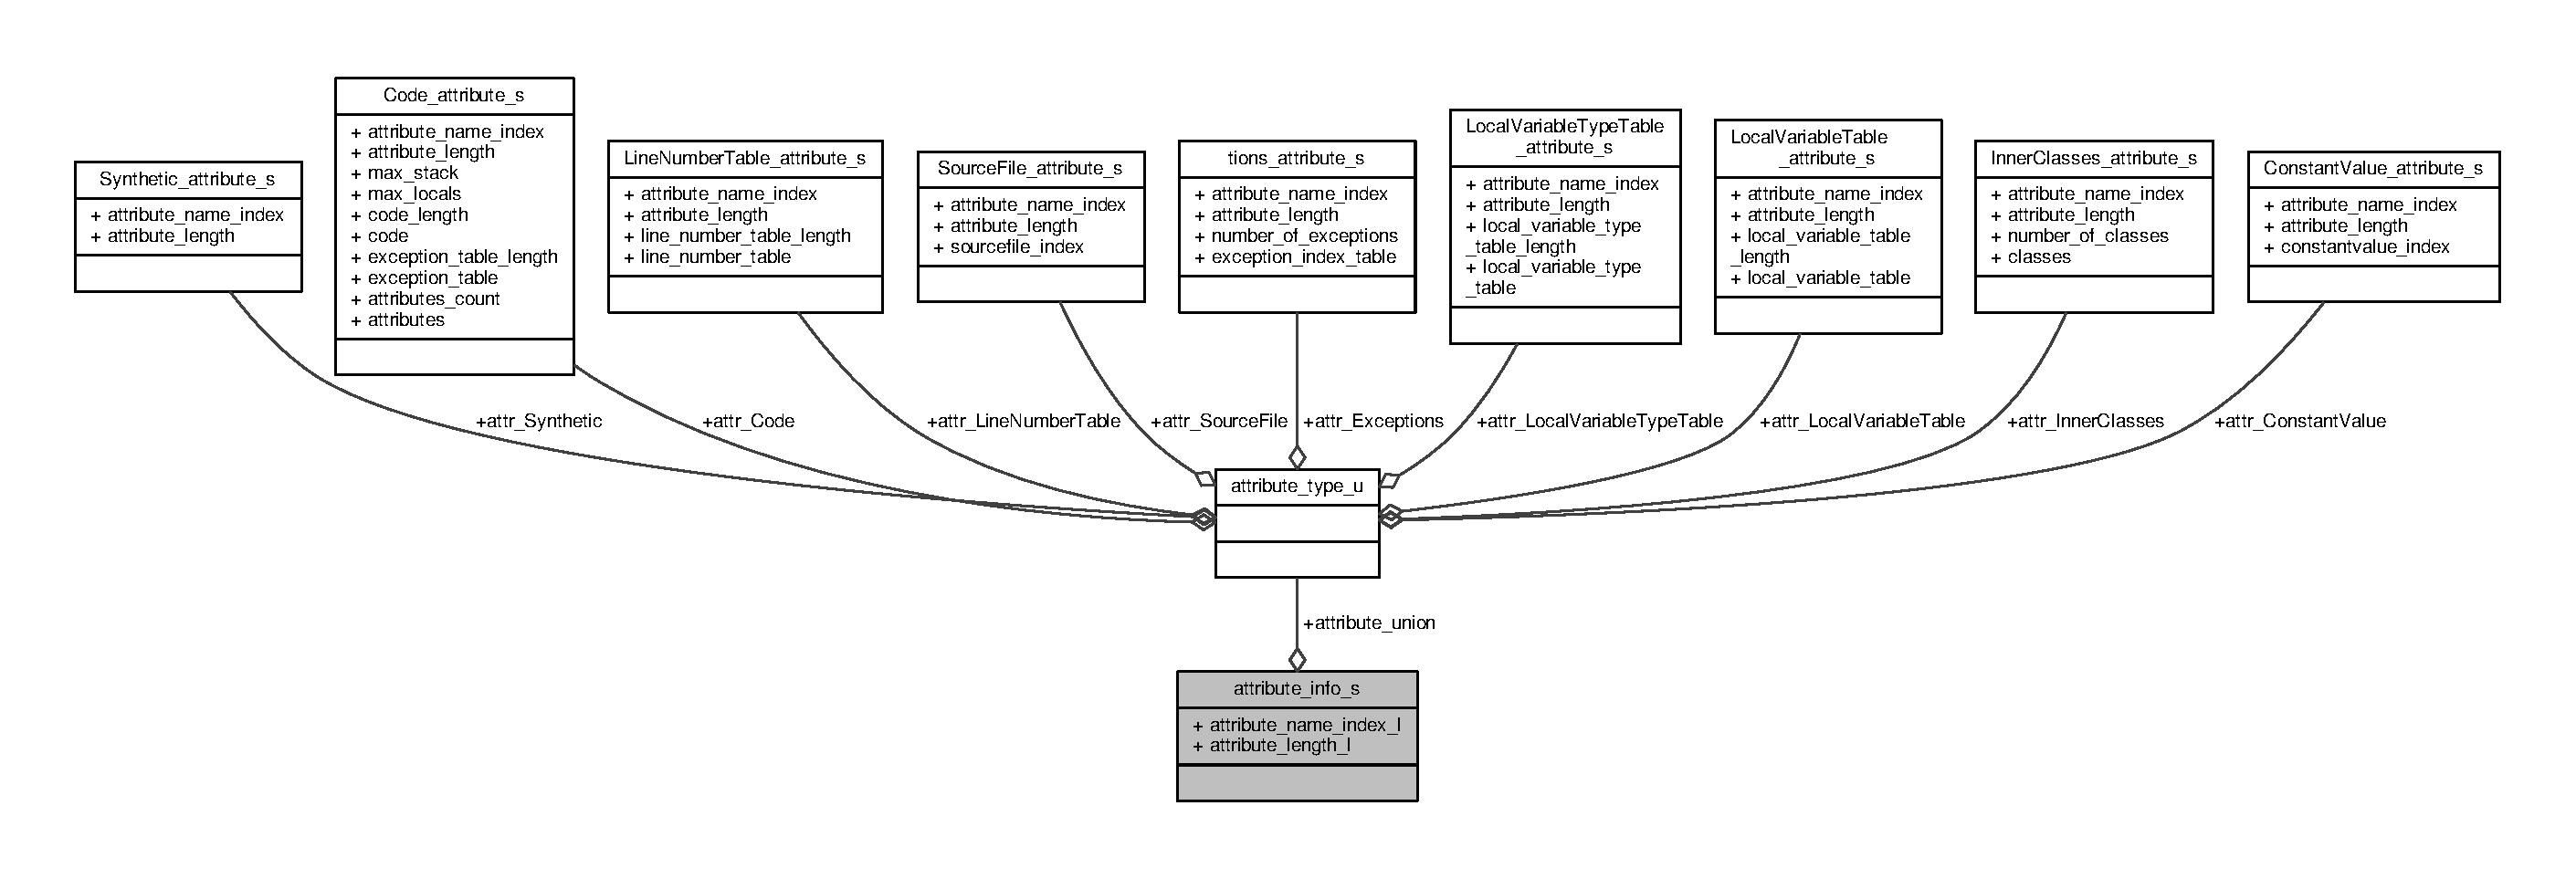
\includegraphics[width=350pt]{structattribute__info__s__coll__graph}
\end{center}
\end{figure}
\subsection*{Public Attributes}
\begin{DoxyCompactItemize}
\item 
uint16\+\_\+t \hyperlink{structattribute__info__s_a21689252627ef43920efed54f5a9e69e}{attribute\+\_\+name\+\_\+index\+\_\+l}
\item 
uint32\+\_\+t \hyperlink{structattribute__info__s_a05108c8ce025ccef6f5dd8f2db872253}{attribute\+\_\+length\+\_\+l}
\item 
\hyperlink{attributes_8hpp_a1f6857b772af6ea7fc2f978b57567f0d}{attribute\+Type\+\_\+u} \hyperlink{structattribute__info__s_a1ca989905be28a2dfe09758a89593b91}{attribute\+\_\+union}
\end{DoxyCompactItemize}


\subsection{Member Data Documentation}
\hypertarget{structattribute__info__s_a05108c8ce025ccef6f5dd8f2db872253}{\index{attribute\+\_\+info\+\_\+s@{attribute\+\_\+info\+\_\+s}!attribute\+\_\+length\+\_\+l@{attribute\+\_\+length\+\_\+l}}
\index{attribute\+\_\+length\+\_\+l@{attribute\+\_\+length\+\_\+l}!attribute\+\_\+info\+\_\+s@{attribute\+\_\+info\+\_\+s}}
\subsubsection[{attribute\+\_\+length\+\_\+l}]{\setlength{\rightskip}{0pt plus 5cm}uint32\+\_\+t attribute\+\_\+info\+\_\+s\+::attribute\+\_\+length\+\_\+l}}\label{structattribute__info__s_a05108c8ce025ccef6f5dd8f2db872253}
\hypertarget{structattribute__info__s_a21689252627ef43920efed54f5a9e69e}{\index{attribute\+\_\+info\+\_\+s@{attribute\+\_\+info\+\_\+s}!attribute\+\_\+name\+\_\+index\+\_\+l@{attribute\+\_\+name\+\_\+index\+\_\+l}}
\index{attribute\+\_\+name\+\_\+index\+\_\+l@{attribute\+\_\+name\+\_\+index\+\_\+l}!attribute\+\_\+info\+\_\+s@{attribute\+\_\+info\+\_\+s}}
\subsubsection[{attribute\+\_\+name\+\_\+index\+\_\+l}]{\setlength{\rightskip}{0pt plus 5cm}uint16\+\_\+t attribute\+\_\+info\+\_\+s\+::attribute\+\_\+name\+\_\+index\+\_\+l}}\label{structattribute__info__s_a21689252627ef43920efed54f5a9e69e}
\hypertarget{structattribute__info__s_a1ca989905be28a2dfe09758a89593b91}{\index{attribute\+\_\+info\+\_\+s@{attribute\+\_\+info\+\_\+s}!attribute\+\_\+union@{attribute\+\_\+union}}
\index{attribute\+\_\+union@{attribute\+\_\+union}!attribute\+\_\+info\+\_\+s@{attribute\+\_\+info\+\_\+s}}
\subsubsection[{attribute\+\_\+union}]{\setlength{\rightskip}{0pt plus 5cm}{\bf attribute\+Type\+\_\+u} attribute\+\_\+info\+\_\+s\+::attribute\+\_\+union}}\label{structattribute__info__s_a1ca989905be28a2dfe09758a89593b91}


The documentation for this struct was generated from the following file\+:\begin{DoxyCompactItemize}
\item 
include/\hyperlink{attributes_8hpp}{attributes.\+hpp}\end{DoxyCompactItemize}

\hypertarget{unionattribute__type__u}{\section{attribute\+\_\+type\+\_\+u Union Reference}
\label{unionattribute__type__u}\index{attribute\+\_\+type\+\_\+u@{attribute\+\_\+type\+\_\+u}}
}


{\ttfamily \#include $<$attributes.\+hpp$>$}



Collaboration diagram for attribute\+\_\+type\+\_\+u\+:\nopagebreak
\begin{figure}[H]
\begin{center}
\leavevmode
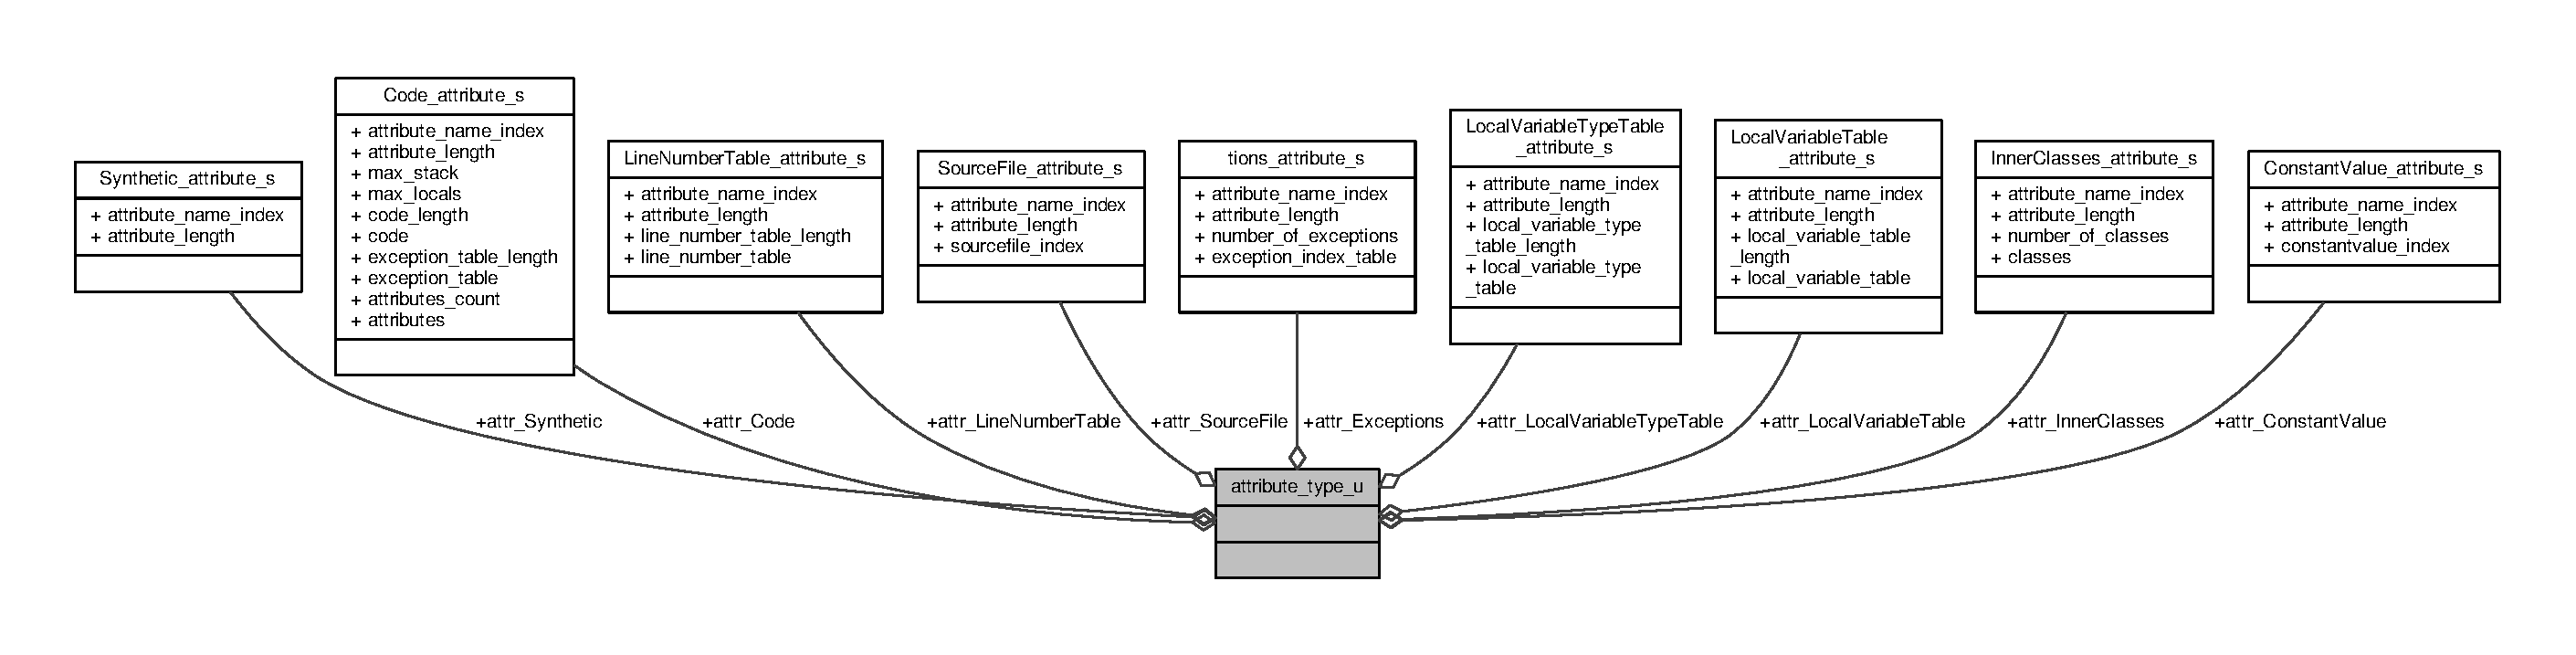
\includegraphics[width=350pt]{unionattribute__type__u__coll__graph}
\end{center}
\end{figure}
\subsection*{Public Attributes}
\begin{DoxyCompactItemize}
\item 
\hyperlink{attributes_8hpp_a11c3b261bde2a1da5fc73081cf62b4db}{Inner\+Classes\+\_\+attribute} \hyperlink{unionattribute__type__u_ade2324dcae8d2af69ed74c6ee6480a69}{attr\+\_\+\+Inner\+Classes}
\item 
\hyperlink{attributes_8hpp_af2b24f13bd3e5a26936bd16e72a76fff}{Line\+Number\+Table\+\_\+attribute} \hyperlink{unionattribute__type__u_ab8c71326a60a1e11695399dd2d123407}{attr\+\_\+\+Line\+Number\+Table}
\item 
\hyperlink{attributes_8hpp_a2985a5f278e47c68777158d1feac4d4f}{Local\+Variable\+Table\+\_\+attribute} \hyperlink{unionattribute__type__u_ad493b7616916c1499908c8a5faee1eb6}{attr\+\_\+\+Local\+Variable\+Table}
\item 
\hyperlink{attributes_8hpp_a5a25e5296f4e3d6a99598ff645e598f2}{Local\+Variable\+Type\+Table\+\_\+attribute} \hyperlink{unionattribute__type__u_ab4b51f1bb761ece948234b28200a9b7f}{attr\+\_\+\+Local\+Variable\+Type\+Table}
\item 
\hyperlink{attributes_8hpp_a4df3241aeeb4382aa355a8c4e4e6076e}{Constant\+Value\+\_\+attribute} \hyperlink{unionattribute__type__u_aaf4ebb5b100f6eab33f2da8a73f7415d}{attr\+\_\+\+Constant\+Value}
\item 
\hyperlink{attributes_8hpp_a493a40fa668908ed61dbb1f823d213ca}{Source\+File\+\_\+attribute} \hyperlink{unionattribute__type__u_aa43db97645b252b9af59f64077bafcca}{attr\+\_\+\+Source\+File}
\item 
\hyperlink{attributes_8hpp_a7dfc4097d3a6cf1ac27bf4ac345e7c99}{Synthetic\+\_\+attribute} \hyperlink{unionattribute__type__u_a148433b2820836cd82e91bf47761812a}{attr\+\_\+\+Synthetic}
\item 
\hyperlink{attributes_8hpp_ad1d2692bc09d9023430faad186e7647e}{Code\+\_\+attribute} \hyperlink{unionattribute__type__u_ad81e10d3ce60b779a53e25f9cbaeb550}{attr\+\_\+\+Code}
\item 
\hyperlink{attributes_8hpp_a472ae3f91d9dfb17a0125bd633c0a3ce}{Exceptions\+\_\+attribute} \hyperlink{unionattribute__type__u_a55eaf900114a14bb34695e1c0e3fe97c}{attr\+\_\+\+Exceptions}
\end{DoxyCompactItemize}


\subsection{Member Data Documentation}
\hypertarget{unionattribute__type__u_ad81e10d3ce60b779a53e25f9cbaeb550}{\index{attribute\+\_\+type\+\_\+u@{attribute\+\_\+type\+\_\+u}!attr\+\_\+\+Code@{attr\+\_\+\+Code}}
\index{attr\+\_\+\+Code@{attr\+\_\+\+Code}!attribute\+\_\+type\+\_\+u@{attribute\+\_\+type\+\_\+u}}
\subsubsection[{attr\+\_\+\+Code}]{\setlength{\rightskip}{0pt plus 5cm}{\bf Code\+\_\+attribute} attribute\+\_\+type\+\_\+u\+::attr\+\_\+\+Code}}\label{unionattribute__type__u_ad81e10d3ce60b779a53e25f9cbaeb550}
\hypertarget{unionattribute__type__u_aaf4ebb5b100f6eab33f2da8a73f7415d}{\index{attribute\+\_\+type\+\_\+u@{attribute\+\_\+type\+\_\+u}!attr\+\_\+\+Constant\+Value@{attr\+\_\+\+Constant\+Value}}
\index{attr\+\_\+\+Constant\+Value@{attr\+\_\+\+Constant\+Value}!attribute\+\_\+type\+\_\+u@{attribute\+\_\+type\+\_\+u}}
\subsubsection[{attr\+\_\+\+Constant\+Value}]{\setlength{\rightskip}{0pt plus 5cm}{\bf Constant\+Value\+\_\+attribute} attribute\+\_\+type\+\_\+u\+::attr\+\_\+\+Constant\+Value}}\label{unionattribute__type__u_aaf4ebb5b100f6eab33f2da8a73f7415d}
\hypertarget{unionattribute__type__u_a55eaf900114a14bb34695e1c0e3fe97c}{\index{attribute\+\_\+type\+\_\+u@{attribute\+\_\+type\+\_\+u}!attr\+\_\+\+Exceptions@{attr\+\_\+\+Exceptions}}
\index{attr\+\_\+\+Exceptions@{attr\+\_\+\+Exceptions}!attribute\+\_\+type\+\_\+u@{attribute\+\_\+type\+\_\+u}}
\subsubsection[{attr\+\_\+\+Exceptions}]{\setlength{\rightskip}{0pt plus 5cm}{\bf Exceptions\+\_\+attribute} attribute\+\_\+type\+\_\+u\+::attr\+\_\+\+Exceptions}}\label{unionattribute__type__u_a55eaf900114a14bb34695e1c0e3fe97c}
\hypertarget{unionattribute__type__u_ade2324dcae8d2af69ed74c6ee6480a69}{\index{attribute\+\_\+type\+\_\+u@{attribute\+\_\+type\+\_\+u}!attr\+\_\+\+Inner\+Classes@{attr\+\_\+\+Inner\+Classes}}
\index{attr\+\_\+\+Inner\+Classes@{attr\+\_\+\+Inner\+Classes}!attribute\+\_\+type\+\_\+u@{attribute\+\_\+type\+\_\+u}}
\subsubsection[{attr\+\_\+\+Inner\+Classes}]{\setlength{\rightskip}{0pt plus 5cm}{\bf Inner\+Classes\+\_\+attribute} attribute\+\_\+type\+\_\+u\+::attr\+\_\+\+Inner\+Classes}}\label{unionattribute__type__u_ade2324dcae8d2af69ed74c6ee6480a69}
\hypertarget{unionattribute__type__u_ab8c71326a60a1e11695399dd2d123407}{\index{attribute\+\_\+type\+\_\+u@{attribute\+\_\+type\+\_\+u}!attr\+\_\+\+Line\+Number\+Table@{attr\+\_\+\+Line\+Number\+Table}}
\index{attr\+\_\+\+Line\+Number\+Table@{attr\+\_\+\+Line\+Number\+Table}!attribute\+\_\+type\+\_\+u@{attribute\+\_\+type\+\_\+u}}
\subsubsection[{attr\+\_\+\+Line\+Number\+Table}]{\setlength{\rightskip}{0pt plus 5cm}{\bf Line\+Number\+Table\+\_\+attribute} attribute\+\_\+type\+\_\+u\+::attr\+\_\+\+Line\+Number\+Table}}\label{unionattribute__type__u_ab8c71326a60a1e11695399dd2d123407}
\hypertarget{unionattribute__type__u_ad493b7616916c1499908c8a5faee1eb6}{\index{attribute\+\_\+type\+\_\+u@{attribute\+\_\+type\+\_\+u}!attr\+\_\+\+Local\+Variable\+Table@{attr\+\_\+\+Local\+Variable\+Table}}
\index{attr\+\_\+\+Local\+Variable\+Table@{attr\+\_\+\+Local\+Variable\+Table}!attribute\+\_\+type\+\_\+u@{attribute\+\_\+type\+\_\+u}}
\subsubsection[{attr\+\_\+\+Local\+Variable\+Table}]{\setlength{\rightskip}{0pt plus 5cm}{\bf Local\+Variable\+Table\+\_\+attribute} attribute\+\_\+type\+\_\+u\+::attr\+\_\+\+Local\+Variable\+Table}}\label{unionattribute__type__u_ad493b7616916c1499908c8a5faee1eb6}
\hypertarget{unionattribute__type__u_ab4b51f1bb761ece948234b28200a9b7f}{\index{attribute\+\_\+type\+\_\+u@{attribute\+\_\+type\+\_\+u}!attr\+\_\+\+Local\+Variable\+Type\+Table@{attr\+\_\+\+Local\+Variable\+Type\+Table}}
\index{attr\+\_\+\+Local\+Variable\+Type\+Table@{attr\+\_\+\+Local\+Variable\+Type\+Table}!attribute\+\_\+type\+\_\+u@{attribute\+\_\+type\+\_\+u}}
\subsubsection[{attr\+\_\+\+Local\+Variable\+Type\+Table}]{\setlength{\rightskip}{0pt plus 5cm}{\bf Local\+Variable\+Type\+Table\+\_\+attribute} attribute\+\_\+type\+\_\+u\+::attr\+\_\+\+Local\+Variable\+Type\+Table}}\label{unionattribute__type__u_ab4b51f1bb761ece948234b28200a9b7f}
\hypertarget{unionattribute__type__u_aa43db97645b252b9af59f64077bafcca}{\index{attribute\+\_\+type\+\_\+u@{attribute\+\_\+type\+\_\+u}!attr\+\_\+\+Source\+File@{attr\+\_\+\+Source\+File}}
\index{attr\+\_\+\+Source\+File@{attr\+\_\+\+Source\+File}!attribute\+\_\+type\+\_\+u@{attribute\+\_\+type\+\_\+u}}
\subsubsection[{attr\+\_\+\+Source\+File}]{\setlength{\rightskip}{0pt plus 5cm}{\bf Source\+File\+\_\+attribute} attribute\+\_\+type\+\_\+u\+::attr\+\_\+\+Source\+File}}\label{unionattribute__type__u_aa43db97645b252b9af59f64077bafcca}
\hypertarget{unionattribute__type__u_a148433b2820836cd82e91bf47761812a}{\index{attribute\+\_\+type\+\_\+u@{attribute\+\_\+type\+\_\+u}!attr\+\_\+\+Synthetic@{attr\+\_\+\+Synthetic}}
\index{attr\+\_\+\+Synthetic@{attr\+\_\+\+Synthetic}!attribute\+\_\+type\+\_\+u@{attribute\+\_\+type\+\_\+u}}
\subsubsection[{attr\+\_\+\+Synthetic}]{\setlength{\rightskip}{0pt plus 5cm}{\bf Synthetic\+\_\+attribute} attribute\+\_\+type\+\_\+u\+::attr\+\_\+\+Synthetic}}\label{unionattribute__type__u_a148433b2820836cd82e91bf47761812a}


The documentation for this union was generated from the following file\+:\begin{DoxyCompactItemize}
\item 
include/\hyperlink{attributes_8hpp}{attributes.\+hpp}\end{DoxyCompactItemize}

\hypertarget{structclasses__info__s}{\section{classes\+\_\+info\+\_\+s Struct Reference}
\label{structclasses__info__s}\index{classes\+\_\+info\+\_\+s@{classes\+\_\+info\+\_\+s}}
}


{\ttfamily \#include $<$attributes.\+hpp$>$}



Collaboration diagram for classes\+\_\+info\+\_\+s\+:\nopagebreak
\begin{figure}[H]
\begin{center}
\leavevmode
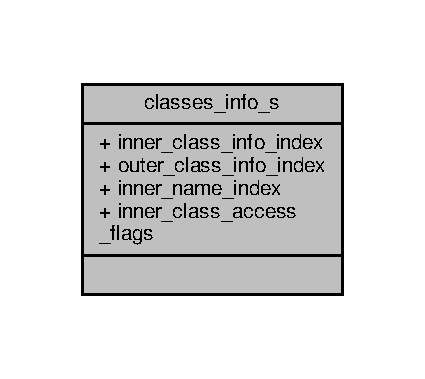
\includegraphics[width=204pt]{structclasses__info__s__coll__graph}
\end{center}
\end{figure}
\subsection*{Public Attributes}
\begin{DoxyCompactItemize}
\item 
uint16\+\_\+t \hyperlink{structclasses__info__s_ae8c45ace1c34dd137289f54f5d5704c3}{inner\+\_\+class\+\_\+info\+\_\+index}
\item 
uint16\+\_\+t \hyperlink{structclasses__info__s_a25b561f15295b3ea0d55932ee4f00260}{outer\+\_\+class\+\_\+info\+\_\+index}
\item 
uint16\+\_\+t \hyperlink{structclasses__info__s_ac33145154cb1f0db33d90e02800b00bb}{inner\+\_\+name\+\_\+index}
\item 
uint16\+\_\+t \hyperlink{structclasses__info__s_a821ed8a4eabdf77102409c67bb0d519f}{inner\+\_\+class\+\_\+access\+\_\+flags}
\end{DoxyCompactItemize}


\subsection{Member Data Documentation}
\hypertarget{structclasses__info__s_a821ed8a4eabdf77102409c67bb0d519f}{\index{classes\+\_\+info\+\_\+s@{classes\+\_\+info\+\_\+s}!inner\+\_\+class\+\_\+access\+\_\+flags@{inner\+\_\+class\+\_\+access\+\_\+flags}}
\index{inner\+\_\+class\+\_\+access\+\_\+flags@{inner\+\_\+class\+\_\+access\+\_\+flags}!classes\+\_\+info\+\_\+s@{classes\+\_\+info\+\_\+s}}
\subsubsection[{inner\+\_\+class\+\_\+access\+\_\+flags}]{\setlength{\rightskip}{0pt plus 5cm}uint16\+\_\+t classes\+\_\+info\+\_\+s\+::inner\+\_\+class\+\_\+access\+\_\+flags}}\label{structclasses__info__s_a821ed8a4eabdf77102409c67bb0d519f}
\hypertarget{structclasses__info__s_ae8c45ace1c34dd137289f54f5d5704c3}{\index{classes\+\_\+info\+\_\+s@{classes\+\_\+info\+\_\+s}!inner\+\_\+class\+\_\+info\+\_\+index@{inner\+\_\+class\+\_\+info\+\_\+index}}
\index{inner\+\_\+class\+\_\+info\+\_\+index@{inner\+\_\+class\+\_\+info\+\_\+index}!classes\+\_\+info\+\_\+s@{classes\+\_\+info\+\_\+s}}
\subsubsection[{inner\+\_\+class\+\_\+info\+\_\+index}]{\setlength{\rightskip}{0pt plus 5cm}uint16\+\_\+t classes\+\_\+info\+\_\+s\+::inner\+\_\+class\+\_\+info\+\_\+index}}\label{structclasses__info__s_ae8c45ace1c34dd137289f54f5d5704c3}
\hypertarget{structclasses__info__s_ac33145154cb1f0db33d90e02800b00bb}{\index{classes\+\_\+info\+\_\+s@{classes\+\_\+info\+\_\+s}!inner\+\_\+name\+\_\+index@{inner\+\_\+name\+\_\+index}}
\index{inner\+\_\+name\+\_\+index@{inner\+\_\+name\+\_\+index}!classes\+\_\+info\+\_\+s@{classes\+\_\+info\+\_\+s}}
\subsubsection[{inner\+\_\+name\+\_\+index}]{\setlength{\rightskip}{0pt plus 5cm}uint16\+\_\+t classes\+\_\+info\+\_\+s\+::inner\+\_\+name\+\_\+index}}\label{structclasses__info__s_ac33145154cb1f0db33d90e02800b00bb}
\hypertarget{structclasses__info__s_a25b561f15295b3ea0d55932ee4f00260}{\index{classes\+\_\+info\+\_\+s@{classes\+\_\+info\+\_\+s}!outer\+\_\+class\+\_\+info\+\_\+index@{outer\+\_\+class\+\_\+info\+\_\+index}}
\index{outer\+\_\+class\+\_\+info\+\_\+index@{outer\+\_\+class\+\_\+info\+\_\+index}!classes\+\_\+info\+\_\+s@{classes\+\_\+info\+\_\+s}}
\subsubsection[{outer\+\_\+class\+\_\+info\+\_\+index}]{\setlength{\rightskip}{0pt plus 5cm}uint16\+\_\+t classes\+\_\+info\+\_\+s\+::outer\+\_\+class\+\_\+info\+\_\+index}}\label{structclasses__info__s_a25b561f15295b3ea0d55932ee4f00260}


The documentation for this struct was generated from the following file\+:\begin{DoxyCompactItemize}
\item 
include/\hyperlink{attributes_8hpp}{attributes.\+hpp}\end{DoxyCompactItemize}

\hypertarget{classClassFile}{\section{Class\+File Class Reference}
\label{classClassFile}\index{Class\+File@{Class\+File}}
}


{\ttfamily \#include $<$class\+File.\+hpp$>$}



Collaboration diagram for Class\+File\+:\nopagebreak
\begin{figure}[H]
\begin{center}
\leavevmode
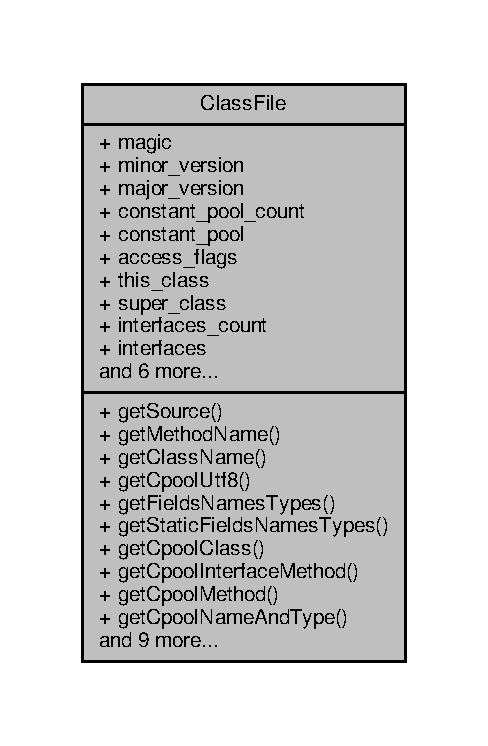
\includegraphics[width=210pt]{classClassFile__coll__graph}
\end{center}
\end{figure}
\subsection*{Public Member Functions}
\begin{DoxyCompactItemize}
\item 
std\+::string \hyperlink{classClassFile_a327e97890dd251532d064da9aa61deeb}{get\+Source} ()
\item 
std\+::string \hyperlink{classClassFile_a325315e2b9ccf9c10955467aae82b2a1}{get\+Class\+Name} ()
\item 
std\+::string \hyperlink{classClassFile_a917fdac173079a7eebacb22b728f295d}{get\+Cpool\+Utf8} (int index)
\item 
std\+::map$<$ std\+::string, \\*
std\+::string $>$ \hyperlink{classClassFile_aa791a7b86ab130ba6ba28d6d71f2c70c}{get\+Fields\+Names\+Types} ()
\item 
int \hyperlink{classClassFile_ab67b335ccd0e88ddb3b8ab99a602b8ea}{find\+Main} ()
\item 
char $\ast$ \hyperlink{classClassFile_a4d350fc2fcad87ab085c795adef1fe12}{get\+Name} (int name\+\_\+index)
\item 
\hyperlink{attributes_8hpp_ad1d2692bc09d9023430faad186e7647e}{Code\+\_\+attribute} $\ast$ \hyperlink{classClassFile_a3c6a5ced9d8616700fa2eef615489724}{get\+Code\+Attr} (\hyperlink{structs_8hpp_a6cbc7230791f4ca5e82816e58baeeacc}{method\+\_\+info} $\ast$method)
\end{DoxyCompactItemize}
\subsection*{Public Attributes}
\begin{DoxyCompactItemize}
\item 
uint32\+\_\+t \hyperlink{classClassFile_a9d4d72751ff9250dd3305d5d853f7921}{magic}
\item 
uint16\+\_\+t \hyperlink{classClassFile_a357116b538d1b1ef11073560eba9396d}{minor\+\_\+version}
\item 
uint16\+\_\+t \hyperlink{classClassFile_a931ebda6a22c18e009891d40016b2790}{major\+\_\+version}
\item 
uint32\+\_\+t \hyperlink{classClassFile_a76abb829a9ebb954e9ef381f144bdbf9}{constant\+\_\+pool\+\_\+count}
\item 
std\+::vector$<$ \hyperlink{structs_8hpp_a0c0d87e91cda2669bf03488501eccd4d}{cp\+\_\+info} $>$ \hyperlink{classClassFile_aecb7bcd6074a0dbda85dea876a691187}{constant\+\_\+pool}
\item 
uint16\+\_\+t \hyperlink{classClassFile_a2d095ef980330834af44c587ce52590e}{access\+\_\+flags}
\item 
uint16\+\_\+t \hyperlink{classClassFile_aa45abc9545fe11fca252d9769b665294}{this\+\_\+class}
\item 
uint16\+\_\+t \hyperlink{classClassFile_aa48f683b6e5b60021410f88a5e831cbe}{super\+\_\+class}
\item 
uint16\+\_\+t \hyperlink{classClassFile_a25f384f7a9746352aad90fb499126704}{interfaces\+\_\+count}
\item 
std\+::vector$<$ uint16\+\_\+t $>$ \hyperlink{classClassFile_a5ff706f77d13aa4cd2876e6a083ed849}{interfaces}
\item 
uint16\+\_\+t \hyperlink{classClassFile_a517d14b0d9e507f1485a3b6d3cb38683}{fields\+\_\+count}
\item 
std\+::vector$<$ \hyperlink{structs_8hpp_a9dec70227361c4b10468fe98e7b8d2ab}{field\+\_\+info} $>$ \hyperlink{classClassFile_adf8e8ff620c2e938c5bcb8616e754ce3}{fields}
\item 
uint16\+\_\+t \hyperlink{classClassFile_a479310e3e0674d9171d24beb794fcb14}{methods\+\_\+count}
\item 
std\+::vector$<$ \hyperlink{structs_8hpp_a6cbc7230791f4ca5e82816e58baeeacc}{method\+\_\+info} $>$ \hyperlink{classClassFile_ab1f087a706ccd7f5334bd17ed4d05936}{methods}
\item 
uint16\+\_\+t \hyperlink{classClassFile_accd99ee441c45eb8fdcd3836d56e9ef4}{attributes\+\_\+count}
\item 
std\+::vector$<$ \hyperlink{attributes_8hpp_a7af51299ff517acce960ac87c9db9899}{attribute\+\_\+info} $>$ \hyperlink{classClassFile_a119011b9d84894da116c83fa6539d5ce}{attributes}
\end{DoxyCompactItemize}


\subsection{Member Function Documentation}
\hypertarget{classClassFile_ab67b335ccd0e88ddb3b8ab99a602b8ea}{\index{Class\+File@{Class\+File}!find\+Main@{find\+Main}}
\index{find\+Main@{find\+Main}!Class\+File@{Class\+File}}
\subsubsection[{find\+Main}]{\setlength{\rightskip}{0pt plus 5cm}int Class\+File\+::find\+Main (
\begin{DoxyParamCaption}
{}
\end{DoxyParamCaption}
)}}\label{classClassFile_ab67b335ccd0e88ddb3b8ab99a602b8ea}
\hypertarget{classClassFile_a325315e2b9ccf9c10955467aae82b2a1}{\index{Class\+File@{Class\+File}!get\+Class\+Name@{get\+Class\+Name}}
\index{get\+Class\+Name@{get\+Class\+Name}!Class\+File@{Class\+File}}
\subsubsection[{get\+Class\+Name}]{\setlength{\rightskip}{0pt plus 5cm}string Class\+File\+::get\+Class\+Name (
\begin{DoxyParamCaption}
{}
\end{DoxyParamCaption}
)}}\label{classClassFile_a325315e2b9ccf9c10955467aae82b2a1}
\hypertarget{classClassFile_a3c6a5ced9d8616700fa2eef615489724}{\index{Class\+File@{Class\+File}!get\+Code\+Attr@{get\+Code\+Attr}}
\index{get\+Code\+Attr@{get\+Code\+Attr}!Class\+File@{Class\+File}}
\subsubsection[{get\+Code\+Attr}]{\setlength{\rightskip}{0pt plus 5cm}{\bf Code\+\_\+attribute} $\ast$ Class\+File\+::get\+Code\+Attr (
\begin{DoxyParamCaption}
\item[{{\bf method\+\_\+info} $\ast$}]{method}
\end{DoxyParamCaption}
)}}\label{classClassFile_a3c6a5ced9d8616700fa2eef615489724}
\hypertarget{classClassFile_a917fdac173079a7eebacb22b728f295d}{\index{Class\+File@{Class\+File}!get\+Cpool\+Utf8@{get\+Cpool\+Utf8}}
\index{get\+Cpool\+Utf8@{get\+Cpool\+Utf8}!Class\+File@{Class\+File}}
\subsubsection[{get\+Cpool\+Utf8}]{\setlength{\rightskip}{0pt plus 5cm}string Class\+File\+::get\+Cpool\+Utf8 (
\begin{DoxyParamCaption}
\item[{int}]{index}
\end{DoxyParamCaption}
)}}\label{classClassFile_a917fdac173079a7eebacb22b728f295d}
\hypertarget{classClassFile_aa791a7b86ab130ba6ba28d6d71f2c70c}{\index{Class\+File@{Class\+File}!get\+Fields\+Names\+Types@{get\+Fields\+Names\+Types}}
\index{get\+Fields\+Names\+Types@{get\+Fields\+Names\+Types}!Class\+File@{Class\+File}}
\subsubsection[{get\+Fields\+Names\+Types}]{\setlength{\rightskip}{0pt plus 5cm}map$<$ string, string $>$ Class\+File\+::get\+Fields\+Names\+Types (
\begin{DoxyParamCaption}
{}
\end{DoxyParamCaption}
)}}\label{classClassFile_aa791a7b86ab130ba6ba28d6d71f2c70c}
\hypertarget{classClassFile_a4d350fc2fcad87ab085c795adef1fe12}{\index{Class\+File@{Class\+File}!get\+Name@{get\+Name}}
\index{get\+Name@{get\+Name}!Class\+File@{Class\+File}}
\subsubsection[{get\+Name}]{\setlength{\rightskip}{0pt plus 5cm}char $\ast$ Class\+File\+::get\+Name (
\begin{DoxyParamCaption}
\item[{int}]{name\+\_\+index}
\end{DoxyParamCaption}
)}}\label{classClassFile_a4d350fc2fcad87ab085c795adef1fe12}
\hypertarget{classClassFile_a327e97890dd251532d064da9aa61deeb}{\index{Class\+File@{Class\+File}!get\+Source@{get\+Source}}
\index{get\+Source@{get\+Source}!Class\+File@{Class\+File}}
\subsubsection[{get\+Source}]{\setlength{\rightskip}{0pt plus 5cm}string Class\+File\+::get\+Source (
\begin{DoxyParamCaption}
{}
\end{DoxyParamCaption}
)}}\label{classClassFile_a327e97890dd251532d064da9aa61deeb}


\subsection{Member Data Documentation}
\hypertarget{classClassFile_a2d095ef980330834af44c587ce52590e}{\index{Class\+File@{Class\+File}!access\+\_\+flags@{access\+\_\+flags}}
\index{access\+\_\+flags@{access\+\_\+flags}!Class\+File@{Class\+File}}
\subsubsection[{access\+\_\+flags}]{\setlength{\rightskip}{0pt plus 5cm}uint16\+\_\+t Class\+File\+::access\+\_\+flags}}\label{classClassFile_a2d095ef980330834af44c587ce52590e}
\hypertarget{classClassFile_a119011b9d84894da116c83fa6539d5ce}{\index{Class\+File@{Class\+File}!attributes@{attributes}}
\index{attributes@{attributes}!Class\+File@{Class\+File}}
\subsubsection[{attributes}]{\setlength{\rightskip}{0pt plus 5cm}std\+::vector$<${\bf attribute\+\_\+info}$>$ Class\+File\+::attributes}}\label{classClassFile_a119011b9d84894da116c83fa6539d5ce}
\hypertarget{classClassFile_accd99ee441c45eb8fdcd3836d56e9ef4}{\index{Class\+File@{Class\+File}!attributes\+\_\+count@{attributes\+\_\+count}}
\index{attributes\+\_\+count@{attributes\+\_\+count}!Class\+File@{Class\+File}}
\subsubsection[{attributes\+\_\+count}]{\setlength{\rightskip}{0pt plus 5cm}uint16\+\_\+t Class\+File\+::attributes\+\_\+count}}\label{classClassFile_accd99ee441c45eb8fdcd3836d56e9ef4}
\hypertarget{classClassFile_aecb7bcd6074a0dbda85dea876a691187}{\index{Class\+File@{Class\+File}!constant\+\_\+pool@{constant\+\_\+pool}}
\index{constant\+\_\+pool@{constant\+\_\+pool}!Class\+File@{Class\+File}}
\subsubsection[{constant\+\_\+pool}]{\setlength{\rightskip}{0pt plus 5cm}std\+::vector$<${\bf cp\+\_\+info}$>$ Class\+File\+::constant\+\_\+pool}}\label{classClassFile_aecb7bcd6074a0dbda85dea876a691187}
\hypertarget{classClassFile_a76abb829a9ebb954e9ef381f144bdbf9}{\index{Class\+File@{Class\+File}!constant\+\_\+pool\+\_\+count@{constant\+\_\+pool\+\_\+count}}
\index{constant\+\_\+pool\+\_\+count@{constant\+\_\+pool\+\_\+count}!Class\+File@{Class\+File}}
\subsubsection[{constant\+\_\+pool\+\_\+count}]{\setlength{\rightskip}{0pt plus 5cm}uint32\+\_\+t Class\+File\+::constant\+\_\+pool\+\_\+count}}\label{classClassFile_a76abb829a9ebb954e9ef381f144bdbf9}
\hypertarget{classClassFile_adf8e8ff620c2e938c5bcb8616e754ce3}{\index{Class\+File@{Class\+File}!fields@{fields}}
\index{fields@{fields}!Class\+File@{Class\+File}}
\subsubsection[{fields}]{\setlength{\rightskip}{0pt plus 5cm}std\+::vector$<${\bf field\+\_\+info}$>$ Class\+File\+::fields}}\label{classClassFile_adf8e8ff620c2e938c5bcb8616e754ce3}
\hypertarget{classClassFile_a517d14b0d9e507f1485a3b6d3cb38683}{\index{Class\+File@{Class\+File}!fields\+\_\+count@{fields\+\_\+count}}
\index{fields\+\_\+count@{fields\+\_\+count}!Class\+File@{Class\+File}}
\subsubsection[{fields\+\_\+count}]{\setlength{\rightskip}{0pt plus 5cm}uint16\+\_\+t Class\+File\+::fields\+\_\+count}}\label{classClassFile_a517d14b0d9e507f1485a3b6d3cb38683}
\hypertarget{classClassFile_a5ff706f77d13aa4cd2876e6a083ed849}{\index{Class\+File@{Class\+File}!interfaces@{interfaces}}
\index{interfaces@{interfaces}!Class\+File@{Class\+File}}
\subsubsection[{interfaces}]{\setlength{\rightskip}{0pt plus 5cm}std\+::vector$<$uint16\+\_\+t$>$ Class\+File\+::interfaces}}\label{classClassFile_a5ff706f77d13aa4cd2876e6a083ed849}
\hypertarget{classClassFile_a25f384f7a9746352aad90fb499126704}{\index{Class\+File@{Class\+File}!interfaces\+\_\+count@{interfaces\+\_\+count}}
\index{interfaces\+\_\+count@{interfaces\+\_\+count}!Class\+File@{Class\+File}}
\subsubsection[{interfaces\+\_\+count}]{\setlength{\rightskip}{0pt plus 5cm}uint16\+\_\+t Class\+File\+::interfaces\+\_\+count}}\label{classClassFile_a25f384f7a9746352aad90fb499126704}
\hypertarget{classClassFile_a9d4d72751ff9250dd3305d5d853f7921}{\index{Class\+File@{Class\+File}!magic@{magic}}
\index{magic@{magic}!Class\+File@{Class\+File}}
\subsubsection[{magic}]{\setlength{\rightskip}{0pt plus 5cm}uint32\+\_\+t Class\+File\+::magic}}\label{classClassFile_a9d4d72751ff9250dd3305d5d853f7921}
\hypertarget{classClassFile_a931ebda6a22c18e009891d40016b2790}{\index{Class\+File@{Class\+File}!major\+\_\+version@{major\+\_\+version}}
\index{major\+\_\+version@{major\+\_\+version}!Class\+File@{Class\+File}}
\subsubsection[{major\+\_\+version}]{\setlength{\rightskip}{0pt plus 5cm}uint16\+\_\+t Class\+File\+::major\+\_\+version}}\label{classClassFile_a931ebda6a22c18e009891d40016b2790}
\hypertarget{classClassFile_ab1f087a706ccd7f5334bd17ed4d05936}{\index{Class\+File@{Class\+File}!methods@{methods}}
\index{methods@{methods}!Class\+File@{Class\+File}}
\subsubsection[{methods}]{\setlength{\rightskip}{0pt plus 5cm}std\+::vector$<${\bf method\+\_\+info}$>$ Class\+File\+::methods}}\label{classClassFile_ab1f087a706ccd7f5334bd17ed4d05936}
\hypertarget{classClassFile_a479310e3e0674d9171d24beb794fcb14}{\index{Class\+File@{Class\+File}!methods\+\_\+count@{methods\+\_\+count}}
\index{methods\+\_\+count@{methods\+\_\+count}!Class\+File@{Class\+File}}
\subsubsection[{methods\+\_\+count}]{\setlength{\rightskip}{0pt plus 5cm}uint16\+\_\+t Class\+File\+::methods\+\_\+count}}\label{classClassFile_a479310e3e0674d9171d24beb794fcb14}
\hypertarget{classClassFile_a357116b538d1b1ef11073560eba9396d}{\index{Class\+File@{Class\+File}!minor\+\_\+version@{minor\+\_\+version}}
\index{minor\+\_\+version@{minor\+\_\+version}!Class\+File@{Class\+File}}
\subsubsection[{minor\+\_\+version}]{\setlength{\rightskip}{0pt plus 5cm}uint16\+\_\+t Class\+File\+::minor\+\_\+version}}\label{classClassFile_a357116b538d1b1ef11073560eba9396d}
\hypertarget{classClassFile_aa48f683b6e5b60021410f88a5e831cbe}{\index{Class\+File@{Class\+File}!super\+\_\+class@{super\+\_\+class}}
\index{super\+\_\+class@{super\+\_\+class}!Class\+File@{Class\+File}}
\subsubsection[{super\+\_\+class}]{\setlength{\rightskip}{0pt plus 5cm}uint16\+\_\+t Class\+File\+::super\+\_\+class}}\label{classClassFile_aa48f683b6e5b60021410f88a5e831cbe}
\hypertarget{classClassFile_aa45abc9545fe11fca252d9769b665294}{\index{Class\+File@{Class\+File}!this\+\_\+class@{this\+\_\+class}}
\index{this\+\_\+class@{this\+\_\+class}!Class\+File@{Class\+File}}
\subsubsection[{this\+\_\+class}]{\setlength{\rightskip}{0pt plus 5cm}uint16\+\_\+t Class\+File\+::this\+\_\+class}}\label{classClassFile_aa45abc9545fe11fca252d9769b665294}


The documentation for this class was generated from the following files\+:\begin{DoxyCompactItemize}
\item 
include/\hyperlink{classFile_8hpp}{class\+File.\+hpp}\item 
src/\hyperlink{classFile_8cpp}{class\+File.\+cpp}\end{DoxyCompactItemize}

\hypertarget{structCode__attribute__s}{\section{Code\+\_\+attribute\+\_\+s Struct Reference}
\label{structCode__attribute__s}\index{Code\+\_\+attribute\+\_\+s@{Code\+\_\+attribute\+\_\+s}}
}


{\ttfamily \#include $<$attributes.\+hpp$>$}



Collaboration diagram for Code\+\_\+attribute\+\_\+s\+:\nopagebreak
\begin{figure}[H]
\begin{center}
\leavevmode
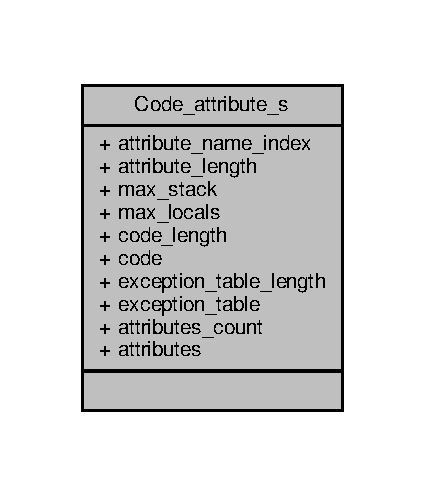
\includegraphics[width=204pt]{structCode__attribute__s__coll__graph}
\end{center}
\end{figure}
\subsection*{Public Attributes}
\begin{DoxyCompactItemize}
\item 
uint16\+\_\+t \hyperlink{structCode__attribute__s_a2ad36c662b25c88553dffda3499b304a}{attribute\+\_\+name\+\_\+index}
\item 
uint32\+\_\+t \hyperlink{structCode__attribute__s_a83fe4677e5b3b8a9fb6460b064148ac3}{attribute\+\_\+length}
\item 
uint16\+\_\+t \hyperlink{structCode__attribute__s_a9f7cd4c713b350f6630949c6364e8e48}{max\+\_\+stack}
\item 
uint16\+\_\+t \hyperlink{structCode__attribute__s_a1c9257d634d9e8473acf1a3d13fac4e7}{max\+\_\+locals}
\item 
uint32\+\_\+t \hyperlink{structCode__attribute__s_ad5cdbcaf02efd1ac9d75d1d1d73d7523}{code\+\_\+length}
\item 
uint8\+\_\+t $\ast$ \hyperlink{structCode__attribute__s_aa8912d50bfd6b1b9bc24cfbb27d33736}{code}
\item 
uint16\+\_\+t \hyperlink{structCode__attribute__s_a73c51a112c0f08db03fe7622279b01e5}{exception\+\_\+table\+\_\+length}
\item 
std\+::vector\\*
$<$ \hyperlink{classexception__table__info}{exception\+\_\+table\+\_\+info} $>$ $\ast$ \hyperlink{structCode__attribute__s_a64c20d58846e4b1af5c4de2a750e8fde}{exception\+\_\+table}
\item 
uint16\+\_\+t \hyperlink{structCode__attribute__s_a12d5860b06a8484744852c38cb79144e}{attributes\+\_\+count}
\item 
std\+::vector$<$ struct \\*
\hyperlink{structattribute__info__s}{attribute\+\_\+info\+\_\+s} $>$ $\ast$ \hyperlink{structCode__attribute__s_a04152c5c6f9f1067d6e144e1e3a814fe}{attributes}
\end{DoxyCompactItemize}


\subsection{Member Data Documentation}
\hypertarget{structCode__attribute__s_a83fe4677e5b3b8a9fb6460b064148ac3}{\index{Code\+\_\+attribute\+\_\+s@{Code\+\_\+attribute\+\_\+s}!attribute\+\_\+length@{attribute\+\_\+length}}
\index{attribute\+\_\+length@{attribute\+\_\+length}!Code\+\_\+attribute\+\_\+s@{Code\+\_\+attribute\+\_\+s}}
\subsubsection[{attribute\+\_\+length}]{\setlength{\rightskip}{0pt plus 5cm}uint32\+\_\+t Code\+\_\+attribute\+\_\+s\+::attribute\+\_\+length}}\label{structCode__attribute__s_a83fe4677e5b3b8a9fb6460b064148ac3}
\hypertarget{structCode__attribute__s_a2ad36c662b25c88553dffda3499b304a}{\index{Code\+\_\+attribute\+\_\+s@{Code\+\_\+attribute\+\_\+s}!attribute\+\_\+name\+\_\+index@{attribute\+\_\+name\+\_\+index}}
\index{attribute\+\_\+name\+\_\+index@{attribute\+\_\+name\+\_\+index}!Code\+\_\+attribute\+\_\+s@{Code\+\_\+attribute\+\_\+s}}
\subsubsection[{attribute\+\_\+name\+\_\+index}]{\setlength{\rightskip}{0pt plus 5cm}uint16\+\_\+t Code\+\_\+attribute\+\_\+s\+::attribute\+\_\+name\+\_\+index}}\label{structCode__attribute__s_a2ad36c662b25c88553dffda3499b304a}
\hypertarget{structCode__attribute__s_a04152c5c6f9f1067d6e144e1e3a814fe}{\index{Code\+\_\+attribute\+\_\+s@{Code\+\_\+attribute\+\_\+s}!attributes@{attributes}}
\index{attributes@{attributes}!Code\+\_\+attribute\+\_\+s@{Code\+\_\+attribute\+\_\+s}}
\subsubsection[{attributes}]{\setlength{\rightskip}{0pt plus 5cm}std\+::vector$<$struct {\bf attribute\+\_\+info\+\_\+s}$>$$\ast$ Code\+\_\+attribute\+\_\+s\+::attributes}}\label{structCode__attribute__s_a04152c5c6f9f1067d6e144e1e3a814fe}
\hypertarget{structCode__attribute__s_a12d5860b06a8484744852c38cb79144e}{\index{Code\+\_\+attribute\+\_\+s@{Code\+\_\+attribute\+\_\+s}!attributes\+\_\+count@{attributes\+\_\+count}}
\index{attributes\+\_\+count@{attributes\+\_\+count}!Code\+\_\+attribute\+\_\+s@{Code\+\_\+attribute\+\_\+s}}
\subsubsection[{attributes\+\_\+count}]{\setlength{\rightskip}{0pt plus 5cm}uint16\+\_\+t Code\+\_\+attribute\+\_\+s\+::attributes\+\_\+count}}\label{structCode__attribute__s_a12d5860b06a8484744852c38cb79144e}
\hypertarget{structCode__attribute__s_aa8912d50bfd6b1b9bc24cfbb27d33736}{\index{Code\+\_\+attribute\+\_\+s@{Code\+\_\+attribute\+\_\+s}!code@{code}}
\index{code@{code}!Code\+\_\+attribute\+\_\+s@{Code\+\_\+attribute\+\_\+s}}
\subsubsection[{code}]{\setlength{\rightskip}{0pt plus 5cm}uint8\+\_\+t$\ast$ Code\+\_\+attribute\+\_\+s\+::code}}\label{structCode__attribute__s_aa8912d50bfd6b1b9bc24cfbb27d33736}
\hypertarget{structCode__attribute__s_ad5cdbcaf02efd1ac9d75d1d1d73d7523}{\index{Code\+\_\+attribute\+\_\+s@{Code\+\_\+attribute\+\_\+s}!code\+\_\+length@{code\+\_\+length}}
\index{code\+\_\+length@{code\+\_\+length}!Code\+\_\+attribute\+\_\+s@{Code\+\_\+attribute\+\_\+s}}
\subsubsection[{code\+\_\+length}]{\setlength{\rightskip}{0pt plus 5cm}uint32\+\_\+t Code\+\_\+attribute\+\_\+s\+::code\+\_\+length}}\label{structCode__attribute__s_ad5cdbcaf02efd1ac9d75d1d1d73d7523}
\hypertarget{structCode__attribute__s_a64c20d58846e4b1af5c4de2a750e8fde}{\index{Code\+\_\+attribute\+\_\+s@{Code\+\_\+attribute\+\_\+s}!exception\+\_\+table@{exception\+\_\+table}}
\index{exception\+\_\+table@{exception\+\_\+table}!Code\+\_\+attribute\+\_\+s@{Code\+\_\+attribute\+\_\+s}}
\subsubsection[{exception\+\_\+table}]{\setlength{\rightskip}{0pt plus 5cm}std\+::vector$<${\bf exception\+\_\+table\+\_\+info}$>$$\ast$ Code\+\_\+attribute\+\_\+s\+::exception\+\_\+table}}\label{structCode__attribute__s_a64c20d58846e4b1af5c4de2a750e8fde}
\hypertarget{structCode__attribute__s_a73c51a112c0f08db03fe7622279b01e5}{\index{Code\+\_\+attribute\+\_\+s@{Code\+\_\+attribute\+\_\+s}!exception\+\_\+table\+\_\+length@{exception\+\_\+table\+\_\+length}}
\index{exception\+\_\+table\+\_\+length@{exception\+\_\+table\+\_\+length}!Code\+\_\+attribute\+\_\+s@{Code\+\_\+attribute\+\_\+s}}
\subsubsection[{exception\+\_\+table\+\_\+length}]{\setlength{\rightskip}{0pt plus 5cm}uint16\+\_\+t Code\+\_\+attribute\+\_\+s\+::exception\+\_\+table\+\_\+length}}\label{structCode__attribute__s_a73c51a112c0f08db03fe7622279b01e5}
\hypertarget{structCode__attribute__s_a1c9257d634d9e8473acf1a3d13fac4e7}{\index{Code\+\_\+attribute\+\_\+s@{Code\+\_\+attribute\+\_\+s}!max\+\_\+locals@{max\+\_\+locals}}
\index{max\+\_\+locals@{max\+\_\+locals}!Code\+\_\+attribute\+\_\+s@{Code\+\_\+attribute\+\_\+s}}
\subsubsection[{max\+\_\+locals}]{\setlength{\rightskip}{0pt plus 5cm}uint16\+\_\+t Code\+\_\+attribute\+\_\+s\+::max\+\_\+locals}}\label{structCode__attribute__s_a1c9257d634d9e8473acf1a3d13fac4e7}
\hypertarget{structCode__attribute__s_a9f7cd4c713b350f6630949c6364e8e48}{\index{Code\+\_\+attribute\+\_\+s@{Code\+\_\+attribute\+\_\+s}!max\+\_\+stack@{max\+\_\+stack}}
\index{max\+\_\+stack@{max\+\_\+stack}!Code\+\_\+attribute\+\_\+s@{Code\+\_\+attribute\+\_\+s}}
\subsubsection[{max\+\_\+stack}]{\setlength{\rightskip}{0pt plus 5cm}uint16\+\_\+t Code\+\_\+attribute\+\_\+s\+::max\+\_\+stack}}\label{structCode__attribute__s_a9f7cd4c713b350f6630949c6364e8e48}


The documentation for this struct was generated from the following file\+:\begin{DoxyCompactItemize}
\item 
include/\hyperlink{attributes_8hpp}{attributes.\+hpp}\end{DoxyCompactItemize}

\hypertarget{structCONSTANT__Class__info__s}{\section{C\+O\+N\+S\+T\+A\+N\+T\+\_\+\+Class\+\_\+info\+\_\+s Struct Reference}
\label{structCONSTANT__Class__info__s}\index{C\+O\+N\+S\+T\+A\+N\+T\+\_\+\+Class\+\_\+info\+\_\+s@{C\+O\+N\+S\+T\+A\+N\+T\+\_\+\+Class\+\_\+info\+\_\+s}}
}


{\ttfamily \#include $<$structs.\+hpp$>$}



Collaboration diagram for C\+O\+N\+S\+T\+A\+N\+T\+\_\+\+Class\+\_\+info\+\_\+s\+:\nopagebreak
\begin{figure}[H]
\begin{center}
\leavevmode
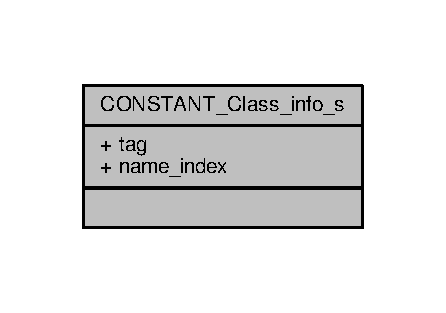
\includegraphics[width=214pt]{structCONSTANT__Class__info__s__coll__graph}
\end{center}
\end{figure}
\subsection*{Public Attributes}
\begin{DoxyCompactItemize}
\item 
\hyperlink{structs_8hpp_a17947ec3f3c1f2392eabd36c1ba5fec6}{cp\+\_\+tag} \hyperlink{structCONSTANT__Class__info__s_ae27fd46fb88a7d58404f0d0b29babc3e}{tag}
\item 
uint16\+\_\+t \hyperlink{structCONSTANT__Class__info__s_a3e852021d398529ee470dc916998fa6a}{name\+\_\+index}
\end{DoxyCompactItemize}


\subsection{Member Data Documentation}
\hypertarget{structCONSTANT__Class__info__s_a3e852021d398529ee470dc916998fa6a}{\index{C\+O\+N\+S\+T\+A\+N\+T\+\_\+\+Class\+\_\+info\+\_\+s@{C\+O\+N\+S\+T\+A\+N\+T\+\_\+\+Class\+\_\+info\+\_\+s}!name\+\_\+index@{name\+\_\+index}}
\index{name\+\_\+index@{name\+\_\+index}!C\+O\+N\+S\+T\+A\+N\+T\+\_\+\+Class\+\_\+info\+\_\+s@{C\+O\+N\+S\+T\+A\+N\+T\+\_\+\+Class\+\_\+info\+\_\+s}}
\subsubsection[{name\+\_\+index}]{\setlength{\rightskip}{0pt plus 5cm}uint16\+\_\+t C\+O\+N\+S\+T\+A\+N\+T\+\_\+\+Class\+\_\+info\+\_\+s\+::name\+\_\+index}}\label{structCONSTANT__Class__info__s_a3e852021d398529ee470dc916998fa6a}
\hypertarget{structCONSTANT__Class__info__s_ae27fd46fb88a7d58404f0d0b29babc3e}{\index{C\+O\+N\+S\+T\+A\+N\+T\+\_\+\+Class\+\_\+info\+\_\+s@{C\+O\+N\+S\+T\+A\+N\+T\+\_\+\+Class\+\_\+info\+\_\+s}!tag@{tag}}
\index{tag@{tag}!C\+O\+N\+S\+T\+A\+N\+T\+\_\+\+Class\+\_\+info\+\_\+s@{C\+O\+N\+S\+T\+A\+N\+T\+\_\+\+Class\+\_\+info\+\_\+s}}
\subsubsection[{tag}]{\setlength{\rightskip}{0pt plus 5cm}{\bf cp\+\_\+tag} C\+O\+N\+S\+T\+A\+N\+T\+\_\+\+Class\+\_\+info\+\_\+s\+::tag}}\label{structCONSTANT__Class__info__s_ae27fd46fb88a7d58404f0d0b29babc3e}


The documentation for this struct was generated from the following file\+:\begin{DoxyCompactItemize}
\item 
include/\hyperlink{structs_8hpp}{structs.\+hpp}\end{DoxyCompactItemize}

\hypertarget{structCONSTANT__Double__info__s}{\section{C\+O\+N\+S\+T\+A\+N\+T\+\_\+\+Double\+\_\+info\+\_\+s Struct Reference}
\label{structCONSTANT__Double__info__s}\index{C\+O\+N\+S\+T\+A\+N\+T\+\_\+\+Double\+\_\+info\+\_\+s@{C\+O\+N\+S\+T\+A\+N\+T\+\_\+\+Double\+\_\+info\+\_\+s}}
}


{\ttfamily \#include $<$structs.\+hpp$>$}



Collaboration diagram for C\+O\+N\+S\+T\+A\+N\+T\+\_\+\+Double\+\_\+info\+\_\+s\+:\nopagebreak
\begin{figure}[H]
\begin{center}
\leavevmode
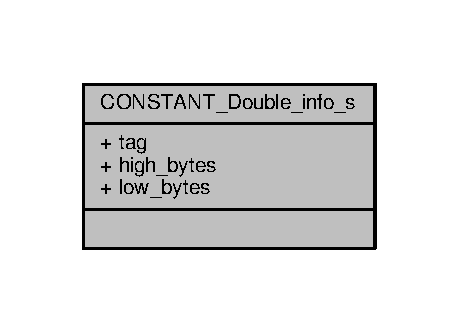
\includegraphics[width=220pt]{structCONSTANT__Double__info__s__coll__graph}
\end{center}
\end{figure}
\subsection*{Public Attributes}
\begin{DoxyCompactItemize}
\item 
\hyperlink{structs_8hpp_a17947ec3f3c1f2392eabd36c1ba5fec6}{cp\+\_\+tag} \hyperlink{structCONSTANT__Double__info__s_ac95905e32467bd7084ab69661f85dc83}{tag}
\item 
uint32\+\_\+t \hyperlink{structCONSTANT__Double__info__s_ac924312805777fa64c8f353464cc84fe}{high\+\_\+bytes}
\item 
uint32\+\_\+t \hyperlink{structCONSTANT__Double__info__s_ab4ea9f49f1751d71959cc7075c414cf3}{low\+\_\+bytes}
\end{DoxyCompactItemize}


\subsection{Member Data Documentation}
\hypertarget{structCONSTANT__Double__info__s_ac924312805777fa64c8f353464cc84fe}{\index{C\+O\+N\+S\+T\+A\+N\+T\+\_\+\+Double\+\_\+info\+\_\+s@{C\+O\+N\+S\+T\+A\+N\+T\+\_\+\+Double\+\_\+info\+\_\+s}!high\+\_\+bytes@{high\+\_\+bytes}}
\index{high\+\_\+bytes@{high\+\_\+bytes}!C\+O\+N\+S\+T\+A\+N\+T\+\_\+\+Double\+\_\+info\+\_\+s@{C\+O\+N\+S\+T\+A\+N\+T\+\_\+\+Double\+\_\+info\+\_\+s}}
\subsubsection[{high\+\_\+bytes}]{\setlength{\rightskip}{0pt plus 5cm}uint32\+\_\+t C\+O\+N\+S\+T\+A\+N\+T\+\_\+\+Double\+\_\+info\+\_\+s\+::high\+\_\+bytes}}\label{structCONSTANT__Double__info__s_ac924312805777fa64c8f353464cc84fe}
\hypertarget{structCONSTANT__Double__info__s_ab4ea9f49f1751d71959cc7075c414cf3}{\index{C\+O\+N\+S\+T\+A\+N\+T\+\_\+\+Double\+\_\+info\+\_\+s@{C\+O\+N\+S\+T\+A\+N\+T\+\_\+\+Double\+\_\+info\+\_\+s}!low\+\_\+bytes@{low\+\_\+bytes}}
\index{low\+\_\+bytes@{low\+\_\+bytes}!C\+O\+N\+S\+T\+A\+N\+T\+\_\+\+Double\+\_\+info\+\_\+s@{C\+O\+N\+S\+T\+A\+N\+T\+\_\+\+Double\+\_\+info\+\_\+s}}
\subsubsection[{low\+\_\+bytes}]{\setlength{\rightskip}{0pt plus 5cm}uint32\+\_\+t C\+O\+N\+S\+T\+A\+N\+T\+\_\+\+Double\+\_\+info\+\_\+s\+::low\+\_\+bytes}}\label{structCONSTANT__Double__info__s_ab4ea9f49f1751d71959cc7075c414cf3}
\hypertarget{structCONSTANT__Double__info__s_ac95905e32467bd7084ab69661f85dc83}{\index{C\+O\+N\+S\+T\+A\+N\+T\+\_\+\+Double\+\_\+info\+\_\+s@{C\+O\+N\+S\+T\+A\+N\+T\+\_\+\+Double\+\_\+info\+\_\+s}!tag@{tag}}
\index{tag@{tag}!C\+O\+N\+S\+T\+A\+N\+T\+\_\+\+Double\+\_\+info\+\_\+s@{C\+O\+N\+S\+T\+A\+N\+T\+\_\+\+Double\+\_\+info\+\_\+s}}
\subsubsection[{tag}]{\setlength{\rightskip}{0pt plus 5cm}{\bf cp\+\_\+tag} C\+O\+N\+S\+T\+A\+N\+T\+\_\+\+Double\+\_\+info\+\_\+s\+::tag}}\label{structCONSTANT__Double__info__s_ac95905e32467bd7084ab69661f85dc83}


The documentation for this struct was generated from the following file\+:\begin{DoxyCompactItemize}
\item 
include/\hyperlink{structs_8hpp}{structs.\+hpp}\end{DoxyCompactItemize}

\hypertarget{structCONSTANT__Fieldref__info__s}{\section{C\+O\+N\+S\+T\+A\+N\+T\+\_\+\+Fieldref\+\_\+info\+\_\+s Struct Reference}
\label{structCONSTANT__Fieldref__info__s}\index{C\+O\+N\+S\+T\+A\+N\+T\+\_\+\+Fieldref\+\_\+info\+\_\+s@{C\+O\+N\+S\+T\+A\+N\+T\+\_\+\+Fieldref\+\_\+info\+\_\+s}}
}


{\ttfamily \#include $<$structs.\+hpp$>$}



Collaboration diagram for C\+O\+N\+S\+T\+A\+N\+T\+\_\+\+Fieldref\+\_\+info\+\_\+s\+:\nopagebreak
\begin{figure}[H]
\begin{center}
\leavevmode
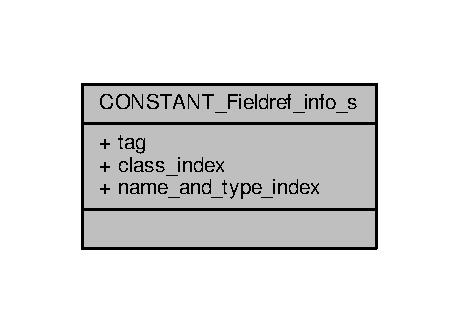
\includegraphics[width=220pt]{structCONSTANT__Fieldref__info__s__coll__graph}
\end{center}
\end{figure}
\subsection*{Public Attributes}
\begin{DoxyCompactItemize}
\item 
\hyperlink{structs_8hpp_a17947ec3f3c1f2392eabd36c1ba5fec6}{cp\+\_\+tag} \hyperlink{structCONSTANT__Fieldref__info__s_a87c470bc8260141489d7bde228887b2a}{tag}
\item 
uint16\+\_\+t \hyperlink{structCONSTANT__Fieldref__info__s_a43b294af041ee1cdb3bc276d0d51ffb9}{class\+\_\+index}
\item 
uint16\+\_\+t \hyperlink{structCONSTANT__Fieldref__info__s_a4577ca33395c8758c345b6e0a0fbc99b}{name\+\_\+and\+\_\+type\+\_\+index}
\end{DoxyCompactItemize}


\subsection{Member Data Documentation}
\hypertarget{structCONSTANT__Fieldref__info__s_a43b294af041ee1cdb3bc276d0d51ffb9}{\index{C\+O\+N\+S\+T\+A\+N\+T\+\_\+\+Fieldref\+\_\+info\+\_\+s@{C\+O\+N\+S\+T\+A\+N\+T\+\_\+\+Fieldref\+\_\+info\+\_\+s}!class\+\_\+index@{class\+\_\+index}}
\index{class\+\_\+index@{class\+\_\+index}!C\+O\+N\+S\+T\+A\+N\+T\+\_\+\+Fieldref\+\_\+info\+\_\+s@{C\+O\+N\+S\+T\+A\+N\+T\+\_\+\+Fieldref\+\_\+info\+\_\+s}}
\subsubsection[{class\+\_\+index}]{\setlength{\rightskip}{0pt plus 5cm}uint16\+\_\+t C\+O\+N\+S\+T\+A\+N\+T\+\_\+\+Fieldref\+\_\+info\+\_\+s\+::class\+\_\+index}}\label{structCONSTANT__Fieldref__info__s_a43b294af041ee1cdb3bc276d0d51ffb9}
\hypertarget{structCONSTANT__Fieldref__info__s_a4577ca33395c8758c345b6e0a0fbc99b}{\index{C\+O\+N\+S\+T\+A\+N\+T\+\_\+\+Fieldref\+\_\+info\+\_\+s@{C\+O\+N\+S\+T\+A\+N\+T\+\_\+\+Fieldref\+\_\+info\+\_\+s}!name\+\_\+and\+\_\+type\+\_\+index@{name\+\_\+and\+\_\+type\+\_\+index}}
\index{name\+\_\+and\+\_\+type\+\_\+index@{name\+\_\+and\+\_\+type\+\_\+index}!C\+O\+N\+S\+T\+A\+N\+T\+\_\+\+Fieldref\+\_\+info\+\_\+s@{C\+O\+N\+S\+T\+A\+N\+T\+\_\+\+Fieldref\+\_\+info\+\_\+s}}
\subsubsection[{name\+\_\+and\+\_\+type\+\_\+index}]{\setlength{\rightskip}{0pt plus 5cm}uint16\+\_\+t C\+O\+N\+S\+T\+A\+N\+T\+\_\+\+Fieldref\+\_\+info\+\_\+s\+::name\+\_\+and\+\_\+type\+\_\+index}}\label{structCONSTANT__Fieldref__info__s_a4577ca33395c8758c345b6e0a0fbc99b}
\hypertarget{structCONSTANT__Fieldref__info__s_a87c470bc8260141489d7bde228887b2a}{\index{C\+O\+N\+S\+T\+A\+N\+T\+\_\+\+Fieldref\+\_\+info\+\_\+s@{C\+O\+N\+S\+T\+A\+N\+T\+\_\+\+Fieldref\+\_\+info\+\_\+s}!tag@{tag}}
\index{tag@{tag}!C\+O\+N\+S\+T\+A\+N\+T\+\_\+\+Fieldref\+\_\+info\+\_\+s@{C\+O\+N\+S\+T\+A\+N\+T\+\_\+\+Fieldref\+\_\+info\+\_\+s}}
\subsubsection[{tag}]{\setlength{\rightskip}{0pt plus 5cm}{\bf cp\+\_\+tag} C\+O\+N\+S\+T\+A\+N\+T\+\_\+\+Fieldref\+\_\+info\+\_\+s\+::tag}}\label{structCONSTANT__Fieldref__info__s_a87c470bc8260141489d7bde228887b2a}


The documentation for this struct was generated from the following file\+:\begin{DoxyCompactItemize}
\item 
include/\hyperlink{structs_8hpp}{structs.\+hpp}\end{DoxyCompactItemize}

\hypertarget{structCONSTANT__Float__info__s}{\section{C\+O\+N\+S\+T\+A\+N\+T\+\_\+\+Float\+\_\+info\+\_\+s Struct Reference}
\label{structCONSTANT__Float__info__s}\index{C\+O\+N\+S\+T\+A\+N\+T\+\_\+\+Float\+\_\+info\+\_\+s@{C\+O\+N\+S\+T\+A\+N\+T\+\_\+\+Float\+\_\+info\+\_\+s}}
}


{\ttfamily \#include $<$structs.\+hpp$>$}



Collaboration diagram for C\+O\+N\+S\+T\+A\+N\+T\+\_\+\+Float\+\_\+info\+\_\+s\+:\nopagebreak
\begin{figure}[H]
\begin{center}
\leavevmode
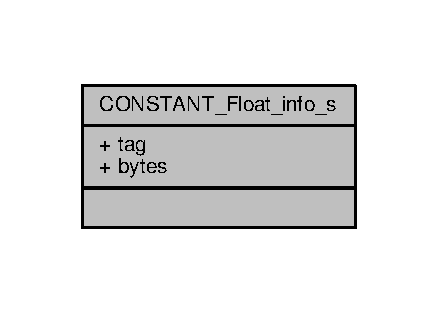
\includegraphics[width=210pt]{structCONSTANT__Float__info__s__coll__graph}
\end{center}
\end{figure}
\subsection*{Public Attributes}
\begin{DoxyCompactItemize}
\item 
\hyperlink{structs_8hpp_a17947ec3f3c1f2392eabd36c1ba5fec6}{cp\+\_\+tag} \hyperlink{structCONSTANT__Float__info__s_a478b54b29def2238db495fd72bd2c983}{tag}
\item 
uint32\+\_\+t \hyperlink{structCONSTANT__Float__info__s_a8055082e9793f98ddd1feb21029262c6}{bytes}
\end{DoxyCompactItemize}


\subsection{Member Data Documentation}
\hypertarget{structCONSTANT__Float__info__s_a8055082e9793f98ddd1feb21029262c6}{\index{C\+O\+N\+S\+T\+A\+N\+T\+\_\+\+Float\+\_\+info\+\_\+s@{C\+O\+N\+S\+T\+A\+N\+T\+\_\+\+Float\+\_\+info\+\_\+s}!bytes@{bytes}}
\index{bytes@{bytes}!C\+O\+N\+S\+T\+A\+N\+T\+\_\+\+Float\+\_\+info\+\_\+s@{C\+O\+N\+S\+T\+A\+N\+T\+\_\+\+Float\+\_\+info\+\_\+s}}
\subsubsection[{bytes}]{\setlength{\rightskip}{0pt plus 5cm}uint32\+\_\+t C\+O\+N\+S\+T\+A\+N\+T\+\_\+\+Float\+\_\+info\+\_\+s\+::bytes}}\label{structCONSTANT__Float__info__s_a8055082e9793f98ddd1feb21029262c6}
\hypertarget{structCONSTANT__Float__info__s_a478b54b29def2238db495fd72bd2c983}{\index{C\+O\+N\+S\+T\+A\+N\+T\+\_\+\+Float\+\_\+info\+\_\+s@{C\+O\+N\+S\+T\+A\+N\+T\+\_\+\+Float\+\_\+info\+\_\+s}!tag@{tag}}
\index{tag@{tag}!C\+O\+N\+S\+T\+A\+N\+T\+\_\+\+Float\+\_\+info\+\_\+s@{C\+O\+N\+S\+T\+A\+N\+T\+\_\+\+Float\+\_\+info\+\_\+s}}
\subsubsection[{tag}]{\setlength{\rightskip}{0pt plus 5cm}{\bf cp\+\_\+tag} C\+O\+N\+S\+T\+A\+N\+T\+\_\+\+Float\+\_\+info\+\_\+s\+::tag}}\label{structCONSTANT__Float__info__s_a478b54b29def2238db495fd72bd2c983}


The documentation for this struct was generated from the following file\+:\begin{DoxyCompactItemize}
\item 
include/\hyperlink{structs_8hpp}{structs.\+hpp}\end{DoxyCompactItemize}

\hypertarget{structCONSTANT__Integer__info__s}{\section{C\+O\+N\+S\+T\+A\+N\+T\+\_\+\+Integer\+\_\+info\+\_\+s Struct Reference}
\label{structCONSTANT__Integer__info__s}\index{C\+O\+N\+S\+T\+A\+N\+T\+\_\+\+Integer\+\_\+info\+\_\+s@{C\+O\+N\+S\+T\+A\+N\+T\+\_\+\+Integer\+\_\+info\+\_\+s}}
}


{\ttfamily \#include $<$structs.\+hpp$>$}



Collaboration diagram for C\+O\+N\+S\+T\+A\+N\+T\+\_\+\+Integer\+\_\+info\+\_\+s\+:\nopagebreak
\begin{figure}[H]
\begin{center}
\leavevmode
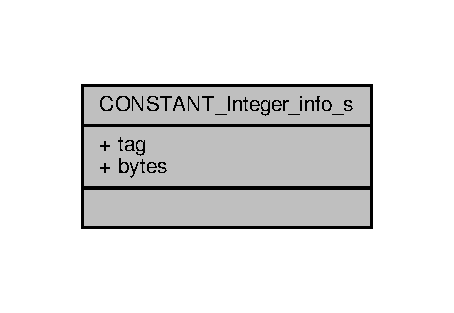
\includegraphics[width=218pt]{structCONSTANT__Integer__info__s__coll__graph}
\end{center}
\end{figure}
\subsection*{Public Attributes}
\begin{DoxyCompactItemize}
\item 
\hyperlink{structs_8hpp_a17947ec3f3c1f2392eabd36c1ba5fec6}{cp\+\_\+tag} \hyperlink{structCONSTANT__Integer__info__s_ab64157620cc3546f13d041e230280fb9}{tag}
\item 
uint32\+\_\+t \hyperlink{structCONSTANT__Integer__info__s_adf82e6a8faf5fd5f2dbb063e4d30edf7}{bytes}
\end{DoxyCompactItemize}


\subsection{Member Data Documentation}
\hypertarget{structCONSTANT__Integer__info__s_adf82e6a8faf5fd5f2dbb063e4d30edf7}{\index{C\+O\+N\+S\+T\+A\+N\+T\+\_\+\+Integer\+\_\+info\+\_\+s@{C\+O\+N\+S\+T\+A\+N\+T\+\_\+\+Integer\+\_\+info\+\_\+s}!bytes@{bytes}}
\index{bytes@{bytes}!C\+O\+N\+S\+T\+A\+N\+T\+\_\+\+Integer\+\_\+info\+\_\+s@{C\+O\+N\+S\+T\+A\+N\+T\+\_\+\+Integer\+\_\+info\+\_\+s}}
\subsubsection[{bytes}]{\setlength{\rightskip}{0pt plus 5cm}uint32\+\_\+t C\+O\+N\+S\+T\+A\+N\+T\+\_\+\+Integer\+\_\+info\+\_\+s\+::bytes}}\label{structCONSTANT__Integer__info__s_adf82e6a8faf5fd5f2dbb063e4d30edf7}
\hypertarget{structCONSTANT__Integer__info__s_ab64157620cc3546f13d041e230280fb9}{\index{C\+O\+N\+S\+T\+A\+N\+T\+\_\+\+Integer\+\_\+info\+\_\+s@{C\+O\+N\+S\+T\+A\+N\+T\+\_\+\+Integer\+\_\+info\+\_\+s}!tag@{tag}}
\index{tag@{tag}!C\+O\+N\+S\+T\+A\+N\+T\+\_\+\+Integer\+\_\+info\+\_\+s@{C\+O\+N\+S\+T\+A\+N\+T\+\_\+\+Integer\+\_\+info\+\_\+s}}
\subsubsection[{tag}]{\setlength{\rightskip}{0pt plus 5cm}{\bf cp\+\_\+tag} C\+O\+N\+S\+T\+A\+N\+T\+\_\+\+Integer\+\_\+info\+\_\+s\+::tag}}\label{structCONSTANT__Integer__info__s_ab64157620cc3546f13d041e230280fb9}


The documentation for this struct was generated from the following file\+:\begin{DoxyCompactItemize}
\item 
include/\hyperlink{structs_8hpp}{structs.\+hpp}\end{DoxyCompactItemize}

\hypertarget{structCONSTANT__InterfaceMethodref__info__s}{\section{C\+O\+N\+S\+T\+A\+N\+T\+\_\+\+Interface\+Methodref\+\_\+info\+\_\+s Struct Reference}
\label{structCONSTANT__InterfaceMethodref__info__s}\index{C\+O\+N\+S\+T\+A\+N\+T\+\_\+\+Interface\+Methodref\+\_\+info\+\_\+s@{C\+O\+N\+S\+T\+A\+N\+T\+\_\+\+Interface\+Methodref\+\_\+info\+\_\+s}}
}


{\ttfamily \#include $<$structs.\+hpp$>$}



Collaboration diagram for C\+O\+N\+S\+T\+A\+N\+T\+\_\+\+Interface\+Methodref\+\_\+info\+\_\+s\+:\nopagebreak
\begin{figure}[H]
\begin{center}
\leavevmode
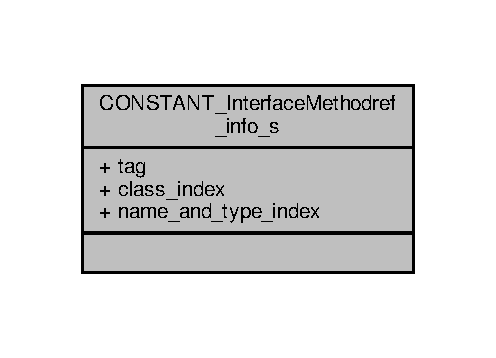
\includegraphics[width=238pt]{structCONSTANT__InterfaceMethodref__info__s__coll__graph}
\end{center}
\end{figure}
\subsection*{Public Attributes}
\begin{DoxyCompactItemize}
\item 
\hyperlink{structs_8hpp_a17947ec3f3c1f2392eabd36c1ba5fec6}{cp\+\_\+tag} \hyperlink{structCONSTANT__InterfaceMethodref__info__s_a11c19f84f330597406b300345686e89d}{tag}
\item 
uint16\+\_\+t \hyperlink{structCONSTANT__InterfaceMethodref__info__s_abc7d8e3373d4b57beb8c4a6c11783fb3}{class\+\_\+index}
\item 
uint16\+\_\+t \hyperlink{structCONSTANT__InterfaceMethodref__info__s_a11922bbce7b46f1f2bdc91e544335ef1}{name\+\_\+and\+\_\+type\+\_\+index}
\end{DoxyCompactItemize}


\subsection{Member Data Documentation}
\hypertarget{structCONSTANT__InterfaceMethodref__info__s_abc7d8e3373d4b57beb8c4a6c11783fb3}{\index{C\+O\+N\+S\+T\+A\+N\+T\+\_\+\+Interface\+Methodref\+\_\+info\+\_\+s@{C\+O\+N\+S\+T\+A\+N\+T\+\_\+\+Interface\+Methodref\+\_\+info\+\_\+s}!class\+\_\+index@{class\+\_\+index}}
\index{class\+\_\+index@{class\+\_\+index}!C\+O\+N\+S\+T\+A\+N\+T\+\_\+\+Interface\+Methodref\+\_\+info\+\_\+s@{C\+O\+N\+S\+T\+A\+N\+T\+\_\+\+Interface\+Methodref\+\_\+info\+\_\+s}}
\subsubsection[{class\+\_\+index}]{\setlength{\rightskip}{0pt plus 5cm}uint16\+\_\+t C\+O\+N\+S\+T\+A\+N\+T\+\_\+\+Interface\+Methodref\+\_\+info\+\_\+s\+::class\+\_\+index}}\label{structCONSTANT__InterfaceMethodref__info__s_abc7d8e3373d4b57beb8c4a6c11783fb3}
\hypertarget{structCONSTANT__InterfaceMethodref__info__s_a11922bbce7b46f1f2bdc91e544335ef1}{\index{C\+O\+N\+S\+T\+A\+N\+T\+\_\+\+Interface\+Methodref\+\_\+info\+\_\+s@{C\+O\+N\+S\+T\+A\+N\+T\+\_\+\+Interface\+Methodref\+\_\+info\+\_\+s}!name\+\_\+and\+\_\+type\+\_\+index@{name\+\_\+and\+\_\+type\+\_\+index}}
\index{name\+\_\+and\+\_\+type\+\_\+index@{name\+\_\+and\+\_\+type\+\_\+index}!C\+O\+N\+S\+T\+A\+N\+T\+\_\+\+Interface\+Methodref\+\_\+info\+\_\+s@{C\+O\+N\+S\+T\+A\+N\+T\+\_\+\+Interface\+Methodref\+\_\+info\+\_\+s}}
\subsubsection[{name\+\_\+and\+\_\+type\+\_\+index}]{\setlength{\rightskip}{0pt plus 5cm}uint16\+\_\+t C\+O\+N\+S\+T\+A\+N\+T\+\_\+\+Interface\+Methodref\+\_\+info\+\_\+s\+::name\+\_\+and\+\_\+type\+\_\+index}}\label{structCONSTANT__InterfaceMethodref__info__s_a11922bbce7b46f1f2bdc91e544335ef1}
\hypertarget{structCONSTANT__InterfaceMethodref__info__s_a11c19f84f330597406b300345686e89d}{\index{C\+O\+N\+S\+T\+A\+N\+T\+\_\+\+Interface\+Methodref\+\_\+info\+\_\+s@{C\+O\+N\+S\+T\+A\+N\+T\+\_\+\+Interface\+Methodref\+\_\+info\+\_\+s}!tag@{tag}}
\index{tag@{tag}!C\+O\+N\+S\+T\+A\+N\+T\+\_\+\+Interface\+Methodref\+\_\+info\+\_\+s@{C\+O\+N\+S\+T\+A\+N\+T\+\_\+\+Interface\+Methodref\+\_\+info\+\_\+s}}
\subsubsection[{tag}]{\setlength{\rightskip}{0pt plus 5cm}{\bf cp\+\_\+tag} C\+O\+N\+S\+T\+A\+N\+T\+\_\+\+Interface\+Methodref\+\_\+info\+\_\+s\+::tag}}\label{structCONSTANT__InterfaceMethodref__info__s_a11c19f84f330597406b300345686e89d}


The documentation for this struct was generated from the following file\+:\begin{DoxyCompactItemize}
\item 
include/\hyperlink{structs_8hpp}{structs.\+hpp}\end{DoxyCompactItemize}

\hypertarget{structCONSTANT__InvokeDynamic__info__s}{\section{C\+O\+N\+S\+T\+A\+N\+T\+\_\+\+Invoke\+Dynamic\+\_\+info\+\_\+s Struct Reference}
\label{structCONSTANT__InvokeDynamic__info__s}\index{C\+O\+N\+S\+T\+A\+N\+T\+\_\+\+Invoke\+Dynamic\+\_\+info\+\_\+s@{C\+O\+N\+S\+T\+A\+N\+T\+\_\+\+Invoke\+Dynamic\+\_\+info\+\_\+s}}
}


{\ttfamily \#include $<$structs.\+hpp$>$}



Collaboration diagram for C\+O\+N\+S\+T\+A\+N\+T\+\_\+\+Invoke\+Dynamic\+\_\+info\+\_\+s\+:\nopagebreak
\begin{figure}[H]
\begin{center}
\leavevmode
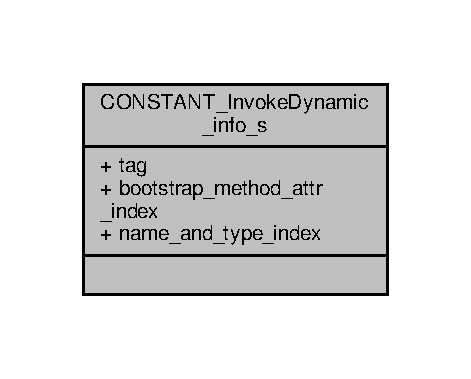
\includegraphics[width=226pt]{structCONSTANT__InvokeDynamic__info__s__coll__graph}
\end{center}
\end{figure}
\subsection*{Public Attributes}
\begin{DoxyCompactItemize}
\item 
\hyperlink{structs_8hpp_a17947ec3f3c1f2392eabd36c1ba5fec6}{cp\+\_\+tag} \hyperlink{structCONSTANT__InvokeDynamic__info__s_a8e871033bfc2900cb240926b90f76449}{tag}
\item 
uint16\+\_\+t \hyperlink{structCONSTANT__InvokeDynamic__info__s_a1729eda16857b6fe2c266fd101335cb7}{bootstrap\+\_\+method\+\_\+attr\+\_\+index}
\item 
uint16\+\_\+t \hyperlink{structCONSTANT__InvokeDynamic__info__s_a8498bc18f2a985a82998a5d4d255a614}{name\+\_\+and\+\_\+type\+\_\+index}
\end{DoxyCompactItemize}


\subsection{Member Data Documentation}
\hypertarget{structCONSTANT__InvokeDynamic__info__s_a1729eda16857b6fe2c266fd101335cb7}{\index{C\+O\+N\+S\+T\+A\+N\+T\+\_\+\+Invoke\+Dynamic\+\_\+info\+\_\+s@{C\+O\+N\+S\+T\+A\+N\+T\+\_\+\+Invoke\+Dynamic\+\_\+info\+\_\+s}!bootstrap\+\_\+method\+\_\+attr\+\_\+index@{bootstrap\+\_\+method\+\_\+attr\+\_\+index}}
\index{bootstrap\+\_\+method\+\_\+attr\+\_\+index@{bootstrap\+\_\+method\+\_\+attr\+\_\+index}!C\+O\+N\+S\+T\+A\+N\+T\+\_\+\+Invoke\+Dynamic\+\_\+info\+\_\+s@{C\+O\+N\+S\+T\+A\+N\+T\+\_\+\+Invoke\+Dynamic\+\_\+info\+\_\+s}}
\subsubsection[{bootstrap\+\_\+method\+\_\+attr\+\_\+index}]{\setlength{\rightskip}{0pt plus 5cm}uint16\+\_\+t C\+O\+N\+S\+T\+A\+N\+T\+\_\+\+Invoke\+Dynamic\+\_\+info\+\_\+s\+::bootstrap\+\_\+method\+\_\+attr\+\_\+index}}\label{structCONSTANT__InvokeDynamic__info__s_a1729eda16857b6fe2c266fd101335cb7}
\hypertarget{structCONSTANT__InvokeDynamic__info__s_a8498bc18f2a985a82998a5d4d255a614}{\index{C\+O\+N\+S\+T\+A\+N\+T\+\_\+\+Invoke\+Dynamic\+\_\+info\+\_\+s@{C\+O\+N\+S\+T\+A\+N\+T\+\_\+\+Invoke\+Dynamic\+\_\+info\+\_\+s}!name\+\_\+and\+\_\+type\+\_\+index@{name\+\_\+and\+\_\+type\+\_\+index}}
\index{name\+\_\+and\+\_\+type\+\_\+index@{name\+\_\+and\+\_\+type\+\_\+index}!C\+O\+N\+S\+T\+A\+N\+T\+\_\+\+Invoke\+Dynamic\+\_\+info\+\_\+s@{C\+O\+N\+S\+T\+A\+N\+T\+\_\+\+Invoke\+Dynamic\+\_\+info\+\_\+s}}
\subsubsection[{name\+\_\+and\+\_\+type\+\_\+index}]{\setlength{\rightskip}{0pt plus 5cm}uint16\+\_\+t C\+O\+N\+S\+T\+A\+N\+T\+\_\+\+Invoke\+Dynamic\+\_\+info\+\_\+s\+::name\+\_\+and\+\_\+type\+\_\+index}}\label{structCONSTANT__InvokeDynamic__info__s_a8498bc18f2a985a82998a5d4d255a614}
\hypertarget{structCONSTANT__InvokeDynamic__info__s_a8e871033bfc2900cb240926b90f76449}{\index{C\+O\+N\+S\+T\+A\+N\+T\+\_\+\+Invoke\+Dynamic\+\_\+info\+\_\+s@{C\+O\+N\+S\+T\+A\+N\+T\+\_\+\+Invoke\+Dynamic\+\_\+info\+\_\+s}!tag@{tag}}
\index{tag@{tag}!C\+O\+N\+S\+T\+A\+N\+T\+\_\+\+Invoke\+Dynamic\+\_\+info\+\_\+s@{C\+O\+N\+S\+T\+A\+N\+T\+\_\+\+Invoke\+Dynamic\+\_\+info\+\_\+s}}
\subsubsection[{tag}]{\setlength{\rightskip}{0pt plus 5cm}{\bf cp\+\_\+tag} C\+O\+N\+S\+T\+A\+N\+T\+\_\+\+Invoke\+Dynamic\+\_\+info\+\_\+s\+::tag}}\label{structCONSTANT__InvokeDynamic__info__s_a8e871033bfc2900cb240926b90f76449}


The documentation for this struct was generated from the following file\+:\begin{DoxyCompactItemize}
\item 
include/\hyperlink{structs_8hpp}{structs.\+hpp}\end{DoxyCompactItemize}

\hypertarget{structCONSTANT__Long__info__s}{\section{C\+O\+N\+S\+T\+A\+N\+T\+\_\+\+Long\+\_\+info\+\_\+s Struct Reference}
\label{structCONSTANT__Long__info__s}\index{C\+O\+N\+S\+T\+A\+N\+T\+\_\+\+Long\+\_\+info\+\_\+s@{C\+O\+N\+S\+T\+A\+N\+T\+\_\+\+Long\+\_\+info\+\_\+s}}
}


{\ttfamily \#include $<$structs.\+hpp$>$}



Collaboration diagram for C\+O\+N\+S\+T\+A\+N\+T\+\_\+\+Long\+\_\+info\+\_\+s\+:\nopagebreak
\begin{figure}[H]
\begin{center}
\leavevmode
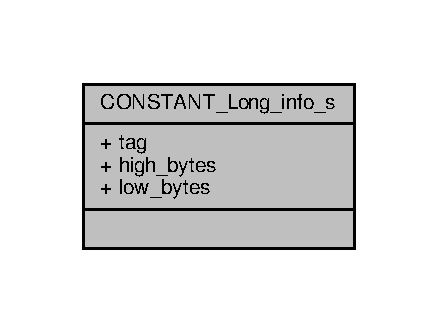
\includegraphics[width=210pt]{structCONSTANT__Long__info__s__coll__graph}
\end{center}
\end{figure}
\subsection*{Public Attributes}
\begin{DoxyCompactItemize}
\item 
\hyperlink{structs_8hpp_a17947ec3f3c1f2392eabd36c1ba5fec6}{cp\+\_\+tag} \hyperlink{structCONSTANT__Long__info__s_abdc4201e4bf9eac8c7d632983cccedd3}{tag}
\item 
uint32\+\_\+t \hyperlink{structCONSTANT__Long__info__s_ae75d18eb47743d41d6a12698a0a9919e}{high\+\_\+bytes}
\item 
uint32\+\_\+t \hyperlink{structCONSTANT__Long__info__s_a221f2f424e3fcec977b0375a1ce1986b}{low\+\_\+bytes}
\end{DoxyCompactItemize}


\subsection{Member Data Documentation}
\hypertarget{structCONSTANT__Long__info__s_ae75d18eb47743d41d6a12698a0a9919e}{\index{C\+O\+N\+S\+T\+A\+N\+T\+\_\+\+Long\+\_\+info\+\_\+s@{C\+O\+N\+S\+T\+A\+N\+T\+\_\+\+Long\+\_\+info\+\_\+s}!high\+\_\+bytes@{high\+\_\+bytes}}
\index{high\+\_\+bytes@{high\+\_\+bytes}!C\+O\+N\+S\+T\+A\+N\+T\+\_\+\+Long\+\_\+info\+\_\+s@{C\+O\+N\+S\+T\+A\+N\+T\+\_\+\+Long\+\_\+info\+\_\+s}}
\subsubsection[{high\+\_\+bytes}]{\setlength{\rightskip}{0pt plus 5cm}uint32\+\_\+t C\+O\+N\+S\+T\+A\+N\+T\+\_\+\+Long\+\_\+info\+\_\+s\+::high\+\_\+bytes}}\label{structCONSTANT__Long__info__s_ae75d18eb47743d41d6a12698a0a9919e}
\hypertarget{structCONSTANT__Long__info__s_a221f2f424e3fcec977b0375a1ce1986b}{\index{C\+O\+N\+S\+T\+A\+N\+T\+\_\+\+Long\+\_\+info\+\_\+s@{C\+O\+N\+S\+T\+A\+N\+T\+\_\+\+Long\+\_\+info\+\_\+s}!low\+\_\+bytes@{low\+\_\+bytes}}
\index{low\+\_\+bytes@{low\+\_\+bytes}!C\+O\+N\+S\+T\+A\+N\+T\+\_\+\+Long\+\_\+info\+\_\+s@{C\+O\+N\+S\+T\+A\+N\+T\+\_\+\+Long\+\_\+info\+\_\+s}}
\subsubsection[{low\+\_\+bytes}]{\setlength{\rightskip}{0pt plus 5cm}uint32\+\_\+t C\+O\+N\+S\+T\+A\+N\+T\+\_\+\+Long\+\_\+info\+\_\+s\+::low\+\_\+bytes}}\label{structCONSTANT__Long__info__s_a221f2f424e3fcec977b0375a1ce1986b}
\hypertarget{structCONSTANT__Long__info__s_abdc4201e4bf9eac8c7d632983cccedd3}{\index{C\+O\+N\+S\+T\+A\+N\+T\+\_\+\+Long\+\_\+info\+\_\+s@{C\+O\+N\+S\+T\+A\+N\+T\+\_\+\+Long\+\_\+info\+\_\+s}!tag@{tag}}
\index{tag@{tag}!C\+O\+N\+S\+T\+A\+N\+T\+\_\+\+Long\+\_\+info\+\_\+s@{C\+O\+N\+S\+T\+A\+N\+T\+\_\+\+Long\+\_\+info\+\_\+s}}
\subsubsection[{tag}]{\setlength{\rightskip}{0pt plus 5cm}{\bf cp\+\_\+tag} C\+O\+N\+S\+T\+A\+N\+T\+\_\+\+Long\+\_\+info\+\_\+s\+::tag}}\label{structCONSTANT__Long__info__s_abdc4201e4bf9eac8c7d632983cccedd3}


The documentation for this struct was generated from the following file\+:\begin{DoxyCompactItemize}
\item 
include/\hyperlink{structs_8hpp}{structs.\+hpp}\end{DoxyCompactItemize}

\hypertarget{structCONSTANT__MethodHandle__info__s}{\section{C\+O\+N\+S\+T\+A\+N\+T\+\_\+\+Method\+Handle\+\_\+info\+\_\+s Struct Reference}
\label{structCONSTANT__MethodHandle__info__s}\index{C\+O\+N\+S\+T\+A\+N\+T\+\_\+\+Method\+Handle\+\_\+info\+\_\+s@{C\+O\+N\+S\+T\+A\+N\+T\+\_\+\+Method\+Handle\+\_\+info\+\_\+s}}
}


{\ttfamily \#include $<$structs.\+hpp$>$}



Collaboration diagram for C\+O\+N\+S\+T\+A\+N\+T\+\_\+\+Method\+Handle\+\_\+info\+\_\+s\+:\nopagebreak
\begin{figure}[H]
\begin{center}
\leavevmode
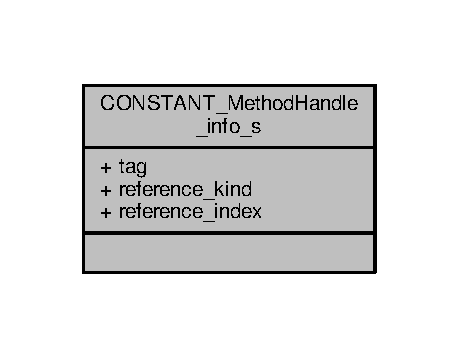
\includegraphics[width=220pt]{structCONSTANT__MethodHandle__info__s__coll__graph}
\end{center}
\end{figure}
\subsection*{Public Attributes}
\begin{DoxyCompactItemize}
\item 
\hyperlink{structs_8hpp_a17947ec3f3c1f2392eabd36c1ba5fec6}{cp\+\_\+tag} \hyperlink{structCONSTANT__MethodHandle__info__s_ac82e027678357e8dda9d759ea771848d}{tag}
\item 
uint8\+\_\+t \hyperlink{structCONSTANT__MethodHandle__info__s_a013248dcf4a680295f921041c203a51b}{reference\+\_\+kind}
\item 
uint16\+\_\+t \hyperlink{structCONSTANT__MethodHandle__info__s_a99ccde8a51c1a29e8b90816e11d36a0d}{reference\+\_\+index}
\end{DoxyCompactItemize}


\subsection{Member Data Documentation}
\hypertarget{structCONSTANT__MethodHandle__info__s_a99ccde8a51c1a29e8b90816e11d36a0d}{\index{C\+O\+N\+S\+T\+A\+N\+T\+\_\+\+Method\+Handle\+\_\+info\+\_\+s@{C\+O\+N\+S\+T\+A\+N\+T\+\_\+\+Method\+Handle\+\_\+info\+\_\+s}!reference\+\_\+index@{reference\+\_\+index}}
\index{reference\+\_\+index@{reference\+\_\+index}!C\+O\+N\+S\+T\+A\+N\+T\+\_\+\+Method\+Handle\+\_\+info\+\_\+s@{C\+O\+N\+S\+T\+A\+N\+T\+\_\+\+Method\+Handle\+\_\+info\+\_\+s}}
\subsubsection[{reference\+\_\+index}]{\setlength{\rightskip}{0pt plus 5cm}uint16\+\_\+t C\+O\+N\+S\+T\+A\+N\+T\+\_\+\+Method\+Handle\+\_\+info\+\_\+s\+::reference\+\_\+index}}\label{structCONSTANT__MethodHandle__info__s_a99ccde8a51c1a29e8b90816e11d36a0d}
\hypertarget{structCONSTANT__MethodHandle__info__s_a013248dcf4a680295f921041c203a51b}{\index{C\+O\+N\+S\+T\+A\+N\+T\+\_\+\+Method\+Handle\+\_\+info\+\_\+s@{C\+O\+N\+S\+T\+A\+N\+T\+\_\+\+Method\+Handle\+\_\+info\+\_\+s}!reference\+\_\+kind@{reference\+\_\+kind}}
\index{reference\+\_\+kind@{reference\+\_\+kind}!C\+O\+N\+S\+T\+A\+N\+T\+\_\+\+Method\+Handle\+\_\+info\+\_\+s@{C\+O\+N\+S\+T\+A\+N\+T\+\_\+\+Method\+Handle\+\_\+info\+\_\+s}}
\subsubsection[{reference\+\_\+kind}]{\setlength{\rightskip}{0pt plus 5cm}uint8\+\_\+t C\+O\+N\+S\+T\+A\+N\+T\+\_\+\+Method\+Handle\+\_\+info\+\_\+s\+::reference\+\_\+kind}}\label{structCONSTANT__MethodHandle__info__s_a013248dcf4a680295f921041c203a51b}
\hypertarget{structCONSTANT__MethodHandle__info__s_ac82e027678357e8dda9d759ea771848d}{\index{C\+O\+N\+S\+T\+A\+N\+T\+\_\+\+Method\+Handle\+\_\+info\+\_\+s@{C\+O\+N\+S\+T\+A\+N\+T\+\_\+\+Method\+Handle\+\_\+info\+\_\+s}!tag@{tag}}
\index{tag@{tag}!C\+O\+N\+S\+T\+A\+N\+T\+\_\+\+Method\+Handle\+\_\+info\+\_\+s@{C\+O\+N\+S\+T\+A\+N\+T\+\_\+\+Method\+Handle\+\_\+info\+\_\+s}}
\subsubsection[{tag}]{\setlength{\rightskip}{0pt plus 5cm}{\bf cp\+\_\+tag} C\+O\+N\+S\+T\+A\+N\+T\+\_\+\+Method\+Handle\+\_\+info\+\_\+s\+::tag}}\label{structCONSTANT__MethodHandle__info__s_ac82e027678357e8dda9d759ea771848d}


The documentation for this struct was generated from the following file\+:\begin{DoxyCompactItemize}
\item 
include/\hyperlink{structs_8hpp}{structs.\+hpp}\end{DoxyCompactItemize}

\hypertarget{structCONSTANT__Methodref__info__s}{\section{C\+O\+N\+S\+T\+A\+N\+T\+\_\+\+Methodref\+\_\+info\+\_\+s Struct Reference}
\label{structCONSTANT__Methodref__info__s}\index{C\+O\+N\+S\+T\+A\+N\+T\+\_\+\+Methodref\+\_\+info\+\_\+s@{C\+O\+N\+S\+T\+A\+N\+T\+\_\+\+Methodref\+\_\+info\+\_\+s}}
}


{\ttfamily \#include $<$structs.\+hpp$>$}



Collaboration diagram for C\+O\+N\+S\+T\+A\+N\+T\+\_\+\+Methodref\+\_\+info\+\_\+s\+:\nopagebreak
\begin{figure}[H]
\begin{center}
\leavevmode
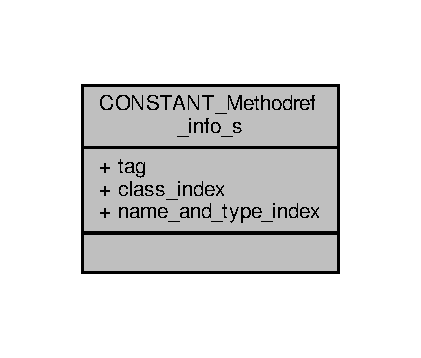
\includegraphics[width=202pt]{structCONSTANT__Methodref__info__s__coll__graph}
\end{center}
\end{figure}
\subsection*{Public Attributes}
\begin{DoxyCompactItemize}
\item 
\hyperlink{structs_8hpp_a17947ec3f3c1f2392eabd36c1ba5fec6}{cp\+\_\+tag} \hyperlink{structCONSTANT__Methodref__info__s_ac808580c07823c6e5413491b0b297a20}{tag}
\item 
uint16\+\_\+t \hyperlink{structCONSTANT__Methodref__info__s_a20509be0dbe4f181a490951022b76113}{class\+\_\+index}
\item 
uint16\+\_\+t \hyperlink{structCONSTANT__Methodref__info__s_ac669a727a4485e90f35bffd37888b7d2}{name\+\_\+and\+\_\+type\+\_\+index}
\end{DoxyCompactItemize}


\subsection{Member Data Documentation}
\hypertarget{structCONSTANT__Methodref__info__s_a20509be0dbe4f181a490951022b76113}{\index{C\+O\+N\+S\+T\+A\+N\+T\+\_\+\+Methodref\+\_\+info\+\_\+s@{C\+O\+N\+S\+T\+A\+N\+T\+\_\+\+Methodref\+\_\+info\+\_\+s}!class\+\_\+index@{class\+\_\+index}}
\index{class\+\_\+index@{class\+\_\+index}!C\+O\+N\+S\+T\+A\+N\+T\+\_\+\+Methodref\+\_\+info\+\_\+s@{C\+O\+N\+S\+T\+A\+N\+T\+\_\+\+Methodref\+\_\+info\+\_\+s}}
\subsubsection[{class\+\_\+index}]{\setlength{\rightskip}{0pt plus 5cm}uint16\+\_\+t C\+O\+N\+S\+T\+A\+N\+T\+\_\+\+Methodref\+\_\+info\+\_\+s\+::class\+\_\+index}}\label{structCONSTANT__Methodref__info__s_a20509be0dbe4f181a490951022b76113}
\hypertarget{structCONSTANT__Methodref__info__s_ac669a727a4485e90f35bffd37888b7d2}{\index{C\+O\+N\+S\+T\+A\+N\+T\+\_\+\+Methodref\+\_\+info\+\_\+s@{C\+O\+N\+S\+T\+A\+N\+T\+\_\+\+Methodref\+\_\+info\+\_\+s}!name\+\_\+and\+\_\+type\+\_\+index@{name\+\_\+and\+\_\+type\+\_\+index}}
\index{name\+\_\+and\+\_\+type\+\_\+index@{name\+\_\+and\+\_\+type\+\_\+index}!C\+O\+N\+S\+T\+A\+N\+T\+\_\+\+Methodref\+\_\+info\+\_\+s@{C\+O\+N\+S\+T\+A\+N\+T\+\_\+\+Methodref\+\_\+info\+\_\+s}}
\subsubsection[{name\+\_\+and\+\_\+type\+\_\+index}]{\setlength{\rightskip}{0pt plus 5cm}uint16\+\_\+t C\+O\+N\+S\+T\+A\+N\+T\+\_\+\+Methodref\+\_\+info\+\_\+s\+::name\+\_\+and\+\_\+type\+\_\+index}}\label{structCONSTANT__Methodref__info__s_ac669a727a4485e90f35bffd37888b7d2}
\hypertarget{structCONSTANT__Methodref__info__s_ac808580c07823c6e5413491b0b297a20}{\index{C\+O\+N\+S\+T\+A\+N\+T\+\_\+\+Methodref\+\_\+info\+\_\+s@{C\+O\+N\+S\+T\+A\+N\+T\+\_\+\+Methodref\+\_\+info\+\_\+s}!tag@{tag}}
\index{tag@{tag}!C\+O\+N\+S\+T\+A\+N\+T\+\_\+\+Methodref\+\_\+info\+\_\+s@{C\+O\+N\+S\+T\+A\+N\+T\+\_\+\+Methodref\+\_\+info\+\_\+s}}
\subsubsection[{tag}]{\setlength{\rightskip}{0pt plus 5cm}{\bf cp\+\_\+tag} C\+O\+N\+S\+T\+A\+N\+T\+\_\+\+Methodref\+\_\+info\+\_\+s\+::tag}}\label{structCONSTANT__Methodref__info__s_ac808580c07823c6e5413491b0b297a20}


The documentation for this struct was generated from the following file\+:\begin{DoxyCompactItemize}
\item 
include/\hyperlink{structs_8hpp}{structs.\+hpp}\end{DoxyCompactItemize}

\hypertarget{structCONSTANT__MethodType__info__s}{\section{C\+O\+N\+S\+T\+A\+N\+T\+\_\+\+Method\+Type\+\_\+info\+\_\+s Struct Reference}
\label{structCONSTANT__MethodType__info__s}\index{C\+O\+N\+S\+T\+A\+N\+T\+\_\+\+Method\+Type\+\_\+info\+\_\+s@{C\+O\+N\+S\+T\+A\+N\+T\+\_\+\+Method\+Type\+\_\+info\+\_\+s}}
}


{\ttfamily \#include $<$structs.\+hpp$>$}



Collaboration diagram for C\+O\+N\+S\+T\+A\+N\+T\+\_\+\+Method\+Type\+\_\+info\+\_\+s\+:\nopagebreak
\begin{figure}[H]
\begin{center}
\leavevmode
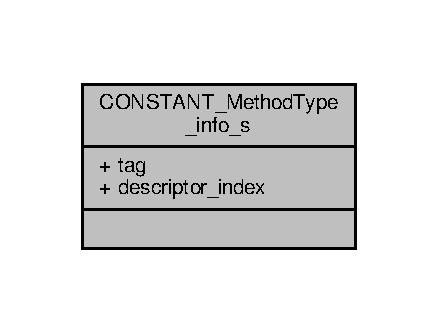
\includegraphics[width=210pt]{structCONSTANT__MethodType__info__s__coll__graph}
\end{center}
\end{figure}
\subsection*{Public Attributes}
\begin{DoxyCompactItemize}
\item 
\hyperlink{structs_8hpp_a17947ec3f3c1f2392eabd36c1ba5fec6}{cp\+\_\+tag} \hyperlink{structCONSTANT__MethodType__info__s_a0218ac52c1a8a8eebd94e09eda7949c6}{tag}
\item 
uint16\+\_\+t \hyperlink{structCONSTANT__MethodType__info__s_afb5f88f171fd11196c453eedceb70117}{descriptor\+\_\+index}
\end{DoxyCompactItemize}


\subsection{Member Data Documentation}
\hypertarget{structCONSTANT__MethodType__info__s_afb5f88f171fd11196c453eedceb70117}{\index{C\+O\+N\+S\+T\+A\+N\+T\+\_\+\+Method\+Type\+\_\+info\+\_\+s@{C\+O\+N\+S\+T\+A\+N\+T\+\_\+\+Method\+Type\+\_\+info\+\_\+s}!descriptor\+\_\+index@{descriptor\+\_\+index}}
\index{descriptor\+\_\+index@{descriptor\+\_\+index}!C\+O\+N\+S\+T\+A\+N\+T\+\_\+\+Method\+Type\+\_\+info\+\_\+s@{C\+O\+N\+S\+T\+A\+N\+T\+\_\+\+Method\+Type\+\_\+info\+\_\+s}}
\subsubsection[{descriptor\+\_\+index}]{\setlength{\rightskip}{0pt plus 5cm}uint16\+\_\+t C\+O\+N\+S\+T\+A\+N\+T\+\_\+\+Method\+Type\+\_\+info\+\_\+s\+::descriptor\+\_\+index}}\label{structCONSTANT__MethodType__info__s_afb5f88f171fd11196c453eedceb70117}
\hypertarget{structCONSTANT__MethodType__info__s_a0218ac52c1a8a8eebd94e09eda7949c6}{\index{C\+O\+N\+S\+T\+A\+N\+T\+\_\+\+Method\+Type\+\_\+info\+\_\+s@{C\+O\+N\+S\+T\+A\+N\+T\+\_\+\+Method\+Type\+\_\+info\+\_\+s}!tag@{tag}}
\index{tag@{tag}!C\+O\+N\+S\+T\+A\+N\+T\+\_\+\+Method\+Type\+\_\+info\+\_\+s@{C\+O\+N\+S\+T\+A\+N\+T\+\_\+\+Method\+Type\+\_\+info\+\_\+s}}
\subsubsection[{tag}]{\setlength{\rightskip}{0pt plus 5cm}{\bf cp\+\_\+tag} C\+O\+N\+S\+T\+A\+N\+T\+\_\+\+Method\+Type\+\_\+info\+\_\+s\+::tag}}\label{structCONSTANT__MethodType__info__s_a0218ac52c1a8a8eebd94e09eda7949c6}


The documentation for this struct was generated from the following file\+:\begin{DoxyCompactItemize}
\item 
include/\hyperlink{structs_8hpp}{structs.\+hpp}\end{DoxyCompactItemize}

\hypertarget{structCONSTANT__NameAndType__info__s}{\section{C\+O\+N\+S\+T\+A\+N\+T\+\_\+\+Name\+And\+Type\+\_\+info\+\_\+s Struct Reference}
\label{structCONSTANT__NameAndType__info__s}\index{C\+O\+N\+S\+T\+A\+N\+T\+\_\+\+Name\+And\+Type\+\_\+info\+\_\+s@{C\+O\+N\+S\+T\+A\+N\+T\+\_\+\+Name\+And\+Type\+\_\+info\+\_\+s}}
}


{\ttfamily \#include $<$structs.\+hpp$>$}



Collaboration diagram for C\+O\+N\+S\+T\+A\+N\+T\+\_\+\+Name\+And\+Type\+\_\+info\+\_\+s\+:\nopagebreak
\begin{figure}[H]
\begin{center}
\leavevmode
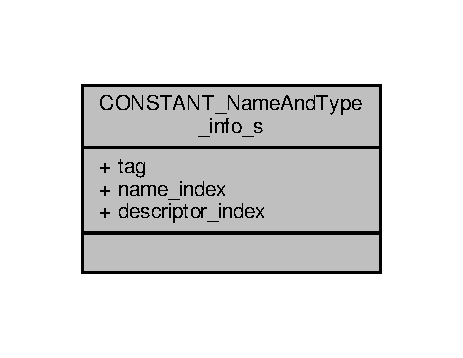
\includegraphics[width=222pt]{structCONSTANT__NameAndType__info__s__coll__graph}
\end{center}
\end{figure}
\subsection*{Public Attributes}
\begin{DoxyCompactItemize}
\item 
\hyperlink{structs_8hpp_a17947ec3f3c1f2392eabd36c1ba5fec6}{cp\+\_\+tag} \hyperlink{structCONSTANT__NameAndType__info__s_af1309f9a1be5883b8fd62f0ddb624556}{tag}
\item 
uint16\+\_\+t \hyperlink{structCONSTANT__NameAndType__info__s_af552a69c9df4e87b43cc278ff6a21e51}{name\+\_\+index}
\item 
uint16\+\_\+t \hyperlink{structCONSTANT__NameAndType__info__s_a18a7d7ce834fbc08bbf856e0528e6383}{descriptor\+\_\+index}
\end{DoxyCompactItemize}


\subsection{Member Data Documentation}
\hypertarget{structCONSTANT__NameAndType__info__s_a18a7d7ce834fbc08bbf856e0528e6383}{\index{C\+O\+N\+S\+T\+A\+N\+T\+\_\+\+Name\+And\+Type\+\_\+info\+\_\+s@{C\+O\+N\+S\+T\+A\+N\+T\+\_\+\+Name\+And\+Type\+\_\+info\+\_\+s}!descriptor\+\_\+index@{descriptor\+\_\+index}}
\index{descriptor\+\_\+index@{descriptor\+\_\+index}!C\+O\+N\+S\+T\+A\+N\+T\+\_\+\+Name\+And\+Type\+\_\+info\+\_\+s@{C\+O\+N\+S\+T\+A\+N\+T\+\_\+\+Name\+And\+Type\+\_\+info\+\_\+s}}
\subsubsection[{descriptor\+\_\+index}]{\setlength{\rightskip}{0pt plus 5cm}uint16\+\_\+t C\+O\+N\+S\+T\+A\+N\+T\+\_\+\+Name\+And\+Type\+\_\+info\+\_\+s\+::descriptor\+\_\+index}}\label{structCONSTANT__NameAndType__info__s_a18a7d7ce834fbc08bbf856e0528e6383}
\hypertarget{structCONSTANT__NameAndType__info__s_af552a69c9df4e87b43cc278ff6a21e51}{\index{C\+O\+N\+S\+T\+A\+N\+T\+\_\+\+Name\+And\+Type\+\_\+info\+\_\+s@{C\+O\+N\+S\+T\+A\+N\+T\+\_\+\+Name\+And\+Type\+\_\+info\+\_\+s}!name\+\_\+index@{name\+\_\+index}}
\index{name\+\_\+index@{name\+\_\+index}!C\+O\+N\+S\+T\+A\+N\+T\+\_\+\+Name\+And\+Type\+\_\+info\+\_\+s@{C\+O\+N\+S\+T\+A\+N\+T\+\_\+\+Name\+And\+Type\+\_\+info\+\_\+s}}
\subsubsection[{name\+\_\+index}]{\setlength{\rightskip}{0pt plus 5cm}uint16\+\_\+t C\+O\+N\+S\+T\+A\+N\+T\+\_\+\+Name\+And\+Type\+\_\+info\+\_\+s\+::name\+\_\+index}}\label{structCONSTANT__NameAndType__info__s_af552a69c9df4e87b43cc278ff6a21e51}
\hypertarget{structCONSTANT__NameAndType__info__s_af1309f9a1be5883b8fd62f0ddb624556}{\index{C\+O\+N\+S\+T\+A\+N\+T\+\_\+\+Name\+And\+Type\+\_\+info\+\_\+s@{C\+O\+N\+S\+T\+A\+N\+T\+\_\+\+Name\+And\+Type\+\_\+info\+\_\+s}!tag@{tag}}
\index{tag@{tag}!C\+O\+N\+S\+T\+A\+N\+T\+\_\+\+Name\+And\+Type\+\_\+info\+\_\+s@{C\+O\+N\+S\+T\+A\+N\+T\+\_\+\+Name\+And\+Type\+\_\+info\+\_\+s}}
\subsubsection[{tag}]{\setlength{\rightskip}{0pt plus 5cm}{\bf cp\+\_\+tag} C\+O\+N\+S\+T\+A\+N\+T\+\_\+\+Name\+And\+Type\+\_\+info\+\_\+s\+::tag}}\label{structCONSTANT__NameAndType__info__s_af1309f9a1be5883b8fd62f0ddb624556}


The documentation for this struct was generated from the following file\+:\begin{DoxyCompactItemize}
\item 
include/\hyperlink{structs_8hpp}{structs.\+hpp}\end{DoxyCompactItemize}

\hypertarget{structCONSTANT__String__info__s}{\section{C\+O\+N\+S\+T\+A\+N\+T\+\_\+\+String\+\_\+info\+\_\+s Struct Reference}
\label{structCONSTANT__String__info__s}\index{C\+O\+N\+S\+T\+A\+N\+T\+\_\+\+String\+\_\+info\+\_\+s@{C\+O\+N\+S\+T\+A\+N\+T\+\_\+\+String\+\_\+info\+\_\+s}}
}


{\ttfamily \#include $<$structs.\+hpp$>$}



Collaboration diagram for C\+O\+N\+S\+T\+A\+N\+T\+\_\+\+String\+\_\+info\+\_\+s\+:\nopagebreak
\begin{figure}[H]
\begin{center}
\leavevmode
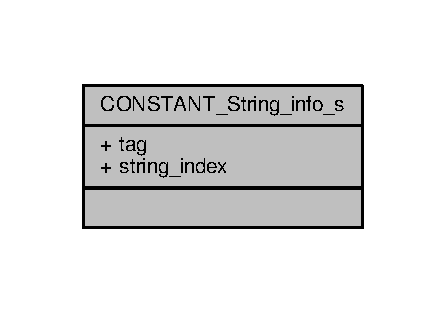
\includegraphics[width=214pt]{structCONSTANT__String__info__s__coll__graph}
\end{center}
\end{figure}
\subsection*{Public Attributes}
\begin{DoxyCompactItemize}
\item 
\hyperlink{structs_8hpp_a17947ec3f3c1f2392eabd36c1ba5fec6}{cp\+\_\+tag} \hyperlink{structCONSTANT__String__info__s_a63a92aabe2638ad427f912551c99c18a}{tag}
\item 
uint16\+\_\+t \hyperlink{structCONSTANT__String__info__s_a9fb8030b5c3bbfca53934e67991399cf}{string\+\_\+index}
\end{DoxyCompactItemize}


\subsection{Member Data Documentation}
\hypertarget{structCONSTANT__String__info__s_a9fb8030b5c3bbfca53934e67991399cf}{\index{C\+O\+N\+S\+T\+A\+N\+T\+\_\+\+String\+\_\+info\+\_\+s@{C\+O\+N\+S\+T\+A\+N\+T\+\_\+\+String\+\_\+info\+\_\+s}!string\+\_\+index@{string\+\_\+index}}
\index{string\+\_\+index@{string\+\_\+index}!C\+O\+N\+S\+T\+A\+N\+T\+\_\+\+String\+\_\+info\+\_\+s@{C\+O\+N\+S\+T\+A\+N\+T\+\_\+\+String\+\_\+info\+\_\+s}}
\subsubsection[{string\+\_\+index}]{\setlength{\rightskip}{0pt plus 5cm}uint16\+\_\+t C\+O\+N\+S\+T\+A\+N\+T\+\_\+\+String\+\_\+info\+\_\+s\+::string\+\_\+index}}\label{structCONSTANT__String__info__s_a9fb8030b5c3bbfca53934e67991399cf}
\hypertarget{structCONSTANT__String__info__s_a63a92aabe2638ad427f912551c99c18a}{\index{C\+O\+N\+S\+T\+A\+N\+T\+\_\+\+String\+\_\+info\+\_\+s@{C\+O\+N\+S\+T\+A\+N\+T\+\_\+\+String\+\_\+info\+\_\+s}!tag@{tag}}
\index{tag@{tag}!C\+O\+N\+S\+T\+A\+N\+T\+\_\+\+String\+\_\+info\+\_\+s@{C\+O\+N\+S\+T\+A\+N\+T\+\_\+\+String\+\_\+info\+\_\+s}}
\subsubsection[{tag}]{\setlength{\rightskip}{0pt plus 5cm}{\bf cp\+\_\+tag} C\+O\+N\+S\+T\+A\+N\+T\+\_\+\+String\+\_\+info\+\_\+s\+::tag}}\label{structCONSTANT__String__info__s_a63a92aabe2638ad427f912551c99c18a}


The documentation for this struct was generated from the following file\+:\begin{DoxyCompactItemize}
\item 
include/\hyperlink{structs_8hpp}{structs.\+hpp}\end{DoxyCompactItemize}

\hypertarget{structCONSTANT__Utf8__info__s}{\section{C\+O\+N\+S\+T\+A\+N\+T\+\_\+\+Utf8\+\_\+info\+\_\+s Struct Reference}
\label{structCONSTANT__Utf8__info__s}\index{C\+O\+N\+S\+T\+A\+N\+T\+\_\+\+Utf8\+\_\+info\+\_\+s@{C\+O\+N\+S\+T\+A\+N\+T\+\_\+\+Utf8\+\_\+info\+\_\+s}}
}


{\ttfamily \#include $<$structs.\+hpp$>$}



Collaboration diagram for C\+O\+N\+S\+T\+A\+N\+T\+\_\+\+Utf8\+\_\+info\+\_\+s\+:\nopagebreak
\begin{figure}[H]
\begin{center}
\leavevmode
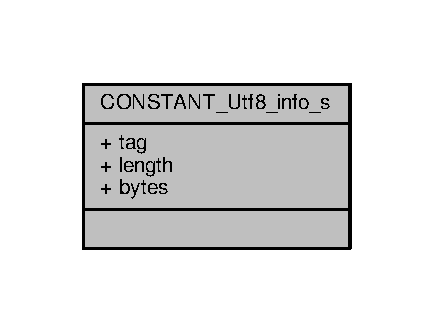
\includegraphics[width=208pt]{structCONSTANT__Utf8__info__s__coll__graph}
\end{center}
\end{figure}
\subsection*{Public Attributes}
\begin{DoxyCompactItemize}
\item 
\hyperlink{structs_8hpp_a17947ec3f3c1f2392eabd36c1ba5fec6}{cp\+\_\+tag} \hyperlink{structCONSTANT__Utf8__info__s_a7af843af8dd80fb01a548d38aa7cf649}{tag}
\item 
uint16\+\_\+t \hyperlink{structCONSTANT__Utf8__info__s_a9e45087cd112ac744db73614e4ffef05}{length}
\item 
char $\ast$ \hyperlink{structCONSTANT__Utf8__info__s_a773fbbd37e847eba505fa36f948f3bb5}{bytes}
\end{DoxyCompactItemize}


\subsection{Member Data Documentation}
\hypertarget{structCONSTANT__Utf8__info__s_a773fbbd37e847eba505fa36f948f3bb5}{\index{C\+O\+N\+S\+T\+A\+N\+T\+\_\+\+Utf8\+\_\+info\+\_\+s@{C\+O\+N\+S\+T\+A\+N\+T\+\_\+\+Utf8\+\_\+info\+\_\+s}!bytes@{bytes}}
\index{bytes@{bytes}!C\+O\+N\+S\+T\+A\+N\+T\+\_\+\+Utf8\+\_\+info\+\_\+s@{C\+O\+N\+S\+T\+A\+N\+T\+\_\+\+Utf8\+\_\+info\+\_\+s}}
\subsubsection[{bytes}]{\setlength{\rightskip}{0pt plus 5cm}char$\ast$ C\+O\+N\+S\+T\+A\+N\+T\+\_\+\+Utf8\+\_\+info\+\_\+s\+::bytes}}\label{structCONSTANT__Utf8__info__s_a773fbbd37e847eba505fa36f948f3bb5}
\hypertarget{structCONSTANT__Utf8__info__s_a9e45087cd112ac744db73614e4ffef05}{\index{C\+O\+N\+S\+T\+A\+N\+T\+\_\+\+Utf8\+\_\+info\+\_\+s@{C\+O\+N\+S\+T\+A\+N\+T\+\_\+\+Utf8\+\_\+info\+\_\+s}!length@{length}}
\index{length@{length}!C\+O\+N\+S\+T\+A\+N\+T\+\_\+\+Utf8\+\_\+info\+\_\+s@{C\+O\+N\+S\+T\+A\+N\+T\+\_\+\+Utf8\+\_\+info\+\_\+s}}
\subsubsection[{length}]{\setlength{\rightskip}{0pt plus 5cm}uint16\+\_\+t C\+O\+N\+S\+T\+A\+N\+T\+\_\+\+Utf8\+\_\+info\+\_\+s\+::length}}\label{structCONSTANT__Utf8__info__s_a9e45087cd112ac744db73614e4ffef05}
\hypertarget{structCONSTANT__Utf8__info__s_a7af843af8dd80fb01a548d38aa7cf649}{\index{C\+O\+N\+S\+T\+A\+N\+T\+\_\+\+Utf8\+\_\+info\+\_\+s@{C\+O\+N\+S\+T\+A\+N\+T\+\_\+\+Utf8\+\_\+info\+\_\+s}!tag@{tag}}
\index{tag@{tag}!C\+O\+N\+S\+T\+A\+N\+T\+\_\+\+Utf8\+\_\+info\+\_\+s@{C\+O\+N\+S\+T\+A\+N\+T\+\_\+\+Utf8\+\_\+info\+\_\+s}}
\subsubsection[{tag}]{\setlength{\rightskip}{0pt plus 5cm}{\bf cp\+\_\+tag} C\+O\+N\+S\+T\+A\+N\+T\+\_\+\+Utf8\+\_\+info\+\_\+s\+::tag}}\label{structCONSTANT__Utf8__info__s_a7af843af8dd80fb01a548d38aa7cf649}


The documentation for this struct was generated from the following file\+:\begin{DoxyCompactItemize}
\item 
include/\hyperlink{structs_8hpp}{structs.\+hpp}\end{DoxyCompactItemize}

\hypertarget{structConstantValue__attribute__s}{\section{Constant\+Value\+\_\+attribute\+\_\+s Struct Reference}
\label{structConstantValue__attribute__s}\index{Constant\+Value\+\_\+attribute\+\_\+s@{Constant\+Value\+\_\+attribute\+\_\+s}}
}


{\ttfamily \#include $<$attributes.\+hpp$>$}



Collaboration diagram for Constant\+Value\+\_\+attribute\+\_\+s\+:\nopagebreak
\begin{figure}[H]
\begin{center}
\leavevmode
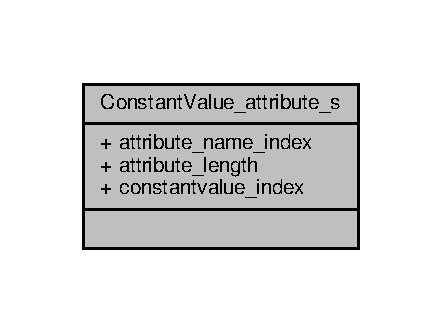
\includegraphics[width=212pt]{structConstantValue__attribute__s__coll__graph}
\end{center}
\end{figure}
\subsection*{Public Attributes}
\begin{DoxyCompactItemize}
\item 
uint16\+\_\+t \hyperlink{structConstantValue__attribute__s_a8811aed2a17e628c96b323d7e7c22edd}{attribute\+\_\+name\+\_\+index}
\item 
uint32\+\_\+t \hyperlink{structConstantValue__attribute__s_a0de6a32434624a71a93ca95870a2e727}{attribute\+\_\+length}
\item 
uint16\+\_\+t \hyperlink{structConstantValue__attribute__s_a50669a8c13452c0bc3283d182223a131}{constantvalue\+\_\+index}
\end{DoxyCompactItemize}


\subsection{Member Data Documentation}
\hypertarget{structConstantValue__attribute__s_a0de6a32434624a71a93ca95870a2e727}{\index{Constant\+Value\+\_\+attribute\+\_\+s@{Constant\+Value\+\_\+attribute\+\_\+s}!attribute\+\_\+length@{attribute\+\_\+length}}
\index{attribute\+\_\+length@{attribute\+\_\+length}!Constant\+Value\+\_\+attribute\+\_\+s@{Constant\+Value\+\_\+attribute\+\_\+s}}
\subsubsection[{attribute\+\_\+length}]{\setlength{\rightskip}{0pt plus 5cm}uint32\+\_\+t Constant\+Value\+\_\+attribute\+\_\+s\+::attribute\+\_\+length}}\label{structConstantValue__attribute__s_a0de6a32434624a71a93ca95870a2e727}
\hypertarget{structConstantValue__attribute__s_a8811aed2a17e628c96b323d7e7c22edd}{\index{Constant\+Value\+\_\+attribute\+\_\+s@{Constant\+Value\+\_\+attribute\+\_\+s}!attribute\+\_\+name\+\_\+index@{attribute\+\_\+name\+\_\+index}}
\index{attribute\+\_\+name\+\_\+index@{attribute\+\_\+name\+\_\+index}!Constant\+Value\+\_\+attribute\+\_\+s@{Constant\+Value\+\_\+attribute\+\_\+s}}
\subsubsection[{attribute\+\_\+name\+\_\+index}]{\setlength{\rightskip}{0pt plus 5cm}uint16\+\_\+t Constant\+Value\+\_\+attribute\+\_\+s\+::attribute\+\_\+name\+\_\+index}}\label{structConstantValue__attribute__s_a8811aed2a17e628c96b323d7e7c22edd}
\hypertarget{structConstantValue__attribute__s_a50669a8c13452c0bc3283d182223a131}{\index{Constant\+Value\+\_\+attribute\+\_\+s@{Constant\+Value\+\_\+attribute\+\_\+s}!constantvalue\+\_\+index@{constantvalue\+\_\+index}}
\index{constantvalue\+\_\+index@{constantvalue\+\_\+index}!Constant\+Value\+\_\+attribute\+\_\+s@{Constant\+Value\+\_\+attribute\+\_\+s}}
\subsubsection[{constantvalue\+\_\+index}]{\setlength{\rightskip}{0pt plus 5cm}uint16\+\_\+t Constant\+Value\+\_\+attribute\+\_\+s\+::constantvalue\+\_\+index}}\label{structConstantValue__attribute__s_a50669a8c13452c0bc3283d182223a131}


The documentation for this struct was generated from the following file\+:\begin{DoxyCompactItemize}
\item 
include/\hyperlink{attributes_8hpp}{attributes.\+hpp}\end{DoxyCompactItemize}

\hypertarget{structcp__info__s}{\section{cp\+\_\+info\+\_\+s Struct Reference}
\label{structcp__info__s}\index{cp\+\_\+info\+\_\+s@{cp\+\_\+info\+\_\+s}}
}


{\ttfamily \#include $<$structs.\+hpp$>$}



Collaboration diagram for cp\+\_\+info\+\_\+s\+:\nopagebreak
\begin{figure}[H]
\begin{center}
\leavevmode
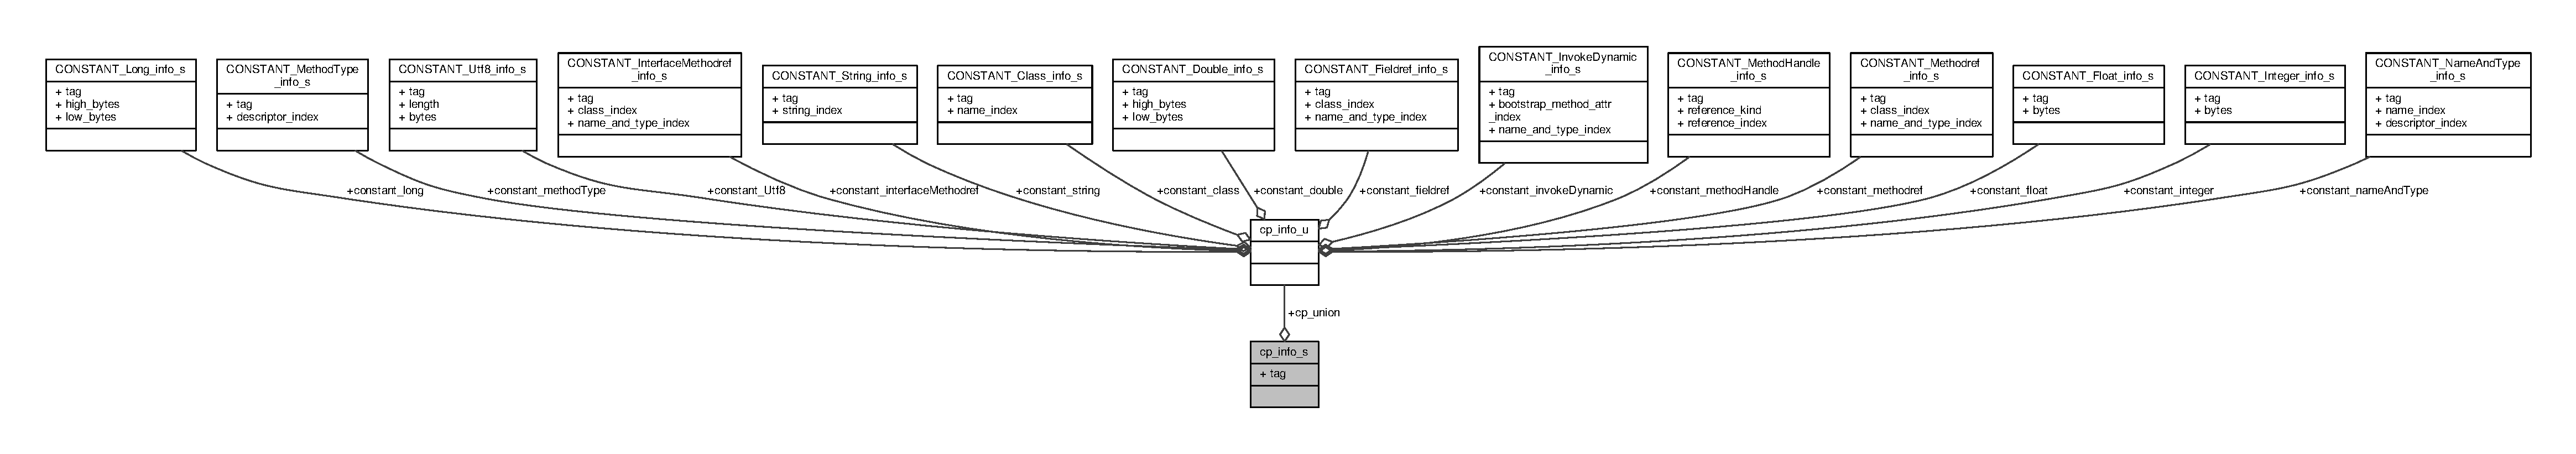
\includegraphics[width=350pt]{structcp__info__s__coll__graph}
\end{center}
\end{figure}
\subsection*{Public Attributes}
\begin{DoxyCompactItemize}
\item 
\hyperlink{structs_8hpp_a17947ec3f3c1f2392eabd36c1ba5fec6}{cp\+\_\+tag} \hyperlink{structcp__info__s_a6b3587f422119dbdd9fa778d383c787a}{tag}
\item 
\hyperlink{structs_8hpp_af9cb1bd49e931147183cfb411f105f09}{cp\+Info\+\_\+u} \hyperlink{structcp__info__s_a099688c74e2156e544e235b636f68f8a}{cp\+\_\+union}
\end{DoxyCompactItemize}


\subsection{Member Data Documentation}
\hypertarget{structcp__info__s_a099688c74e2156e544e235b636f68f8a}{\index{cp\+\_\+info\+\_\+s@{cp\+\_\+info\+\_\+s}!cp\+\_\+union@{cp\+\_\+union}}
\index{cp\+\_\+union@{cp\+\_\+union}!cp\+\_\+info\+\_\+s@{cp\+\_\+info\+\_\+s}}
\subsubsection[{cp\+\_\+union}]{\setlength{\rightskip}{0pt plus 5cm}{\bf cp\+Info\+\_\+u} cp\+\_\+info\+\_\+s\+::cp\+\_\+union}}\label{structcp__info__s_a099688c74e2156e544e235b636f68f8a}
\hypertarget{structcp__info__s_a6b3587f422119dbdd9fa778d383c787a}{\index{cp\+\_\+info\+\_\+s@{cp\+\_\+info\+\_\+s}!tag@{tag}}
\index{tag@{tag}!cp\+\_\+info\+\_\+s@{cp\+\_\+info\+\_\+s}}
\subsubsection[{tag}]{\setlength{\rightskip}{0pt plus 5cm}{\bf cp\+\_\+tag} cp\+\_\+info\+\_\+s\+::tag}}\label{structcp__info__s_a6b3587f422119dbdd9fa778d383c787a}


The documentation for this struct was generated from the following file\+:\begin{DoxyCompactItemize}
\item 
include/\hyperlink{structs_8hpp}{structs.\+hpp}\end{DoxyCompactItemize}

\hypertarget{unioncp__info__u}{\section{cp\+\_\+info\+\_\+u Union Reference}
\label{unioncp__info__u}\index{cp\+\_\+info\+\_\+u@{cp\+\_\+info\+\_\+u}}
}


{\ttfamily \#include $<$structs.\+hpp$>$}



Collaboration diagram for cp\+\_\+info\+\_\+u\+:\nopagebreak
\begin{figure}[H]
\begin{center}
\leavevmode
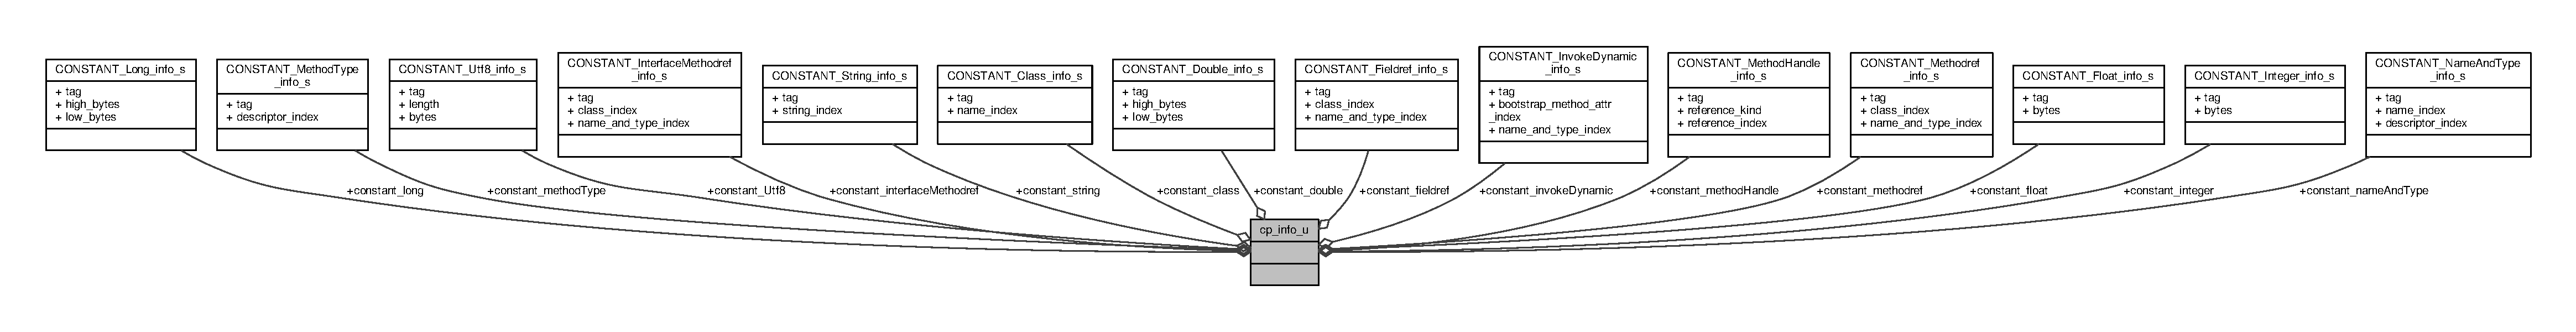
\includegraphics[width=350pt]{unioncp__info__u__coll__graph}
\end{center}
\end{figure}
\subsection*{Public Attributes}
\begin{DoxyCompactItemize}
\item 
\hyperlink{structs_8hpp_afce1973b88cef62148562ed37fbbdfec}{C\+O\+N\+S\+T\+A\+N\+T\+\_\+\+Class\+\_\+info} \hyperlink{unioncp__info__u_aa80a68381f1daf2ccf6ac2ee5ce9b602}{constant\+\_\+class}
\item 
\hyperlink{structs_8hpp_a5b79c4752ea4a4e4880f374239e23104}{C\+O\+N\+S\+T\+A\+N\+T\+\_\+\+Fieldref\+\_\+info} \hyperlink{unioncp__info__u_a18be3ffc26ebc8887f507dd9e6cb756c}{constant\+\_\+fieldref}
\item 
\hyperlink{structs_8hpp_a11dfb795f76c8ae500e5652924ba7289}{C\+O\+N\+S\+T\+A\+N\+T\+\_\+\+Methodref\+\_\+info} \hyperlink{unioncp__info__u_a1b1c3cd5733f2a29bb0e2814b67f168d}{constant\+\_\+methodref}
\item 
\hyperlink{structs_8hpp_a5d8a806561391610f7092cae2e9fbdca}{C\+O\+N\+S\+T\+A\+N\+T\+\_\+\+Interface\+Methodref\+\_\+info} \hyperlink{unioncp__info__u_a15e8972d564add1f129d469b54efb8b6}{constant\+\_\+interface\+Methodref}
\item 
\hyperlink{structs_8hpp_a98fe2dcb4f443548bca1e1ba4750551d}{C\+O\+N\+S\+T\+A\+N\+T\+\_\+\+String\+\_\+info} \hyperlink{unioncp__info__u_acd87a20b30ed9024d98239c3cd14b0f9}{constant\+\_\+string}
\item 
\hyperlink{structs_8hpp_a787b138703e5fbe6f5899de13d7dcb63}{C\+O\+N\+S\+T\+A\+N\+T\+\_\+\+Integer\+\_\+info} \hyperlink{unioncp__info__u_aef67ff0a71fe8f3a8a6f276c0e177c9c}{constant\+\_\+integer}
\item 
\hyperlink{structs_8hpp_af49965517a6dbed7ccaeeae09beb251a}{C\+O\+N\+S\+T\+A\+N\+T\+\_\+\+Float\+\_\+info} \hyperlink{unioncp__info__u_a14b943c747f6aa0fe799739608439fd9}{constant\+\_\+float}
\item 
\hyperlink{structs_8hpp_a0664b73f95a5ba329c2f70bf22c70cb8}{C\+O\+N\+S\+T\+A\+N\+T\+\_\+\+Long\+\_\+info} \hyperlink{unioncp__info__u_aac563b3b1991dd783a7dcf8734cc7b68}{constant\+\_\+long}
\item 
\hyperlink{structs_8hpp_a2c42e32589ba5c1bb09cabcadcb0f96c}{C\+O\+N\+S\+T\+A\+N\+T\+\_\+\+Double\+\_\+info} \hyperlink{unioncp__info__u_a564a2f753c2487b102b95c993596a103}{constant\+\_\+double}
\item 
\hyperlink{structs_8hpp_ab09f323602f4043c3f40d009f3f3b84c}{C\+O\+N\+S\+T\+A\+N\+T\+\_\+\+Name\+And\+Type\+\_\+info} \hyperlink{unioncp__info__u_a238fa508b12d3cba9a428ac2b8183eff}{constant\+\_\+name\+And\+Type}
\item 
\hyperlink{structs_8hpp_a2c99a23a5dec8fe5e86498bb0fc1a18d}{C\+O\+N\+S\+T\+A\+N\+T\+\_\+\+Utf8\+\_\+info} \hyperlink{unioncp__info__u_a0a674b77186bea6da5c1f1311ba1b594}{constant\+\_\+\+Utf8}
\item 
\hyperlink{structs_8hpp_a863e6b2ab8603c43c0072809b41adf0c}{C\+O\+N\+S\+T\+A\+N\+T\+\_\+\+Method\+Handle\+\_\+info} \hyperlink{unioncp__info__u_afc136c55fd02b88bb21a5aae24514025}{constant\+\_\+method\+Handle}
\item 
\hyperlink{structs_8hpp_a8885b4c01b5d7217e80864ad1019696a}{C\+O\+N\+S\+T\+A\+N\+T\+\_\+\+Method\+Type\+\_\+info} \hyperlink{unioncp__info__u_ae7a8f3a0c5a809fe6342411d8908e615}{constant\+\_\+method\+Type}
\item 
\hyperlink{structs_8hpp_a2537ef8ea7dec99c077fd6a3c3c619ff}{C\+O\+N\+S\+T\+A\+N\+T\+\_\+\+Invoke\+Dynamic\+\_\+info} \hyperlink{unioncp__info__u_ac0f54cc7ccab5abb2eb1a89410cf1936}{constant\+\_\+invoke\+Dynamic}
\end{DoxyCompactItemize}


\subsection{Member Data Documentation}
\hypertarget{unioncp__info__u_aa80a68381f1daf2ccf6ac2ee5ce9b602}{\index{cp\+\_\+info\+\_\+u@{cp\+\_\+info\+\_\+u}!constant\+\_\+class@{constant\+\_\+class}}
\index{constant\+\_\+class@{constant\+\_\+class}!cp\+\_\+info\+\_\+u@{cp\+\_\+info\+\_\+u}}
\subsubsection[{constant\+\_\+class}]{\setlength{\rightskip}{0pt plus 5cm}{\bf C\+O\+N\+S\+T\+A\+N\+T\+\_\+\+Class\+\_\+info} cp\+\_\+info\+\_\+u\+::constant\+\_\+class}}\label{unioncp__info__u_aa80a68381f1daf2ccf6ac2ee5ce9b602}
\hypertarget{unioncp__info__u_a564a2f753c2487b102b95c993596a103}{\index{cp\+\_\+info\+\_\+u@{cp\+\_\+info\+\_\+u}!constant\+\_\+double@{constant\+\_\+double}}
\index{constant\+\_\+double@{constant\+\_\+double}!cp\+\_\+info\+\_\+u@{cp\+\_\+info\+\_\+u}}
\subsubsection[{constant\+\_\+double}]{\setlength{\rightskip}{0pt plus 5cm}{\bf C\+O\+N\+S\+T\+A\+N\+T\+\_\+\+Double\+\_\+info} cp\+\_\+info\+\_\+u\+::constant\+\_\+double}}\label{unioncp__info__u_a564a2f753c2487b102b95c993596a103}
\hypertarget{unioncp__info__u_a18be3ffc26ebc8887f507dd9e6cb756c}{\index{cp\+\_\+info\+\_\+u@{cp\+\_\+info\+\_\+u}!constant\+\_\+fieldref@{constant\+\_\+fieldref}}
\index{constant\+\_\+fieldref@{constant\+\_\+fieldref}!cp\+\_\+info\+\_\+u@{cp\+\_\+info\+\_\+u}}
\subsubsection[{constant\+\_\+fieldref}]{\setlength{\rightskip}{0pt plus 5cm}{\bf C\+O\+N\+S\+T\+A\+N\+T\+\_\+\+Fieldref\+\_\+info} cp\+\_\+info\+\_\+u\+::constant\+\_\+fieldref}}\label{unioncp__info__u_a18be3ffc26ebc8887f507dd9e6cb756c}
\hypertarget{unioncp__info__u_a14b943c747f6aa0fe799739608439fd9}{\index{cp\+\_\+info\+\_\+u@{cp\+\_\+info\+\_\+u}!constant\+\_\+float@{constant\+\_\+float}}
\index{constant\+\_\+float@{constant\+\_\+float}!cp\+\_\+info\+\_\+u@{cp\+\_\+info\+\_\+u}}
\subsubsection[{constant\+\_\+float}]{\setlength{\rightskip}{0pt plus 5cm}{\bf C\+O\+N\+S\+T\+A\+N\+T\+\_\+\+Float\+\_\+info} cp\+\_\+info\+\_\+u\+::constant\+\_\+float}}\label{unioncp__info__u_a14b943c747f6aa0fe799739608439fd9}
\hypertarget{unioncp__info__u_aef67ff0a71fe8f3a8a6f276c0e177c9c}{\index{cp\+\_\+info\+\_\+u@{cp\+\_\+info\+\_\+u}!constant\+\_\+integer@{constant\+\_\+integer}}
\index{constant\+\_\+integer@{constant\+\_\+integer}!cp\+\_\+info\+\_\+u@{cp\+\_\+info\+\_\+u}}
\subsubsection[{constant\+\_\+integer}]{\setlength{\rightskip}{0pt plus 5cm}{\bf C\+O\+N\+S\+T\+A\+N\+T\+\_\+\+Integer\+\_\+info} cp\+\_\+info\+\_\+u\+::constant\+\_\+integer}}\label{unioncp__info__u_aef67ff0a71fe8f3a8a6f276c0e177c9c}
\hypertarget{unioncp__info__u_a15e8972d564add1f129d469b54efb8b6}{\index{cp\+\_\+info\+\_\+u@{cp\+\_\+info\+\_\+u}!constant\+\_\+interface\+Methodref@{constant\+\_\+interface\+Methodref}}
\index{constant\+\_\+interface\+Methodref@{constant\+\_\+interface\+Methodref}!cp\+\_\+info\+\_\+u@{cp\+\_\+info\+\_\+u}}
\subsubsection[{constant\+\_\+interface\+Methodref}]{\setlength{\rightskip}{0pt plus 5cm}{\bf C\+O\+N\+S\+T\+A\+N\+T\+\_\+\+Interface\+Methodref\+\_\+info} cp\+\_\+info\+\_\+u\+::constant\+\_\+interface\+Methodref}}\label{unioncp__info__u_a15e8972d564add1f129d469b54efb8b6}
\hypertarget{unioncp__info__u_ac0f54cc7ccab5abb2eb1a89410cf1936}{\index{cp\+\_\+info\+\_\+u@{cp\+\_\+info\+\_\+u}!constant\+\_\+invoke\+Dynamic@{constant\+\_\+invoke\+Dynamic}}
\index{constant\+\_\+invoke\+Dynamic@{constant\+\_\+invoke\+Dynamic}!cp\+\_\+info\+\_\+u@{cp\+\_\+info\+\_\+u}}
\subsubsection[{constant\+\_\+invoke\+Dynamic}]{\setlength{\rightskip}{0pt plus 5cm}{\bf C\+O\+N\+S\+T\+A\+N\+T\+\_\+\+Invoke\+Dynamic\+\_\+info} cp\+\_\+info\+\_\+u\+::constant\+\_\+invoke\+Dynamic}}\label{unioncp__info__u_ac0f54cc7ccab5abb2eb1a89410cf1936}
\hypertarget{unioncp__info__u_aac563b3b1991dd783a7dcf8734cc7b68}{\index{cp\+\_\+info\+\_\+u@{cp\+\_\+info\+\_\+u}!constant\+\_\+long@{constant\+\_\+long}}
\index{constant\+\_\+long@{constant\+\_\+long}!cp\+\_\+info\+\_\+u@{cp\+\_\+info\+\_\+u}}
\subsubsection[{constant\+\_\+long}]{\setlength{\rightskip}{0pt plus 5cm}{\bf C\+O\+N\+S\+T\+A\+N\+T\+\_\+\+Long\+\_\+info} cp\+\_\+info\+\_\+u\+::constant\+\_\+long}}\label{unioncp__info__u_aac563b3b1991dd783a7dcf8734cc7b68}
\hypertarget{unioncp__info__u_afc136c55fd02b88bb21a5aae24514025}{\index{cp\+\_\+info\+\_\+u@{cp\+\_\+info\+\_\+u}!constant\+\_\+method\+Handle@{constant\+\_\+method\+Handle}}
\index{constant\+\_\+method\+Handle@{constant\+\_\+method\+Handle}!cp\+\_\+info\+\_\+u@{cp\+\_\+info\+\_\+u}}
\subsubsection[{constant\+\_\+method\+Handle}]{\setlength{\rightskip}{0pt plus 5cm}{\bf C\+O\+N\+S\+T\+A\+N\+T\+\_\+\+Method\+Handle\+\_\+info} cp\+\_\+info\+\_\+u\+::constant\+\_\+method\+Handle}}\label{unioncp__info__u_afc136c55fd02b88bb21a5aae24514025}
\hypertarget{unioncp__info__u_a1b1c3cd5733f2a29bb0e2814b67f168d}{\index{cp\+\_\+info\+\_\+u@{cp\+\_\+info\+\_\+u}!constant\+\_\+methodref@{constant\+\_\+methodref}}
\index{constant\+\_\+methodref@{constant\+\_\+methodref}!cp\+\_\+info\+\_\+u@{cp\+\_\+info\+\_\+u}}
\subsubsection[{constant\+\_\+methodref}]{\setlength{\rightskip}{0pt plus 5cm}{\bf C\+O\+N\+S\+T\+A\+N\+T\+\_\+\+Methodref\+\_\+info} cp\+\_\+info\+\_\+u\+::constant\+\_\+methodref}}\label{unioncp__info__u_a1b1c3cd5733f2a29bb0e2814b67f168d}
\hypertarget{unioncp__info__u_ae7a8f3a0c5a809fe6342411d8908e615}{\index{cp\+\_\+info\+\_\+u@{cp\+\_\+info\+\_\+u}!constant\+\_\+method\+Type@{constant\+\_\+method\+Type}}
\index{constant\+\_\+method\+Type@{constant\+\_\+method\+Type}!cp\+\_\+info\+\_\+u@{cp\+\_\+info\+\_\+u}}
\subsubsection[{constant\+\_\+method\+Type}]{\setlength{\rightskip}{0pt plus 5cm}{\bf C\+O\+N\+S\+T\+A\+N\+T\+\_\+\+Method\+Type\+\_\+info} cp\+\_\+info\+\_\+u\+::constant\+\_\+method\+Type}}\label{unioncp__info__u_ae7a8f3a0c5a809fe6342411d8908e615}
\hypertarget{unioncp__info__u_a238fa508b12d3cba9a428ac2b8183eff}{\index{cp\+\_\+info\+\_\+u@{cp\+\_\+info\+\_\+u}!constant\+\_\+name\+And\+Type@{constant\+\_\+name\+And\+Type}}
\index{constant\+\_\+name\+And\+Type@{constant\+\_\+name\+And\+Type}!cp\+\_\+info\+\_\+u@{cp\+\_\+info\+\_\+u}}
\subsubsection[{constant\+\_\+name\+And\+Type}]{\setlength{\rightskip}{0pt plus 5cm}{\bf C\+O\+N\+S\+T\+A\+N\+T\+\_\+\+Name\+And\+Type\+\_\+info} cp\+\_\+info\+\_\+u\+::constant\+\_\+name\+And\+Type}}\label{unioncp__info__u_a238fa508b12d3cba9a428ac2b8183eff}
\hypertarget{unioncp__info__u_acd87a20b30ed9024d98239c3cd14b0f9}{\index{cp\+\_\+info\+\_\+u@{cp\+\_\+info\+\_\+u}!constant\+\_\+string@{constant\+\_\+string}}
\index{constant\+\_\+string@{constant\+\_\+string}!cp\+\_\+info\+\_\+u@{cp\+\_\+info\+\_\+u}}
\subsubsection[{constant\+\_\+string}]{\setlength{\rightskip}{0pt plus 5cm}{\bf C\+O\+N\+S\+T\+A\+N\+T\+\_\+\+String\+\_\+info} cp\+\_\+info\+\_\+u\+::constant\+\_\+string}}\label{unioncp__info__u_acd87a20b30ed9024d98239c3cd14b0f9}
\hypertarget{unioncp__info__u_a0a674b77186bea6da5c1f1311ba1b594}{\index{cp\+\_\+info\+\_\+u@{cp\+\_\+info\+\_\+u}!constant\+\_\+\+Utf8@{constant\+\_\+\+Utf8}}
\index{constant\+\_\+\+Utf8@{constant\+\_\+\+Utf8}!cp\+\_\+info\+\_\+u@{cp\+\_\+info\+\_\+u}}
\subsubsection[{constant\+\_\+\+Utf8}]{\setlength{\rightskip}{0pt plus 5cm}{\bf C\+O\+N\+S\+T\+A\+N\+T\+\_\+\+Utf8\+\_\+info} cp\+\_\+info\+\_\+u\+::constant\+\_\+\+Utf8}}\label{unioncp__info__u_a0a674b77186bea6da5c1f1311ba1b594}


The documentation for this union was generated from the following file\+:\begin{DoxyCompactItemize}
\item 
include/\hyperlink{structs_8hpp}{structs.\+hpp}\end{DoxyCompactItemize}

\hypertarget{structDeprecated__attribute__s}{\section{Deprecated\+\_\+attribute\+\_\+s Struct Reference}
\label{structDeprecated__attribute__s}\index{Deprecated\+\_\+attribute\+\_\+s@{Deprecated\+\_\+attribute\+\_\+s}}
}


{\ttfamily \#include $<$attributes.\+hpp$>$}



Collaboration diagram for Deprecated\+\_\+attribute\+\_\+s\+:\nopagebreak
\begin{figure}[H]
\begin{center}
\leavevmode
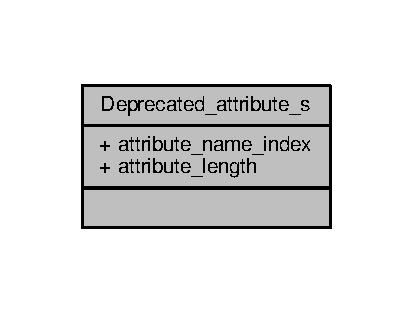
\includegraphics[width=198pt]{structDeprecated__attribute__s__coll__graph}
\end{center}
\end{figure}
\subsection*{Public Attributes}
\begin{DoxyCompactItemize}
\item 
uint16\+\_\+t \hyperlink{structDeprecated__attribute__s_ad8fd16bc95d09719922224c303248ca9}{attribute\+\_\+name\+\_\+index}
\item 
uint32\+\_\+t \hyperlink{structDeprecated__attribute__s_a5c1b473858ed1435598d5ce11ae8a0c3}{attribute\+\_\+length}
\end{DoxyCompactItemize}


\subsection{Member Data Documentation}
\hypertarget{structDeprecated__attribute__s_a5c1b473858ed1435598d5ce11ae8a0c3}{\index{Deprecated\+\_\+attribute\+\_\+s@{Deprecated\+\_\+attribute\+\_\+s}!attribute\+\_\+length@{attribute\+\_\+length}}
\index{attribute\+\_\+length@{attribute\+\_\+length}!Deprecated\+\_\+attribute\+\_\+s@{Deprecated\+\_\+attribute\+\_\+s}}
\subsubsection[{attribute\+\_\+length}]{\setlength{\rightskip}{0pt plus 5cm}uint32\+\_\+t Deprecated\+\_\+attribute\+\_\+s\+::attribute\+\_\+length}}\label{structDeprecated__attribute__s_a5c1b473858ed1435598d5ce11ae8a0c3}
\hypertarget{structDeprecated__attribute__s_ad8fd16bc95d09719922224c303248ca9}{\index{Deprecated\+\_\+attribute\+\_\+s@{Deprecated\+\_\+attribute\+\_\+s}!attribute\+\_\+name\+\_\+index@{attribute\+\_\+name\+\_\+index}}
\index{attribute\+\_\+name\+\_\+index@{attribute\+\_\+name\+\_\+index}!Deprecated\+\_\+attribute\+\_\+s@{Deprecated\+\_\+attribute\+\_\+s}}
\subsubsection[{attribute\+\_\+name\+\_\+index}]{\setlength{\rightskip}{0pt plus 5cm}uint16\+\_\+t Deprecated\+\_\+attribute\+\_\+s\+::attribute\+\_\+name\+\_\+index}}\label{structDeprecated__attribute__s_ad8fd16bc95d09719922224c303248ca9}


The documentation for this struct was generated from the following file\+:\begin{DoxyCompactItemize}
\item 
include/\hyperlink{attributes_8hpp}{attributes.\+hpp}\end{DoxyCompactItemize}

\hypertarget{structEnclosingMethod__attribute__s}{\section{Enclosing\+Method\+\_\+attribute\+\_\+s Struct Reference}
\label{structEnclosingMethod__attribute__s}\index{Enclosing\+Method\+\_\+attribute\+\_\+s@{Enclosing\+Method\+\_\+attribute\+\_\+s}}
}


{\ttfamily \#include $<$attributes.\+hpp$>$}



Collaboration diagram for Enclosing\+Method\+\_\+attribute\+\_\+s\+:\nopagebreak
\begin{figure}[H]
\begin{center}
\leavevmode
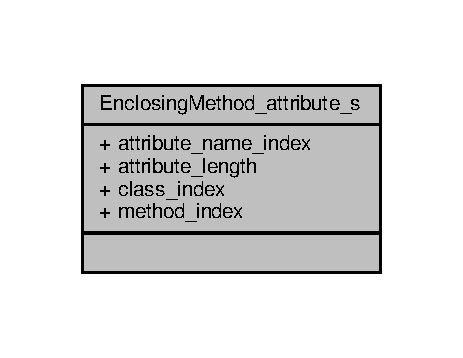
\includegraphics[width=222pt]{structEnclosingMethod__attribute__s__coll__graph}
\end{center}
\end{figure}
\subsection*{Public Attributes}
\begin{DoxyCompactItemize}
\item 
uint16\+\_\+t \hyperlink{structEnclosingMethod__attribute__s_ad2b896b9d74117aadabfcc0a451f0df4}{attribute\+\_\+name\+\_\+index}
\item 
uint32\+\_\+t \hyperlink{structEnclosingMethod__attribute__s_a47d67cf5da95073e23f63b07819726ac}{attribute\+\_\+length}
\item 
uint16\+\_\+t \hyperlink{structEnclosingMethod__attribute__s_a4f0350de4c8297324b3d4fa1afd5e5f8}{class\+\_\+index}
\item 
uint16\+\_\+t \hyperlink{structEnclosingMethod__attribute__s_ab6428de4b25c84e1ef61d3c806932823}{method\+\_\+index}
\end{DoxyCompactItemize}


\subsection{Member Data Documentation}
\hypertarget{structEnclosingMethod__attribute__s_a47d67cf5da95073e23f63b07819726ac}{\index{Enclosing\+Method\+\_\+attribute\+\_\+s@{Enclosing\+Method\+\_\+attribute\+\_\+s}!attribute\+\_\+length@{attribute\+\_\+length}}
\index{attribute\+\_\+length@{attribute\+\_\+length}!Enclosing\+Method\+\_\+attribute\+\_\+s@{Enclosing\+Method\+\_\+attribute\+\_\+s}}
\subsubsection[{attribute\+\_\+length}]{\setlength{\rightskip}{0pt plus 5cm}uint32\+\_\+t Enclosing\+Method\+\_\+attribute\+\_\+s\+::attribute\+\_\+length}}\label{structEnclosingMethod__attribute__s_a47d67cf5da95073e23f63b07819726ac}
\hypertarget{structEnclosingMethod__attribute__s_ad2b896b9d74117aadabfcc0a451f0df4}{\index{Enclosing\+Method\+\_\+attribute\+\_\+s@{Enclosing\+Method\+\_\+attribute\+\_\+s}!attribute\+\_\+name\+\_\+index@{attribute\+\_\+name\+\_\+index}}
\index{attribute\+\_\+name\+\_\+index@{attribute\+\_\+name\+\_\+index}!Enclosing\+Method\+\_\+attribute\+\_\+s@{Enclosing\+Method\+\_\+attribute\+\_\+s}}
\subsubsection[{attribute\+\_\+name\+\_\+index}]{\setlength{\rightskip}{0pt plus 5cm}uint16\+\_\+t Enclosing\+Method\+\_\+attribute\+\_\+s\+::attribute\+\_\+name\+\_\+index}}\label{structEnclosingMethod__attribute__s_ad2b896b9d74117aadabfcc0a451f0df4}
\hypertarget{structEnclosingMethod__attribute__s_a4f0350de4c8297324b3d4fa1afd5e5f8}{\index{Enclosing\+Method\+\_\+attribute\+\_\+s@{Enclosing\+Method\+\_\+attribute\+\_\+s}!class\+\_\+index@{class\+\_\+index}}
\index{class\+\_\+index@{class\+\_\+index}!Enclosing\+Method\+\_\+attribute\+\_\+s@{Enclosing\+Method\+\_\+attribute\+\_\+s}}
\subsubsection[{class\+\_\+index}]{\setlength{\rightskip}{0pt plus 5cm}uint16\+\_\+t Enclosing\+Method\+\_\+attribute\+\_\+s\+::class\+\_\+index}}\label{structEnclosingMethod__attribute__s_a4f0350de4c8297324b3d4fa1afd5e5f8}
\hypertarget{structEnclosingMethod__attribute__s_ab6428de4b25c84e1ef61d3c806932823}{\index{Enclosing\+Method\+\_\+attribute\+\_\+s@{Enclosing\+Method\+\_\+attribute\+\_\+s}!method\+\_\+index@{method\+\_\+index}}
\index{method\+\_\+index@{method\+\_\+index}!Enclosing\+Method\+\_\+attribute\+\_\+s@{Enclosing\+Method\+\_\+attribute\+\_\+s}}
\subsubsection[{method\+\_\+index}]{\setlength{\rightskip}{0pt plus 5cm}uint16\+\_\+t Enclosing\+Method\+\_\+attribute\+\_\+s\+::method\+\_\+index}}\label{structEnclosingMethod__attribute__s_ab6428de4b25c84e1ef61d3c806932823}


The documentation for this struct was generated from the following file\+:\begin{DoxyCompactItemize}
\item 
include/\hyperlink{attributes_8hpp}{attributes.\+hpp}\end{DoxyCompactItemize}

\hypertarget{structexception__table__info__s}{\section{exception\+\_\+table\+\_\+info\+\_\+s Struct Reference}
\label{structexception__table__info__s}\index{exception\+\_\+table\+\_\+info\+\_\+s@{exception\+\_\+table\+\_\+info\+\_\+s}}
}


{\ttfamily \#include $<$attributes.\+hpp$>$}



Collaboration diagram for exception\+\_\+table\+\_\+info\+\_\+s\+:\nopagebreak
\begin{figure}[H]
\begin{center}
\leavevmode
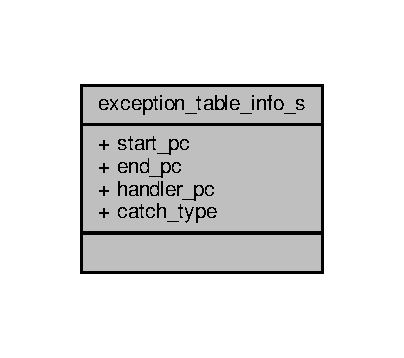
\includegraphics[width=194pt]{structexception__table__info__s__coll__graph}
\end{center}
\end{figure}
\subsection*{Public Attributes}
\begin{DoxyCompactItemize}
\item 
uint16\+\_\+t \hyperlink{structexception__table__info__s_ae92c43a2d7c711e34fda9bc778e7019c}{start\+\_\+pc}
\item 
uint16\+\_\+t \hyperlink{structexception__table__info__s_ab7f40660c6dfb31d0d33443f8631a86b}{end\+\_\+pc}
\item 
uint16\+\_\+t \hyperlink{structexception__table__info__s_afce7361ca9bc44352ab13a94890d7644}{handler\+\_\+pc}
\item 
uint16\+\_\+t \hyperlink{structexception__table__info__s_a797170f960fb0a1797a69bca7a1567d0}{catch\+\_\+type}
\end{DoxyCompactItemize}


\subsection{Member Data Documentation}
\hypertarget{structexception__table__info__s_a797170f960fb0a1797a69bca7a1567d0}{\index{exception\+\_\+table\+\_\+info\+\_\+s@{exception\+\_\+table\+\_\+info\+\_\+s}!catch\+\_\+type@{catch\+\_\+type}}
\index{catch\+\_\+type@{catch\+\_\+type}!exception\+\_\+table\+\_\+info\+\_\+s@{exception\+\_\+table\+\_\+info\+\_\+s}}
\subsubsection[{catch\+\_\+type}]{\setlength{\rightskip}{0pt plus 5cm}uint16\+\_\+t exception\+\_\+table\+\_\+info\+\_\+s\+::catch\+\_\+type}}\label{structexception__table__info__s_a797170f960fb0a1797a69bca7a1567d0}
\hypertarget{structexception__table__info__s_ab7f40660c6dfb31d0d33443f8631a86b}{\index{exception\+\_\+table\+\_\+info\+\_\+s@{exception\+\_\+table\+\_\+info\+\_\+s}!end\+\_\+pc@{end\+\_\+pc}}
\index{end\+\_\+pc@{end\+\_\+pc}!exception\+\_\+table\+\_\+info\+\_\+s@{exception\+\_\+table\+\_\+info\+\_\+s}}
\subsubsection[{end\+\_\+pc}]{\setlength{\rightskip}{0pt plus 5cm}uint16\+\_\+t exception\+\_\+table\+\_\+info\+\_\+s\+::end\+\_\+pc}}\label{structexception__table__info__s_ab7f40660c6dfb31d0d33443f8631a86b}
\hypertarget{structexception__table__info__s_afce7361ca9bc44352ab13a94890d7644}{\index{exception\+\_\+table\+\_\+info\+\_\+s@{exception\+\_\+table\+\_\+info\+\_\+s}!handler\+\_\+pc@{handler\+\_\+pc}}
\index{handler\+\_\+pc@{handler\+\_\+pc}!exception\+\_\+table\+\_\+info\+\_\+s@{exception\+\_\+table\+\_\+info\+\_\+s}}
\subsubsection[{handler\+\_\+pc}]{\setlength{\rightskip}{0pt plus 5cm}uint16\+\_\+t exception\+\_\+table\+\_\+info\+\_\+s\+::handler\+\_\+pc}}\label{structexception__table__info__s_afce7361ca9bc44352ab13a94890d7644}
\hypertarget{structexception__table__info__s_ae92c43a2d7c711e34fda9bc778e7019c}{\index{exception\+\_\+table\+\_\+info\+\_\+s@{exception\+\_\+table\+\_\+info\+\_\+s}!start\+\_\+pc@{start\+\_\+pc}}
\index{start\+\_\+pc@{start\+\_\+pc}!exception\+\_\+table\+\_\+info\+\_\+s@{exception\+\_\+table\+\_\+info\+\_\+s}}
\subsubsection[{start\+\_\+pc}]{\setlength{\rightskip}{0pt plus 5cm}uint16\+\_\+t exception\+\_\+table\+\_\+info\+\_\+s\+::start\+\_\+pc}}\label{structexception__table__info__s_ae92c43a2d7c711e34fda9bc778e7019c}


The documentation for this struct was generated from the following file\+:\begin{DoxyCompactItemize}
\item 
include/\hyperlink{attributes_8hpp}{attributes.\+hpp}\end{DoxyCompactItemize}

\hypertarget{structfield__info__s}{\section{field\+\_\+info\+\_\+s Struct Reference}
\label{structfield__info__s}\index{field\+\_\+info\+\_\+s@{field\+\_\+info\+\_\+s}}
}


{\ttfamily \#include $<$structs.\+hpp$>$}



Collaboration diagram for field\+\_\+info\+\_\+s\+:\nopagebreak
\begin{figure}[H]
\begin{center}
\leavevmode
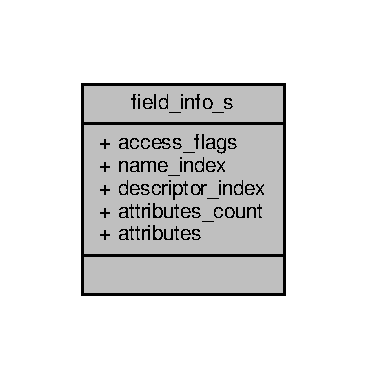
\includegraphics[width=176pt]{structfield__info__s__coll__graph}
\end{center}
\end{figure}
\subsection*{Public Attributes}
\begin{DoxyCompactItemize}
\item 
uint16\+\_\+t \hyperlink{structfield__info__s_a51cb65a206e19f1ef167f808fd0dd34a}{access\+\_\+flags}
\item 
uint16\+\_\+t \hyperlink{structfield__info__s_ae6ad0227620df9c8733e10a29b320957}{name\+\_\+index}
\item 
uint16\+\_\+t \hyperlink{structfield__info__s_acf1b97dc1bf435aa19f77bc6131a7055}{descriptor\+\_\+index}
\item 
uint16\+\_\+t \hyperlink{structfield__info__s_ada4b62d8b973680b456f6c397db8cb11}{attributes\+\_\+count}
\item 
std\+::vector$<$ \hyperlink{attributes_8hpp_a7af51299ff517acce960ac87c9db9899}{attribute\+\_\+info} $>$ \hyperlink{structfield__info__s_a77c8bf8802039e9dbf1b3b69a55ace29}{attributes}
\end{DoxyCompactItemize}


\subsection{Member Data Documentation}
\hypertarget{structfield__info__s_a51cb65a206e19f1ef167f808fd0dd34a}{\index{field\+\_\+info\+\_\+s@{field\+\_\+info\+\_\+s}!access\+\_\+flags@{access\+\_\+flags}}
\index{access\+\_\+flags@{access\+\_\+flags}!field\+\_\+info\+\_\+s@{field\+\_\+info\+\_\+s}}
\subsubsection[{access\+\_\+flags}]{\setlength{\rightskip}{0pt plus 5cm}uint16\+\_\+t field\+\_\+info\+\_\+s\+::access\+\_\+flags}}\label{structfield__info__s_a51cb65a206e19f1ef167f808fd0dd34a}
\hypertarget{structfield__info__s_a77c8bf8802039e9dbf1b3b69a55ace29}{\index{field\+\_\+info\+\_\+s@{field\+\_\+info\+\_\+s}!attributes@{attributes}}
\index{attributes@{attributes}!field\+\_\+info\+\_\+s@{field\+\_\+info\+\_\+s}}
\subsubsection[{attributes}]{\setlength{\rightskip}{0pt plus 5cm}std\+::vector$<${\bf attribute\+\_\+info}$>$ field\+\_\+info\+\_\+s\+::attributes}}\label{structfield__info__s_a77c8bf8802039e9dbf1b3b69a55ace29}
\hypertarget{structfield__info__s_ada4b62d8b973680b456f6c397db8cb11}{\index{field\+\_\+info\+\_\+s@{field\+\_\+info\+\_\+s}!attributes\+\_\+count@{attributes\+\_\+count}}
\index{attributes\+\_\+count@{attributes\+\_\+count}!field\+\_\+info\+\_\+s@{field\+\_\+info\+\_\+s}}
\subsubsection[{attributes\+\_\+count}]{\setlength{\rightskip}{0pt plus 5cm}uint16\+\_\+t field\+\_\+info\+\_\+s\+::attributes\+\_\+count}}\label{structfield__info__s_ada4b62d8b973680b456f6c397db8cb11}
\hypertarget{structfield__info__s_acf1b97dc1bf435aa19f77bc6131a7055}{\index{field\+\_\+info\+\_\+s@{field\+\_\+info\+\_\+s}!descriptor\+\_\+index@{descriptor\+\_\+index}}
\index{descriptor\+\_\+index@{descriptor\+\_\+index}!field\+\_\+info\+\_\+s@{field\+\_\+info\+\_\+s}}
\subsubsection[{descriptor\+\_\+index}]{\setlength{\rightskip}{0pt plus 5cm}uint16\+\_\+t field\+\_\+info\+\_\+s\+::descriptor\+\_\+index}}\label{structfield__info__s_acf1b97dc1bf435aa19f77bc6131a7055}
\hypertarget{structfield__info__s_ae6ad0227620df9c8733e10a29b320957}{\index{field\+\_\+info\+\_\+s@{field\+\_\+info\+\_\+s}!name\+\_\+index@{name\+\_\+index}}
\index{name\+\_\+index@{name\+\_\+index}!field\+\_\+info\+\_\+s@{field\+\_\+info\+\_\+s}}
\subsubsection[{name\+\_\+index}]{\setlength{\rightskip}{0pt plus 5cm}uint16\+\_\+t field\+\_\+info\+\_\+s\+::name\+\_\+index}}\label{structfield__info__s_ae6ad0227620df9c8733e10a29b320957}


The documentation for this struct was generated from the following file\+:\begin{DoxyCompactItemize}
\item 
include/\hyperlink{structs_8hpp}{structs.\+hpp}\end{DoxyCompactItemize}

\hypertarget{structfield__value__s}{\section{field\+\_\+value\+\_\+s Struct Reference}
\label{structfield__value__s}\index{field\+\_\+value\+\_\+s@{field\+\_\+value\+\_\+s}}
}


{\ttfamily \#include $<$heap.\+hpp$>$}



Collaboration diagram for field\+\_\+value\+\_\+s\+:\nopagebreak
\begin{figure}[H]
\begin{center}
\leavevmode
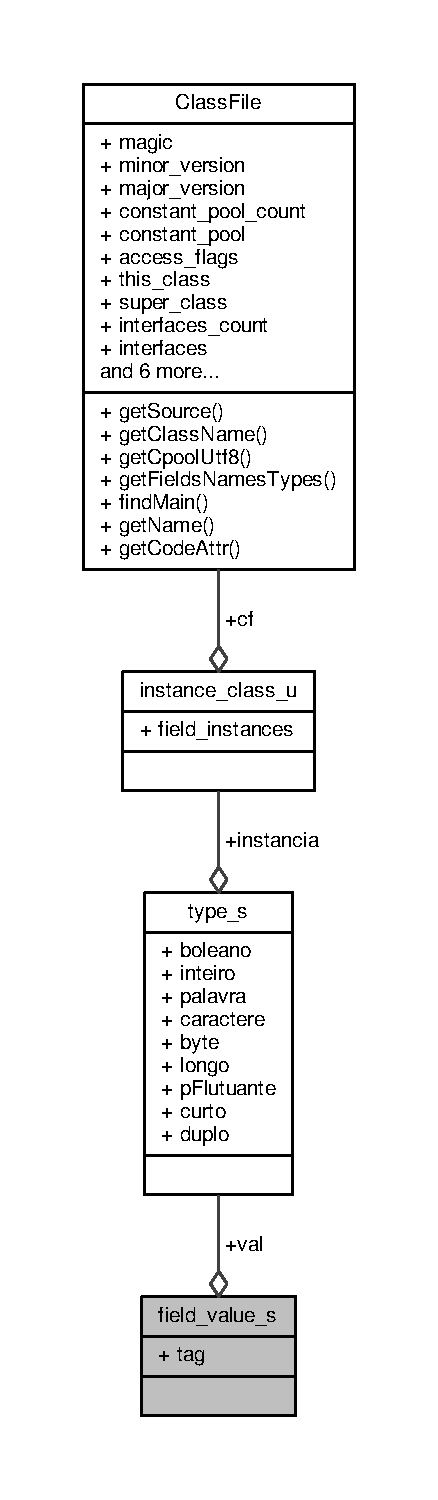
\includegraphics[height=550pt]{structfield__value__s__coll__graph}
\end{center}
\end{figure}
\subsection*{Public Attributes}
\begin{DoxyCompactItemize}
\item 
uint8\+\_\+t \hyperlink{structfield__value__s_a4fe2c4d897f539e3b0f3d50ecc5083c1}{tag}
\item 
\hyperlink{heap_8hpp_ae5c0f9a3fc75861baaa7475c345f119d}{field\+\_\+type} \hyperlink{structfield__value__s_ac2dfcee3f37fc6387bbf5b7a9a5eeb6b}{val}
\end{DoxyCompactItemize}


\subsection{Member Data Documentation}
\hypertarget{structfield__value__s_a4fe2c4d897f539e3b0f3d50ecc5083c1}{\index{field\+\_\+value\+\_\+s@{field\+\_\+value\+\_\+s}!tag@{tag}}
\index{tag@{tag}!field\+\_\+value\+\_\+s@{field\+\_\+value\+\_\+s}}
\subsubsection[{tag}]{\setlength{\rightskip}{0pt plus 5cm}uint8\+\_\+t field\+\_\+value\+\_\+s\+::tag}}\label{structfield__value__s_a4fe2c4d897f539e3b0f3d50ecc5083c1}
\hypertarget{structfield__value__s_ac2dfcee3f37fc6387bbf5b7a9a5eeb6b}{\index{field\+\_\+value\+\_\+s@{field\+\_\+value\+\_\+s}!val@{val}}
\index{val@{val}!field\+\_\+value\+\_\+s@{field\+\_\+value\+\_\+s}}
\subsubsection[{val}]{\setlength{\rightskip}{0pt plus 5cm}{\bf field\+\_\+type} field\+\_\+value\+\_\+s\+::val}}\label{structfield__value__s_ac2dfcee3f37fc6387bbf5b7a9a5eeb6b}


The documentation for this struct was generated from the following file\+:\begin{DoxyCompactItemize}
\item 
include/\hyperlink{heap_8hpp}{heap.\+hpp}\end{DoxyCompactItemize}

\hypertarget{classFrame}{\section{Frame Class Reference}
\label{classFrame}\index{Frame@{Frame}}
}


{\ttfamily \#include $<$frame.\+hpp$>$}



Collaboration diagram for Frame\+:\nopagebreak
\begin{figure}[H]
\begin{center}
\leavevmode
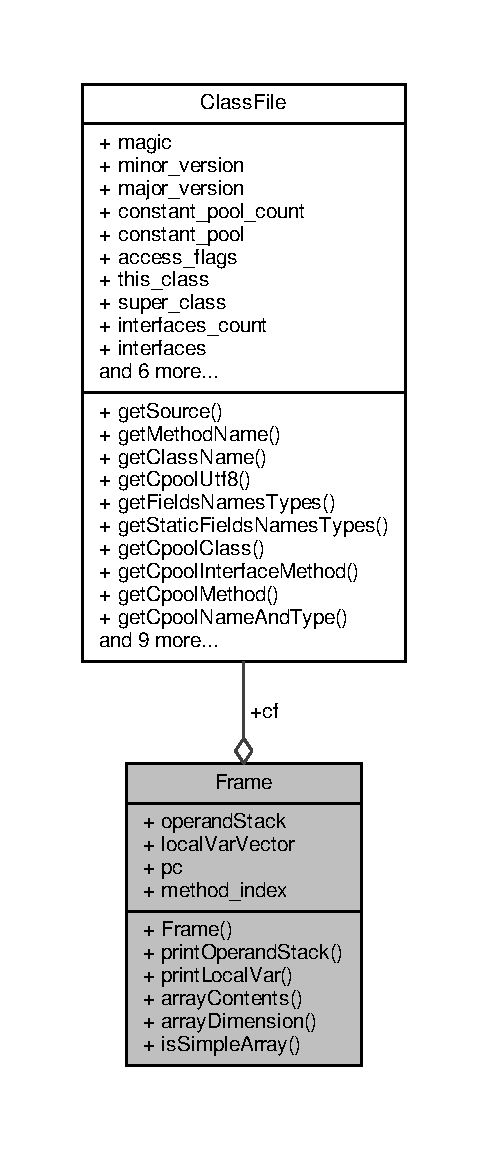
\includegraphics[width=234pt]{classFrame__coll__graph}
\end{center}
\end{figure}
\subsection*{Public Member Functions}
\begin{DoxyCompactItemize}
\item 
\hyperlink{classFrame_a0a710d74c28a542687e64715300cb8fb}{Frame} (int \hyperlink{classFrame_a9a7eb96be80ac389517368b48f88e1f5}{method\+\_\+index}, \hyperlink{classClassFile}{Class\+File} $\ast$\hyperlink{classFrame_a1adaa34d477660f1e9d45904576eacf2}{cf})
\item 
void \hyperlink{classFrame_a58199d48ff5d3b2c86aea6f79a8ccf10}{print\+Operand\+Stack} ()
\item 
void \hyperlink{classFrame_ab34a9033d268d94f205721b63101b047}{print\+Local\+Var} ()
\end{DoxyCompactItemize}
\subsection*{Public Attributes}
\begin{DoxyCompactItemize}
\item 
std\+::vector$<$ \hyperlink{classLocal__var}{Local\+\_\+var} $>$ \hyperlink{classFrame_ad8d3859aa247f9ea26ed70734dd93141}{operand\+Stack}
\begin{DoxyCompactList}\small\item\em Pilha de operandos. A pilha de operandos começa vazia. Ela é populada ao longo da execução das instruções. \end{DoxyCompactList}\item 
std\+::vector$<$ \hyperlink{classLocal__var}{Local\+\_\+var} $>$ \hyperlink{classFrame_ab3b3b8b51af39a6c4b76bc99bffd8808}{local\+Var\+Vector}
\begin{DoxyCompactList}\small\item\em Vetor de variáveis locais. \end{DoxyCompactList}\item 
uint64\+\_\+t \hyperlink{classFrame_a65edf2210e6653b9acbdc58240040104}{pc}
\begin{DoxyCompactList}\small\item\em Código atual sendo executado. \end{DoxyCompactList}\item 
\hyperlink{classClassFile}{Class\+File} $\ast$ \hyperlink{classFrame_a1adaa34d477660f1e9d45904576eacf2}{cf}
\begin{DoxyCompactList}\small\item\em referencia pra constant pool \end{DoxyCompactList}\item 
int \hyperlink{classFrame_a9a7eb96be80ac389517368b48f88e1f5}{method\+\_\+index}
\begin{DoxyCompactList}\small\item\em esta será a variável que identifica qual método da cf estamos rodando \end{DoxyCompactList}\end{DoxyCompactItemize}


\subsection{Constructor \& Destructor Documentation}
\hypertarget{classFrame_a0a710d74c28a542687e64715300cb8fb}{\index{Frame@{Frame}!Frame@{Frame}}
\index{Frame@{Frame}!Frame@{Frame}}
\subsubsection[{Frame}]{\setlength{\rightskip}{0pt plus 5cm}Frame\+::\+Frame (
\begin{DoxyParamCaption}
\item[{int}]{method\+\_\+index, }
\item[{{\bf Class\+File} $\ast$}]{cf}
\end{DoxyParamCaption}
)}}\label{classFrame_a0a710d74c28a542687e64715300cb8fb}


\subsection{Member Function Documentation}
\hypertarget{classFrame_ab34a9033d268d94f205721b63101b047}{\index{Frame@{Frame}!print\+Local\+Var@{print\+Local\+Var}}
\index{print\+Local\+Var@{print\+Local\+Var}!Frame@{Frame}}
\subsubsection[{print\+Local\+Var}]{\setlength{\rightskip}{0pt plus 5cm}void Frame\+::print\+Local\+Var (
\begin{DoxyParamCaption}
{}
\end{DoxyParamCaption}
)}}\label{classFrame_ab34a9033d268d94f205721b63101b047}
\hypertarget{classFrame_a58199d48ff5d3b2c86aea6f79a8ccf10}{\index{Frame@{Frame}!print\+Operand\+Stack@{print\+Operand\+Stack}}
\index{print\+Operand\+Stack@{print\+Operand\+Stack}!Frame@{Frame}}
\subsubsection[{print\+Operand\+Stack}]{\setlength{\rightskip}{0pt plus 5cm}void Frame\+::print\+Operand\+Stack (
\begin{DoxyParamCaption}
{}
\end{DoxyParamCaption}
)}}\label{classFrame_a58199d48ff5d3b2c86aea6f79a8ccf10}


\subsection{Member Data Documentation}
\hypertarget{classFrame_a1adaa34d477660f1e9d45904576eacf2}{\index{Frame@{Frame}!cf@{cf}}
\index{cf@{cf}!Frame@{Frame}}
\subsubsection[{cf}]{\setlength{\rightskip}{0pt plus 5cm}$\ast$ Frame\+::cf}}\label{classFrame_a1adaa34d477660f1e9d45904576eacf2}


referencia pra constant pool 

\hypertarget{classFrame_ab3b3b8b51af39a6c4b76bc99bffd8808}{\index{Frame@{Frame}!local\+Var\+Vector@{local\+Var\+Vector}}
\index{local\+Var\+Vector@{local\+Var\+Vector}!Frame@{Frame}}
\subsubsection[{local\+Var\+Vector}]{\setlength{\rightskip}{0pt plus 5cm}Frame\+::local\+Var\+Vector}}\label{classFrame_ab3b3b8b51af39a6c4b76bc99bffd8808}


Vetor de variáveis locais. 

\hypertarget{classFrame_a9a7eb96be80ac389517368b48f88e1f5}{\index{Frame@{Frame}!method\+\_\+index@{method\+\_\+index}}
\index{method\+\_\+index@{method\+\_\+index}!Frame@{Frame}}
\subsubsection[{method\+\_\+index}]{\setlength{\rightskip}{0pt plus 5cm}Frame\+::method\+\_\+index}}\label{classFrame_a9a7eb96be80ac389517368b48f88e1f5}


esta será a variável que identifica qual método da cf estamos rodando 

\hypertarget{classFrame_ad8d3859aa247f9ea26ed70734dd93141}{\index{Frame@{Frame}!operand\+Stack@{operand\+Stack}}
\index{operand\+Stack@{operand\+Stack}!Frame@{Frame}}
\subsubsection[{operand\+Stack}]{\setlength{\rightskip}{0pt plus 5cm}Frame\+::operand\+Stack}}\label{classFrame_ad8d3859aa247f9ea26ed70734dd93141}


Pilha de operandos. A pilha de operandos começa vazia. Ela é populada ao longo da execução das instruções. 

\hypertarget{classFrame_a65edf2210e6653b9acbdc58240040104}{\index{Frame@{Frame}!pc@{pc}}
\index{pc@{pc}!Frame@{Frame}}
\subsubsection[{pc}]{\setlength{\rightskip}{0pt plus 5cm}Frame\+::pc}}\label{classFrame_a65edf2210e6653b9acbdc58240040104}


Código atual sendo executado. 



The documentation for this class was generated from the following files\+:\begin{DoxyCompactItemize}
\item 
include/\hyperlink{frame_8hpp}{frame.\+hpp}\item 
src/\hyperlink{frame_8cpp}{frame.\+cpp}\end{DoxyCompactItemize}

\hypertarget{structInnerClasses__attribute__s}{\section{Inner\+Classes\+\_\+attribute\+\_\+s Struct Reference}
\label{structInnerClasses__attribute__s}\index{Inner\+Classes\+\_\+attribute\+\_\+s@{Inner\+Classes\+\_\+attribute\+\_\+s}}
}


{\ttfamily \#include $<$attributes.\+hpp$>$}



Collaboration diagram for Inner\+Classes\+\_\+attribute\+\_\+s\+:\nopagebreak
\begin{figure}[H]
\begin{center}
\leavevmode
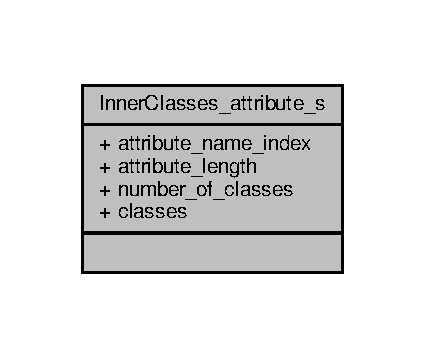
\includegraphics[width=204pt]{structInnerClasses__attribute__s__coll__graph}
\end{center}
\end{figure}
\subsection*{Public Attributes}
\begin{DoxyCompactItemize}
\item 
uint16\+\_\+t \hyperlink{structInnerClasses__attribute__s_a8ea7a6459f4a7ae27d23fa13d15b058c}{attribute\+\_\+name\+\_\+index}
\item 
uint32\+\_\+t \hyperlink{structInnerClasses__attribute__s_ab142de1a85a18b4fa3f49b77668fcd4f}{attribute\+\_\+length}
\item 
uint16\+\_\+t \hyperlink{structInnerClasses__attribute__s_ad5b6fc395dfe3380ec6a16df0cc618a4}{number\+\_\+of\+\_\+classes}
\item 
std\+::vector$<$ \hyperlink{classclasses__info}{classes\+\_\+info} $>$ $\ast$ \hyperlink{structInnerClasses__attribute__s_a3461afb1424fa780c0ac8053ead725f7}{classes}
\end{DoxyCompactItemize}


\subsection{Member Data Documentation}
\hypertarget{structInnerClasses__attribute__s_ab142de1a85a18b4fa3f49b77668fcd4f}{\index{Inner\+Classes\+\_\+attribute\+\_\+s@{Inner\+Classes\+\_\+attribute\+\_\+s}!attribute\+\_\+length@{attribute\+\_\+length}}
\index{attribute\+\_\+length@{attribute\+\_\+length}!Inner\+Classes\+\_\+attribute\+\_\+s@{Inner\+Classes\+\_\+attribute\+\_\+s}}
\subsubsection[{attribute\+\_\+length}]{\setlength{\rightskip}{0pt plus 5cm}uint32\+\_\+t Inner\+Classes\+\_\+attribute\+\_\+s\+::attribute\+\_\+length}}\label{structInnerClasses__attribute__s_ab142de1a85a18b4fa3f49b77668fcd4f}
\hypertarget{structInnerClasses__attribute__s_a8ea7a6459f4a7ae27d23fa13d15b058c}{\index{Inner\+Classes\+\_\+attribute\+\_\+s@{Inner\+Classes\+\_\+attribute\+\_\+s}!attribute\+\_\+name\+\_\+index@{attribute\+\_\+name\+\_\+index}}
\index{attribute\+\_\+name\+\_\+index@{attribute\+\_\+name\+\_\+index}!Inner\+Classes\+\_\+attribute\+\_\+s@{Inner\+Classes\+\_\+attribute\+\_\+s}}
\subsubsection[{attribute\+\_\+name\+\_\+index}]{\setlength{\rightskip}{0pt plus 5cm}uint16\+\_\+t Inner\+Classes\+\_\+attribute\+\_\+s\+::attribute\+\_\+name\+\_\+index}}\label{structInnerClasses__attribute__s_a8ea7a6459f4a7ae27d23fa13d15b058c}
\hypertarget{structInnerClasses__attribute__s_a3461afb1424fa780c0ac8053ead725f7}{\index{Inner\+Classes\+\_\+attribute\+\_\+s@{Inner\+Classes\+\_\+attribute\+\_\+s}!classes@{classes}}
\index{classes@{classes}!Inner\+Classes\+\_\+attribute\+\_\+s@{Inner\+Classes\+\_\+attribute\+\_\+s}}
\subsubsection[{classes}]{\setlength{\rightskip}{0pt plus 5cm}std\+::vector$<${\bf classes\+\_\+info}$>$$\ast$ Inner\+Classes\+\_\+attribute\+\_\+s\+::classes}}\label{structInnerClasses__attribute__s_a3461afb1424fa780c0ac8053ead725f7}
\hypertarget{structInnerClasses__attribute__s_ad5b6fc395dfe3380ec6a16df0cc618a4}{\index{Inner\+Classes\+\_\+attribute\+\_\+s@{Inner\+Classes\+\_\+attribute\+\_\+s}!number\+\_\+of\+\_\+classes@{number\+\_\+of\+\_\+classes}}
\index{number\+\_\+of\+\_\+classes@{number\+\_\+of\+\_\+classes}!Inner\+Classes\+\_\+attribute\+\_\+s@{Inner\+Classes\+\_\+attribute\+\_\+s}}
\subsubsection[{number\+\_\+of\+\_\+classes}]{\setlength{\rightskip}{0pt plus 5cm}uint16\+\_\+t Inner\+Classes\+\_\+attribute\+\_\+s\+::number\+\_\+of\+\_\+classes}}\label{structInnerClasses__attribute__s_ad5b6fc395dfe3380ec6a16df0cc618a4}


The documentation for this struct was generated from the following file\+:\begin{DoxyCompactItemize}
\item 
include/\hyperlink{attributes_8hpp}{attributes.\+hpp}\end{DoxyCompactItemize}

\hypertarget{structinstance__class__u}{\section{instance\+\_\+class\+\_\+u Struct Reference}
\label{structinstance__class__u}\index{instance\+\_\+class\+\_\+u@{instance\+\_\+class\+\_\+u}}
}


{\ttfamily \#include $<$heap.\+hpp$>$}



Collaboration diagram for instance\+\_\+class\+\_\+u\+:\nopagebreak
\begin{figure}[H]
\begin{center}
\leavevmode
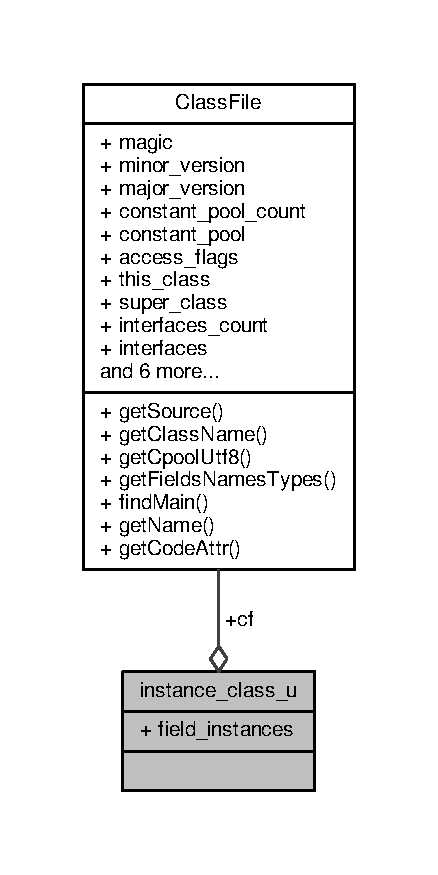
\includegraphics[width=210pt]{structinstance__class__u__coll__graph}
\end{center}
\end{figure}
\subsection*{Public Attributes}
\begin{DoxyCompactItemize}
\item 
\hyperlink{classClassFile}{Class\+File} $\ast$ \hyperlink{structinstance__class__u_a0ff637ba668f3c4a4d144c3de64eb85b}{cf}
\item 
std\+::map$<$ std\+::string, \\*
\hyperlink{heap_8hpp_a62578fb07ad4db0a96588554c6ed60b2}{field\+\_\+value} $>$ \hyperlink{structinstance__class__u_af190ac0f8c491ac92da5c237cb7dfc26}{field\+\_\+instances}
\end{DoxyCompactItemize}


\subsection{Member Data Documentation}
\hypertarget{structinstance__class__u_a0ff637ba668f3c4a4d144c3de64eb85b}{\index{instance\+\_\+class\+\_\+u@{instance\+\_\+class\+\_\+u}!cf@{cf}}
\index{cf@{cf}!instance\+\_\+class\+\_\+u@{instance\+\_\+class\+\_\+u}}
\subsubsection[{cf}]{\setlength{\rightskip}{0pt plus 5cm}{\bf Class\+File}$\ast$ instance\+\_\+class\+\_\+u\+::cf}}\label{structinstance__class__u_a0ff637ba668f3c4a4d144c3de64eb85b}
\hypertarget{structinstance__class__u_af190ac0f8c491ac92da5c237cb7dfc26}{\index{instance\+\_\+class\+\_\+u@{instance\+\_\+class\+\_\+u}!field\+\_\+instances@{field\+\_\+instances}}
\index{field\+\_\+instances@{field\+\_\+instances}!instance\+\_\+class\+\_\+u@{instance\+\_\+class\+\_\+u}}
\subsubsection[{field\+\_\+instances}]{\setlength{\rightskip}{0pt plus 5cm}std\+::map$<$std\+::string, {\bf field\+\_\+value}$>$ instance\+\_\+class\+\_\+u\+::field\+\_\+instances}}\label{structinstance__class__u_af190ac0f8c491ac92da5c237cb7dfc26}


The documentation for this struct was generated from the following file\+:\begin{DoxyCompactItemize}
\item 
include/\hyperlink{heap_8hpp}{heap.\+hpp}\end{DoxyCompactItemize}

\hypertarget{classInstructionTranslator}{\section{Instruction\+Translator Class Reference}
\label{classInstructionTranslator}\index{Instruction\+Translator@{Instruction\+Translator}}
}


{\ttfamily \#include $<$op\+\_\+instrucs.\+hpp$>$}



Collaboration diagram for Instruction\+Translator\+:\nopagebreak
\begin{figure}[H]
\begin{center}
\leavevmode
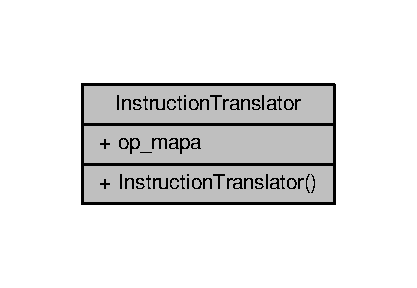
\includegraphics[width=200pt]{classInstructionTranslator__coll__graph}
\end{center}
\end{figure}
\subsection*{Public Member Functions}
\begin{DoxyCompactItemize}
\item 
\hyperlink{classInstructionTranslator_a3b5155de7dc2b808c89c486c0a6834f0}{Instruction\+Translator} ()
\end{DoxyCompactItemize}
\subsection*{Public Attributes}
\begin{DoxyCompactItemize}
\item 
std\+::map$<$ uint8\+\_\+t, std\+::string $>$ \hyperlink{classInstructionTranslator_aec4af4be8b3106a70938e03e2ff6a658}{op\+\_\+mapa}
\end{DoxyCompactItemize}


\subsection{Constructor \& Destructor Documentation}
\hypertarget{classInstructionTranslator_a3b5155de7dc2b808c89c486c0a6834f0}{\index{Instruction\+Translator@{Instruction\+Translator}!Instruction\+Translator@{Instruction\+Translator}}
\index{Instruction\+Translator@{Instruction\+Translator}!Instruction\+Translator@{Instruction\+Translator}}
\subsubsection[{Instruction\+Translator}]{\setlength{\rightskip}{0pt plus 5cm}Instruction\+Translator\+::\+Instruction\+Translator (
\begin{DoxyParamCaption}
{}
\end{DoxyParamCaption}
)}}\label{classInstructionTranslator_a3b5155de7dc2b808c89c486c0a6834f0}


\subsection{Member Data Documentation}
\hypertarget{classInstructionTranslator_aec4af4be8b3106a70938e03e2ff6a658}{\index{Instruction\+Translator@{Instruction\+Translator}!op\+\_\+mapa@{op\+\_\+mapa}}
\index{op\+\_\+mapa@{op\+\_\+mapa}!Instruction\+Translator@{Instruction\+Translator}}
\subsubsection[{op\+\_\+mapa}]{\setlength{\rightskip}{0pt plus 5cm}std\+::map$<$uint8\+\_\+t, std\+::string$>$ Instruction\+Translator\+::op\+\_\+mapa}}\label{classInstructionTranslator_aec4af4be8b3106a70938e03e2ff6a658}


The documentation for this class was generated from the following files\+:\begin{DoxyCompactItemize}
\item 
include/\hyperlink{op__instrucs_8hpp}{op\+\_\+instrucs.\+hpp}\item 
src/\hyperlink{op__instrucs_8cpp}{op\+\_\+instrucs.\+cpp}\end{DoxyCompactItemize}

\hypertarget{classInterpretador}{\section{Interpretador Class Reference}
\label{classInterpretador}\index{Interpretador@{Interpretador}}
}


{\ttfamily \#include $<$interpretador.\+hpp$>$}



Collaboration diagram for Interpretador\+:\nopagebreak
\begin{figure}[H]
\begin{center}
\leavevmode
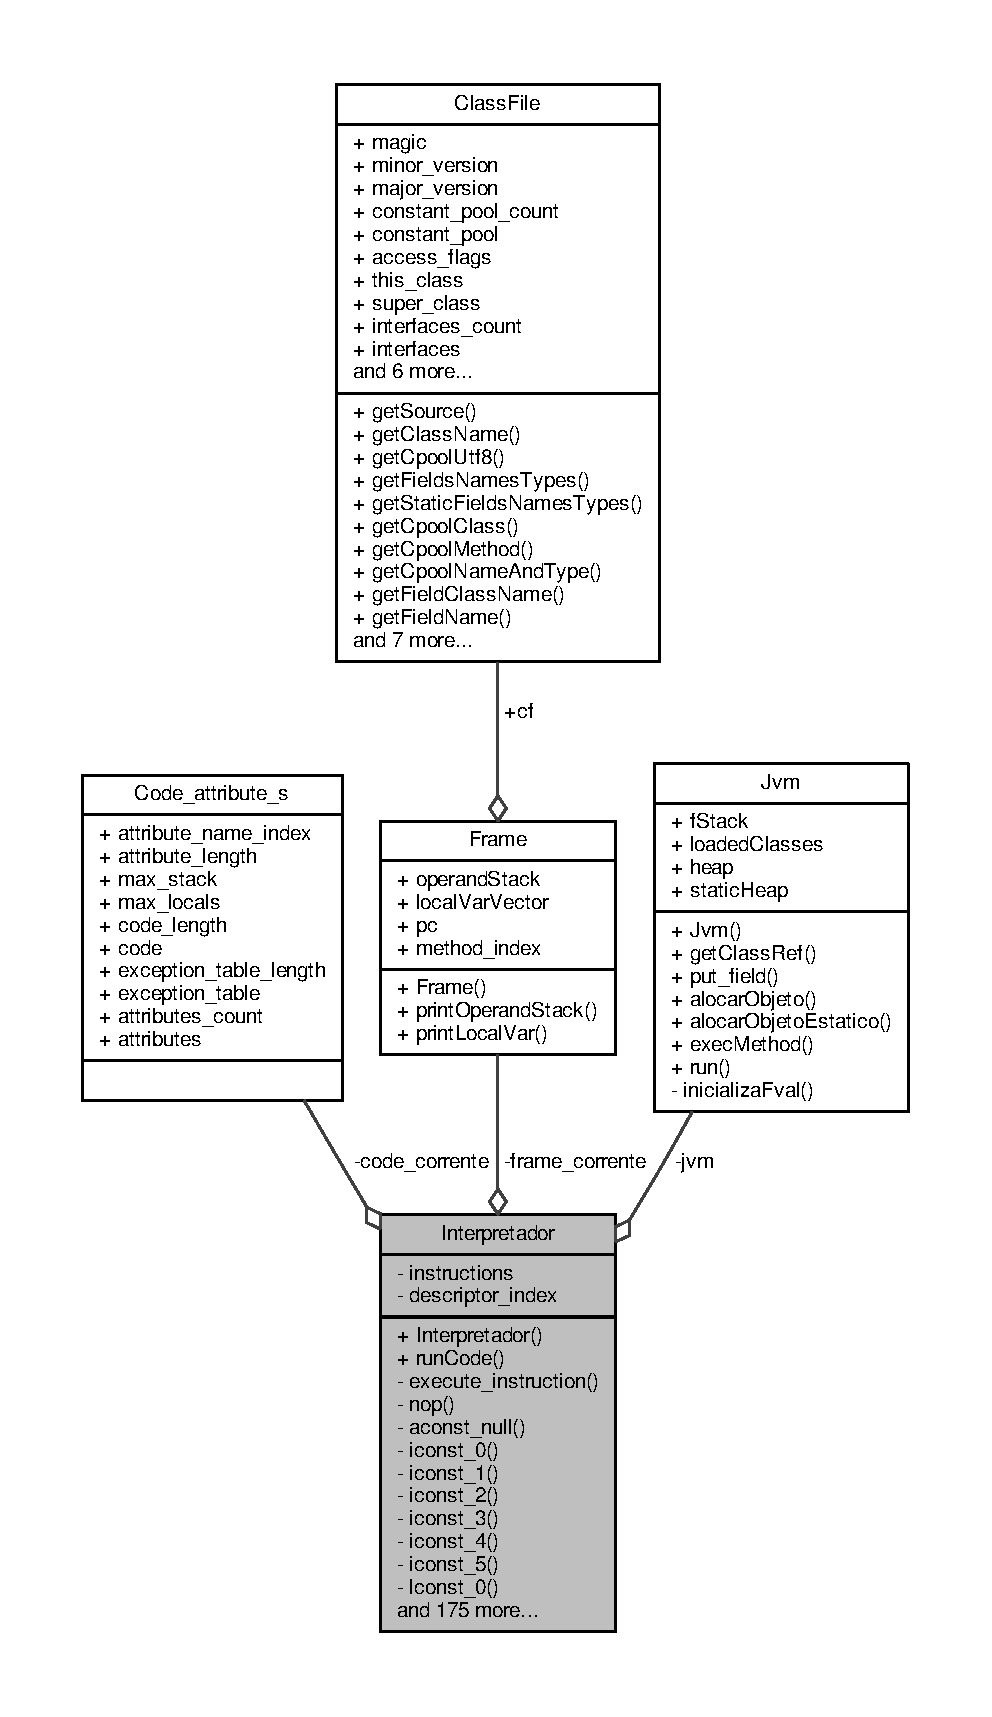
\includegraphics[width=194pt]{classInterpretador__coll__graph}
\end{center}
\end{figure}
\subsection*{Public Member Functions}
\begin{DoxyCompactItemize}
\item 
\hyperlink{classInterpretador_a12d844a7ab8d634e96b57971c9aedd9e}{Interpretador} ()
\item 
void \hyperlink{classInterpretador_a2a8c4a95bc1fa1e6a689059f6f7ecb8c}{execute\+\_\+instruction} (int opcode, \hyperlink{frame_8hpp_a27f9a444058fa5dfb484ef1347edd937}{op\+\_\+stack} $\ast$op\+Stack)
\item 
int \hyperlink{classInterpretador_a0a8a79662aafc9cd4a7a194350c7165c}{push\+\_\+operands} (uint8\+\_\+t opcode, char $\ast$code\+Aligned, \hyperlink{frame_8hpp_a27f9a444058fa5dfb484ef1347edd937}{op\+\_\+stack} $\ast$op\+Stack)
\end{DoxyCompactItemize}
\subsection*{Private Types}
\begin{DoxyCompactItemize}
\item 
typedef void(Interpretador\+::$\ast$ \hyperlink{classInterpretador_aaf603472f241d9de30ebf482cabb1ffc}{instruction\+Function} )(\hyperlink{frame_8hpp_a27f9a444058fa5dfb484ef1347edd937}{op\+\_\+stack} $\ast$)
\item 
typedef int(Interpretador\+::$\ast$ \hyperlink{classInterpretador_a6202f301ed122ef7572356e51333a18c}{instruction\+Function\+Operands} )(char $\ast$, \hyperlink{frame_8hpp_a27f9a444058fa5dfb484ef1347edd937}{op\+\_\+stack} $\ast$)
\end{DoxyCompactItemize}
\subsection*{Private Member Functions}
\begin{DoxyCompactItemize}
\item 
void \hyperlink{classInterpretador_a165915133c412ded3f754ec43121a23b}{iadd} (\hyperlink{frame_8hpp_a27f9a444058fa5dfb484ef1347edd937}{op\+\_\+stack} $\ast$op\+Stack)
\item 
int \hyperlink{classInterpretador_aa5b5ae5978b9f45f629807fa3e10c496}{iadd\+\_\+pusher} (char $\ast$code\+Aligned, \hyperlink{frame_8hpp_a27f9a444058fa5dfb484ef1347edd937}{op\+\_\+stack} $\ast$op\+Stack)
\item 
void \hyperlink{classInterpretador_a448412cfc43f6b5501a0e9a61f9a4e12}{ladd} (\hyperlink{frame_8hpp_a27f9a444058fa5dfb484ef1347edd937}{op\+\_\+stack} $\ast$op\+Stack)
\item 
void \hyperlink{classInterpretador_a5b8ee7fdcf502ad96762f874903b3e05}{new\+\_\+op} (\hyperlink{frame_8hpp_a27f9a444058fa5dfb484ef1347edd937}{op\+\_\+stack} $\ast$op\+Stack)
\item 
int \hyperlink{classInterpretador_a10103aeb6ee4fd69ebf1307043bb6036}{new\+\_\+op\+\_\+pusher} (char $\ast$code\+Aligned, \hyperlink{frame_8hpp_a27f9a444058fa5dfb484ef1347edd937}{op\+\_\+stack} $\ast$op\+Stack)
\end{DoxyCompactItemize}
\subsection*{Private Attributes}
\begin{DoxyCompactItemize}
\item 
\hyperlink{classJvm}{Jvm} $\ast$ \hyperlink{classInterpretador_aed3bd481ff345333414aa70360a94b7c}{jvm}
\item 
std\+::vector$<$ \hyperlink{classInterpretador_aaf603472f241d9de30ebf482cabb1ffc}{instruction\+Function} $>$ \hyperlink{classInterpretador_ad31e757e96232fbfc88637b26263055f}{instructions}
\item 
std\+::vector\\*
$<$ \hyperlink{classInterpretador_a6202f301ed122ef7572356e51333a18c}{instruction\+Function\+Operands} $>$ \hyperlink{classInterpretador_a25ace76ac4d752a224422fadfb550ebf}{operands\+\_\+pusher}
\end{DoxyCompactItemize}


\subsection{Member Typedef Documentation}
\hypertarget{classInterpretador_aaf603472f241d9de30ebf482cabb1ffc}{\index{Interpretador@{Interpretador}!instruction\+Function@{instruction\+Function}}
\index{instruction\+Function@{instruction\+Function}!Interpretador@{Interpretador}}
\subsubsection[{instruction\+Function}]{\setlength{\rightskip}{0pt plus 5cm}typedef void(Interpretador\+::$\ast$ Interpretador\+::instruction\+Function)({\bf op\+\_\+stack} $\ast$)\hspace{0.3cm}{\ttfamily [private]}}}\label{classInterpretador_aaf603472f241d9de30ebf482cabb1ffc}
\hypertarget{classInterpretador_a6202f301ed122ef7572356e51333a18c}{\index{Interpretador@{Interpretador}!instruction\+Function\+Operands@{instruction\+Function\+Operands}}
\index{instruction\+Function\+Operands@{instruction\+Function\+Operands}!Interpretador@{Interpretador}}
\subsubsection[{instruction\+Function\+Operands}]{\setlength{\rightskip}{0pt plus 5cm}typedef int(Interpretador\+::$\ast$ Interpretador\+::instruction\+Function\+Operands)(char $\ast$, {\bf op\+\_\+stack} $\ast$)\hspace{0.3cm}{\ttfamily [private]}}}\label{classInterpretador_a6202f301ed122ef7572356e51333a18c}


\subsection{Constructor \& Destructor Documentation}
\hypertarget{classInterpretador_a12d844a7ab8d634e96b57971c9aedd9e}{\index{Interpretador@{Interpretador}!Interpretador@{Interpretador}}
\index{Interpretador@{Interpretador}!Interpretador@{Interpretador}}
\subsubsection[{Interpretador}]{\setlength{\rightskip}{0pt plus 5cm}Interpretador\+::\+Interpretador (
\begin{DoxyParamCaption}
{}
\end{DoxyParamCaption}
)}}\label{classInterpretador_a12d844a7ab8d634e96b57971c9aedd9e}


\subsection{Member Function Documentation}
\hypertarget{classInterpretador_a2a8c4a95bc1fa1e6a689059f6f7ecb8c}{\index{Interpretador@{Interpretador}!execute\+\_\+instruction@{execute\+\_\+instruction}}
\index{execute\+\_\+instruction@{execute\+\_\+instruction}!Interpretador@{Interpretador}}
\subsubsection[{execute\+\_\+instruction}]{\setlength{\rightskip}{0pt plus 5cm}void Interpretador\+::execute\+\_\+instruction (
\begin{DoxyParamCaption}
\item[{int}]{opcode, }
\item[{{\bf op\+\_\+stack} $\ast$}]{op\+Stack}
\end{DoxyParamCaption}
)}}\label{classInterpretador_a2a8c4a95bc1fa1e6a689059f6f7ecb8c}
\hypertarget{classInterpretador_a165915133c412ded3f754ec43121a23b}{\index{Interpretador@{Interpretador}!iadd@{iadd}}
\index{iadd@{iadd}!Interpretador@{Interpretador}}
\subsubsection[{iadd}]{\setlength{\rightskip}{0pt plus 5cm}void Interpretador\+::iadd (
\begin{DoxyParamCaption}
\item[{{\bf op\+\_\+stack} $\ast$}]{op\+Stack}
\end{DoxyParamCaption}
)\hspace{0.3cm}{\ttfamily [private]}}}\label{classInterpretador_a165915133c412ded3f754ec43121a23b}
\hypertarget{classInterpretador_aa5b5ae5978b9f45f629807fa3e10c496}{\index{Interpretador@{Interpretador}!iadd\+\_\+pusher@{iadd\+\_\+pusher}}
\index{iadd\+\_\+pusher@{iadd\+\_\+pusher}!Interpretador@{Interpretador}}
\subsubsection[{iadd\+\_\+pusher}]{\setlength{\rightskip}{0pt plus 5cm}int Interpretador\+::iadd\+\_\+pusher (
\begin{DoxyParamCaption}
\item[{char $\ast$}]{code\+Aligned, }
\item[{{\bf op\+\_\+stack} $\ast$}]{op\+Stack}
\end{DoxyParamCaption}
)\hspace{0.3cm}{\ttfamily [private]}}}\label{classInterpretador_aa5b5ae5978b9f45f629807fa3e10c496}
\hypertarget{classInterpretador_a448412cfc43f6b5501a0e9a61f9a4e12}{\index{Interpretador@{Interpretador}!ladd@{ladd}}
\index{ladd@{ladd}!Interpretador@{Interpretador}}
\subsubsection[{ladd}]{\setlength{\rightskip}{0pt plus 5cm}void Interpretador\+::ladd (
\begin{DoxyParamCaption}
\item[{{\bf op\+\_\+stack} $\ast$}]{op\+Stack}
\end{DoxyParamCaption}
)\hspace{0.3cm}{\ttfamily [private]}}}\label{classInterpretador_a448412cfc43f6b5501a0e9a61f9a4e12}
\hypertarget{classInterpretador_a5b8ee7fdcf502ad96762f874903b3e05}{\index{Interpretador@{Interpretador}!new\+\_\+op@{new\+\_\+op}}
\index{new\+\_\+op@{new\+\_\+op}!Interpretador@{Interpretador}}
\subsubsection[{new\+\_\+op}]{\setlength{\rightskip}{0pt plus 5cm}void Interpretador\+::new\+\_\+op (
\begin{DoxyParamCaption}
\item[{{\bf op\+\_\+stack} $\ast$}]{op\+Stack}
\end{DoxyParamCaption}
)\hspace{0.3cm}{\ttfamily [private]}}}\label{classInterpretador_a5b8ee7fdcf502ad96762f874903b3e05}
\hypertarget{classInterpretador_a10103aeb6ee4fd69ebf1307043bb6036}{\index{Interpretador@{Interpretador}!new\+\_\+op\+\_\+pusher@{new\+\_\+op\+\_\+pusher}}
\index{new\+\_\+op\+\_\+pusher@{new\+\_\+op\+\_\+pusher}!Interpretador@{Interpretador}}
\subsubsection[{new\+\_\+op\+\_\+pusher}]{\setlength{\rightskip}{0pt plus 5cm}int Interpretador\+::new\+\_\+op\+\_\+pusher (
\begin{DoxyParamCaption}
\item[{char $\ast$}]{code\+Aligned, }
\item[{{\bf op\+\_\+stack} $\ast$}]{op\+Stack}
\end{DoxyParamCaption}
)\hspace{0.3cm}{\ttfamily [private]}}}\label{classInterpretador_a10103aeb6ee4fd69ebf1307043bb6036}
\hypertarget{classInterpretador_a0a8a79662aafc9cd4a7a194350c7165c}{\index{Interpretador@{Interpretador}!push\+\_\+operands@{push\+\_\+operands}}
\index{push\+\_\+operands@{push\+\_\+operands}!Interpretador@{Interpretador}}
\subsubsection[{push\+\_\+operands}]{\setlength{\rightskip}{0pt plus 5cm}int Interpretador\+::push\+\_\+operands (
\begin{DoxyParamCaption}
\item[{uint8\+\_\+t}]{opcode, }
\item[{char $\ast$}]{code\+Aligned, }
\item[{{\bf op\+\_\+stack} $\ast$}]{op\+Stack}
\end{DoxyParamCaption}
)}}\label{classInterpretador_a0a8a79662aafc9cd4a7a194350c7165c}


\subsection{Member Data Documentation}
\hypertarget{classInterpretador_ad31e757e96232fbfc88637b26263055f}{\index{Interpretador@{Interpretador}!instructions@{instructions}}
\index{instructions@{instructions}!Interpretador@{Interpretador}}
\subsubsection[{instructions}]{\setlength{\rightskip}{0pt plus 5cm}std\+::vector$<${\bf instruction\+Function}$>$ Interpretador\+::instructions\hspace{0.3cm}{\ttfamily [private]}}}\label{classInterpretador_ad31e757e96232fbfc88637b26263055f}
\hypertarget{classInterpretador_aed3bd481ff345333414aa70360a94b7c}{\index{Interpretador@{Interpretador}!jvm@{jvm}}
\index{jvm@{jvm}!Interpretador@{Interpretador}}
\subsubsection[{jvm}]{\setlength{\rightskip}{0pt plus 5cm}{\bf Jvm}$\ast$ Interpretador\+::jvm\hspace{0.3cm}{\ttfamily [private]}}}\label{classInterpretador_aed3bd481ff345333414aa70360a94b7c}
\hypertarget{classInterpretador_a25ace76ac4d752a224422fadfb550ebf}{\index{Interpretador@{Interpretador}!operands\+\_\+pusher@{operands\+\_\+pusher}}
\index{operands\+\_\+pusher@{operands\+\_\+pusher}!Interpretador@{Interpretador}}
\subsubsection[{operands\+\_\+pusher}]{\setlength{\rightskip}{0pt plus 5cm}std\+::vector$<${\bf instruction\+Function\+Operands}$>$ Interpretador\+::operands\+\_\+pusher\hspace{0.3cm}{\ttfamily [private]}}}\label{classInterpretador_a25ace76ac4d752a224422fadfb550ebf}


The documentation for this class was generated from the following files\+:\begin{DoxyCompactItemize}
\item 
include/\hyperlink{interpretador_8hpp}{interpretador.\+hpp}\item 
src/\hyperlink{interpretador_8cpp}{interpretador.\+cpp}\end{DoxyCompactItemize}

\hypertarget{classJvm}{\section{Jvm Class Reference}
\label{classJvm}\index{Jvm@{Jvm}}
}


Esta é a classe mãe da J\+V\+M ela Ela quem deve encontrar a main da classe inicial e rodar o loop para rodar os métodos. Ela quem é responsável pela heap, e pela gerencia dos objetos alocados em geral inclusive os classfile!  




{\ttfamily \#include $<$jvm.\+hpp$>$}



Collaboration diagram for Jvm\+:
\nopagebreak
\begin{figure}[H]
\begin{center}
\leavevmode
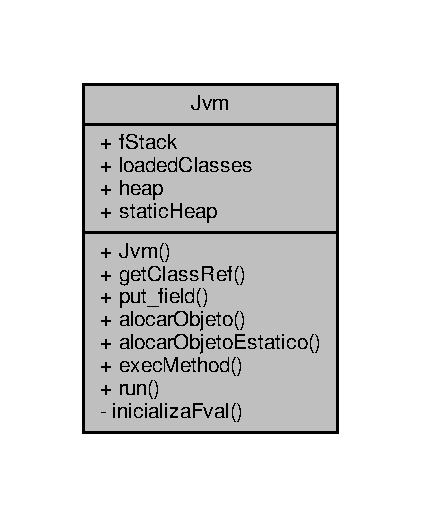
\includegraphics[width=202pt]{classJvm__coll__graph}
\end{center}
\end{figure}
\subsection*{Public Member Functions}
\begin{DoxyCompactItemize}
\item 
\hyperlink{classJvm_a2bbdf6ed1c101825a440bd38dfa54a5a}{Jvm} ()
\item 
\hyperlink{classClassFile}{Class\+File} $\ast$ \hyperlink{classJvm_a6c159c7b6eed436d26b95e4af9fdca87}{get\+Class\+Ref} (std\+::string class\+Name)
\begin{DoxyCompactList}\small\item\em Obtém uma referencia para uma classe carregada. A classe é carregada, caso já não estiver. \end{DoxyCompactList}\item 
void \hyperlink{classJvm_a828e1608fdac86ee26615021e2b63a80}{put\+\_\+field} (std\+::string field\+\_\+name, \hyperlink{classLocal__var}{Local\+\_\+var} lvar)
\begin{DoxyCompactList}\small\item\em Altera o valor de um dado field. \end{DoxyCompactList}\item 
\hyperlink{classInstanceClass}{Instance\+Class} $\ast$ \hyperlink{classJvm_a854b6ba06d1a9187ec7699861c57e3a3}{alocar\+Objeto} (std\+::string class\+Name)
\begin{DoxyCompactList}\small\item\em Carrega a instancia de uma classe carregada, alocando as fields e instanciando com os valores padrão. \end{DoxyCompactList}\item 
\hyperlink{classInstanceClass}{Instance\+Class} $\ast$ \hyperlink{classJvm_a03ab322c195c906da1da0455a4ef794f}{alocar\+Objeto\+Estatico} (std\+::string class\+Name)
\begin{DoxyCompactList}\small\item\em Carrega a instância de uma classe carregada, alocando as fields estaticas e instânciando com os valores padrão. \end{DoxyCompactList}\item 
tuple$<$ \hyperlink{classLocal__var}{Local\+\_\+var}, \hyperlink{classLocal__var}{Local\+\_\+var} $>$ \hyperlink{classJvm_adc00dfd960276f1d115debcf8f0a2a9c}{exec\+Method} (int method\+\_\+index, \hyperlink{classClassFile}{Class\+File} $\ast$class\+F, vector$<$ \hyperlink{classLocal__var}{Local\+\_\+var} $>$ \&jargs)
\begin{DoxyCompactList}\small\item\em executa o metodo de indice method\+\_\+index do vetor de codigo do class\+F \end{DoxyCompactList}\item 
int \hyperlink{classJvm_ac7b36cf9d42be5f4e9fbd1e49f4565d3}{run} (const char $\ast$arq\+\_\+class\+\_\+name)
\begin{DoxyCompactList}\small\item\em carrega o classfile, realiza a verificacao de tipos, verifica se classe carregada possui metodo main caso exista chama o exec\+Method para executa-\/lo. \end{DoxyCompactList}\end{DoxyCompactItemize}
\subsection*{Public Attributes}
\begin{DoxyCompactItemize}
\item 
std\+::vector$<$ \hyperlink{classFrame}{Frame} $>$ \hyperlink{classJvm_ab19406aec3e97ade3d4efbd5796c36f3}{f\+Stack}
\begin{DoxyCompactList}\small\item\em Pilha de execução da jvm. Pilha de frames. \end{DoxyCompactList}\item 
std\+::map$<$ std\+::string, \\*
\hyperlink{classClassFile}{Class\+File} $\ast$ $>$ \hyperlink{classJvm_ac74fb0e170f232ddc32244a1ce7746b7}{loaded\+Classes}
\begin{DoxyCompactList}\small\item\em mapa de classes carregadas. \end{DoxyCompactList}\item 
std\+::vector$<$ \hyperlink{classInstanceClass}{Instance\+Class} $\ast$ $>$ \hyperlink{classJvm_a8e1cdfdf727e1b674a033fbd17337f38}{heap}
\begin{DoxyCompactList}\small\item\em Mapeia classname para instancias. \end{DoxyCompactList}\item 
std\+::map$<$ std\+::string, \\*
\hyperlink{classInstanceClass}{Instance\+Class} $\ast$ $>$ \hyperlink{classJvm_a8852d50533c03dabd4320c27e92d4f1b}{static\+Heap}
\end{DoxyCompactItemize}
\subsection*{Private Member Functions}
\begin{DoxyCompactItemize}
\item 
\hyperlink{classFieldValue}{Field\+Value} \hyperlink{classJvm_a2c1ac5823895df859f9effc95b84d9b0}{inicializa\+Fval} (const char $\ast$ftype, int n)
\begin{DoxyCompactList}\small\item\em Constroi uma \hyperlink{classFieldValue}{Field\+Value} com os valores padroes, a maioria zero ou false para booleanos, ou array com a dimensao certa mas vazio, ou null. \end{DoxyCompactList}\end{DoxyCompactItemize}
\subsection*{Private Attributes}
\begin{DoxyCompactItemize}
\item 
std\+::string \hyperlink{classJvm_acbc46e076119ba010c5434db208b6536}{classpath}
\end{DoxyCompactItemize}


\subsection{Detailed Description}
Esta é a classe mãe da J\+V\+M ela Ela quem deve encontrar a main da classe inicial e rodar o loop para rodar os métodos. Ela quem é responsável pela heap, e pela gerencia dos objetos alocados em geral inclusive os classfile! 

\subsection{Constructor \& Destructor Documentation}
\hypertarget{classJvm_a2bbdf6ed1c101825a440bd38dfa54a5a}{\index{Jvm@{Jvm}!Jvm@{Jvm}}
\index{Jvm@{Jvm}!Jvm@{Jvm}}
\subsubsection[{Jvm}]{\setlength{\rightskip}{0pt plus 5cm}Jvm\+::\+Jvm (
\begin{DoxyParamCaption}
{}
\end{DoxyParamCaption}
)\hspace{0.3cm}{\ttfamily [inline]}}}\label{classJvm_a2bbdf6ed1c101825a440bd38dfa54a5a}


\subsection{Member Function Documentation}
\hypertarget{classJvm_a854b6ba06d1a9187ec7699861c57e3a3}{\index{Jvm@{Jvm}!alocar\+Objeto@{alocar\+Objeto}}
\index{alocar\+Objeto@{alocar\+Objeto}!Jvm@{Jvm}}
\subsubsection[{alocar\+Objeto}]{\setlength{\rightskip}{0pt plus 5cm}{\bf Instance\+Class} $\ast$ Jvm\+::alocar\+Objeto (
\begin{DoxyParamCaption}
\item[{std\+::string}]{class\+Name}
\end{DoxyParamCaption}
)}}\label{classJvm_a854b6ba06d1a9187ec7699861c57e3a3}


Carrega a instancia de uma classe carregada, alocando as fields e instanciando com os valores padrão. 


\begin{DoxyParams}{Parameters}
{\em class\+Name} & nome da classe a ser alocada\\
\hline
\end{DoxyParams}
\begin{DoxyReturn}{Returns}
A referência da instancia da classe alocada com valores padrao. 
\end{DoxyReturn}
\hypertarget{classJvm_a03ab322c195c906da1da0455a4ef794f}{\index{Jvm@{Jvm}!alocar\+Objeto\+Estatico@{alocar\+Objeto\+Estatico}}
\index{alocar\+Objeto\+Estatico@{alocar\+Objeto\+Estatico}!Jvm@{Jvm}}
\subsubsection[{alocar\+Objeto\+Estatico}]{\setlength{\rightskip}{0pt plus 5cm}{\bf Instance\+Class} $\ast$ Jvm\+::alocar\+Objeto\+Estatico (
\begin{DoxyParamCaption}
\item[{std\+::string}]{class\+Name}
\end{DoxyParamCaption}
)}}\label{classJvm_a03ab322c195c906da1da0455a4ef794f}


Carrega a instância de uma classe carregada, alocando as fields estaticas e instânciando com os valores padrão. 


\begin{DoxyParams}{Parameters}
{\em class\+Name} & nome da classe a ser alocada\\
\hline
\end{DoxyParams}
\begin{DoxyReturn}{Returns}
A referencia da instância da classe estatica alocada com valores padrao. 
\end{DoxyReturn}
\hypertarget{classJvm_adc00dfd960276f1d115debcf8f0a2a9c}{\index{Jvm@{Jvm}!exec\+Method@{exec\+Method}}
\index{exec\+Method@{exec\+Method}!Jvm@{Jvm}}
\subsubsection[{exec\+Method}]{\setlength{\rightskip}{0pt plus 5cm}tuple$<$ {\bf Local\+\_\+var}, {\bf Local\+\_\+var} $>$ Jvm\+::exec\+Method (
\begin{DoxyParamCaption}
\item[{int}]{method\+\_\+index, }
\item[{{\bf Class\+File} $\ast$}]{class\+F, }
\item[{vector$<$ {\bf Local\+\_\+var} $>$ \&}]{args}
\end{DoxyParamCaption}
)}}\label{classJvm_adc00dfd960276f1d115debcf8f0a2a9c}


executa o metodo de indice method\+\_\+index do vetor de codigo do class\+F 


\begin{DoxyParams}{Parameters}
{\em method\+\_\+index} & o indice do método na class\+F a ser executado \\
\hline
{\em class\+F} & é o ponteiro para o \hyperlink{classClassFile}{Class\+File} dono do método a ser executado \\
\hline
{\em jargs} & são os parametros que serao passado como argumento\\
\hline
\end{DoxyParams}
\begin{DoxyReturn}{Returns}
o retorno do metodo empacotado numa \hyperlink{classLocal__var}{Local\+\_\+var}
\end{DoxyReturn}
exec\+Method é criar o ambiente para que o método possa ser executado\+: inicializa as informações no frame; encontra e prepara method para execução; encontra o índice do descritor do metodo. \hypertarget{classJvm_a6c159c7b6eed436d26b95e4af9fdca87}{\index{Jvm@{Jvm}!get\+Class\+Ref@{get\+Class\+Ref}}
\index{get\+Class\+Ref@{get\+Class\+Ref}!Jvm@{Jvm}}
\subsubsection[{get\+Class\+Ref}]{\setlength{\rightskip}{0pt plus 5cm}{\bf Class\+File} $\ast$ Jvm\+::get\+Class\+Ref (
\begin{DoxyParamCaption}
\item[{std\+::string}]{class\+Name}
\end{DoxyParamCaption}
)}}\label{classJvm_a6c159c7b6eed436d26b95e4af9fdca87}


Obtém uma referencia para uma classe carregada. A classe é carregada, caso já não estiver. 


\begin{DoxyParams}{Parameters}
{\em class\+Name} & nome da classe a ser retornada\\
\hline
\end{DoxyParams}
\begin{DoxyReturn}{Returns}
A classfile que de fato representa a estrutura do .class 
\end{DoxyReturn}
\hypertarget{classJvm_a2c1ac5823895df859f9effc95b84d9b0}{\index{Jvm@{Jvm}!inicializa\+Fval@{inicializa\+Fval}}
\index{inicializa\+Fval@{inicializa\+Fval}!Jvm@{Jvm}}
\subsubsection[{inicializa\+Fval}]{\setlength{\rightskip}{0pt plus 5cm}{\bf Field\+Value} Jvm\+::inicializa\+Fval (
\begin{DoxyParamCaption}
\item[{const char $\ast$}]{ftype, }
\item[{int}]{n}
\end{DoxyParamCaption}
)\hspace{0.3cm}{\ttfamily [private]}}}\label{classJvm_a2c1ac5823895df859f9effc95b84d9b0}


Constroi uma \hyperlink{classFieldValue}{Field\+Value} com os valores padroes, a maioria zero ou false para booleanos, ou array com a dimensao certa mas vazio, ou null. 


\begin{DoxyParams}{Parameters}
{\em ftype} & eh o descritor da field \\
\hline
{\em n} & parametro para recursao, chame esta funcao passando como valor inicial sempre zero.\\
\hline
\end{DoxyParams}
\begin{DoxyReturn}{Returns}
uma \hyperlink{classFieldValue}{Field\+Value} inicializada 
\end{DoxyReturn}
\hypertarget{classJvm_a828e1608fdac86ee26615021e2b63a80}{\index{Jvm@{Jvm}!put\+\_\+field@{put\+\_\+field}}
\index{put\+\_\+field@{put\+\_\+field}!Jvm@{Jvm}}
\subsubsection[{put\+\_\+field}]{\setlength{\rightskip}{0pt plus 5cm}void Jvm\+::put\+\_\+field (
\begin{DoxyParamCaption}
\item[{std\+::string}]{field\+\_\+name, }
\item[{{\bf Local\+\_\+var}}]{lvar}
\end{DoxyParamCaption}
)}}\label{classJvm_a828e1608fdac86ee26615021e2b63a80}


Altera o valor de um dado field. 


\begin{DoxyParams}{Parameters}
{\em field\+\_\+name} & nome do field a ser alterado \\
\hline
{\em lvar} & valor para colocar no field\\
\hline
\end{DoxyParams}
\begin{DoxyReturn}{Returns}
void 
\end{DoxyReturn}
\hypertarget{classJvm_ac7b36cf9d42be5f4e9fbd1e49f4565d3}{\index{Jvm@{Jvm}!run@{run}}
\index{run@{run}!Jvm@{Jvm}}
\subsubsection[{run}]{\setlength{\rightskip}{0pt plus 5cm}int Jvm\+::run (
\begin{DoxyParamCaption}
\item[{const char $\ast$}]{arq\+\_\+class\+\_\+name}
\end{DoxyParamCaption}
)}}\label{classJvm_ac7b36cf9d42be5f4e9fbd1e49f4565d3}


carrega o classfile, realiza a verificacao de tipos, verifica se classe carregada possui metodo main caso exista chama o exec\+Method para executa-\/lo. 


\begin{DoxyParams}{Parameters}
{\em arq\+\_\+class\+\_\+name} & nome do arquivo com o bytecode a ser lido\\
\hline
\end{DoxyParams}
\begin{DoxyReturn}{Returns}
o retorno e sempre 0 
\end{DoxyReturn}


\subsection{Member Data Documentation}
\hypertarget{classJvm_acbc46e076119ba010c5434db208b6536}{\index{Jvm@{Jvm}!classpath@{classpath}}
\index{classpath@{classpath}!Jvm@{Jvm}}
\subsubsection[{classpath}]{\setlength{\rightskip}{0pt plus 5cm}O class principal encontra se em um Jvm\+::classpath\hspace{0.3cm}{\ttfamily [private]}}}\label{classJvm_acbc46e076119ba010c5434db208b6536}
todos próximos arquivos serão procurados na mesma pasta que o programa ou dentro deste classpath. \hypertarget{classJvm_ab19406aec3e97ade3d4efbd5796c36f3}{\index{Jvm@{Jvm}!f\+Stack@{f\+Stack}}
\index{f\+Stack@{f\+Stack}!Jvm@{Jvm}}
\subsubsection[{f\+Stack}]{\setlength{\rightskip}{0pt plus 5cm}Jvm\+::f\+Stack}}\label{classJvm_ab19406aec3e97ade3d4efbd5796c36f3}


Pilha de execução da jvm. Pilha de frames. 

\hypertarget{classJvm_a8e1cdfdf727e1b674a033fbd17337f38}{\index{Jvm@{Jvm}!heap@{heap}}
\index{heap@{heap}!Jvm@{Jvm}}
\subsubsection[{heap}]{\setlength{\rightskip}{0pt plus 5cm}static Jvm\+::heap}}\label{classJvm_a8e1cdfdf727e1b674a033fbd17337f38}


Mapeia classname para instancias. 

Mapeia classname para os nomes e valores de seus fields estaticos. \hypertarget{classJvm_ac74fb0e170f232ddc32244a1ce7746b7}{\index{Jvm@{Jvm}!loaded\+Classes@{loaded\+Classes}}
\index{loaded\+Classes@{loaded\+Classes}!Jvm@{Jvm}}
\subsubsection[{loaded\+Classes}]{\setlength{\rightskip}{0pt plus 5cm}std\+::map$<$ std\+::string, {\bf Class\+File} $>$ Jvm\+::loaded\+Classes}}\label{classJvm_ac74fb0e170f232ddc32244a1ce7746b7}


mapa de classes carregadas. 

\hypertarget{classJvm_a8852d50533c03dabd4320c27e92d4f1b}{\index{Jvm@{Jvm}!static\+Heap@{static\+Heap}}
\index{static\+Heap@{static\+Heap}!Jvm@{Jvm}}
\subsubsection[{static\+Heap}]{\setlength{\rightskip}{0pt plus 5cm}std\+::map$<$std\+::string, {\bf Instance\+Class}$\ast$$>$ Jvm\+::static\+Heap}}\label{classJvm_a8852d50533c03dabd4320c27e92d4f1b}


The documentation for this class was generated from the following files\+:\begin{DoxyCompactItemize}
\item 
include/\hyperlink{jvm_8hpp}{jvm.\+hpp}\item 
src/\hyperlink{jvm_8cpp}{jvm.\+cpp}\end{DoxyCompactItemize}

\hypertarget{structline__number__table__info__s}{\section{line\+\_\+number\+\_\+table\+\_\+info\+\_\+s Struct Reference}
\label{structline__number__table__info__s}\index{line\+\_\+number\+\_\+table\+\_\+info\+\_\+s@{line\+\_\+number\+\_\+table\+\_\+info\+\_\+s}}
}


{\ttfamily \#include $<$attributes.\+hpp$>$}



Collaboration diagram for line\+\_\+number\+\_\+table\+\_\+info\+\_\+s\+:\nopagebreak
\begin{figure}[H]
\begin{center}
\leavevmode
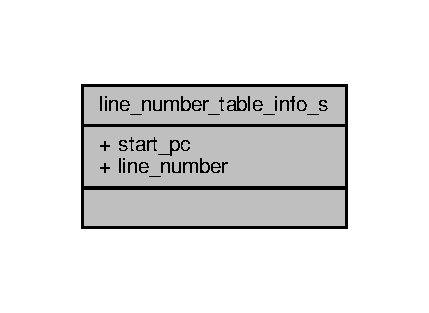
\includegraphics[width=206pt]{structline__number__table__info__s__coll__graph}
\end{center}
\end{figure}
\subsection*{Public Attributes}
\begin{DoxyCompactItemize}
\item 
uint16\+\_\+t \hyperlink{structline__number__table__info__s_ac18154b426adb423127cd7f09c037424}{start\+\_\+pc}
\item 
uint16\+\_\+t \hyperlink{structline__number__table__info__s_ad953dc84b13bcebcee8b877afc6fdcab}{line\+\_\+number}
\end{DoxyCompactItemize}


\subsection{Member Data Documentation}
\hypertarget{structline__number__table__info__s_ad953dc84b13bcebcee8b877afc6fdcab}{\index{line\+\_\+number\+\_\+table\+\_\+info\+\_\+s@{line\+\_\+number\+\_\+table\+\_\+info\+\_\+s}!line\+\_\+number@{line\+\_\+number}}
\index{line\+\_\+number@{line\+\_\+number}!line\+\_\+number\+\_\+table\+\_\+info\+\_\+s@{line\+\_\+number\+\_\+table\+\_\+info\+\_\+s}}
\subsubsection[{line\+\_\+number}]{\setlength{\rightskip}{0pt plus 5cm}uint16\+\_\+t line\+\_\+number\+\_\+table\+\_\+info\+\_\+s\+::line\+\_\+number}}\label{structline__number__table__info__s_ad953dc84b13bcebcee8b877afc6fdcab}
\hypertarget{structline__number__table__info__s_ac18154b426adb423127cd7f09c037424}{\index{line\+\_\+number\+\_\+table\+\_\+info\+\_\+s@{line\+\_\+number\+\_\+table\+\_\+info\+\_\+s}!start\+\_\+pc@{start\+\_\+pc}}
\index{start\+\_\+pc@{start\+\_\+pc}!line\+\_\+number\+\_\+table\+\_\+info\+\_\+s@{line\+\_\+number\+\_\+table\+\_\+info\+\_\+s}}
\subsubsection[{start\+\_\+pc}]{\setlength{\rightskip}{0pt plus 5cm}uint16\+\_\+t line\+\_\+number\+\_\+table\+\_\+info\+\_\+s\+::start\+\_\+pc}}\label{structline__number__table__info__s_ac18154b426adb423127cd7f09c037424}


The documentation for this struct was generated from the following file\+:\begin{DoxyCompactItemize}
\item 
include/\hyperlink{attributes_8hpp}{attributes.\+hpp}\end{DoxyCompactItemize}

\hypertarget{structLineNumberTable__attribute__s}{\section{Line\+Number\+Table\+\_\+attribute\+\_\+s Struct Reference}
\label{structLineNumberTable__attribute__s}\index{Line\+Number\+Table\+\_\+attribute\+\_\+s@{Line\+Number\+Table\+\_\+attribute\+\_\+s}}
}


{\ttfamily \#include $<$attributes.\+hpp$>$}



Collaboration diagram for Line\+Number\+Table\+\_\+attribute\+\_\+s\+:\nopagebreak
\begin{figure}[H]
\begin{center}
\leavevmode
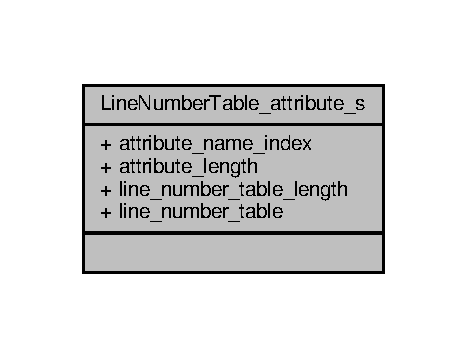
\includegraphics[width=224pt]{structLineNumberTable__attribute__s__coll__graph}
\end{center}
\end{figure}
\subsection*{Public Attributes}
\begin{DoxyCompactItemize}
\item 
uint16\+\_\+t \hyperlink{structLineNumberTable__attribute__s_aac15efe1c90438dc07107171766d8637}{attribute\+\_\+name\+\_\+index}
\item 
uint32\+\_\+t \hyperlink{structLineNumberTable__attribute__s_ab542a17d507ee228ba3967068a20f990}{attribute\+\_\+length}
\item 
uint16\+\_\+t \hyperlink{structLineNumberTable__attribute__s_af17b7841355aa53d48fbfe84e34729c5}{line\+\_\+number\+\_\+table\+\_\+length}
\item 
std\+::vector\\*
$<$ \hyperlink{attributes_8hpp_a27b6c85369a912aa549462c1ede3cc99}{line\+\_\+number\+\_\+table\+\_\+info} $>$ $\ast$ \hyperlink{structLineNumberTable__attribute__s_a434f6fcd9cf968392ae7b9436c118e93}{line\+\_\+number\+\_\+table}
\end{DoxyCompactItemize}


\subsection{Member Data Documentation}
\hypertarget{structLineNumberTable__attribute__s_ab542a17d507ee228ba3967068a20f990}{\index{Line\+Number\+Table\+\_\+attribute\+\_\+s@{Line\+Number\+Table\+\_\+attribute\+\_\+s}!attribute\+\_\+length@{attribute\+\_\+length}}
\index{attribute\+\_\+length@{attribute\+\_\+length}!Line\+Number\+Table\+\_\+attribute\+\_\+s@{Line\+Number\+Table\+\_\+attribute\+\_\+s}}
\subsubsection[{attribute\+\_\+length}]{\setlength{\rightskip}{0pt plus 5cm}uint32\+\_\+t Line\+Number\+Table\+\_\+attribute\+\_\+s\+::attribute\+\_\+length}}\label{structLineNumberTable__attribute__s_ab542a17d507ee228ba3967068a20f990}
\hypertarget{structLineNumberTable__attribute__s_aac15efe1c90438dc07107171766d8637}{\index{Line\+Number\+Table\+\_\+attribute\+\_\+s@{Line\+Number\+Table\+\_\+attribute\+\_\+s}!attribute\+\_\+name\+\_\+index@{attribute\+\_\+name\+\_\+index}}
\index{attribute\+\_\+name\+\_\+index@{attribute\+\_\+name\+\_\+index}!Line\+Number\+Table\+\_\+attribute\+\_\+s@{Line\+Number\+Table\+\_\+attribute\+\_\+s}}
\subsubsection[{attribute\+\_\+name\+\_\+index}]{\setlength{\rightskip}{0pt plus 5cm}uint16\+\_\+t Line\+Number\+Table\+\_\+attribute\+\_\+s\+::attribute\+\_\+name\+\_\+index}}\label{structLineNumberTable__attribute__s_aac15efe1c90438dc07107171766d8637}
\hypertarget{structLineNumberTable__attribute__s_a434f6fcd9cf968392ae7b9436c118e93}{\index{Line\+Number\+Table\+\_\+attribute\+\_\+s@{Line\+Number\+Table\+\_\+attribute\+\_\+s}!line\+\_\+number\+\_\+table@{line\+\_\+number\+\_\+table}}
\index{line\+\_\+number\+\_\+table@{line\+\_\+number\+\_\+table}!Line\+Number\+Table\+\_\+attribute\+\_\+s@{Line\+Number\+Table\+\_\+attribute\+\_\+s}}
\subsubsection[{line\+\_\+number\+\_\+table}]{\setlength{\rightskip}{0pt plus 5cm}std\+::vector$<${\bf line\+\_\+number\+\_\+table\+\_\+info}$>$$\ast$ Line\+Number\+Table\+\_\+attribute\+\_\+s\+::line\+\_\+number\+\_\+table}}\label{structLineNumberTable__attribute__s_a434f6fcd9cf968392ae7b9436c118e93}
\hypertarget{structLineNumberTable__attribute__s_af17b7841355aa53d48fbfe84e34729c5}{\index{Line\+Number\+Table\+\_\+attribute\+\_\+s@{Line\+Number\+Table\+\_\+attribute\+\_\+s}!line\+\_\+number\+\_\+table\+\_\+length@{line\+\_\+number\+\_\+table\+\_\+length}}
\index{line\+\_\+number\+\_\+table\+\_\+length@{line\+\_\+number\+\_\+table\+\_\+length}!Line\+Number\+Table\+\_\+attribute\+\_\+s@{Line\+Number\+Table\+\_\+attribute\+\_\+s}}
\subsubsection[{line\+\_\+number\+\_\+table\+\_\+length}]{\setlength{\rightskip}{0pt plus 5cm}uint16\+\_\+t Line\+Number\+Table\+\_\+attribute\+\_\+s\+::line\+\_\+number\+\_\+table\+\_\+length}}\label{structLineNumberTable__attribute__s_af17b7841355aa53d48fbfe84e34729c5}


The documentation for this struct was generated from the following file\+:\begin{DoxyCompactItemize}
\item 
include/\hyperlink{attributes_8hpp}{attributes.\+hpp}\end{DoxyCompactItemize}

\hypertarget{structlocal__var__s}{\section{local\+\_\+var\+\_\+s Struct Reference}
\label{structlocal__var__s}\index{local\+\_\+var\+\_\+s@{local\+\_\+var\+\_\+s}}
}


{\ttfamily \#include $<$frame.\+hpp$>$}



Collaboration diagram for local\+\_\+var\+\_\+s\+:\nopagebreak
\begin{figure}[H]
\begin{center}
\leavevmode
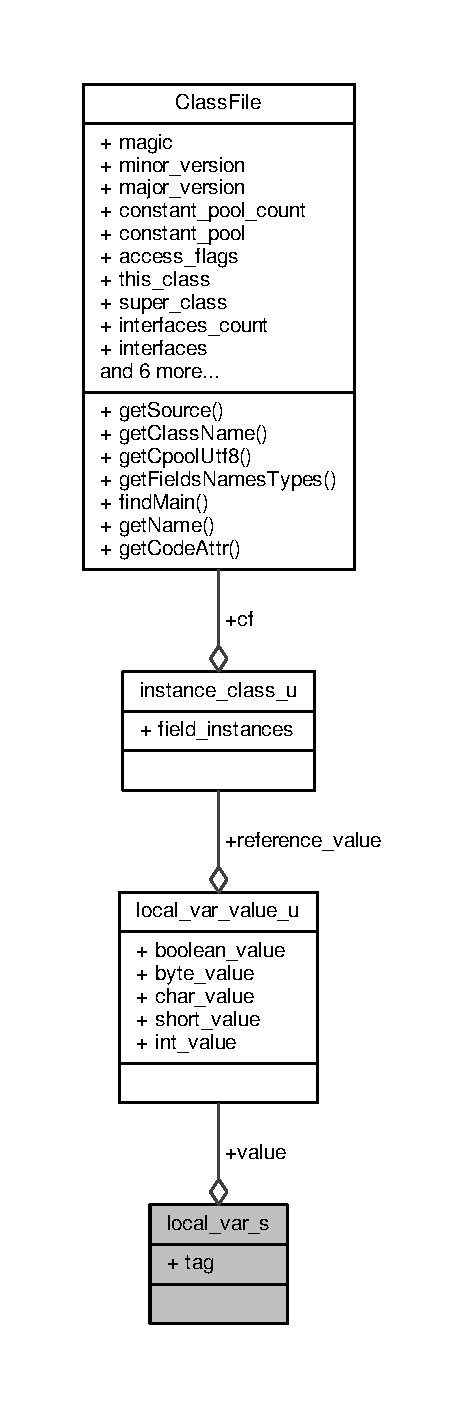
\includegraphics[height=550pt]{structlocal__var__s__coll__graph}
\end{center}
\end{figure}
\subsection*{Public Attributes}
\begin{DoxyCompactItemize}
\item 
uint8\+\_\+t \hyperlink{structlocal__var__s_ab6da81466316f0fcec86450b154b2278}{tag}
\item 
\hyperlink{frame_8hpp_a4dcc6b91c94454a3d19452e6c1353533}{local\+\_\+var\+\_\+value} \hyperlink{structlocal__var__s_a5f2837a0cc5caf9a0b74f2f8745a0164}{value}
\end{DoxyCompactItemize}


\subsection{Member Data Documentation}
\hypertarget{structlocal__var__s_ab6da81466316f0fcec86450b154b2278}{\index{local\+\_\+var\+\_\+s@{local\+\_\+var\+\_\+s}!tag@{tag}}
\index{tag@{tag}!local\+\_\+var\+\_\+s@{local\+\_\+var\+\_\+s}}
\subsubsection[{tag}]{\setlength{\rightskip}{0pt plus 5cm}uint8\+\_\+t local\+\_\+var\+\_\+s\+::tag}}\label{structlocal__var__s_ab6da81466316f0fcec86450b154b2278}
\hypertarget{structlocal__var__s_a5f2837a0cc5caf9a0b74f2f8745a0164}{\index{local\+\_\+var\+\_\+s@{local\+\_\+var\+\_\+s}!value@{value}}
\index{value@{value}!local\+\_\+var\+\_\+s@{local\+\_\+var\+\_\+s}}
\subsubsection[{value}]{\setlength{\rightskip}{0pt plus 5cm}{\bf local\+\_\+var\+\_\+value} local\+\_\+var\+\_\+s\+::value}}\label{structlocal__var__s_a5f2837a0cc5caf9a0b74f2f8745a0164}


The documentation for this struct was generated from the following file\+:\begin{DoxyCompactItemize}
\item 
include/\hyperlink{frame_8hpp}{frame.\+hpp}\end{DoxyCompactItemize}

\hypertarget{unionlocal__var__value__u}{\section{local\+\_\+var\+\_\+value\+\_\+u Union Reference}
\label{unionlocal__var__value__u}\index{local\+\_\+var\+\_\+value\+\_\+u@{local\+\_\+var\+\_\+value\+\_\+u}}
}


{\ttfamily \#include $<$frame.\+hpp$>$}



Collaboration diagram for local\+\_\+var\+\_\+value\+\_\+u\+:\nopagebreak
\begin{figure}[H]
\begin{center}
\leavevmode
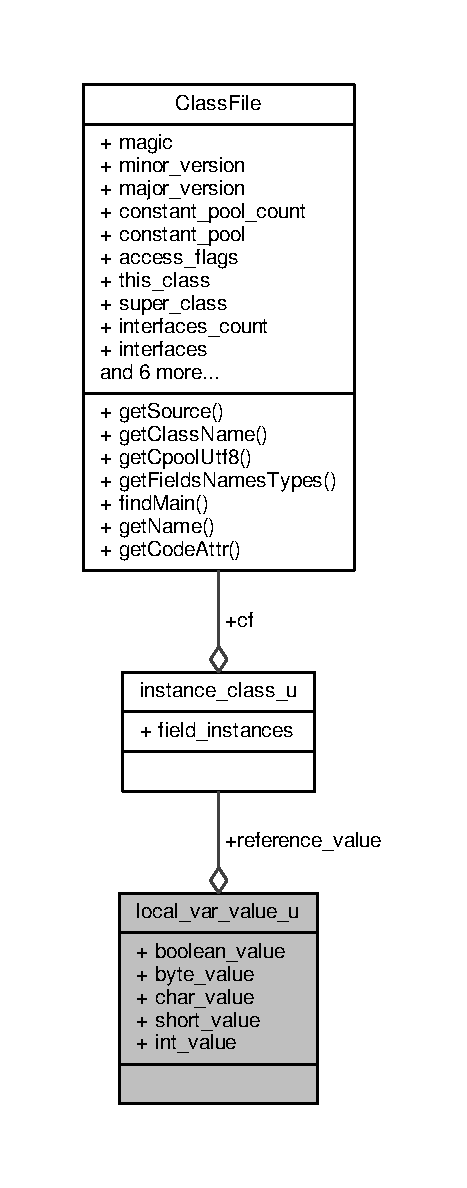
\includegraphics[height=550pt]{unionlocal__var__value__u__coll__graph}
\end{center}
\end{figure}
\subsection*{Public Attributes}
\begin{DoxyCompactItemize}
\item 
bool \hyperlink{unionlocal__var__value__u_a505f55d965d3166fd656c015541b5058}{boolean\+\_\+value}
\item 
uint8\+\_\+t \hyperlink{unionlocal__var__value__u_aa7f181e30d20b090a62375ff58252e5e}{byte\+\_\+value}
\item 
uint8\+\_\+t \hyperlink{unionlocal__var__value__u_a7607fa3be1d65b6c4edc1d350144c4a3}{char\+\_\+value}
\item 
int16\+\_\+t \hyperlink{unionlocal__var__value__u_ae5207df7130db21c87531c1fcdd331d4}{short\+\_\+value}
\item 
int32\+\_\+t \hyperlink{unionlocal__var__value__u_a3d2c83971643d224cbc92c304a5006d4}{int\+\_\+value}
\item 
\hyperlink{heap_8hpp_a10a6b663306bb9ebfa5959ab91c79eda}{Instance\+Class} $\ast$ \hyperlink{unionlocal__var__value__u_a90faf60bf18d81fb6caa6fbe26eca949}{reference\+\_\+value}
\end{DoxyCompactItemize}


\subsection{Member Data Documentation}
\hypertarget{unionlocal__var__value__u_a505f55d965d3166fd656c015541b5058}{\index{local\+\_\+var\+\_\+value\+\_\+u@{local\+\_\+var\+\_\+value\+\_\+u}!boolean\+\_\+value@{boolean\+\_\+value}}
\index{boolean\+\_\+value@{boolean\+\_\+value}!local\+\_\+var\+\_\+value\+\_\+u@{local\+\_\+var\+\_\+value\+\_\+u}}
\subsubsection[{boolean\+\_\+value}]{\setlength{\rightskip}{0pt plus 5cm}bool local\+\_\+var\+\_\+value\+\_\+u\+::boolean\+\_\+value}}\label{unionlocal__var__value__u_a505f55d965d3166fd656c015541b5058}
\hypertarget{unionlocal__var__value__u_aa7f181e30d20b090a62375ff58252e5e}{\index{local\+\_\+var\+\_\+value\+\_\+u@{local\+\_\+var\+\_\+value\+\_\+u}!byte\+\_\+value@{byte\+\_\+value}}
\index{byte\+\_\+value@{byte\+\_\+value}!local\+\_\+var\+\_\+value\+\_\+u@{local\+\_\+var\+\_\+value\+\_\+u}}
\subsubsection[{byte\+\_\+value}]{\setlength{\rightskip}{0pt plus 5cm}uint8\+\_\+t local\+\_\+var\+\_\+value\+\_\+u\+::byte\+\_\+value}}\label{unionlocal__var__value__u_aa7f181e30d20b090a62375ff58252e5e}
\hypertarget{unionlocal__var__value__u_a7607fa3be1d65b6c4edc1d350144c4a3}{\index{local\+\_\+var\+\_\+value\+\_\+u@{local\+\_\+var\+\_\+value\+\_\+u}!char\+\_\+value@{char\+\_\+value}}
\index{char\+\_\+value@{char\+\_\+value}!local\+\_\+var\+\_\+value\+\_\+u@{local\+\_\+var\+\_\+value\+\_\+u}}
\subsubsection[{char\+\_\+value}]{\setlength{\rightskip}{0pt plus 5cm}uint8\+\_\+t local\+\_\+var\+\_\+value\+\_\+u\+::char\+\_\+value}}\label{unionlocal__var__value__u_a7607fa3be1d65b6c4edc1d350144c4a3}
\hypertarget{unionlocal__var__value__u_a3d2c83971643d224cbc92c304a5006d4}{\index{local\+\_\+var\+\_\+value\+\_\+u@{local\+\_\+var\+\_\+value\+\_\+u}!int\+\_\+value@{int\+\_\+value}}
\index{int\+\_\+value@{int\+\_\+value}!local\+\_\+var\+\_\+value\+\_\+u@{local\+\_\+var\+\_\+value\+\_\+u}}
\subsubsection[{int\+\_\+value}]{\setlength{\rightskip}{0pt plus 5cm}int32\+\_\+t local\+\_\+var\+\_\+value\+\_\+u\+::int\+\_\+value}}\label{unionlocal__var__value__u_a3d2c83971643d224cbc92c304a5006d4}
\hypertarget{unionlocal__var__value__u_a90faf60bf18d81fb6caa6fbe26eca949}{\index{local\+\_\+var\+\_\+value\+\_\+u@{local\+\_\+var\+\_\+value\+\_\+u}!reference\+\_\+value@{reference\+\_\+value}}
\index{reference\+\_\+value@{reference\+\_\+value}!local\+\_\+var\+\_\+value\+\_\+u@{local\+\_\+var\+\_\+value\+\_\+u}}
\subsubsection[{reference\+\_\+value}]{\setlength{\rightskip}{0pt plus 5cm}{\bf Instance\+Class}$\ast$ local\+\_\+var\+\_\+value\+\_\+u\+::reference\+\_\+value}}\label{unionlocal__var__value__u_a90faf60bf18d81fb6caa6fbe26eca949}
\hypertarget{unionlocal__var__value__u_ae5207df7130db21c87531c1fcdd331d4}{\index{local\+\_\+var\+\_\+value\+\_\+u@{local\+\_\+var\+\_\+value\+\_\+u}!short\+\_\+value@{short\+\_\+value}}
\index{short\+\_\+value@{short\+\_\+value}!local\+\_\+var\+\_\+value\+\_\+u@{local\+\_\+var\+\_\+value\+\_\+u}}
\subsubsection[{short\+\_\+value}]{\setlength{\rightskip}{0pt plus 5cm}int16\+\_\+t local\+\_\+var\+\_\+value\+\_\+u\+::short\+\_\+value}}\label{unionlocal__var__value__u_ae5207df7130db21c87531c1fcdd331d4}


The documentation for this union was generated from the following file\+:\begin{DoxyCompactItemize}
\item 
include/\hyperlink{frame_8hpp}{frame.\+hpp}\end{DoxyCompactItemize}

\hypertarget{structlocal__variable__table__info__s}{\section{local\+\_\+variable\+\_\+table\+\_\+info\+\_\+s Struct Reference}
\label{structlocal__variable__table__info__s}\index{local\+\_\+variable\+\_\+table\+\_\+info\+\_\+s@{local\+\_\+variable\+\_\+table\+\_\+info\+\_\+s}}
}


{\ttfamily \#include $<$attributes.\+hpp$>$}



Collaboration diagram for local\+\_\+variable\+\_\+table\+\_\+info\+\_\+s\+:\nopagebreak
\begin{figure}[H]
\begin{center}
\leavevmode
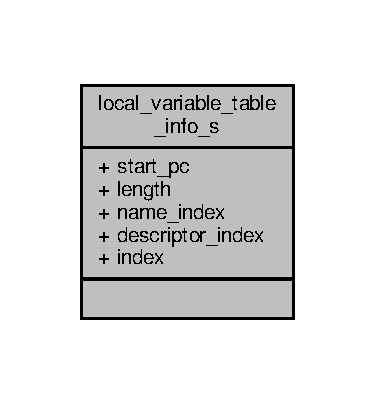
\includegraphics[width=180pt]{structlocal__variable__table__info__s__coll__graph}
\end{center}
\end{figure}
\subsection*{Public Attributes}
\begin{DoxyCompactItemize}
\item 
uint16\+\_\+t \hyperlink{structlocal__variable__table__info__s_a1acd5397525801c3fd91411f647e899c}{start\+\_\+pc}
\item 
uint16\+\_\+t \hyperlink{structlocal__variable__table__info__s_a538a35225c4c1c2c3a32df0f980ef33a}{length}
\item 
uint16\+\_\+t \hyperlink{structlocal__variable__table__info__s_a353fe8c7dceb360da703a4079712692e}{name\+\_\+index}
\item 
uint16\+\_\+t \hyperlink{structlocal__variable__table__info__s_a93d5eda8b9de1714e238dd69cd0db2d5}{descriptor\+\_\+index}
\item 
uint16\+\_\+t \hyperlink{structlocal__variable__table__info__s_a53c64633d6eb65d829cf83b1e344e2b7}{index}
\end{DoxyCompactItemize}


\subsection{Member Data Documentation}
\hypertarget{structlocal__variable__table__info__s_a93d5eda8b9de1714e238dd69cd0db2d5}{\index{local\+\_\+variable\+\_\+table\+\_\+info\+\_\+s@{local\+\_\+variable\+\_\+table\+\_\+info\+\_\+s}!descriptor\+\_\+index@{descriptor\+\_\+index}}
\index{descriptor\+\_\+index@{descriptor\+\_\+index}!local\+\_\+variable\+\_\+table\+\_\+info\+\_\+s@{local\+\_\+variable\+\_\+table\+\_\+info\+\_\+s}}
\subsubsection[{descriptor\+\_\+index}]{\setlength{\rightskip}{0pt plus 5cm}uint16\+\_\+t local\+\_\+variable\+\_\+table\+\_\+info\+\_\+s\+::descriptor\+\_\+index}}\label{structlocal__variable__table__info__s_a93d5eda8b9de1714e238dd69cd0db2d5}
\hypertarget{structlocal__variable__table__info__s_a53c64633d6eb65d829cf83b1e344e2b7}{\index{local\+\_\+variable\+\_\+table\+\_\+info\+\_\+s@{local\+\_\+variable\+\_\+table\+\_\+info\+\_\+s}!index@{index}}
\index{index@{index}!local\+\_\+variable\+\_\+table\+\_\+info\+\_\+s@{local\+\_\+variable\+\_\+table\+\_\+info\+\_\+s}}
\subsubsection[{index}]{\setlength{\rightskip}{0pt plus 5cm}uint16\+\_\+t local\+\_\+variable\+\_\+table\+\_\+info\+\_\+s\+::index}}\label{structlocal__variable__table__info__s_a53c64633d6eb65d829cf83b1e344e2b7}
\hypertarget{structlocal__variable__table__info__s_a538a35225c4c1c2c3a32df0f980ef33a}{\index{local\+\_\+variable\+\_\+table\+\_\+info\+\_\+s@{local\+\_\+variable\+\_\+table\+\_\+info\+\_\+s}!length@{length}}
\index{length@{length}!local\+\_\+variable\+\_\+table\+\_\+info\+\_\+s@{local\+\_\+variable\+\_\+table\+\_\+info\+\_\+s}}
\subsubsection[{length}]{\setlength{\rightskip}{0pt plus 5cm}uint16\+\_\+t local\+\_\+variable\+\_\+table\+\_\+info\+\_\+s\+::length}}\label{structlocal__variable__table__info__s_a538a35225c4c1c2c3a32df0f980ef33a}
\hypertarget{structlocal__variable__table__info__s_a353fe8c7dceb360da703a4079712692e}{\index{local\+\_\+variable\+\_\+table\+\_\+info\+\_\+s@{local\+\_\+variable\+\_\+table\+\_\+info\+\_\+s}!name\+\_\+index@{name\+\_\+index}}
\index{name\+\_\+index@{name\+\_\+index}!local\+\_\+variable\+\_\+table\+\_\+info\+\_\+s@{local\+\_\+variable\+\_\+table\+\_\+info\+\_\+s}}
\subsubsection[{name\+\_\+index}]{\setlength{\rightskip}{0pt plus 5cm}uint16\+\_\+t local\+\_\+variable\+\_\+table\+\_\+info\+\_\+s\+::name\+\_\+index}}\label{structlocal__variable__table__info__s_a353fe8c7dceb360da703a4079712692e}
\hypertarget{structlocal__variable__table__info__s_a1acd5397525801c3fd91411f647e899c}{\index{local\+\_\+variable\+\_\+table\+\_\+info\+\_\+s@{local\+\_\+variable\+\_\+table\+\_\+info\+\_\+s}!start\+\_\+pc@{start\+\_\+pc}}
\index{start\+\_\+pc@{start\+\_\+pc}!local\+\_\+variable\+\_\+table\+\_\+info\+\_\+s@{local\+\_\+variable\+\_\+table\+\_\+info\+\_\+s}}
\subsubsection[{start\+\_\+pc}]{\setlength{\rightskip}{0pt plus 5cm}uint16\+\_\+t local\+\_\+variable\+\_\+table\+\_\+info\+\_\+s\+::start\+\_\+pc}}\label{structlocal__variable__table__info__s_a1acd5397525801c3fd91411f647e899c}


The documentation for this struct was generated from the following file\+:\begin{DoxyCompactItemize}
\item 
include/\hyperlink{attributes_8hpp}{attributes.\+hpp}\end{DoxyCompactItemize}

\hypertarget{structlocal__variable__type__table__info__s}{\section{local\+\_\+variable\+\_\+type\+\_\+table\+\_\+info\+\_\+s Struct Reference}
\label{structlocal__variable__type__table__info__s}\index{local\+\_\+variable\+\_\+type\+\_\+table\+\_\+info\+\_\+s@{local\+\_\+variable\+\_\+type\+\_\+table\+\_\+info\+\_\+s}}
}


{\ttfamily \#include $<$attributes.\+hpp$>$}



Collaboration diagram for local\+\_\+variable\+\_\+type\+\_\+table\+\_\+info\+\_\+s\+:\nopagebreak
\begin{figure}[H]
\begin{center}
\leavevmode
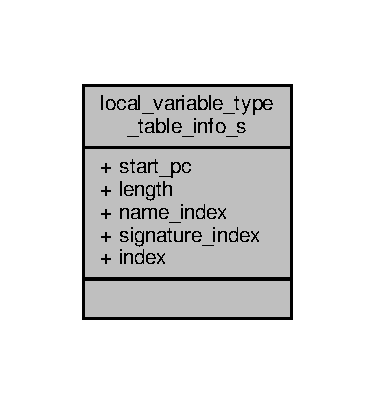
\includegraphics[width=180pt]{structlocal__variable__type__table__info__s__coll__graph}
\end{center}
\end{figure}
\subsection*{Public Attributes}
\begin{DoxyCompactItemize}
\item 
uint16\+\_\+t \hyperlink{structlocal__variable__type__table__info__s_a3c7eafcb1edc9ef0fb4c2f9f48b51847}{start\+\_\+pc}
\item 
uint16\+\_\+t \hyperlink{structlocal__variable__type__table__info__s_a3e805044284c5b623fa5f9309c5e2f1e}{length}
\item 
uint16\+\_\+t \hyperlink{structlocal__variable__type__table__info__s_a1b62a08acc670a50e13ef6f3d655d8a7}{name\+\_\+index}
\item 
uint16\+\_\+t \hyperlink{structlocal__variable__type__table__info__s_a7f6d34460cdca5324e648287fbfc64b3}{signature\+\_\+index}
\item 
uint16\+\_\+t \hyperlink{structlocal__variable__type__table__info__s_ae6348a5edac01de502e54a8dda41394d}{index}
\end{DoxyCompactItemize}


\subsection{Member Data Documentation}
\hypertarget{structlocal__variable__type__table__info__s_ae6348a5edac01de502e54a8dda41394d}{\index{local\+\_\+variable\+\_\+type\+\_\+table\+\_\+info\+\_\+s@{local\+\_\+variable\+\_\+type\+\_\+table\+\_\+info\+\_\+s}!index@{index}}
\index{index@{index}!local\+\_\+variable\+\_\+type\+\_\+table\+\_\+info\+\_\+s@{local\+\_\+variable\+\_\+type\+\_\+table\+\_\+info\+\_\+s}}
\subsubsection[{index}]{\setlength{\rightskip}{0pt plus 5cm}uint16\+\_\+t local\+\_\+variable\+\_\+type\+\_\+table\+\_\+info\+\_\+s\+::index}}\label{structlocal__variable__type__table__info__s_ae6348a5edac01de502e54a8dda41394d}
\hypertarget{structlocal__variable__type__table__info__s_a3e805044284c5b623fa5f9309c5e2f1e}{\index{local\+\_\+variable\+\_\+type\+\_\+table\+\_\+info\+\_\+s@{local\+\_\+variable\+\_\+type\+\_\+table\+\_\+info\+\_\+s}!length@{length}}
\index{length@{length}!local\+\_\+variable\+\_\+type\+\_\+table\+\_\+info\+\_\+s@{local\+\_\+variable\+\_\+type\+\_\+table\+\_\+info\+\_\+s}}
\subsubsection[{length}]{\setlength{\rightskip}{0pt plus 5cm}uint16\+\_\+t local\+\_\+variable\+\_\+type\+\_\+table\+\_\+info\+\_\+s\+::length}}\label{structlocal__variable__type__table__info__s_a3e805044284c5b623fa5f9309c5e2f1e}
\hypertarget{structlocal__variable__type__table__info__s_a1b62a08acc670a50e13ef6f3d655d8a7}{\index{local\+\_\+variable\+\_\+type\+\_\+table\+\_\+info\+\_\+s@{local\+\_\+variable\+\_\+type\+\_\+table\+\_\+info\+\_\+s}!name\+\_\+index@{name\+\_\+index}}
\index{name\+\_\+index@{name\+\_\+index}!local\+\_\+variable\+\_\+type\+\_\+table\+\_\+info\+\_\+s@{local\+\_\+variable\+\_\+type\+\_\+table\+\_\+info\+\_\+s}}
\subsubsection[{name\+\_\+index}]{\setlength{\rightskip}{0pt plus 5cm}uint16\+\_\+t local\+\_\+variable\+\_\+type\+\_\+table\+\_\+info\+\_\+s\+::name\+\_\+index}}\label{structlocal__variable__type__table__info__s_a1b62a08acc670a50e13ef6f3d655d8a7}
\hypertarget{structlocal__variable__type__table__info__s_a7f6d34460cdca5324e648287fbfc64b3}{\index{local\+\_\+variable\+\_\+type\+\_\+table\+\_\+info\+\_\+s@{local\+\_\+variable\+\_\+type\+\_\+table\+\_\+info\+\_\+s}!signature\+\_\+index@{signature\+\_\+index}}
\index{signature\+\_\+index@{signature\+\_\+index}!local\+\_\+variable\+\_\+type\+\_\+table\+\_\+info\+\_\+s@{local\+\_\+variable\+\_\+type\+\_\+table\+\_\+info\+\_\+s}}
\subsubsection[{signature\+\_\+index}]{\setlength{\rightskip}{0pt plus 5cm}uint16\+\_\+t local\+\_\+variable\+\_\+type\+\_\+table\+\_\+info\+\_\+s\+::signature\+\_\+index}}\label{structlocal__variable__type__table__info__s_a7f6d34460cdca5324e648287fbfc64b3}
\hypertarget{structlocal__variable__type__table__info__s_a3c7eafcb1edc9ef0fb4c2f9f48b51847}{\index{local\+\_\+variable\+\_\+type\+\_\+table\+\_\+info\+\_\+s@{local\+\_\+variable\+\_\+type\+\_\+table\+\_\+info\+\_\+s}!start\+\_\+pc@{start\+\_\+pc}}
\index{start\+\_\+pc@{start\+\_\+pc}!local\+\_\+variable\+\_\+type\+\_\+table\+\_\+info\+\_\+s@{local\+\_\+variable\+\_\+type\+\_\+table\+\_\+info\+\_\+s}}
\subsubsection[{start\+\_\+pc}]{\setlength{\rightskip}{0pt plus 5cm}uint16\+\_\+t local\+\_\+variable\+\_\+type\+\_\+table\+\_\+info\+\_\+s\+::start\+\_\+pc}}\label{structlocal__variable__type__table__info__s_a3c7eafcb1edc9ef0fb4c2f9f48b51847}


The documentation for this struct was generated from the following file\+:\begin{DoxyCompactItemize}
\item 
include/\hyperlink{attributes_8hpp}{attributes.\+hpp}\end{DoxyCompactItemize}

\hypertarget{structLocalVariableTable__attribute__s}{\section{Local\+Variable\+Table\+\_\+attribute\+\_\+s Struct Reference}
\label{structLocalVariableTable__attribute__s}\index{Local\+Variable\+Table\+\_\+attribute\+\_\+s@{Local\+Variable\+Table\+\_\+attribute\+\_\+s}}
}


{\ttfamily \#include $<$attributes.\+hpp$>$}



Collaboration diagram for Local\+Variable\+Table\+\_\+attribute\+\_\+s\+:\nopagebreak
\begin{figure}[H]
\begin{center}
\leavevmode
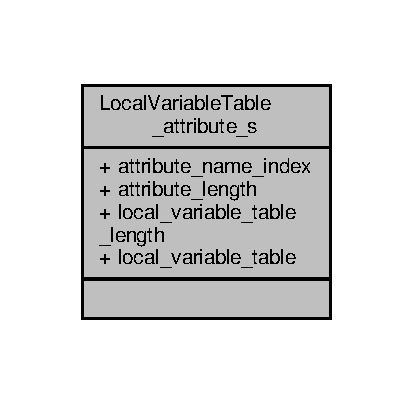
\includegraphics[width=198pt]{structLocalVariableTable__attribute__s__coll__graph}
\end{center}
\end{figure}
\subsection*{Public Attributes}
\begin{DoxyCompactItemize}
\item 
uint16\+\_\+t \hyperlink{structLocalVariableTable__attribute__s_ae575c0e871e3ce914f67b99e05ecae55}{attribute\+\_\+name\+\_\+index}
\item 
uint32\+\_\+t \hyperlink{structLocalVariableTable__attribute__s_a9a3749b259b8912534c5cce4e4582107}{attribute\+\_\+length}
\item 
uint16\+\_\+t \hyperlink{structLocalVariableTable__attribute__s_ac48b8efc7da2e7b280f3c592cc201888}{local\+\_\+variable\+\_\+table\+\_\+length}
\item 
std\+::vector\\*
$<$ \hyperlink{attributes_8hpp_ac0faec3264719598fb702dbf93bbd46f}{local\+\_\+variable\+\_\+table\+\_\+info} $>$ $\ast$ \hyperlink{structLocalVariableTable__attribute__s_a5f3a593bf6cb743eba9590a81822b739}{local\+\_\+variable\+\_\+table}
\end{DoxyCompactItemize}


\subsection{Member Data Documentation}
\hypertarget{structLocalVariableTable__attribute__s_a9a3749b259b8912534c5cce4e4582107}{\index{Local\+Variable\+Table\+\_\+attribute\+\_\+s@{Local\+Variable\+Table\+\_\+attribute\+\_\+s}!attribute\+\_\+length@{attribute\+\_\+length}}
\index{attribute\+\_\+length@{attribute\+\_\+length}!Local\+Variable\+Table\+\_\+attribute\+\_\+s@{Local\+Variable\+Table\+\_\+attribute\+\_\+s}}
\subsubsection[{attribute\+\_\+length}]{\setlength{\rightskip}{0pt plus 5cm}uint32\+\_\+t Local\+Variable\+Table\+\_\+attribute\+\_\+s\+::attribute\+\_\+length}}\label{structLocalVariableTable__attribute__s_a9a3749b259b8912534c5cce4e4582107}
\hypertarget{structLocalVariableTable__attribute__s_ae575c0e871e3ce914f67b99e05ecae55}{\index{Local\+Variable\+Table\+\_\+attribute\+\_\+s@{Local\+Variable\+Table\+\_\+attribute\+\_\+s}!attribute\+\_\+name\+\_\+index@{attribute\+\_\+name\+\_\+index}}
\index{attribute\+\_\+name\+\_\+index@{attribute\+\_\+name\+\_\+index}!Local\+Variable\+Table\+\_\+attribute\+\_\+s@{Local\+Variable\+Table\+\_\+attribute\+\_\+s}}
\subsubsection[{attribute\+\_\+name\+\_\+index}]{\setlength{\rightskip}{0pt plus 5cm}uint16\+\_\+t Local\+Variable\+Table\+\_\+attribute\+\_\+s\+::attribute\+\_\+name\+\_\+index}}\label{structLocalVariableTable__attribute__s_ae575c0e871e3ce914f67b99e05ecae55}
\hypertarget{structLocalVariableTable__attribute__s_a5f3a593bf6cb743eba9590a81822b739}{\index{Local\+Variable\+Table\+\_\+attribute\+\_\+s@{Local\+Variable\+Table\+\_\+attribute\+\_\+s}!local\+\_\+variable\+\_\+table@{local\+\_\+variable\+\_\+table}}
\index{local\+\_\+variable\+\_\+table@{local\+\_\+variable\+\_\+table}!Local\+Variable\+Table\+\_\+attribute\+\_\+s@{Local\+Variable\+Table\+\_\+attribute\+\_\+s}}
\subsubsection[{local\+\_\+variable\+\_\+table}]{\setlength{\rightskip}{0pt plus 5cm}std\+::vector$<${\bf local\+\_\+variable\+\_\+table\+\_\+info}$>$$\ast$ Local\+Variable\+Table\+\_\+attribute\+\_\+s\+::local\+\_\+variable\+\_\+table}}\label{structLocalVariableTable__attribute__s_a5f3a593bf6cb743eba9590a81822b739}
\hypertarget{structLocalVariableTable__attribute__s_ac48b8efc7da2e7b280f3c592cc201888}{\index{Local\+Variable\+Table\+\_\+attribute\+\_\+s@{Local\+Variable\+Table\+\_\+attribute\+\_\+s}!local\+\_\+variable\+\_\+table\+\_\+length@{local\+\_\+variable\+\_\+table\+\_\+length}}
\index{local\+\_\+variable\+\_\+table\+\_\+length@{local\+\_\+variable\+\_\+table\+\_\+length}!Local\+Variable\+Table\+\_\+attribute\+\_\+s@{Local\+Variable\+Table\+\_\+attribute\+\_\+s}}
\subsubsection[{local\+\_\+variable\+\_\+table\+\_\+length}]{\setlength{\rightskip}{0pt plus 5cm}uint16\+\_\+t Local\+Variable\+Table\+\_\+attribute\+\_\+s\+::local\+\_\+variable\+\_\+table\+\_\+length}}\label{structLocalVariableTable__attribute__s_ac48b8efc7da2e7b280f3c592cc201888}


The documentation for this struct was generated from the following file\+:\begin{DoxyCompactItemize}
\item 
include/\hyperlink{attributes_8hpp}{attributes.\+hpp}\end{DoxyCompactItemize}

\hypertarget{structLocalVariableTypeTable__attribute__s}{\section{Local\+Variable\+Type\+Table\+\_\+attribute\+\_\+s Struct Reference}
\label{structLocalVariableTypeTable__attribute__s}\index{Local\+Variable\+Type\+Table\+\_\+attribute\+\_\+s@{Local\+Variable\+Type\+Table\+\_\+attribute\+\_\+s}}
}


{\ttfamily \#include $<$attributes.\+hpp$>$}



Collaboration diagram for Local\+Variable\+Type\+Table\+\_\+attribute\+\_\+s\+:\nopagebreak
\begin{figure}[H]
\begin{center}
\leavevmode
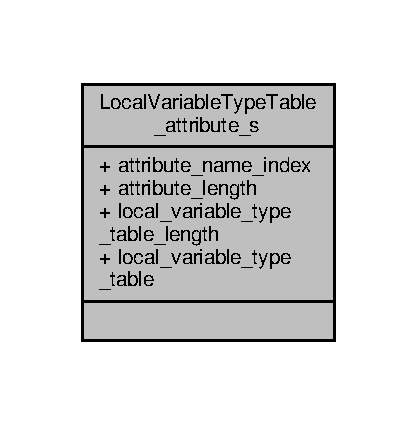
\includegraphics[width=200pt]{structLocalVariableTypeTable__attribute__s__coll__graph}
\end{center}
\end{figure}
\subsection*{Public Attributes}
\begin{DoxyCompactItemize}
\item 
uint16\+\_\+t \hyperlink{structLocalVariableTypeTable__attribute__s_a77c7af17b28fdfe081804f6d7b34a49a}{attribute\+\_\+name\+\_\+index}
\item 
uint32\+\_\+t \hyperlink{structLocalVariableTypeTable__attribute__s_abb4f2b3c349eb2362b044263de18d06e}{attribute\+\_\+length}
\item 
uint16\+\_\+t \hyperlink{structLocalVariableTypeTable__attribute__s_a5f9d25f73fd3f886bc1052974cce379d}{local\+\_\+variable\+\_\+type\+\_\+table\+\_\+length}
\item 
std\+::vector\\*
$<$ \hyperlink{classlocal__variable__type__table__info}{local\+\_\+variable\+\_\+type\+\_\+table\+\_\+info} $>$ $\ast$ \hyperlink{structLocalVariableTypeTable__attribute__s_ad8191d4a435b3c868512e32fce9b613a}{local\+\_\+variable\+\_\+type\+\_\+table}
\end{DoxyCompactItemize}


\subsection{Member Data Documentation}
\hypertarget{structLocalVariableTypeTable__attribute__s_abb4f2b3c349eb2362b044263de18d06e}{\index{Local\+Variable\+Type\+Table\+\_\+attribute\+\_\+s@{Local\+Variable\+Type\+Table\+\_\+attribute\+\_\+s}!attribute\+\_\+length@{attribute\+\_\+length}}
\index{attribute\+\_\+length@{attribute\+\_\+length}!Local\+Variable\+Type\+Table\+\_\+attribute\+\_\+s@{Local\+Variable\+Type\+Table\+\_\+attribute\+\_\+s}}
\subsubsection[{attribute\+\_\+length}]{\setlength{\rightskip}{0pt plus 5cm}uint32\+\_\+t Local\+Variable\+Type\+Table\+\_\+attribute\+\_\+s\+::attribute\+\_\+length}}\label{structLocalVariableTypeTable__attribute__s_abb4f2b3c349eb2362b044263de18d06e}
\hypertarget{structLocalVariableTypeTable__attribute__s_a77c7af17b28fdfe081804f6d7b34a49a}{\index{Local\+Variable\+Type\+Table\+\_\+attribute\+\_\+s@{Local\+Variable\+Type\+Table\+\_\+attribute\+\_\+s}!attribute\+\_\+name\+\_\+index@{attribute\+\_\+name\+\_\+index}}
\index{attribute\+\_\+name\+\_\+index@{attribute\+\_\+name\+\_\+index}!Local\+Variable\+Type\+Table\+\_\+attribute\+\_\+s@{Local\+Variable\+Type\+Table\+\_\+attribute\+\_\+s}}
\subsubsection[{attribute\+\_\+name\+\_\+index}]{\setlength{\rightskip}{0pt plus 5cm}uint16\+\_\+t Local\+Variable\+Type\+Table\+\_\+attribute\+\_\+s\+::attribute\+\_\+name\+\_\+index}}\label{structLocalVariableTypeTable__attribute__s_a77c7af17b28fdfe081804f6d7b34a49a}
\hypertarget{structLocalVariableTypeTable__attribute__s_ad8191d4a435b3c868512e32fce9b613a}{\index{Local\+Variable\+Type\+Table\+\_\+attribute\+\_\+s@{Local\+Variable\+Type\+Table\+\_\+attribute\+\_\+s}!local\+\_\+variable\+\_\+type\+\_\+table@{local\+\_\+variable\+\_\+type\+\_\+table}}
\index{local\+\_\+variable\+\_\+type\+\_\+table@{local\+\_\+variable\+\_\+type\+\_\+table}!Local\+Variable\+Type\+Table\+\_\+attribute\+\_\+s@{Local\+Variable\+Type\+Table\+\_\+attribute\+\_\+s}}
\subsubsection[{local\+\_\+variable\+\_\+type\+\_\+table}]{\setlength{\rightskip}{0pt plus 5cm}std\+::vector$<${\bf local\+\_\+variable\+\_\+type\+\_\+table\+\_\+info}$>$$\ast$ Local\+Variable\+Type\+Table\+\_\+attribute\+\_\+s\+::local\+\_\+variable\+\_\+type\+\_\+table}}\label{structLocalVariableTypeTable__attribute__s_ad8191d4a435b3c868512e32fce9b613a}
\hypertarget{structLocalVariableTypeTable__attribute__s_a5f9d25f73fd3f886bc1052974cce379d}{\index{Local\+Variable\+Type\+Table\+\_\+attribute\+\_\+s@{Local\+Variable\+Type\+Table\+\_\+attribute\+\_\+s}!local\+\_\+variable\+\_\+type\+\_\+table\+\_\+length@{local\+\_\+variable\+\_\+type\+\_\+table\+\_\+length}}
\index{local\+\_\+variable\+\_\+type\+\_\+table\+\_\+length@{local\+\_\+variable\+\_\+type\+\_\+table\+\_\+length}!Local\+Variable\+Type\+Table\+\_\+attribute\+\_\+s@{Local\+Variable\+Type\+Table\+\_\+attribute\+\_\+s}}
\subsubsection[{local\+\_\+variable\+\_\+type\+\_\+table\+\_\+length}]{\setlength{\rightskip}{0pt plus 5cm}uint16\+\_\+t Local\+Variable\+Type\+Table\+\_\+attribute\+\_\+s\+::local\+\_\+variable\+\_\+type\+\_\+table\+\_\+length}}\label{structLocalVariableTypeTable__attribute__s_a5f9d25f73fd3f886bc1052974cce379d}


The documentation for this struct was generated from the following file\+:\begin{DoxyCompactItemize}
\item 
include/\hyperlink{attributes_8hpp}{attributes.\+hpp}\end{DoxyCompactItemize}

\hypertarget{structmethod__info__s}{\section{method\+\_\+info\+\_\+s Struct Reference}
\label{structmethod__info__s}\index{method\+\_\+info\+\_\+s@{method\+\_\+info\+\_\+s}}
}


{\ttfamily \#include $<$structs.\+hpp$>$}



Collaboration diagram for method\+\_\+info\+\_\+s\+:\nopagebreak
\begin{figure}[H]
\begin{center}
\leavevmode
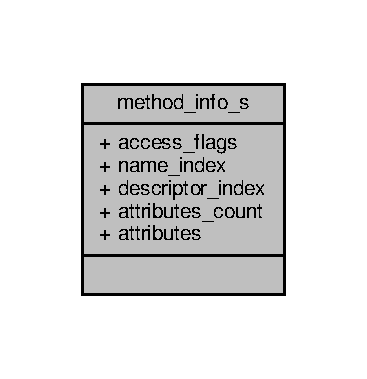
\includegraphics[width=176pt]{structmethod__info__s__coll__graph}
\end{center}
\end{figure}
\subsection*{Public Attributes}
\begin{DoxyCompactItemize}
\item 
uint16\+\_\+t \hyperlink{structmethod__info__s_a062a031a987939214bf617101bce7435}{access\+\_\+flags}
\item 
uint16\+\_\+t \hyperlink{structmethod__info__s_ae7934a7245dbcbb518002309acbb53ae}{name\+\_\+index}
\item 
uint16\+\_\+t \hyperlink{structmethod__info__s_af93c8318d7968679bf177a79ca5df51b}{descriptor\+\_\+index}
\item 
uint16\+\_\+t \hyperlink{structmethod__info__s_afbbdab1523d8260e88ca3b0e09ad579d}{attributes\+\_\+count}
\item 
std\+::vector$<$ \hyperlink{attributes_8hpp_a7af51299ff517acce960ac87c9db9899}{attribute\+\_\+info} $>$ \hyperlink{structmethod__info__s_a4e4f4472bdd775cda7fdc50797defe66}{attributes}
\end{DoxyCompactItemize}


\subsection{Member Data Documentation}
\hypertarget{structmethod__info__s_a062a031a987939214bf617101bce7435}{\index{method\+\_\+info\+\_\+s@{method\+\_\+info\+\_\+s}!access\+\_\+flags@{access\+\_\+flags}}
\index{access\+\_\+flags@{access\+\_\+flags}!method\+\_\+info\+\_\+s@{method\+\_\+info\+\_\+s}}
\subsubsection[{access\+\_\+flags}]{\setlength{\rightskip}{0pt plus 5cm}uint16\+\_\+t method\+\_\+info\+\_\+s\+::access\+\_\+flags}}\label{structmethod__info__s_a062a031a987939214bf617101bce7435}
\hypertarget{structmethod__info__s_a4e4f4472bdd775cda7fdc50797defe66}{\index{method\+\_\+info\+\_\+s@{method\+\_\+info\+\_\+s}!attributes@{attributes}}
\index{attributes@{attributes}!method\+\_\+info\+\_\+s@{method\+\_\+info\+\_\+s}}
\subsubsection[{attributes}]{\setlength{\rightskip}{0pt plus 5cm}std\+::vector$<${\bf attribute\+\_\+info}$>$ method\+\_\+info\+\_\+s\+::attributes}}\label{structmethod__info__s_a4e4f4472bdd775cda7fdc50797defe66}
\hypertarget{structmethod__info__s_afbbdab1523d8260e88ca3b0e09ad579d}{\index{method\+\_\+info\+\_\+s@{method\+\_\+info\+\_\+s}!attributes\+\_\+count@{attributes\+\_\+count}}
\index{attributes\+\_\+count@{attributes\+\_\+count}!method\+\_\+info\+\_\+s@{method\+\_\+info\+\_\+s}}
\subsubsection[{attributes\+\_\+count}]{\setlength{\rightskip}{0pt plus 5cm}uint16\+\_\+t method\+\_\+info\+\_\+s\+::attributes\+\_\+count}}\label{structmethod__info__s_afbbdab1523d8260e88ca3b0e09ad579d}
\hypertarget{structmethod__info__s_af93c8318d7968679bf177a79ca5df51b}{\index{method\+\_\+info\+\_\+s@{method\+\_\+info\+\_\+s}!descriptor\+\_\+index@{descriptor\+\_\+index}}
\index{descriptor\+\_\+index@{descriptor\+\_\+index}!method\+\_\+info\+\_\+s@{method\+\_\+info\+\_\+s}}
\subsubsection[{descriptor\+\_\+index}]{\setlength{\rightskip}{0pt plus 5cm}uint16\+\_\+t method\+\_\+info\+\_\+s\+::descriptor\+\_\+index}}\label{structmethod__info__s_af93c8318d7968679bf177a79ca5df51b}
\hypertarget{structmethod__info__s_ae7934a7245dbcbb518002309acbb53ae}{\index{method\+\_\+info\+\_\+s@{method\+\_\+info\+\_\+s}!name\+\_\+index@{name\+\_\+index}}
\index{name\+\_\+index@{name\+\_\+index}!method\+\_\+info\+\_\+s@{method\+\_\+info\+\_\+s}}
\subsubsection[{name\+\_\+index}]{\setlength{\rightskip}{0pt plus 5cm}uint16\+\_\+t method\+\_\+info\+\_\+s\+::name\+\_\+index}}\label{structmethod__info__s_ae7934a7245dbcbb518002309acbb53ae}


The documentation for this struct was generated from the following file\+:\begin{DoxyCompactItemize}
\item 
include/\hyperlink{structs_8hpp}{structs.\+hpp}\end{DoxyCompactItemize}

\hypertarget{structoperand__s}{\section{operand\+\_\+s Struct Reference}
\label{structoperand__s}\index{operand\+\_\+s@{operand\+\_\+s}}
}


{\ttfamily \#include $<$frame.\+hpp$>$}



Collaboration diagram for operand\+\_\+s\+:\nopagebreak
\begin{figure}[H]
\begin{center}
\leavevmode
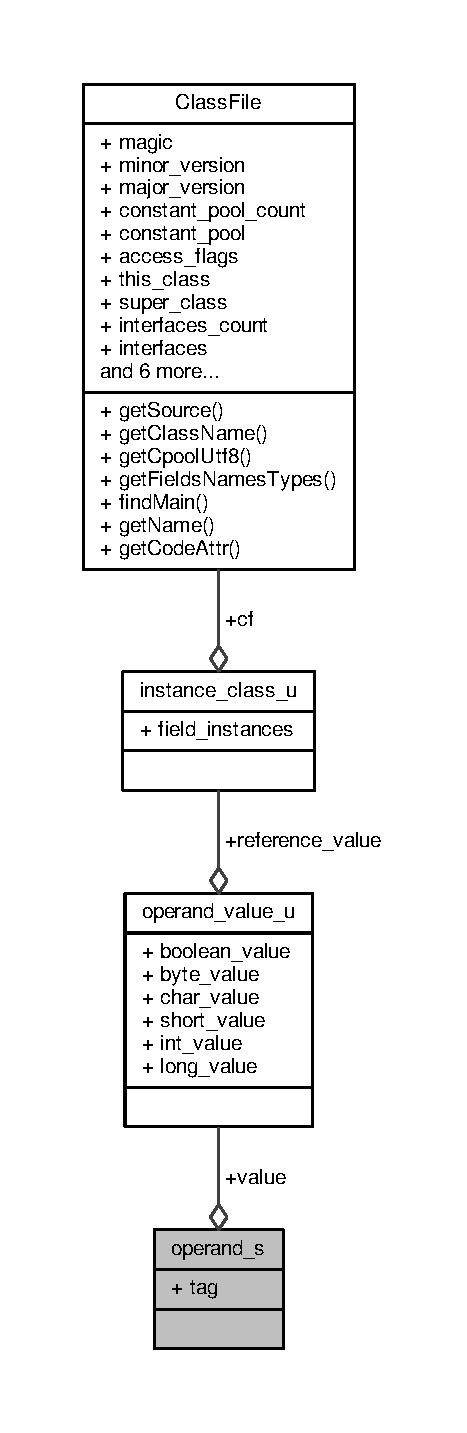
\includegraphics[height=550pt]{structoperand__s__coll__graph}
\end{center}
\end{figure}
\subsection*{Public Attributes}
\begin{DoxyCompactItemize}
\item 
uint8\+\_\+t \hyperlink{structoperand__s_a3096a61fdc761a5231b863b2945165bb}{tag}
\item 
\hyperlink{frame_8hpp_a1082aacc4b1471d93e3277f0d0209e72}{operand\+\_\+value} \hyperlink{structoperand__s_ae5e9c83467419221b9bc57dd8dff5ad6}{value}
\end{DoxyCompactItemize}


\subsection{Member Data Documentation}
\hypertarget{structoperand__s_a3096a61fdc761a5231b863b2945165bb}{\index{operand\+\_\+s@{operand\+\_\+s}!tag@{tag}}
\index{tag@{tag}!operand\+\_\+s@{operand\+\_\+s}}
\subsubsection[{tag}]{\setlength{\rightskip}{0pt plus 5cm}uint8\+\_\+t operand\+\_\+s\+::tag}}\label{structoperand__s_a3096a61fdc761a5231b863b2945165bb}
\hypertarget{structoperand__s_ae5e9c83467419221b9bc57dd8dff5ad6}{\index{operand\+\_\+s@{operand\+\_\+s}!value@{value}}
\index{value@{value}!operand\+\_\+s@{operand\+\_\+s}}
\subsubsection[{value}]{\setlength{\rightskip}{0pt plus 5cm}{\bf operand\+\_\+value} operand\+\_\+s\+::value}}\label{structoperand__s_ae5e9c83467419221b9bc57dd8dff5ad6}


The documentation for this struct was generated from the following file\+:\begin{DoxyCompactItemize}
\item 
include/\hyperlink{frame_8hpp}{frame.\+hpp}\end{DoxyCompactItemize}

\hypertarget{unionoperand__value__u}{\section{operand\+\_\+value\+\_\+u Union Reference}
\label{unionoperand__value__u}\index{operand\+\_\+value\+\_\+u@{operand\+\_\+value\+\_\+u}}
}


{\ttfamily \#include $<$frame.\+hpp$>$}



Collaboration diagram for operand\+\_\+value\+\_\+u\+:\nopagebreak
\begin{figure}[H]
\begin{center}
\leavevmode
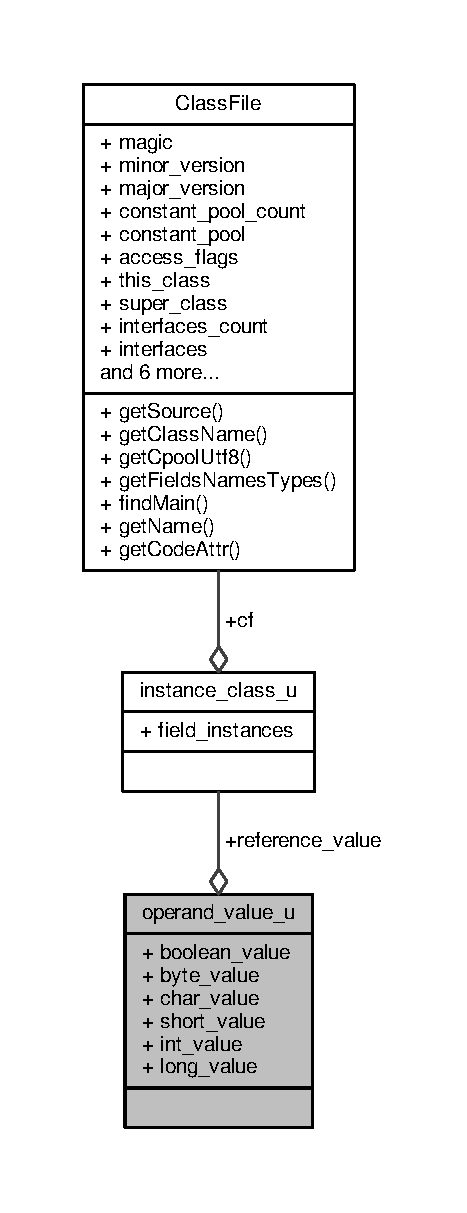
\includegraphics[height=550pt]{unionoperand__value__u__coll__graph}
\end{center}
\end{figure}
\subsection*{Public Attributes}
\begin{DoxyCompactItemize}
\item 
bool \hyperlink{unionoperand__value__u_ae24e297c8249a0c4191357646a8e3769}{boolean\+\_\+value}
\item 
uint8\+\_\+t \hyperlink{unionoperand__value__u_a21b4bc4455c8e80d6044a92048e25fc8}{byte\+\_\+value}
\item 
uint8\+\_\+t \hyperlink{unionoperand__value__u_aa32123b56a07f688c63369422f3bf028}{char\+\_\+value}
\item 
int16\+\_\+t \hyperlink{unionoperand__value__u_aa25b00a9b4e1a83eb0c640c50b055bc9}{short\+\_\+value}
\item 
int32\+\_\+t \hyperlink{unionoperand__value__u_a2cf0c99efed244d66e915b663897d147}{int\+\_\+value}
\item 
int64\+\_\+t \hyperlink{unionoperand__value__u_a867f9ef828309d9781b887d12f606199}{long\+\_\+value}
\item 
\hyperlink{heap_8hpp_a10a6b663306bb9ebfa5959ab91c79eda}{Instance\+Class} $\ast$ \hyperlink{unionoperand__value__u_af760b5c7bc708eb1d4ec87a9489b57ef}{reference\+\_\+value}
\end{DoxyCompactItemize}


\subsection{Member Data Documentation}
\hypertarget{unionoperand__value__u_ae24e297c8249a0c4191357646a8e3769}{\index{operand\+\_\+value\+\_\+u@{operand\+\_\+value\+\_\+u}!boolean\+\_\+value@{boolean\+\_\+value}}
\index{boolean\+\_\+value@{boolean\+\_\+value}!operand\+\_\+value\+\_\+u@{operand\+\_\+value\+\_\+u}}
\subsubsection[{boolean\+\_\+value}]{\setlength{\rightskip}{0pt plus 5cm}bool operand\+\_\+value\+\_\+u\+::boolean\+\_\+value}}\label{unionoperand__value__u_ae24e297c8249a0c4191357646a8e3769}
\hypertarget{unionoperand__value__u_a21b4bc4455c8e80d6044a92048e25fc8}{\index{operand\+\_\+value\+\_\+u@{operand\+\_\+value\+\_\+u}!byte\+\_\+value@{byte\+\_\+value}}
\index{byte\+\_\+value@{byte\+\_\+value}!operand\+\_\+value\+\_\+u@{operand\+\_\+value\+\_\+u}}
\subsubsection[{byte\+\_\+value}]{\setlength{\rightskip}{0pt plus 5cm}uint8\+\_\+t operand\+\_\+value\+\_\+u\+::byte\+\_\+value}}\label{unionoperand__value__u_a21b4bc4455c8e80d6044a92048e25fc8}
\hypertarget{unionoperand__value__u_aa32123b56a07f688c63369422f3bf028}{\index{operand\+\_\+value\+\_\+u@{operand\+\_\+value\+\_\+u}!char\+\_\+value@{char\+\_\+value}}
\index{char\+\_\+value@{char\+\_\+value}!operand\+\_\+value\+\_\+u@{operand\+\_\+value\+\_\+u}}
\subsubsection[{char\+\_\+value}]{\setlength{\rightskip}{0pt plus 5cm}uint8\+\_\+t operand\+\_\+value\+\_\+u\+::char\+\_\+value}}\label{unionoperand__value__u_aa32123b56a07f688c63369422f3bf028}
\hypertarget{unionoperand__value__u_a2cf0c99efed244d66e915b663897d147}{\index{operand\+\_\+value\+\_\+u@{operand\+\_\+value\+\_\+u}!int\+\_\+value@{int\+\_\+value}}
\index{int\+\_\+value@{int\+\_\+value}!operand\+\_\+value\+\_\+u@{operand\+\_\+value\+\_\+u}}
\subsubsection[{int\+\_\+value}]{\setlength{\rightskip}{0pt plus 5cm}int32\+\_\+t operand\+\_\+value\+\_\+u\+::int\+\_\+value}}\label{unionoperand__value__u_a2cf0c99efed244d66e915b663897d147}
\hypertarget{unionoperand__value__u_a867f9ef828309d9781b887d12f606199}{\index{operand\+\_\+value\+\_\+u@{operand\+\_\+value\+\_\+u}!long\+\_\+value@{long\+\_\+value}}
\index{long\+\_\+value@{long\+\_\+value}!operand\+\_\+value\+\_\+u@{operand\+\_\+value\+\_\+u}}
\subsubsection[{long\+\_\+value}]{\setlength{\rightskip}{0pt plus 5cm}int64\+\_\+t operand\+\_\+value\+\_\+u\+::long\+\_\+value}}\label{unionoperand__value__u_a867f9ef828309d9781b887d12f606199}
\hypertarget{unionoperand__value__u_af760b5c7bc708eb1d4ec87a9489b57ef}{\index{operand\+\_\+value\+\_\+u@{operand\+\_\+value\+\_\+u}!reference\+\_\+value@{reference\+\_\+value}}
\index{reference\+\_\+value@{reference\+\_\+value}!operand\+\_\+value\+\_\+u@{operand\+\_\+value\+\_\+u}}
\subsubsection[{reference\+\_\+value}]{\setlength{\rightskip}{0pt plus 5cm}{\bf Instance\+Class}$\ast$ operand\+\_\+value\+\_\+u\+::reference\+\_\+value}}\label{unionoperand__value__u_af760b5c7bc708eb1d4ec87a9489b57ef}
\hypertarget{unionoperand__value__u_aa25b00a9b4e1a83eb0c640c50b055bc9}{\index{operand\+\_\+value\+\_\+u@{operand\+\_\+value\+\_\+u}!short\+\_\+value@{short\+\_\+value}}
\index{short\+\_\+value@{short\+\_\+value}!operand\+\_\+value\+\_\+u@{operand\+\_\+value\+\_\+u}}
\subsubsection[{short\+\_\+value}]{\setlength{\rightskip}{0pt plus 5cm}int16\+\_\+t operand\+\_\+value\+\_\+u\+::short\+\_\+value}}\label{unionoperand__value__u_aa25b00a9b4e1a83eb0c640c50b055bc9}


The documentation for this union was generated from the following file\+:\begin{DoxyCompactItemize}
\item 
include/\hyperlink{frame_8hpp}{frame.\+hpp}\end{DoxyCompactItemize}

\hypertarget{structSignature__attribute__s}{\section{Signature\+\_\+attribute\+\_\+s Struct Reference}
\label{structSignature__attribute__s}\index{Signature\+\_\+attribute\+\_\+s@{Signature\+\_\+attribute\+\_\+s}}
}


{\ttfamily \#include $<$attributes.\+hpp$>$}



Collaboration diagram for Signature\+\_\+attribute\+\_\+s\+:\nopagebreak
\begin{figure}[H]
\begin{center}
\leavevmode
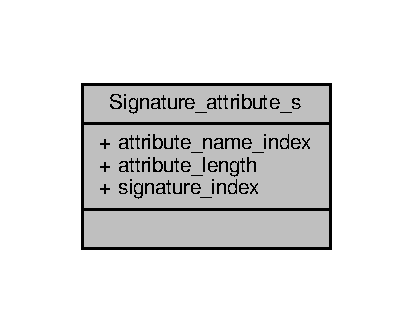
\includegraphics[width=198pt]{structSignature__attribute__s__coll__graph}
\end{center}
\end{figure}
\subsection*{Public Attributes}
\begin{DoxyCompactItemize}
\item 
uint16\+\_\+t \hyperlink{structSignature__attribute__s_a6c63cbbb5e2570691c9ae328440ae58f}{attribute\+\_\+name\+\_\+index}
\item 
uint32\+\_\+t \hyperlink{structSignature__attribute__s_a4a57dffe751f28ffe046dfdefe4a46fd}{attribute\+\_\+length}
\item 
uint16\+\_\+t \hyperlink{structSignature__attribute__s_a8c7f7f5f3002f25e5bfa1b637000433d}{signature\+\_\+index}
\end{DoxyCompactItemize}


\subsection{Member Data Documentation}
\hypertarget{structSignature__attribute__s_a4a57dffe751f28ffe046dfdefe4a46fd}{\index{Signature\+\_\+attribute\+\_\+s@{Signature\+\_\+attribute\+\_\+s}!attribute\+\_\+length@{attribute\+\_\+length}}
\index{attribute\+\_\+length@{attribute\+\_\+length}!Signature\+\_\+attribute\+\_\+s@{Signature\+\_\+attribute\+\_\+s}}
\subsubsection[{attribute\+\_\+length}]{\setlength{\rightskip}{0pt plus 5cm}uint32\+\_\+t Signature\+\_\+attribute\+\_\+s\+::attribute\+\_\+length}}\label{structSignature__attribute__s_a4a57dffe751f28ffe046dfdefe4a46fd}
\hypertarget{structSignature__attribute__s_a6c63cbbb5e2570691c9ae328440ae58f}{\index{Signature\+\_\+attribute\+\_\+s@{Signature\+\_\+attribute\+\_\+s}!attribute\+\_\+name\+\_\+index@{attribute\+\_\+name\+\_\+index}}
\index{attribute\+\_\+name\+\_\+index@{attribute\+\_\+name\+\_\+index}!Signature\+\_\+attribute\+\_\+s@{Signature\+\_\+attribute\+\_\+s}}
\subsubsection[{attribute\+\_\+name\+\_\+index}]{\setlength{\rightskip}{0pt plus 5cm}uint16\+\_\+t Signature\+\_\+attribute\+\_\+s\+::attribute\+\_\+name\+\_\+index}}\label{structSignature__attribute__s_a6c63cbbb5e2570691c9ae328440ae58f}
\hypertarget{structSignature__attribute__s_a8c7f7f5f3002f25e5bfa1b637000433d}{\index{Signature\+\_\+attribute\+\_\+s@{Signature\+\_\+attribute\+\_\+s}!signature\+\_\+index@{signature\+\_\+index}}
\index{signature\+\_\+index@{signature\+\_\+index}!Signature\+\_\+attribute\+\_\+s@{Signature\+\_\+attribute\+\_\+s}}
\subsubsection[{signature\+\_\+index}]{\setlength{\rightskip}{0pt plus 5cm}uint16\+\_\+t Signature\+\_\+attribute\+\_\+s\+::signature\+\_\+index}}\label{structSignature__attribute__s_a8c7f7f5f3002f25e5bfa1b637000433d}


The documentation for this struct was generated from the following file\+:\begin{DoxyCompactItemize}
\item 
include/\hyperlink{attributes_8hpp}{attributes.\+hpp}\end{DoxyCompactItemize}

\hypertarget{structSourceFile__attribute__s}{\section{Source\+File\+\_\+attribute\+\_\+s Struct Reference}
\label{structSourceFile__attribute__s}\index{Source\+File\+\_\+attribute\+\_\+s@{Source\+File\+\_\+attribute\+\_\+s}}
}


{\ttfamily \#include $<$attributes.\+hpp$>$}



Collaboration diagram for Source\+File\+\_\+attribute\+\_\+s\+:\nopagebreak
\begin{figure}[H]
\begin{center}
\leavevmode
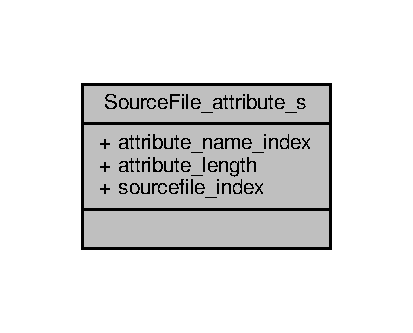
\includegraphics[width=198pt]{structSourceFile__attribute__s__coll__graph}
\end{center}
\end{figure}
\subsection*{Public Attributes}
\begin{DoxyCompactItemize}
\item 
uint16\+\_\+t \hyperlink{structSourceFile__attribute__s_af373e87d77acccb3b69b491062fa12ea}{attribute\+\_\+name\+\_\+index}
\item 
uint32\+\_\+t \hyperlink{structSourceFile__attribute__s_a3aad253479910514937e30e6874c37cd}{attribute\+\_\+length}
\item 
uint16\+\_\+t \hyperlink{structSourceFile__attribute__s_a58a666cf2e0ffd0557d6edc270bf195f}{sourcefile\+\_\+index}
\end{DoxyCompactItemize}


\subsection{Member Data Documentation}
\hypertarget{structSourceFile__attribute__s_a3aad253479910514937e30e6874c37cd}{\index{Source\+File\+\_\+attribute\+\_\+s@{Source\+File\+\_\+attribute\+\_\+s}!attribute\+\_\+length@{attribute\+\_\+length}}
\index{attribute\+\_\+length@{attribute\+\_\+length}!Source\+File\+\_\+attribute\+\_\+s@{Source\+File\+\_\+attribute\+\_\+s}}
\subsubsection[{attribute\+\_\+length}]{\setlength{\rightskip}{0pt plus 5cm}uint32\+\_\+t Source\+File\+\_\+attribute\+\_\+s\+::attribute\+\_\+length}}\label{structSourceFile__attribute__s_a3aad253479910514937e30e6874c37cd}
\hypertarget{structSourceFile__attribute__s_af373e87d77acccb3b69b491062fa12ea}{\index{Source\+File\+\_\+attribute\+\_\+s@{Source\+File\+\_\+attribute\+\_\+s}!attribute\+\_\+name\+\_\+index@{attribute\+\_\+name\+\_\+index}}
\index{attribute\+\_\+name\+\_\+index@{attribute\+\_\+name\+\_\+index}!Source\+File\+\_\+attribute\+\_\+s@{Source\+File\+\_\+attribute\+\_\+s}}
\subsubsection[{attribute\+\_\+name\+\_\+index}]{\setlength{\rightskip}{0pt plus 5cm}uint16\+\_\+t Source\+File\+\_\+attribute\+\_\+s\+::attribute\+\_\+name\+\_\+index}}\label{structSourceFile__attribute__s_af373e87d77acccb3b69b491062fa12ea}
\hypertarget{structSourceFile__attribute__s_a58a666cf2e0ffd0557d6edc270bf195f}{\index{Source\+File\+\_\+attribute\+\_\+s@{Source\+File\+\_\+attribute\+\_\+s}!sourcefile\+\_\+index@{sourcefile\+\_\+index}}
\index{sourcefile\+\_\+index@{sourcefile\+\_\+index}!Source\+File\+\_\+attribute\+\_\+s@{Source\+File\+\_\+attribute\+\_\+s}}
\subsubsection[{sourcefile\+\_\+index}]{\setlength{\rightskip}{0pt plus 5cm}uint16\+\_\+t Source\+File\+\_\+attribute\+\_\+s\+::sourcefile\+\_\+index}}\label{structSourceFile__attribute__s_a58a666cf2e0ffd0557d6edc270bf195f}


The documentation for this struct was generated from the following file\+:\begin{DoxyCompactItemize}
\item 
include/\hyperlink{attributes_8hpp}{attributes.\+hpp}\end{DoxyCompactItemize}

\hypertarget{structSynthetic__attribute__s}{\section{Synthetic\+\_\+attribute\+\_\+s Struct Reference}
\label{structSynthetic__attribute__s}\index{Synthetic\+\_\+attribute\+\_\+s@{Synthetic\+\_\+attribute\+\_\+s}}
}


{\ttfamily \#include $<$attributes.\+hpp$>$}



Collaboration diagram for Synthetic\+\_\+attribute\+\_\+s\+:\nopagebreak
\begin{figure}[H]
\begin{center}
\leavevmode
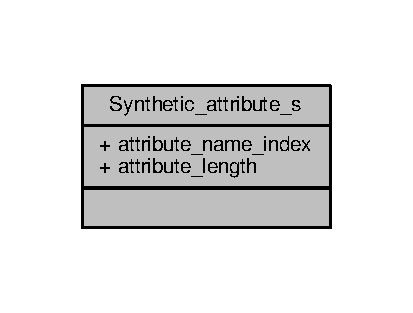
\includegraphics[width=198pt]{structSynthetic__attribute__s__coll__graph}
\end{center}
\end{figure}
\subsection*{Public Attributes}
\begin{DoxyCompactItemize}
\item 
uint16\+\_\+t \hyperlink{structSynthetic__attribute__s_a40701978ef09290bcaa9793503312706}{attribute\+\_\+name\+\_\+index}
\item 
uint32\+\_\+t \hyperlink{structSynthetic__attribute__s_a3c8e6a2024b6646ced85a7414040b6f6}{attribute\+\_\+length}
\end{DoxyCompactItemize}


\subsection{Member Data Documentation}
\hypertarget{structSynthetic__attribute__s_a3c8e6a2024b6646ced85a7414040b6f6}{\index{Synthetic\+\_\+attribute\+\_\+s@{Synthetic\+\_\+attribute\+\_\+s}!attribute\+\_\+length@{attribute\+\_\+length}}
\index{attribute\+\_\+length@{attribute\+\_\+length}!Synthetic\+\_\+attribute\+\_\+s@{Synthetic\+\_\+attribute\+\_\+s}}
\subsubsection[{attribute\+\_\+length}]{\setlength{\rightskip}{0pt plus 5cm}uint32\+\_\+t Synthetic\+\_\+attribute\+\_\+s\+::attribute\+\_\+length}}\label{structSynthetic__attribute__s_a3c8e6a2024b6646ced85a7414040b6f6}
\hypertarget{structSynthetic__attribute__s_a40701978ef09290bcaa9793503312706}{\index{Synthetic\+\_\+attribute\+\_\+s@{Synthetic\+\_\+attribute\+\_\+s}!attribute\+\_\+name\+\_\+index@{attribute\+\_\+name\+\_\+index}}
\index{attribute\+\_\+name\+\_\+index@{attribute\+\_\+name\+\_\+index}!Synthetic\+\_\+attribute\+\_\+s@{Synthetic\+\_\+attribute\+\_\+s}}
\subsubsection[{attribute\+\_\+name\+\_\+index}]{\setlength{\rightskip}{0pt plus 5cm}uint16\+\_\+t Synthetic\+\_\+attribute\+\_\+s\+::attribute\+\_\+name\+\_\+index}}\label{structSynthetic__attribute__s_a40701978ef09290bcaa9793503312706}


The documentation for this struct was generated from the following file\+:\begin{DoxyCompactItemize}
\item 
include/\hyperlink{attributes_8hpp}{attributes.\+hpp}\end{DoxyCompactItemize}

\hypertarget{structtions__attribute__s}{\section{tions\+\_\+attribute\+\_\+s Struct Reference}
\label{structtions__attribute__s}\index{tions\+\_\+attribute\+\_\+s@{tions\+\_\+attribute\+\_\+s}}
}


{\ttfamily \#include $<$attributes.\+hpp$>$}



Collaboration diagram for tions\+\_\+attribute\+\_\+s\+:\nopagebreak
\begin{figure}[H]
\begin{center}
\leavevmode
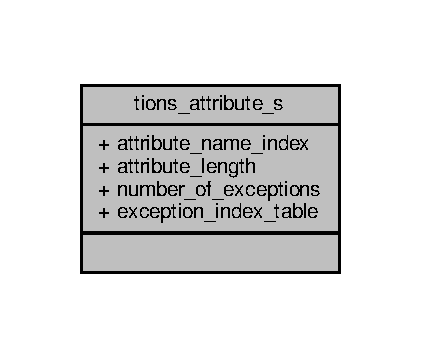
\includegraphics[width=202pt]{structtions__attribute__s__coll__graph}
\end{center}
\end{figure}
\subsection*{Public Attributes}
\begin{DoxyCompactItemize}
\item 
uint16\+\_\+t \hyperlink{structtions__attribute__s_a9b8db8dc3f0a915e0ea293b4a02aced5}{attribute\+\_\+name\+\_\+index}
\item 
uint32\+\_\+t \hyperlink{structtions__attribute__s_ab0b8c06d504e802ce01a0943bbd9bf10}{attribute\+\_\+length}
\item 
uint16\+\_\+t \hyperlink{structtions__attribute__s_a742ecd8b40b51ba831806ec14299c053}{number\+\_\+of\+\_\+exceptions}
\item 
std\+::vector$<$ uint16\+\_\+t $>$ $\ast$ \hyperlink{structtions__attribute__s_affcf7f1a4bad06d919af96858d87a9e6}{exception\+\_\+index\+\_\+table}
\end{DoxyCompactItemize}


\subsection{Member Data Documentation}
\hypertarget{structtions__attribute__s_ab0b8c06d504e802ce01a0943bbd9bf10}{\index{tions\+\_\+attribute\+\_\+s@{tions\+\_\+attribute\+\_\+s}!attribute\+\_\+length@{attribute\+\_\+length}}
\index{attribute\+\_\+length@{attribute\+\_\+length}!tions\+\_\+attribute\+\_\+s@{tions\+\_\+attribute\+\_\+s}}
\subsubsection[{attribute\+\_\+length}]{\setlength{\rightskip}{0pt plus 5cm}uint32\+\_\+t tions\+\_\+attribute\+\_\+s\+::attribute\+\_\+length}}\label{structtions__attribute__s_ab0b8c06d504e802ce01a0943bbd9bf10}
\hypertarget{structtions__attribute__s_a9b8db8dc3f0a915e0ea293b4a02aced5}{\index{tions\+\_\+attribute\+\_\+s@{tions\+\_\+attribute\+\_\+s}!attribute\+\_\+name\+\_\+index@{attribute\+\_\+name\+\_\+index}}
\index{attribute\+\_\+name\+\_\+index@{attribute\+\_\+name\+\_\+index}!tions\+\_\+attribute\+\_\+s@{tions\+\_\+attribute\+\_\+s}}
\subsubsection[{attribute\+\_\+name\+\_\+index}]{\setlength{\rightskip}{0pt plus 5cm}uint16\+\_\+t tions\+\_\+attribute\+\_\+s\+::attribute\+\_\+name\+\_\+index}}\label{structtions__attribute__s_a9b8db8dc3f0a915e0ea293b4a02aced5}
\hypertarget{structtions__attribute__s_affcf7f1a4bad06d919af96858d87a9e6}{\index{tions\+\_\+attribute\+\_\+s@{tions\+\_\+attribute\+\_\+s}!exception\+\_\+index\+\_\+table@{exception\+\_\+index\+\_\+table}}
\index{exception\+\_\+index\+\_\+table@{exception\+\_\+index\+\_\+table}!tions\+\_\+attribute\+\_\+s@{tions\+\_\+attribute\+\_\+s}}
\subsubsection[{exception\+\_\+index\+\_\+table}]{\setlength{\rightskip}{0pt plus 5cm}std\+::vector$<$uint16\+\_\+t$>$$\ast$ tions\+\_\+attribute\+\_\+s\+::exception\+\_\+index\+\_\+table}}\label{structtions__attribute__s_affcf7f1a4bad06d919af96858d87a9e6}
\hypertarget{structtions__attribute__s_a742ecd8b40b51ba831806ec14299c053}{\index{tions\+\_\+attribute\+\_\+s@{tions\+\_\+attribute\+\_\+s}!number\+\_\+of\+\_\+exceptions@{number\+\_\+of\+\_\+exceptions}}
\index{number\+\_\+of\+\_\+exceptions@{number\+\_\+of\+\_\+exceptions}!tions\+\_\+attribute\+\_\+s@{tions\+\_\+attribute\+\_\+s}}
\subsubsection[{number\+\_\+of\+\_\+exceptions}]{\setlength{\rightskip}{0pt plus 5cm}uint16\+\_\+t tions\+\_\+attribute\+\_\+s\+::number\+\_\+of\+\_\+exceptions}}\label{structtions__attribute__s_a742ecd8b40b51ba831806ec14299c053}


The documentation for this struct was generated from the following file\+:\begin{DoxyCompactItemize}
\item 
include/\hyperlink{attributes_8hpp}{attributes.\+hpp}\end{DoxyCompactItemize}

\hypertarget{uniontype__s}{\section{type\+\_\+s Union Reference}
\label{uniontype__s}\index{type\+\_\+s@{type\+\_\+s}}
}


{\ttfamily \#include $<$heap.\+hpp$>$}



Collaboration diagram for type\+\_\+s\+:\nopagebreak
\begin{figure}[H]
\begin{center}
\leavevmode
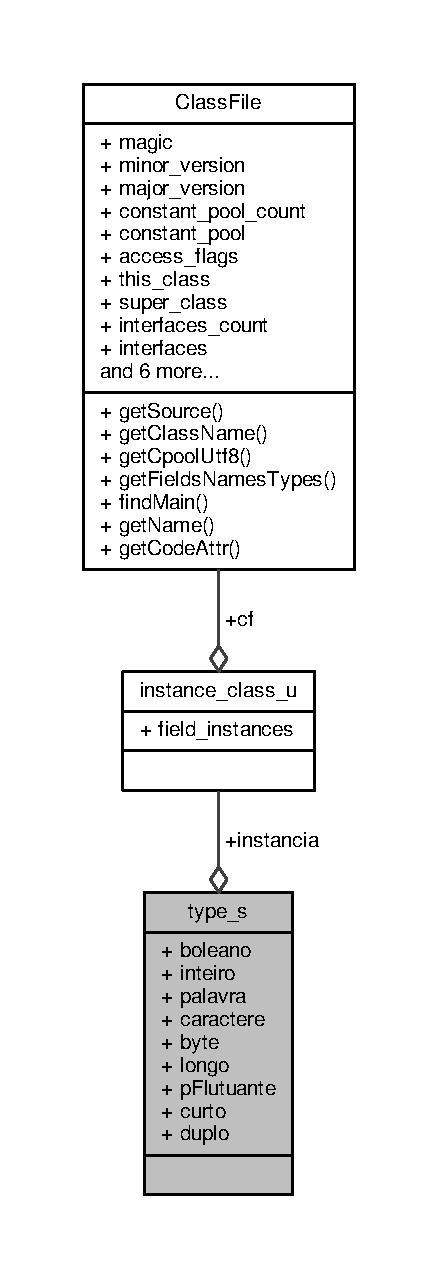
\includegraphics[height=550pt]{uniontype__s__coll__graph}
\end{center}
\end{figure}
\subsection*{Public Attributes}
\begin{DoxyCompactItemize}
\item 
bool \hyperlink{uniontype__s_a241f8a42a562eb89ec706b49fdc57fa4}{boleano}
\item 
int32\+\_\+t \hyperlink{uniontype__s_aae62bd50056419f589251ba19ccec495}{inteiro}
\item 
char $\ast$ \hyperlink{uniontype__s_a928b195b66117b6e096e827bae77e383}{palavra}
\item 
char \hyperlink{uniontype__s_aeb26be2a0a0b2e29de7a74e72bb8e492}{caractere}
\item 
uint8\+\_\+t \hyperlink{uniontype__s_ae617ad116eb257d0e29ba494417a5211}{byte}
\item 
int64\+\_\+t \hyperlink{uniontype__s_ac1a3506b187aafcb7e0d2d40fe3504eb}{longo}
\item 
uint32\+\_\+t \hyperlink{uniontype__s_a623284016957f5697ce4e7d8c68330d9}{p\+Flutuante}
\item 
int16\+\_\+t \hyperlink{uniontype__s_a196bd0937bc2417894575a9102fae072}{curto}
\item 
uint64\+\_\+t \hyperlink{uniontype__s_aaed010195aac62a0d280a663c9bb8ab4}{duplo}
\item 
struct \hyperlink{structinstance__class__u}{instance\+\_\+class\+\_\+u} $\ast$ \hyperlink{uniontype__s_ad3996647e9adaa3f5e6b827f5112ae48}{instancia}
\end{DoxyCompactItemize}


\subsection{Member Data Documentation}
\hypertarget{uniontype__s_a241f8a42a562eb89ec706b49fdc57fa4}{\index{type\+\_\+s@{type\+\_\+s}!boleano@{boleano}}
\index{boleano@{boleano}!type\+\_\+s@{type\+\_\+s}}
\subsubsection[{boleano}]{\setlength{\rightskip}{0pt plus 5cm}bool type\+\_\+s\+::boleano}}\label{uniontype__s_a241f8a42a562eb89ec706b49fdc57fa4}
\hypertarget{uniontype__s_ae617ad116eb257d0e29ba494417a5211}{\index{type\+\_\+s@{type\+\_\+s}!byte@{byte}}
\index{byte@{byte}!type\+\_\+s@{type\+\_\+s}}
\subsubsection[{byte}]{\setlength{\rightskip}{0pt plus 5cm}uint8\+\_\+t type\+\_\+s\+::byte}}\label{uniontype__s_ae617ad116eb257d0e29ba494417a5211}
\hypertarget{uniontype__s_aeb26be2a0a0b2e29de7a74e72bb8e492}{\index{type\+\_\+s@{type\+\_\+s}!caractere@{caractere}}
\index{caractere@{caractere}!type\+\_\+s@{type\+\_\+s}}
\subsubsection[{caractere}]{\setlength{\rightskip}{0pt plus 5cm}char type\+\_\+s\+::caractere}}\label{uniontype__s_aeb26be2a0a0b2e29de7a74e72bb8e492}
\hypertarget{uniontype__s_a196bd0937bc2417894575a9102fae072}{\index{type\+\_\+s@{type\+\_\+s}!curto@{curto}}
\index{curto@{curto}!type\+\_\+s@{type\+\_\+s}}
\subsubsection[{curto}]{\setlength{\rightskip}{0pt plus 5cm}int16\+\_\+t type\+\_\+s\+::curto}}\label{uniontype__s_a196bd0937bc2417894575a9102fae072}
\hypertarget{uniontype__s_aaed010195aac62a0d280a663c9bb8ab4}{\index{type\+\_\+s@{type\+\_\+s}!duplo@{duplo}}
\index{duplo@{duplo}!type\+\_\+s@{type\+\_\+s}}
\subsubsection[{duplo}]{\setlength{\rightskip}{0pt plus 5cm}uint64\+\_\+t type\+\_\+s\+::duplo}}\label{uniontype__s_aaed010195aac62a0d280a663c9bb8ab4}
\hypertarget{uniontype__s_ad3996647e9adaa3f5e6b827f5112ae48}{\index{type\+\_\+s@{type\+\_\+s}!instancia@{instancia}}
\index{instancia@{instancia}!type\+\_\+s@{type\+\_\+s}}
\subsubsection[{instancia}]{\setlength{\rightskip}{0pt plus 5cm}struct {\bf instance\+\_\+class\+\_\+u}$\ast$ type\+\_\+s\+::instancia}}\label{uniontype__s_ad3996647e9adaa3f5e6b827f5112ae48}
\hypertarget{uniontype__s_aae62bd50056419f589251ba19ccec495}{\index{type\+\_\+s@{type\+\_\+s}!inteiro@{inteiro}}
\index{inteiro@{inteiro}!type\+\_\+s@{type\+\_\+s}}
\subsubsection[{inteiro}]{\setlength{\rightskip}{0pt plus 5cm}int32\+\_\+t type\+\_\+s\+::inteiro}}\label{uniontype__s_aae62bd50056419f589251ba19ccec495}
\hypertarget{uniontype__s_ac1a3506b187aafcb7e0d2d40fe3504eb}{\index{type\+\_\+s@{type\+\_\+s}!longo@{longo}}
\index{longo@{longo}!type\+\_\+s@{type\+\_\+s}}
\subsubsection[{longo}]{\setlength{\rightskip}{0pt plus 5cm}int64\+\_\+t type\+\_\+s\+::longo}}\label{uniontype__s_ac1a3506b187aafcb7e0d2d40fe3504eb}
\hypertarget{uniontype__s_a928b195b66117b6e096e827bae77e383}{\index{type\+\_\+s@{type\+\_\+s}!palavra@{palavra}}
\index{palavra@{palavra}!type\+\_\+s@{type\+\_\+s}}
\subsubsection[{palavra}]{\setlength{\rightskip}{0pt plus 5cm}char$\ast$ type\+\_\+s\+::palavra}}\label{uniontype__s_a928b195b66117b6e096e827bae77e383}
\hypertarget{uniontype__s_a623284016957f5697ce4e7d8c68330d9}{\index{type\+\_\+s@{type\+\_\+s}!p\+Flutuante@{p\+Flutuante}}
\index{p\+Flutuante@{p\+Flutuante}!type\+\_\+s@{type\+\_\+s}}
\subsubsection[{p\+Flutuante}]{\setlength{\rightskip}{0pt plus 5cm}uint32\+\_\+t type\+\_\+s\+::p\+Flutuante}}\label{uniontype__s_a623284016957f5697ce4e7d8c68330d9}


The documentation for this union was generated from the following file\+:\begin{DoxyCompactItemize}
\item 
include/\hyperlink{heap_8hpp}{heap.\+hpp}\end{DoxyCompactItemize}

\chapter{File Documentation}
\hypertarget{attributes_8hpp}{\section{include/attributes.hpp File Reference}
\label{attributes_8hpp}\index{include/attributes.\+hpp@{include/attributes.\+hpp}}
}
{\ttfamily \#include $<$vector$>$}\\*
{\ttfamily \#include $<$stdint.\+h$>$}\\*
Include dependency graph for attributes.\+hpp\+:\nopagebreak
\begin{figure}[H]
\begin{center}
\leavevmode
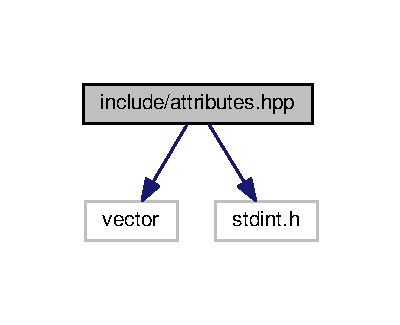
\includegraphics[width=192pt]{attributes_8hpp__incl}
\end{center}
\end{figure}
This graph shows which files directly or indirectly include this file\+:\nopagebreak
\begin{figure}[H]
\begin{center}
\leavevmode
\includegraphics[width=350pt]{attributes_8hpp__dep__incl}
\end{center}
\end{figure}
\subsection*{Classes}
\begin{DoxyCompactItemize}
\item 
struct \hyperlink{structConstantValue__attribute__s}{Constant\+Value\+\_\+attribute\+\_\+s}
\item 
struct \hyperlink{structSourceFile__attribute__s}{Source\+File\+\_\+attribute\+\_\+s}
\item 
struct \hyperlink{structSynthetic__attribute__s}{Synthetic\+\_\+attribute\+\_\+s}
\item 
struct \hyperlink{structexception__table__info__s}{exception\+\_\+table\+\_\+info\+\_\+s}
\item 
struct \hyperlink{structline__number__table__info__s}{line\+\_\+number\+\_\+table\+\_\+info\+\_\+s}
\item 
struct \hyperlink{structLineNumberTable__attribute__s}{Line\+Number\+Table\+\_\+attribute\+\_\+s}
\item 
struct \hyperlink{structlocal__variable__table__info__s}{local\+\_\+variable\+\_\+table\+\_\+info\+\_\+s}
\item 
struct \hyperlink{structLocalVariableTable__attribute__s}{Local\+Variable\+Table\+\_\+attribute\+\_\+s}
\item 
struct \hyperlink{structlocal__variable__type__table__info__s}{local\+\_\+variable\+\_\+type\+\_\+table\+\_\+info\+\_\+s}
\item 
struct \hyperlink{structLocalVariableTypeTable__attribute__s}{Local\+Variable\+Type\+Table\+\_\+attribute\+\_\+s}
\item 
struct \hyperlink{structCode__attribute__s}{Code\+\_\+attribute\+\_\+s}
\item 
struct \hyperlink{structclasses__info__s}{classes\+\_\+info\+\_\+s}
\item 
struct \hyperlink{structInnerClasses__attribute__s}{Inner\+Classes\+\_\+attribute\+\_\+s}
\item 
struct \hyperlink{structtions__attribute__s}{tions\+\_\+attribute\+\_\+s}
\item 
union \hyperlink{unionattribute__type__u}{attribute\+\_\+type\+\_\+u}
\item 
struct \hyperlink{structattribute__info__s}{attribute\+\_\+info\+\_\+s}
\item 
struct \hyperlink{structEnclosingMethod__attribute__s}{Enclosing\+Method\+\_\+attribute\+\_\+s}
\item 
struct \hyperlink{structSignature__attribute__s}{Signature\+\_\+attribute\+\_\+s}
\item 
struct \hyperlink{structDeprecated__attribute__s}{Deprecated\+\_\+attribute\+\_\+s}
\end{DoxyCompactItemize}
\subsection*{Typedefs}
\begin{DoxyCompactItemize}
\item 
typedef struct \\*
\hyperlink{structConstantValue__attribute__s}{Constant\+Value\+\_\+attribute\+\_\+s} \hyperlink{attributes_8hpp_a4df3241aeeb4382aa355a8c4e4e6076e}{Constant\+Value\+\_\+attribute}
\item 
typedef struct \\*
\hyperlink{structSourceFile__attribute__s}{Source\+File\+\_\+attribute\+\_\+s} \hyperlink{attributes_8hpp_a493a40fa668908ed61dbb1f823d213ca}{Source\+File\+\_\+attribute}
\item 
typedef struct \\*
\hyperlink{structSynthetic__attribute__s}{Synthetic\+\_\+attribute\+\_\+s} \hyperlink{attributes_8hpp_a7dfc4097d3a6cf1ac27bf4ac345e7c99}{Synthetic\+\_\+attribute}
\item 
typedef struct \\*
\hyperlink{structexception__table__info__s}{exception\+\_\+table\+\_\+info\+\_\+s} \hyperlink{attributes_8hpp_a558a3f6c08900fb98e1ab97c492cc41b}{exception\+\_\+table\+\_\+info}
\item 
typedef struct \\*
\hyperlink{structline__number__table__info__s}{line\+\_\+number\+\_\+table\+\_\+info\+\_\+s} \hyperlink{attributes_8hpp_a27b6c85369a912aa549462c1ede3cc99}{line\+\_\+number\+\_\+table\+\_\+info}
\item 
typedef struct \\*
\hyperlink{structLineNumberTable__attribute__s}{Line\+Number\+Table\+\_\+attribute\+\_\+s} \hyperlink{attributes_8hpp_af2b24f13bd3e5a26936bd16e72a76fff}{Line\+Number\+Table\+\_\+attribute}
\item 
typedef struct \\*
\hyperlink{structlocal__variable__table__info__s}{local\+\_\+variable\+\_\+table\+\_\+info\+\_\+s} \hyperlink{attributes_8hpp_ac0faec3264719598fb702dbf93bbd46f}{local\+\_\+variable\+\_\+table\+\_\+info}
\item 
typedef struct \\*
\hyperlink{structLocalVariableTable__attribute__s}{Local\+Variable\+Table\+\_\+attribute\+\_\+s} \hyperlink{attributes_8hpp_a2985a5f278e47c68777158d1feac4d4f}{Local\+Variable\+Table\+\_\+attribute}
\item 
typedef struct \\*
\hyperlink{structlocal__variable__type__table__info__s}{local\+\_\+variable\+\_\+type\+\_\+table\+\_\+info\+\_\+s} \hyperlink{attributes_8hpp_aa5d2134065f2de46fc36fad5e31190d4}{local\+\_\+variable\+\_\+type\+\_\+table\+\_\+info}
\item 
typedef struct \\*
\hyperlink{structLocalVariableTypeTable__attribute__s}{Local\+Variable\+Type\+Table\+\_\+attribute\+\_\+s} \hyperlink{attributes_8hpp_a5a25e5296f4e3d6a99598ff645e598f2}{Local\+Variable\+Type\+Table\+\_\+attribute}
\item 
typedef struct \hyperlink{structCode__attribute__s}{Code\+\_\+attribute\+\_\+s} \hyperlink{attributes_8hpp_ad1d2692bc09d9023430faad186e7647e}{Code\+\_\+attribute}
\item 
typedef struct \hyperlink{structclasses__info__s}{classes\+\_\+info\+\_\+s} \hyperlink{attributes_8hpp_ade4d95a56a50512b3a546ee948651078}{classes\+\_\+info}
\item 
typedef struct \\*
\hyperlink{structInnerClasses__attribute__s}{Inner\+Classes\+\_\+attribute\+\_\+s} \hyperlink{attributes_8hpp_a11c3b261bde2a1da5fc73081cf62b4db}{Inner\+Classes\+\_\+attribute}
\item 
typedef struct \hyperlink{structtions__attribute__s}{tions\+\_\+attribute\+\_\+s} \hyperlink{attributes_8hpp_a472ae3f91d9dfb17a0125bd633c0a3ce}{Exceptions\+\_\+attribute}
\item 
typedef union \hyperlink{unionattribute__type__u}{attribute\+\_\+type\+\_\+u} \hyperlink{attributes_8hpp_a1f6857b772af6ea7fc2f978b57567f0d}{attribute\+Type\+\_\+u}
\item 
typedef struct \hyperlink{structattribute__info__s}{attribute\+\_\+info\+\_\+s} \hyperlink{attributes_8hpp_a7af51299ff517acce960ac87c9db9899}{attribute\+\_\+info}
\item 
typedef struct \\*
\hyperlink{structEnclosingMethod__attribute__s}{Enclosing\+Method\+\_\+attribute\+\_\+s} \hyperlink{attributes_8hpp_aba5003bdf67cbf1bc671ca750c4b7e01}{Enclosing\+Method\+\_\+attribute}
\item 
typedef struct \\*
\hyperlink{structSignature__attribute__s}{Signature\+\_\+attribute\+\_\+s} \hyperlink{attributes_8hpp_a12d46a9314a53e714e1adf21f03f05a7}{Signature\+\_\+attribute}
\item 
typedef struct \\*
\hyperlink{structDeprecated__attribute__s}{Deprecated\+\_\+attribute\+\_\+s} \hyperlink{attributes_8hpp_a814188cf623bd1d44790aa05dd210134}{Deprecated\+\_\+attribute}
\end{DoxyCompactItemize}


\subsection{Typedef Documentation}
\hypertarget{attributes_8hpp_a7af51299ff517acce960ac87c9db9899}{\index{attributes.\+hpp@{attributes.\+hpp}!attribute\+\_\+info@{attribute\+\_\+info}}
\index{attribute\+\_\+info@{attribute\+\_\+info}!attributes.\+hpp@{attributes.\+hpp}}
\subsubsection[{attribute\+\_\+info}]{\setlength{\rightskip}{0pt plus 5cm}typedef struct {\bf attribute\+\_\+info\+\_\+s}  {\bf attribute\+\_\+info}}}\label{attributes_8hpp_a7af51299ff517acce960ac87c9db9899}
\hypertarget{attributes_8hpp_a1f6857b772af6ea7fc2f978b57567f0d}{\index{attributes.\+hpp@{attributes.\+hpp}!attribute\+Type\+\_\+u@{attribute\+Type\+\_\+u}}
\index{attribute\+Type\+\_\+u@{attribute\+Type\+\_\+u}!attributes.\+hpp@{attributes.\+hpp}}
\subsubsection[{attribute\+Type\+\_\+u}]{\setlength{\rightskip}{0pt plus 5cm}typedef union {\bf attribute\+\_\+type\+\_\+u}  {\bf attribute\+Type\+\_\+u}}}\label{attributes_8hpp_a1f6857b772af6ea7fc2f978b57567f0d}
\hypertarget{attributes_8hpp_ade4d95a56a50512b3a546ee948651078}{\index{attributes.\+hpp@{attributes.\+hpp}!classes\+\_\+info@{classes\+\_\+info}}
\index{classes\+\_\+info@{classes\+\_\+info}!attributes.\+hpp@{attributes.\+hpp}}
\subsubsection[{classes\+\_\+info}]{\setlength{\rightskip}{0pt plus 5cm}typedef struct {\bf classes\+\_\+info\+\_\+s}  {\bf classes\+\_\+info}}}\label{attributes_8hpp_ade4d95a56a50512b3a546ee948651078}
\hypertarget{attributes_8hpp_ad1d2692bc09d9023430faad186e7647e}{\index{attributes.\+hpp@{attributes.\+hpp}!Code\+\_\+attribute@{Code\+\_\+attribute}}
\index{Code\+\_\+attribute@{Code\+\_\+attribute}!attributes.\+hpp@{attributes.\+hpp}}
\subsubsection[{Code\+\_\+attribute}]{\setlength{\rightskip}{0pt plus 5cm}typedef struct {\bf Code\+\_\+attribute\+\_\+s}  {\bf Code\+\_\+attribute}}}\label{attributes_8hpp_ad1d2692bc09d9023430faad186e7647e}
\hypertarget{attributes_8hpp_a4df3241aeeb4382aa355a8c4e4e6076e}{\index{attributes.\+hpp@{attributes.\+hpp}!Constant\+Value\+\_\+attribute@{Constant\+Value\+\_\+attribute}}
\index{Constant\+Value\+\_\+attribute@{Constant\+Value\+\_\+attribute}!attributes.\+hpp@{attributes.\+hpp}}
\subsubsection[{Constant\+Value\+\_\+attribute}]{\setlength{\rightskip}{0pt plus 5cm}typedef struct {\bf Constant\+Value\+\_\+attribute\+\_\+s}  {\bf Constant\+Value\+\_\+attribute}}}\label{attributes_8hpp_a4df3241aeeb4382aa355a8c4e4e6076e}
\hypertarget{attributes_8hpp_a814188cf623bd1d44790aa05dd210134}{\index{attributes.\+hpp@{attributes.\+hpp}!Deprecated\+\_\+attribute@{Deprecated\+\_\+attribute}}
\index{Deprecated\+\_\+attribute@{Deprecated\+\_\+attribute}!attributes.\+hpp@{attributes.\+hpp}}
\subsubsection[{Deprecated\+\_\+attribute}]{\setlength{\rightskip}{0pt plus 5cm}typedef struct {\bf Deprecated\+\_\+attribute\+\_\+s}  {\bf Deprecated\+\_\+attribute}}}\label{attributes_8hpp_a814188cf623bd1d44790aa05dd210134}
\hypertarget{attributes_8hpp_aba5003bdf67cbf1bc671ca750c4b7e01}{\index{attributes.\+hpp@{attributes.\+hpp}!Enclosing\+Method\+\_\+attribute@{Enclosing\+Method\+\_\+attribute}}
\index{Enclosing\+Method\+\_\+attribute@{Enclosing\+Method\+\_\+attribute}!attributes.\+hpp@{attributes.\+hpp}}
\subsubsection[{Enclosing\+Method\+\_\+attribute}]{\setlength{\rightskip}{0pt plus 5cm}typedef struct {\bf Enclosing\+Method\+\_\+attribute\+\_\+s}  {\bf Enclosing\+Method\+\_\+attribute}}}\label{attributes_8hpp_aba5003bdf67cbf1bc671ca750c4b7e01}
\hypertarget{attributes_8hpp_a558a3f6c08900fb98e1ab97c492cc41b}{\index{attributes.\+hpp@{attributes.\+hpp}!exception\+\_\+table\+\_\+info@{exception\+\_\+table\+\_\+info}}
\index{exception\+\_\+table\+\_\+info@{exception\+\_\+table\+\_\+info}!attributes.\+hpp@{attributes.\+hpp}}
\subsubsection[{exception\+\_\+table\+\_\+info}]{\setlength{\rightskip}{0pt plus 5cm}typedef struct {\bf exception\+\_\+table\+\_\+info\+\_\+s}  {\bf exception\+\_\+table\+\_\+info}}}\label{attributes_8hpp_a558a3f6c08900fb98e1ab97c492cc41b}
\hypertarget{attributes_8hpp_a472ae3f91d9dfb17a0125bd633c0a3ce}{\index{attributes.\+hpp@{attributes.\+hpp}!Exceptions\+\_\+attribute@{Exceptions\+\_\+attribute}}
\index{Exceptions\+\_\+attribute@{Exceptions\+\_\+attribute}!attributes.\+hpp@{attributes.\+hpp}}
\subsubsection[{Exceptions\+\_\+attribute}]{\setlength{\rightskip}{0pt plus 5cm}typedef struct {\bf tions\+\_\+attribute\+\_\+s}  {\bf Exceptions\+\_\+attribute}}}\label{attributes_8hpp_a472ae3f91d9dfb17a0125bd633c0a3ce}
\hypertarget{attributes_8hpp_a11c3b261bde2a1da5fc73081cf62b4db}{\index{attributes.\+hpp@{attributes.\+hpp}!Inner\+Classes\+\_\+attribute@{Inner\+Classes\+\_\+attribute}}
\index{Inner\+Classes\+\_\+attribute@{Inner\+Classes\+\_\+attribute}!attributes.\+hpp@{attributes.\+hpp}}
\subsubsection[{Inner\+Classes\+\_\+attribute}]{\setlength{\rightskip}{0pt plus 5cm}typedef struct {\bf Inner\+Classes\+\_\+attribute\+\_\+s}  {\bf Inner\+Classes\+\_\+attribute}}}\label{attributes_8hpp_a11c3b261bde2a1da5fc73081cf62b4db}
\hypertarget{attributes_8hpp_a27b6c85369a912aa549462c1ede3cc99}{\index{attributes.\+hpp@{attributes.\+hpp}!line\+\_\+number\+\_\+table\+\_\+info@{line\+\_\+number\+\_\+table\+\_\+info}}
\index{line\+\_\+number\+\_\+table\+\_\+info@{line\+\_\+number\+\_\+table\+\_\+info}!attributes.\+hpp@{attributes.\+hpp}}
\subsubsection[{line\+\_\+number\+\_\+table\+\_\+info}]{\setlength{\rightskip}{0pt plus 5cm}typedef struct {\bf line\+\_\+number\+\_\+table\+\_\+info\+\_\+s}  {\bf line\+\_\+number\+\_\+table\+\_\+info}}}\label{attributes_8hpp_a27b6c85369a912aa549462c1ede3cc99}
\hypertarget{attributes_8hpp_af2b24f13bd3e5a26936bd16e72a76fff}{\index{attributes.\+hpp@{attributes.\+hpp}!Line\+Number\+Table\+\_\+attribute@{Line\+Number\+Table\+\_\+attribute}}
\index{Line\+Number\+Table\+\_\+attribute@{Line\+Number\+Table\+\_\+attribute}!attributes.\+hpp@{attributes.\+hpp}}
\subsubsection[{Line\+Number\+Table\+\_\+attribute}]{\setlength{\rightskip}{0pt plus 5cm}typedef struct {\bf Line\+Number\+Table\+\_\+attribute\+\_\+s}  {\bf Line\+Number\+Table\+\_\+attribute}}}\label{attributes_8hpp_af2b24f13bd3e5a26936bd16e72a76fff}
\hypertarget{attributes_8hpp_ac0faec3264719598fb702dbf93bbd46f}{\index{attributes.\+hpp@{attributes.\+hpp}!local\+\_\+variable\+\_\+table\+\_\+info@{local\+\_\+variable\+\_\+table\+\_\+info}}
\index{local\+\_\+variable\+\_\+table\+\_\+info@{local\+\_\+variable\+\_\+table\+\_\+info}!attributes.\+hpp@{attributes.\+hpp}}
\subsubsection[{local\+\_\+variable\+\_\+table\+\_\+info}]{\setlength{\rightskip}{0pt plus 5cm}typedef struct {\bf local\+\_\+variable\+\_\+table\+\_\+info\+\_\+s}  {\bf local\+\_\+variable\+\_\+table\+\_\+info}}}\label{attributes_8hpp_ac0faec3264719598fb702dbf93bbd46f}
\hypertarget{attributes_8hpp_aa5d2134065f2de46fc36fad5e31190d4}{\index{attributes.\+hpp@{attributes.\+hpp}!local\+\_\+variable\+\_\+type\+\_\+table\+\_\+info@{local\+\_\+variable\+\_\+type\+\_\+table\+\_\+info}}
\index{local\+\_\+variable\+\_\+type\+\_\+table\+\_\+info@{local\+\_\+variable\+\_\+type\+\_\+table\+\_\+info}!attributes.\+hpp@{attributes.\+hpp}}
\subsubsection[{local\+\_\+variable\+\_\+type\+\_\+table\+\_\+info}]{\setlength{\rightskip}{0pt plus 5cm}typedef struct {\bf local\+\_\+variable\+\_\+type\+\_\+table\+\_\+info\+\_\+s}  {\bf local\+\_\+variable\+\_\+type\+\_\+table\+\_\+info}}}\label{attributes_8hpp_aa5d2134065f2de46fc36fad5e31190d4}
\hypertarget{attributes_8hpp_a2985a5f278e47c68777158d1feac4d4f}{\index{attributes.\+hpp@{attributes.\+hpp}!Local\+Variable\+Table\+\_\+attribute@{Local\+Variable\+Table\+\_\+attribute}}
\index{Local\+Variable\+Table\+\_\+attribute@{Local\+Variable\+Table\+\_\+attribute}!attributes.\+hpp@{attributes.\+hpp}}
\subsubsection[{Local\+Variable\+Table\+\_\+attribute}]{\setlength{\rightskip}{0pt plus 5cm}typedef struct {\bf Local\+Variable\+Table\+\_\+attribute\+\_\+s}  {\bf Local\+Variable\+Table\+\_\+attribute}}}\label{attributes_8hpp_a2985a5f278e47c68777158d1feac4d4f}
\hypertarget{attributes_8hpp_a5a25e5296f4e3d6a99598ff645e598f2}{\index{attributes.\+hpp@{attributes.\+hpp}!Local\+Variable\+Type\+Table\+\_\+attribute@{Local\+Variable\+Type\+Table\+\_\+attribute}}
\index{Local\+Variable\+Type\+Table\+\_\+attribute@{Local\+Variable\+Type\+Table\+\_\+attribute}!attributes.\+hpp@{attributes.\+hpp}}
\subsubsection[{Local\+Variable\+Type\+Table\+\_\+attribute}]{\setlength{\rightskip}{0pt plus 5cm}typedef struct {\bf Local\+Variable\+Type\+Table\+\_\+attribute\+\_\+s}  {\bf Local\+Variable\+Type\+Table\+\_\+attribute}}}\label{attributes_8hpp_a5a25e5296f4e3d6a99598ff645e598f2}
\hypertarget{attributes_8hpp_a12d46a9314a53e714e1adf21f03f05a7}{\index{attributes.\+hpp@{attributes.\+hpp}!Signature\+\_\+attribute@{Signature\+\_\+attribute}}
\index{Signature\+\_\+attribute@{Signature\+\_\+attribute}!attributes.\+hpp@{attributes.\+hpp}}
\subsubsection[{Signature\+\_\+attribute}]{\setlength{\rightskip}{0pt plus 5cm}typedef struct {\bf Signature\+\_\+attribute\+\_\+s}  {\bf Signature\+\_\+attribute}}}\label{attributes_8hpp_a12d46a9314a53e714e1adf21f03f05a7}
\hypertarget{attributes_8hpp_a493a40fa668908ed61dbb1f823d213ca}{\index{attributes.\+hpp@{attributes.\+hpp}!Source\+File\+\_\+attribute@{Source\+File\+\_\+attribute}}
\index{Source\+File\+\_\+attribute@{Source\+File\+\_\+attribute}!attributes.\+hpp@{attributes.\+hpp}}
\subsubsection[{Source\+File\+\_\+attribute}]{\setlength{\rightskip}{0pt plus 5cm}typedef struct {\bf Source\+File\+\_\+attribute\+\_\+s}  {\bf Source\+File\+\_\+attribute}}}\label{attributes_8hpp_a493a40fa668908ed61dbb1f823d213ca}
\hypertarget{attributes_8hpp_a7dfc4097d3a6cf1ac27bf4ac345e7c99}{\index{attributes.\+hpp@{attributes.\+hpp}!Synthetic\+\_\+attribute@{Synthetic\+\_\+attribute}}
\index{Synthetic\+\_\+attribute@{Synthetic\+\_\+attribute}!attributes.\+hpp@{attributes.\+hpp}}
\subsubsection[{Synthetic\+\_\+attribute}]{\setlength{\rightskip}{0pt plus 5cm}typedef struct {\bf Synthetic\+\_\+attribute\+\_\+s}  {\bf Synthetic\+\_\+attribute}}}\label{attributes_8hpp_a7dfc4097d3a6cf1ac27bf4ac345e7c99}

\hypertarget{classFile_8hpp}{\section{include/class\+File.hpp File Reference}
\label{classFile_8hpp}\index{include/class\+File.\+hpp@{include/class\+File.\+hpp}}
}
{\ttfamily \#include $<$stdio.\+h$>$}\\*
{\ttfamily \#include $<$string.\+h$>$}\\*
{\ttfamily \#include $<$string$>$}\\*
{\ttfamily \#include $<$map$>$}\\*
{\ttfamily \#include $<$exception$>$}\\*
{\ttfamily \#include \char`\"{}../include/structs.\+hpp\char`\"{}}\\*
Include dependency graph for class\+File.\+hpp\+:\nopagebreak
\begin{figure}[H]
\begin{center}
\leavevmode
\includegraphics[width=350pt]{classFile_8hpp__incl}
\end{center}
\end{figure}
This graph shows which files directly or indirectly include this file\+:\nopagebreak
\begin{figure}[H]
\begin{center}
\leavevmode
\includegraphics[width=350pt]{classFile_8hpp__dep__incl}
\end{center}
\end{figure}
\subsection*{Classes}
\begin{DoxyCompactItemize}
\item 
class \hyperlink{classClassFile}{Class\+File}
\begin{DoxyCompactList}\small\item\em ver \href{https://docs.oracle.com/javase/specs/jvms/se7/html/jvms-4.html#jvms-4.4}{\tt https\+://docs.\+oracle.\+com/javase/specs/jvms/se7/html/jvms-\/4.\+html\#jvms-\/4.\+4} \end{DoxyCompactList}\end{DoxyCompactItemize}

\hypertarget{exibidor_8hpp}{\section{include/exibidor.hpp File Reference}
\label{exibidor_8hpp}\index{include/exibidor.\+hpp@{include/exibidor.\+hpp}}
}
{\ttfamily \#include $<$math.\+h$>$}\\*
{\ttfamily \#include $<$string.\+h$>$}\\*
{\ttfamily \#include $<$iostream$>$}\\*
{\ttfamily \#include $<$iomanip$>$}\\*
{\ttfamily \#include $<$stdio.\+h$>$}\\*
{\ttfamily \#include $<$stdint.\+h$>$}\\*
{\ttfamily \#include \char`\"{}../include/structs.\+hpp\char`\"{}}\\*
{\ttfamily \#include \char`\"{}../include/print\+\_\+code.\+hpp\char`\"{}}\\*
{\ttfamily \#include \char`\"{}../include/class\+File.\+hpp\char`\"{}}\\*
{\ttfamily \#include \char`\"{}../include/op\+\_\+instrucs.\+hpp\char`\"{}}\\*
{\ttfamily \#include \char`\"{}../include/operation\+Map.\+hpp\char`\"{}}\\*
Include dependency graph for exibidor.\+hpp\+:\nopagebreak
\begin{figure}[H]
\begin{center}
\leavevmode
\includegraphics[width=350pt]{exibidor_8hpp__incl}
\end{center}
\end{figure}
This graph shows which files directly or indirectly include this file\+:\nopagebreak
\begin{figure}[H]
\begin{center}
\leavevmode
\includegraphics[width=350pt]{exibidor_8hpp__dep__incl}
\end{center}
\end{figure}
\subsection*{Functions}
\begin{DoxyCompactItemize}
\item 
void \hyperlink{exibidor_8hpp_a1d672c700b6a228acb9d9d3fdd97b3f2}{exibe\+Class} (\hyperlink{classClassFile}{Class\+File} class\+F)
\item 
void \hyperlink{exibidor_8hpp_a103c8640faef4b3acd9d2a1c77efd61c}{print\+\_\+comment} (std\+::vector$<$ \hyperlink{structcp__info__s}{cp\+\_\+info\+\_\+s} $>$ c, int n)
\end{DoxyCompactItemize}


\subsection{Function Documentation}
\hypertarget{exibidor_8hpp_a1d672c700b6a228acb9d9d3fdd97b3f2}{\index{exibidor.\+hpp@{exibidor.\+hpp}!exibe\+Class@{exibe\+Class}}
\index{exibe\+Class@{exibe\+Class}!exibidor.\+hpp@{exibidor.\+hpp}}
\subsubsection[{exibe\+Class}]{\setlength{\rightskip}{0pt plus 5cm}void exibe\+Class (
\begin{DoxyParamCaption}
\item[{{\bf Class\+File}}]{class\+F}
\end{DoxyParamCaption}
)}}\label{exibidor_8hpp_a1d672c700b6a228acb9d9d3fdd97b3f2}
\hypertarget{exibidor_8hpp_a103c8640faef4b3acd9d2a1c77efd61c}{\index{exibidor.\+hpp@{exibidor.\+hpp}!print\+\_\+comment@{print\+\_\+comment}}
\index{print\+\_\+comment@{print\+\_\+comment}!exibidor.\+hpp@{exibidor.\+hpp}}
\subsubsection[{print\+\_\+comment}]{\setlength{\rightskip}{0pt plus 5cm}void print\+\_\+comment (
\begin{DoxyParamCaption}
\item[{std\+::vector$<$ {\bf cp\+\_\+info\+\_\+s} $>$}]{c, }
\item[{int}]{n}
\end{DoxyParamCaption}
)}}\label{exibidor_8hpp_a103c8640faef4b3acd9d2a1c77efd61c}

\hypertarget{frame_8hpp}{\section{include/frame.hpp File Reference}
\label{frame_8hpp}\index{include/frame.\+hpp@{include/frame.\+hpp}}
}


Define estruturas relacionados aos frames de execucao.  


{\ttfamily \#include $<$vector$>$}\\*
{\ttfamily \#include $<$cstdint$>$}\\*
{\ttfamily \#include $<$sstream$>$}\\*
{\ttfamily \#include $<$iostream$>$}\\*
{\ttfamily \#include \char`\"{}../include/heap.\+hpp\char`\"{}}\\*
Include dependency graph for frame.\+hpp\+:\nopagebreak
\begin{figure}[H]
\begin{center}
\leavevmode
\includegraphics[width=350pt]{frame_8hpp__incl}
\end{center}
\end{figure}
This graph shows which files directly or indirectly include this file\+:\nopagebreak
\begin{figure}[H]
\begin{center}
\leavevmode
\includegraphics[width=350pt]{frame_8hpp__dep__incl}
\end{center}
\end{figure}
\subsection*{Classes}
\begin{DoxyCompactItemize}
\item 
union \hyperlink{unionLocal__var__Type__u}{Local\+\_\+var\+\_\+\+Type\+\_\+u}
\item 
class \hyperlink{classLocal__var}{Local\+\_\+var}
\item 
class \hyperlink{classFrame}{Frame}
\end{DoxyCompactItemize}
\subsection*{Typedefs}
\begin{DoxyCompactItemize}
\item 
typedef union \hyperlink{unionLocal__var__Type__u}{Local\+\_\+var\+\_\+\+Type\+\_\+u} \hyperlink{frame_8hpp_ab261e63f0276830a985c2e9dc2b56b1c}{Local\+\_\+var\+\_\+\+Type}
\end{DoxyCompactItemize}


\subsection{Detailed Description}
Define estruturas relacionados aos frames de execucao. 



\subsection{Typedef Documentation}
\hypertarget{frame_8hpp_ab261e63f0276830a985c2e9dc2b56b1c}{\index{frame.\+hpp@{frame.\+hpp}!Local\+\_\+var\+\_\+\+Type@{Local\+\_\+var\+\_\+\+Type}}
\index{Local\+\_\+var\+\_\+\+Type@{Local\+\_\+var\+\_\+\+Type}!frame.\+hpp@{frame.\+hpp}}
\subsubsection[{Local\+\_\+var\+\_\+\+Type}]{\setlength{\rightskip}{0pt plus 5cm}typedef union {\bf Local\+\_\+var\+\_\+\+Type\+\_\+u} {\bf Local\+\_\+var\+\_\+\+Type}}}\label{frame_8hpp_ab261e63f0276830a985c2e9dc2b56b1c}

\hypertarget{heap_8hpp}{\section{include/heap.hpp File Reference}
\label{heap_8hpp}\index{include/heap.\+hpp@{include/heap.\+hpp}}
}


Este arquivo trata a documentacaoo 4.\+3.\+2 \href{https://docs.oracle.com/javase/specs/jvms/se7/html/jvms-4.html#jvms-4.3}{\tt https\+://docs.\+oracle.\+com/javase/specs/jvms/se7/html/jvms-\/4.\+html\#jvms-\/4.\+3}.  


{\ttfamily \#include $<$map$>$}\\*
{\ttfamily \#include $<$vector$>$}\\*
{\ttfamily \#include $<$string$>$}\\*
{\ttfamily \#include \char`\"{}../include/class\+File.\+hpp\char`\"{}}\\*
Include dependency graph for heap.\+hpp\+:\nopagebreak
\begin{figure}[H]
\begin{center}
\leavevmode
\includegraphics[width=350pt]{heap_8hpp__incl}
\end{center}
\end{figure}
This graph shows which files directly or indirectly include this file\+:\nopagebreak
\begin{figure}[H]
\begin{center}
\leavevmode
\includegraphics[width=350pt]{heap_8hpp__dep__incl}
\end{center}
\end{figure}
\subsection*{Classes}
\begin{DoxyCompactItemize}
\item 
union \hyperlink{unionbase__type__s}{base\+\_\+type\+\_\+s}
\item 
struct \hyperlink{structBaseType__s}{Base\+Type\+\_\+s}
\item 
struct \hyperlink{structObjectType__s}{Object\+Type\+\_\+s}
\item 
struct \hyperlink{structArrayType__s}{Array\+Type\+\_\+s}
\item 
union \hyperlink{unionFieldType__u}{Field\+Type\+\_\+u}
\item 
class \hyperlink{classFieldValue}{Field\+Value}
\begin{DoxyCompactList}\small\item\em Valor empacotado da representacao de uma classe ela pode ser dos tipos Base\+Type, Object\+Type e Array\+Type para mais informacoes visite \href{https://docs.oracle.com/javase/specs/jvms/se7/html/jvms-4.html#jvms-4.5}{\tt https\+://docs.\+oracle.\+com/javase/specs/jvms/se7/html/jvms-\/4.\+html\#jvms-\/4.\+5}. \end{DoxyCompactList}\item 
class \hyperlink{classInstanceClass}{Instance\+Class}
\begin{DoxyCompactList}\small\item\em Esta classe eh a instancia fisica de um objeto para isto ela o valor de todos fields dentro de si e um ponteiro para sua classfile para facilitar a manipualacao das referencias. \end{DoxyCompactList}\end{DoxyCompactItemize}
\subsection*{Typedefs}
\begin{DoxyCompactItemize}
\item 
typedef enum \hyperlink{heap_8hpp_ae83508426e652eaafd6ed60af394164e}{tag\+\_\+tipo\+\_\+e} \hyperlink{heap_8hpp_abae472b4761acff5c0e2e945a106d1a0}{tag\+\_\+\+Tipo}
\item 
typedef union \hyperlink{unionbase__type__s}{base\+\_\+type\+\_\+s} \hyperlink{heap_8hpp_a19f79bf7b0c34f691bdd56ae53f83c35}{Base\+Type\+\_\+u}
\item 
typedef struct \hyperlink{structBaseType__s}{Base\+Type\+\_\+s} \hyperlink{heap_8hpp_aea58c62b09d898b3bbab32faebe7fbae}{Base\+Type}
\item 
typedef struct \hyperlink{structObjectType__s}{Object\+Type\+\_\+s} \hyperlink{heap_8hpp_afb90a1260754c6e21d4b6610e1682d51}{Object\+Type}
\item 
typedef std\+::vector$<$ \hyperlink{classFieldValue}{Field\+Value} $>$ \hyperlink{heap_8hpp_a02f27b1f1856ad001bcd2be51cef4faf}{arrayref}
\item 
typedef struct \hyperlink{structArrayType__s}{Array\+Type\+\_\+s} \hyperlink{heap_8hpp_aa630024ee56aa81525646e18ddf60284}{Array\+Type}
\item 
typedef union \hyperlink{unionFieldType__u}{Field\+Type\+\_\+u} \hyperlink{heap_8hpp_a64fe1bf0d5bb9b0891062127bc036b49}{Field\+Type}
\end{DoxyCompactItemize}
\subsection*{Enumerations}
\begin{DoxyCompactItemize}
\item 
enum \hyperlink{heap_8hpp_ae83508426e652eaafd6ed60af394164e}{tag\+\_\+tipo\+\_\+e} \{ \\*
\hyperlink{heap_8hpp_ae83508426e652eaafd6ed60af394164eae663dbb8f8244e122acb5bd6b2c216e1}{B\+O\+O\+L} = 11, 
\hyperlink{heap_8hpp_ae83508426e652eaafd6ed60af394164eafd5a5f51ce25953f3db2c7e93eb7864a}{I\+N\+T} = 1, 
\hyperlink{heap_8hpp_ae83508426e652eaafd6ed60af394164ea4618cf21306b3c647741afa7ebefcab8}{C\+H\+A\+R} = 2, 
\hyperlink{heap_8hpp_ae83508426e652eaafd6ed60af394164eaa7f492d725033c06576ac4ba21007297}{B\+Y\+T\+E} = 3, 
\\*
\hyperlink{heap_8hpp_ae83508426e652eaafd6ed60af394164ea6f1397fe3c92c3c86d199b674d23be39}{L\+O\+N\+G\+O} = 4, 
\hyperlink{heap_8hpp_ae83508426e652eaafd6ed60af394164eafa6801f41f1d6d13464339d38f1c44c3}{P\+F\+L\+U\+T\+U\+A\+N\+T\+E} = 5, 
\hyperlink{heap_8hpp_ae83508426e652eaafd6ed60af394164eabe402f6f28e799b7f68b6c2928d0a5fa}{C\+U\+R\+T\+O} = 6, 
\hyperlink{heap_8hpp_ae83508426e652eaafd6ed60af394164ea227536a459b4bda01a188a726b75ef67}{D\+U\+P\+L\+O} = 7, 
\\*
\hyperlink{heap_8hpp_ae83508426e652eaafd6ed60af394164eaef271216bfc3a08b536bfc8bcbea92b0}{B\+A\+S\+E\+T\+Y\+P\+E} = 8, 
\hyperlink{heap_8hpp_ae83508426e652eaafd6ed60af394164ea1dc35745049317b1f7d826b4f14449b4}{O\+B\+J\+E\+C\+T\+T\+Y\+P\+E} = 9, 
\hyperlink{heap_8hpp_ae83508426e652eaafd6ed60af394164ea3886a5503646ad1e8cb6782c34ec6c96}{A\+R\+R\+A\+Y\+T\+Y\+P\+E} = 10, 
\hyperlink{heap_8hpp_ae83508426e652eaafd6ed60af394164ea4fb643bf7baa548cbe5d8634ac3190ee}{V\+O\+I\+D\+\_\+\+T} = 0, 
\\*
\hyperlink{heap_8hpp_ae83508426e652eaafd6ed60af394164eae1399f269e3800c5fd2341a1c0eff978}{R\+E\+T\+U\+R\+N\+\_\+\+A\+D\+D\+R\+E\+S\+S} = 12, 
\hyperlink{heap_8hpp_ae83508426e652eaafd6ed60af394164eae1717a5be2df5e14c96d51116b05d16d}{S\+T\+R\+I\+N\+G\+T\+Y\+P\+E} = 13
 \}
\end{DoxyCompactItemize}


\subsection{Detailed Description}
Este arquivo trata a documentacaoo 4.\+3.\+2 \href{https://docs.oracle.com/javase/specs/jvms/se7/html/jvms-4.html#jvms-4.3}{\tt https\+://docs.\+oracle.\+com/javase/specs/jvms/se7/html/jvms-\/4.\+html\#jvms-\/4.\+3}. 



\subsection{Typedef Documentation}
\hypertarget{heap_8hpp_a02f27b1f1856ad001bcd2be51cef4faf}{\index{heap.\+hpp@{heap.\+hpp}!arrayref@{arrayref}}
\index{arrayref@{arrayref}!heap.\+hpp@{heap.\+hpp}}
\subsubsection[{arrayref}]{\setlength{\rightskip}{0pt plus 5cm}typedef std\+::vector$<${\bf Field\+Value}$>$ {\bf arrayref}}}\label{heap_8hpp_a02f27b1f1856ad001bcd2be51cef4faf}
\hypertarget{heap_8hpp_aa630024ee56aa81525646e18ddf60284}{\index{heap.\+hpp@{heap.\+hpp}!Array\+Type@{Array\+Type}}
\index{Array\+Type@{Array\+Type}!heap.\+hpp@{heap.\+hpp}}
\subsubsection[{Array\+Type}]{\setlength{\rightskip}{0pt plus 5cm}typedef struct {\bf Array\+Type\+\_\+s} {\bf Array\+Type}}}\label{heap_8hpp_aa630024ee56aa81525646e18ddf60284}
\hypertarget{heap_8hpp_aea58c62b09d898b3bbab32faebe7fbae}{\index{heap.\+hpp@{heap.\+hpp}!Base\+Type@{Base\+Type}}
\index{Base\+Type@{Base\+Type}!heap.\+hpp@{heap.\+hpp}}
\subsubsection[{Base\+Type}]{\setlength{\rightskip}{0pt plus 5cm}typedef struct {\bf Base\+Type\+\_\+s} {\bf Base\+Type}}}\label{heap_8hpp_aea58c62b09d898b3bbab32faebe7fbae}
\hypertarget{heap_8hpp_a19f79bf7b0c34f691bdd56ae53f83c35}{\index{heap.\+hpp@{heap.\+hpp}!Base\+Type\+\_\+u@{Base\+Type\+\_\+u}}
\index{Base\+Type\+\_\+u@{Base\+Type\+\_\+u}!heap.\+hpp@{heap.\+hpp}}
\subsubsection[{Base\+Type\+\_\+u}]{\setlength{\rightskip}{0pt plus 5cm}typedef union {\bf base\+\_\+type\+\_\+s} {\bf Base\+Type\+\_\+u}}}\label{heap_8hpp_a19f79bf7b0c34f691bdd56ae53f83c35}
\hypertarget{heap_8hpp_a64fe1bf0d5bb9b0891062127bc036b49}{\index{heap.\+hpp@{heap.\+hpp}!Field\+Type@{Field\+Type}}
\index{Field\+Type@{Field\+Type}!heap.\+hpp@{heap.\+hpp}}
\subsubsection[{Field\+Type}]{\setlength{\rightskip}{0pt plus 5cm}typedef union {\bf Field\+Type\+\_\+u} {\bf Field\+Type}}}\label{heap_8hpp_a64fe1bf0d5bb9b0891062127bc036b49}
\hypertarget{heap_8hpp_afb90a1260754c6e21d4b6610e1682d51}{\index{heap.\+hpp@{heap.\+hpp}!Object\+Type@{Object\+Type}}
\index{Object\+Type@{Object\+Type}!heap.\+hpp@{heap.\+hpp}}
\subsubsection[{Object\+Type}]{\setlength{\rightskip}{0pt plus 5cm}typedef struct {\bf Object\+Type\+\_\+s} {\bf Object\+Type}}}\label{heap_8hpp_afb90a1260754c6e21d4b6610e1682d51}
\hypertarget{heap_8hpp_abae472b4761acff5c0e2e945a106d1a0}{\index{heap.\+hpp@{heap.\+hpp}!tag\+\_\+\+Tipo@{tag\+\_\+\+Tipo}}
\index{tag\+\_\+\+Tipo@{tag\+\_\+\+Tipo}!heap.\+hpp@{heap.\+hpp}}
\subsubsection[{tag\+\_\+\+Tipo}]{\setlength{\rightskip}{0pt plus 5cm}typedef enum {\bf tag\+\_\+tipo\+\_\+e} {\bf tag\+\_\+\+Tipo}}}\label{heap_8hpp_abae472b4761acff5c0e2e945a106d1a0}


\subsection{Enumeration Type Documentation}
\hypertarget{heap_8hpp_ae83508426e652eaafd6ed60af394164e}{\index{heap.\+hpp@{heap.\+hpp}!tag\+\_\+tipo\+\_\+e@{tag\+\_\+tipo\+\_\+e}}
\index{tag\+\_\+tipo\+\_\+e@{tag\+\_\+tipo\+\_\+e}!heap.\+hpp@{heap.\+hpp}}
\subsubsection[{tag\+\_\+tipo\+\_\+e}]{\setlength{\rightskip}{0pt plus 5cm}enum {\bf tag\+\_\+tipo\+\_\+e}}}\label{heap_8hpp_ae83508426e652eaafd6ed60af394164e}
\begin{Desc}
\item[Enumerator]\par
\begin{description}
\index{B\+O\+O\+L@{B\+O\+O\+L}!heap.\+hpp@{heap.\+hpp}}\index{heap.\+hpp@{heap.\+hpp}!B\+O\+O\+L@{B\+O\+O\+L}}\item[{\em 
\hypertarget{heap_8hpp_ae83508426e652eaafd6ed60af394164eae663dbb8f8244e122acb5bd6b2c216e1}{B\+O\+O\+L}\label{heap_8hpp_ae83508426e652eaafd6ed60af394164eae663dbb8f8244e122acb5bd6b2c216e1}
}]\index{I\+N\+T@{I\+N\+T}!heap.\+hpp@{heap.\+hpp}}\index{heap.\+hpp@{heap.\+hpp}!I\+N\+T@{I\+N\+T}}\item[{\em 
\hypertarget{heap_8hpp_ae83508426e652eaafd6ed60af394164eafd5a5f51ce25953f3db2c7e93eb7864a}{I\+N\+T}\label{heap_8hpp_ae83508426e652eaafd6ed60af394164eafd5a5f51ce25953f3db2c7e93eb7864a}
}]\index{C\+H\+A\+R@{C\+H\+A\+R}!heap.\+hpp@{heap.\+hpp}}\index{heap.\+hpp@{heap.\+hpp}!C\+H\+A\+R@{C\+H\+A\+R}}\item[{\em 
\hypertarget{heap_8hpp_ae83508426e652eaafd6ed60af394164ea4618cf21306b3c647741afa7ebefcab8}{C\+H\+A\+R}\label{heap_8hpp_ae83508426e652eaafd6ed60af394164ea4618cf21306b3c647741afa7ebefcab8}
}]\index{B\+Y\+T\+E@{B\+Y\+T\+E}!heap.\+hpp@{heap.\+hpp}}\index{heap.\+hpp@{heap.\+hpp}!B\+Y\+T\+E@{B\+Y\+T\+E}}\item[{\em 
\hypertarget{heap_8hpp_ae83508426e652eaafd6ed60af394164eaa7f492d725033c06576ac4ba21007297}{B\+Y\+T\+E}\label{heap_8hpp_ae83508426e652eaafd6ed60af394164eaa7f492d725033c06576ac4ba21007297}
}]\index{L\+O\+N\+G\+O@{L\+O\+N\+G\+O}!heap.\+hpp@{heap.\+hpp}}\index{heap.\+hpp@{heap.\+hpp}!L\+O\+N\+G\+O@{L\+O\+N\+G\+O}}\item[{\em 
\hypertarget{heap_8hpp_ae83508426e652eaafd6ed60af394164ea6f1397fe3c92c3c86d199b674d23be39}{L\+O\+N\+G\+O}\label{heap_8hpp_ae83508426e652eaafd6ed60af394164ea6f1397fe3c92c3c86d199b674d23be39}
}]\index{P\+F\+L\+U\+T\+U\+A\+N\+T\+E@{P\+F\+L\+U\+T\+U\+A\+N\+T\+E}!heap.\+hpp@{heap.\+hpp}}\index{heap.\+hpp@{heap.\+hpp}!P\+F\+L\+U\+T\+U\+A\+N\+T\+E@{P\+F\+L\+U\+T\+U\+A\+N\+T\+E}}\item[{\em 
\hypertarget{heap_8hpp_ae83508426e652eaafd6ed60af394164eafa6801f41f1d6d13464339d38f1c44c3}{P\+F\+L\+U\+T\+U\+A\+N\+T\+E}\label{heap_8hpp_ae83508426e652eaafd6ed60af394164eafa6801f41f1d6d13464339d38f1c44c3}
}]\index{C\+U\+R\+T\+O@{C\+U\+R\+T\+O}!heap.\+hpp@{heap.\+hpp}}\index{heap.\+hpp@{heap.\+hpp}!C\+U\+R\+T\+O@{C\+U\+R\+T\+O}}\item[{\em 
\hypertarget{heap_8hpp_ae83508426e652eaafd6ed60af394164eabe402f6f28e799b7f68b6c2928d0a5fa}{C\+U\+R\+T\+O}\label{heap_8hpp_ae83508426e652eaafd6ed60af394164eabe402f6f28e799b7f68b6c2928d0a5fa}
}]\index{D\+U\+P\+L\+O@{D\+U\+P\+L\+O}!heap.\+hpp@{heap.\+hpp}}\index{heap.\+hpp@{heap.\+hpp}!D\+U\+P\+L\+O@{D\+U\+P\+L\+O}}\item[{\em 
\hypertarget{heap_8hpp_ae83508426e652eaafd6ed60af394164ea227536a459b4bda01a188a726b75ef67}{D\+U\+P\+L\+O}\label{heap_8hpp_ae83508426e652eaafd6ed60af394164ea227536a459b4bda01a188a726b75ef67}
}]\index{B\+A\+S\+E\+T\+Y\+P\+E@{B\+A\+S\+E\+T\+Y\+P\+E}!heap.\+hpp@{heap.\+hpp}}\index{heap.\+hpp@{heap.\+hpp}!B\+A\+S\+E\+T\+Y\+P\+E@{B\+A\+S\+E\+T\+Y\+P\+E}}\item[{\em 
\hypertarget{heap_8hpp_ae83508426e652eaafd6ed60af394164eaef271216bfc3a08b536bfc8bcbea92b0}{B\+A\+S\+E\+T\+Y\+P\+E}\label{heap_8hpp_ae83508426e652eaafd6ed60af394164eaef271216bfc3a08b536bfc8bcbea92b0}
}]\index{O\+B\+J\+E\+C\+T\+T\+Y\+P\+E@{O\+B\+J\+E\+C\+T\+T\+Y\+P\+E}!heap.\+hpp@{heap.\+hpp}}\index{heap.\+hpp@{heap.\+hpp}!O\+B\+J\+E\+C\+T\+T\+Y\+P\+E@{O\+B\+J\+E\+C\+T\+T\+Y\+P\+E}}\item[{\em 
\hypertarget{heap_8hpp_ae83508426e652eaafd6ed60af394164ea1dc35745049317b1f7d826b4f14449b4}{O\+B\+J\+E\+C\+T\+T\+Y\+P\+E}\label{heap_8hpp_ae83508426e652eaafd6ed60af394164ea1dc35745049317b1f7d826b4f14449b4}
}]\index{A\+R\+R\+A\+Y\+T\+Y\+P\+E@{A\+R\+R\+A\+Y\+T\+Y\+P\+E}!heap.\+hpp@{heap.\+hpp}}\index{heap.\+hpp@{heap.\+hpp}!A\+R\+R\+A\+Y\+T\+Y\+P\+E@{A\+R\+R\+A\+Y\+T\+Y\+P\+E}}\item[{\em 
\hypertarget{heap_8hpp_ae83508426e652eaafd6ed60af394164ea3886a5503646ad1e8cb6782c34ec6c96}{A\+R\+R\+A\+Y\+T\+Y\+P\+E}\label{heap_8hpp_ae83508426e652eaafd6ed60af394164ea3886a5503646ad1e8cb6782c34ec6c96}
}]\index{V\+O\+I\+D\+\_\+\+T@{V\+O\+I\+D\+\_\+\+T}!heap.\+hpp@{heap.\+hpp}}\index{heap.\+hpp@{heap.\+hpp}!V\+O\+I\+D\+\_\+\+T@{V\+O\+I\+D\+\_\+\+T}}\item[{\em 
\hypertarget{heap_8hpp_ae83508426e652eaafd6ed60af394164ea4fb643bf7baa548cbe5d8634ac3190ee}{V\+O\+I\+D\+\_\+\+T}\label{heap_8hpp_ae83508426e652eaafd6ed60af394164ea4fb643bf7baa548cbe5d8634ac3190ee}
}]\index{R\+E\+T\+U\+R\+N\+\_\+\+A\+D\+D\+R\+E\+S\+S@{R\+E\+T\+U\+R\+N\+\_\+\+A\+D\+D\+R\+E\+S\+S}!heap.\+hpp@{heap.\+hpp}}\index{heap.\+hpp@{heap.\+hpp}!R\+E\+T\+U\+R\+N\+\_\+\+A\+D\+D\+R\+E\+S\+S@{R\+E\+T\+U\+R\+N\+\_\+\+A\+D\+D\+R\+E\+S\+S}}\item[{\em 
\hypertarget{heap_8hpp_ae83508426e652eaafd6ed60af394164eae1399f269e3800c5fd2341a1c0eff978}{R\+E\+T\+U\+R\+N\+\_\+\+A\+D\+D\+R\+E\+S\+S}\label{heap_8hpp_ae83508426e652eaafd6ed60af394164eae1399f269e3800c5fd2341a1c0eff978}
}]\index{S\+T\+R\+I\+N\+G\+T\+Y\+P\+E@{S\+T\+R\+I\+N\+G\+T\+Y\+P\+E}!heap.\+hpp@{heap.\+hpp}}\index{heap.\+hpp@{heap.\+hpp}!S\+T\+R\+I\+N\+G\+T\+Y\+P\+E@{S\+T\+R\+I\+N\+G\+T\+Y\+P\+E}}\item[{\em 
\hypertarget{heap_8hpp_ae83508426e652eaafd6ed60af394164eae1717a5be2df5e14c96d51116b05d16d}{S\+T\+R\+I\+N\+G\+T\+Y\+P\+E}\label{heap_8hpp_ae83508426e652eaafd6ed60af394164eae1717a5be2df5e14c96d51116b05d16d}
}]\end{description}
\end{Desc}

\hypertarget{interpretador_8hpp}{\section{include/interpretador.hpp File Reference}
\label{interpretador_8hpp}\index{include/interpretador.\+hpp@{include/interpretador.\+hpp}}
}


Estruturas de interpretacao dos opcodes.  


{\ttfamily \#include $<$cstdint$>$}\\*
{\ttfamily \#include $<$tuple$>$}\\*
{\ttfamily \#include $<$stdio.\+h$>$}\\*
{\ttfamily \#include $<$stdlib.\+h$>$}\\*
{\ttfamily \#include $<$algorithm$>$}\\*
{\ttfamily \#include $<$math.\+h$>$}\\*
{\ttfamily \#include \char`\"{}../include/frame.\+hpp\char`\"{}}\\*
{\ttfamily \#include \char`\"{}../include/opcode.\+hpp\char`\"{}}\\*
{\ttfamily \#include \char`\"{}../include/jvm.\+hpp\char`\"{}}\\*
{\ttfamily \#include \char`\"{}../include/structs.\+hpp\char`\"{}}\\*
{\ttfamily \#include \char`\"{}../include/class\+File.\+hpp\char`\"{}}\\*
{\ttfamily \#include \char`\"{}../include/operation\+Map.\+hpp\char`\"{}}\\*
{\ttfamily \#include \char`\"{}../include/debug.\+hpp\char`\"{}}\\*
Include dependency graph for interpretador.\+hpp\+:
\nopagebreak
\begin{figure}[H]
\begin{center}
\leavevmode
\includegraphics[width=350pt]{interpretador_8hpp__incl}
\end{center}
\end{figure}
This graph shows which files directly or indirectly include this file\+:\nopagebreak
\begin{figure}[H]
\begin{center}
\leavevmode
\includegraphics[width=350pt]{interpretador_8hpp__dep__incl}
\end{center}
\end{figure}
\subsection*{Classes}
\begin{DoxyCompactItemize}
\item 
class \hyperlink{classInterpretador}{Interpretador}
\begin{DoxyCompactList}\small\item\em Responsavel por receber um frame e rodar as instrucoes contidas ali. \end{DoxyCompactList}\end{DoxyCompactItemize}
\subsection*{Macros}
\begin{DoxyCompactItemize}
\item 
\#define \hyperlink{interpretador_8hpp_ac0dea6770549fe97ecf21cf2f923d7fb}{num\+Opcodes}~250
\end{DoxyCompactItemize}


\subsection{Detailed Description}
Estruturas de interpretacao dos opcodes. 



\subsection{Macro Definition Documentation}
\hypertarget{interpretador_8hpp_ac0dea6770549fe97ecf21cf2f923d7fb}{\index{interpretador.\+hpp@{interpretador.\+hpp}!num\+Opcodes@{num\+Opcodes}}
\index{num\+Opcodes@{num\+Opcodes}!interpretador.\+hpp@{interpretador.\+hpp}}
\subsubsection[{num\+Opcodes}]{\setlength{\rightskip}{0pt plus 5cm}\#define num\+Opcodes~250}}\label{interpretador_8hpp_ac0dea6770549fe97ecf21cf2f923d7fb}

\hypertarget{interpreter__op__code_8hpp}{\section{include/interpreter\+\_\+op\+\_\+code.hpp File Reference}
\label{interpreter__op__code_8hpp}\index{include/interpreter\+\_\+op\+\_\+code.\+hpp@{include/interpreter\+\_\+op\+\_\+code.\+hpp}}
}
{\ttfamily \#include $<$stdint.\+h$>$}\\*
{\ttfamily \#include \char`\"{}../include/opcode.\+hpp\char`\"{}}\\*
{\ttfamily \#include $<$stdio.\+h$>$}\\*
Include dependency graph for interpreter\+\_\+op\+\_\+code.\+hpp\+:\nopagebreak
\begin{figure}[H]
\begin{center}
\leavevmode
\includegraphics[width=321pt]{interpreter__op__code_8hpp__incl}
\end{center}
\end{figure}
This graph shows which files directly or indirectly include this file\+:\nopagebreak
\begin{figure}[H]
\begin{center}
\leavevmode
\includegraphics[width=350pt]{interpreter__op__code_8hpp__dep__incl}
\end{center}
\end{figure}
\subsection*{Functions}
\begin{DoxyCompactItemize}
\item 
int \hyperlink{interpreter__op__code_8hpp_a8163804071b2e335efe422cc746c3e53}{interpreter\+\_\+op\+\_\+code} (uint8\+\_\+t opcode)
\end{DoxyCompactItemize}


\subsection{Function Documentation}
\hypertarget{interpreter__op__code_8hpp_a8163804071b2e335efe422cc746c3e53}{\index{interpreter\+\_\+op\+\_\+code.\+hpp@{interpreter\+\_\+op\+\_\+code.\+hpp}!interpreter\+\_\+op\+\_\+code@{interpreter\+\_\+op\+\_\+code}}
\index{interpreter\+\_\+op\+\_\+code@{interpreter\+\_\+op\+\_\+code}!interpreter\+\_\+op\+\_\+code.\+hpp@{interpreter\+\_\+op\+\_\+code.\+hpp}}
\subsubsection[{interpreter\+\_\+op\+\_\+code}]{\setlength{\rightskip}{0pt plus 5cm}int interpreter\+\_\+op\+\_\+code (
\begin{DoxyParamCaption}
\item[{uint8\+\_\+t}]{opcode}
\end{DoxyParamCaption}
)}}\label{interpreter__op__code_8hpp_a8163804071b2e335efe422cc746c3e53}

\hypertarget{jvm_8hpp}{\section{include/jvm.hpp File Reference}
\label{jvm_8hpp}\index{include/jvm.\+hpp@{include/jvm.\+hpp}}
}
{\ttfamily \#include $<$iostream$>$}\\*
{\ttfamily \#include \char`\"{}../include/leitor.\+hpp\char`\"{}}\\*
{\ttfamily \#include \char`\"{}../include/heap.\+hpp\char`\"{}}\\*
{\ttfamily \#include \char`\"{}../include/frame.\+hpp\char`\"{}}\\*
{\ttfamily \#include \char`\"{}../include/interpretador.\+hpp\char`\"{}}\\*
{\ttfamily \#include \char`\"{}../include/opcode.\+hpp\char`\"{}}\\*
{\ttfamily \#include \char`\"{}../include/exibidor.\+hpp\char`\"{}}\\*
{\ttfamily \#include \char`\"{}../include/class\+File.\+hpp\char`\"{}}\\*
{\ttfamily \#include \char`\"{}../include/op\+\_\+instrucs.\+hpp\char`\"{}}\\*
{\ttfamily \#include \char`\"{}../include/interpreter\+\_\+op\+\_\+code.\+hpp\char`\"{}}\\*
Include dependency graph for jvm.\+hpp\+:\nopagebreak
\begin{figure}[H]
\begin{center}
\leavevmode
\includegraphics[width=350pt]{jvm_8hpp__incl}
\end{center}
\end{figure}
This graph shows which files directly or indirectly include this file\+:\nopagebreak
\begin{figure}[H]
\begin{center}
\leavevmode
\includegraphics[width=350pt]{jvm_8hpp__dep__incl}
\end{center}
\end{figure}
\subsection*{Classes}
\begin{DoxyCompactItemize}
\item 
class \hyperlink{classJvm}{Jvm}
\begin{DoxyCompactList}\small\item\em Esta é a classe mãe da J\+V\+M ela Ela quem deve encontrar a main da classe inicial e rodar o loop para rodar os métodos. \end{DoxyCompactList}\end{DoxyCompactItemize}

\hypertarget{leitor_8hpp}{\section{include/leitor.hpp File Reference}
\label{leitor_8hpp}\index{include/leitor.\+hpp@{include/leitor.\+hpp}}
}
{\ttfamily \#include $<$stdlib.\+h$>$}\\*
{\ttfamily \#include $<$stdio.\+h$>$}\\*
{\ttfamily \#include $<$stdint.\+h$>$}\\*
{\ttfamily \#include $<$string$>$}\\*
{\ttfamily \#include $<$cstring$>$}\\*
{\ttfamily \#include \char`\"{}../include/structs.\+hpp\char`\"{}}\\*
{\ttfamily \#include \char`\"{}../include/class\+File.\+hpp\char`\"{}}\\*
{\ttfamily \#include \char`\"{}../include/attributes.\+hpp\char`\"{}}\\*
{\ttfamily \#include \char`\"{}../include/little\+\_\+to\+\_\+big.\+hpp\char`\"{}}\\*
{\ttfamily \#include \char`\"{}../include/read\+\_\+bytes.\+hpp\char`\"{}}\\*
{\ttfamily \#include \char`\"{}../include/read\+\_\+attributes.\+hpp\char`\"{}}\\*
{\ttfamily \#include \char`\"{}../include/read\+\_\+methods.\+hpp\char`\"{}}\\*
Include dependency graph for leitor.\+hpp\+:\nopagebreak
\begin{figure}[H]
\begin{center}
\leavevmode
\includegraphics[width=350pt]{leitor_8hpp__incl}
\end{center}
\end{figure}
This graph shows which files directly or indirectly include this file\+:
\nopagebreak
\begin{figure}[H]
\begin{center}
\leavevmode
\includegraphics[width=350pt]{leitor_8hpp__dep__incl}
\end{center}
\end{figure}
\subsection*{Macros}
\begin{DoxyCompactItemize}
\item 
\#define \hyperlink{leitor_8hpp_a261f9244a94a48446a55251bb8b274e5}{Byte\+Code}~\char`\"{}Puppy.\+class\char`\"{}
\item 
\#define \hyperlink{leitor_8hpp_a6fe20e564479ba3ea1501ae417ea7976}{File\+Name\+Len}~30
\end{DoxyCompactItemize}
\subsection*{Functions}
\begin{DoxyCompactItemize}
\item 
F\+I\+L\+E $\ast$ \hyperlink{leitor_8hpp_abd065d60349e13ce48be81c0a6bb30cf}{abre\+Arq\+Linha\+Comando} (int argc, char $\ast$$\ast$argv)
\item 
F\+I\+L\+E $\ast$ \hyperlink{leitor_8hpp_a3a9cf377fc510333e67bfbd1cef74c16}{abre\+Arquivo} (char $\ast$arquivo\+Java)
\item 
int \hyperlink{leitor_8hpp_a6df828bb880057ae6fb70042873df908}{leitor\+Class\+\_\+info} (\hyperlink{classClassFile}{Class\+File} $\ast$class\+F, F\+I\+L\+E $\ast$arquivo\+Java)
\item 
int \hyperlink{leitor_8hpp_a8b5c019846b3992988493818f1493c92}{leitura\+Header} (\hyperlink{classClassFile}{Class\+File} $\ast$class\+F, F\+I\+L\+E $\ast$arquivo\+Java)
\item 
int \hyperlink{leitor_8hpp_a51daaac319fb9374ab881006b1535b0a}{leitura\+Constant\+Pool} (\hyperlink{classClassFile}{Class\+File} $\ast$class\+F, F\+I\+L\+E $\ast$arquivo\+Java)
\item 
int \hyperlink{leitor_8hpp_aa0e8c879b9def6a71713c76b665ddb40}{leitura\+Access\+This\+Super} (\hyperlink{classClassFile}{Class\+File} $\ast$class\+F, F\+I\+L\+E $\ast$arquivo\+Java)
\item 
int \hyperlink{leitor_8hpp_a3c9c0e4833858b2c9a7eda0eeed059bb}{leitura\+Interfaces} (\hyperlink{classClassFile}{Class\+File} $\ast$class\+F, F\+I\+L\+E $\ast$arquivo\+Java)
\item 
int \hyperlink{leitor_8hpp_a667190e5f2e01151dd27529ec5d2770a}{leitura\+Fields} (\hyperlink{classClassFile}{Class\+File} $\ast$class\+F, F\+I\+L\+E $\ast$arquivo\+Java)
\item 
int \hyperlink{leitor_8hpp_ac9405ebb177dc540b19ccbf58fb341bd}{leitura\+Methods} (\hyperlink{classClassFile}{Class\+File} $\ast$class\+F, F\+I\+L\+E $\ast$arquivo\+Java)
\item 
int \hyperlink{leitor_8hpp_a6c2d3b25b34fba477bae0f739ffee71f}{leitura\+Attributes} (\hyperlink{classClassFile}{Class\+File} $\ast$class\+F, F\+I\+L\+E $\ast$arquivo\+Java)
\item 
char $\ast$ \hyperlink{leitor_8hpp_a1c0845a2189f3e3ddaf0e33c9a1ded80}{get\+Class\+Name} (\hyperlink{classClassFile}{Class\+File} $\ast$class\+F)
\end{DoxyCompactItemize}


\subsection{Macro Definition Documentation}
\hypertarget{leitor_8hpp_a261f9244a94a48446a55251bb8b274e5}{\index{leitor.\+hpp@{leitor.\+hpp}!Byte\+Code@{Byte\+Code}}
\index{Byte\+Code@{Byte\+Code}!leitor.\+hpp@{leitor.\+hpp}}
\subsubsection[{Byte\+Code}]{\setlength{\rightskip}{0pt plus 5cm}\#define Byte\+Code~\char`\"{}Puppy.\+class\char`\"{}}}\label{leitor_8hpp_a261f9244a94a48446a55251bb8b274e5}
\hypertarget{leitor_8hpp_a6fe20e564479ba3ea1501ae417ea7976}{\index{leitor.\+hpp@{leitor.\+hpp}!File\+Name\+Len@{File\+Name\+Len}}
\index{File\+Name\+Len@{File\+Name\+Len}!leitor.\+hpp@{leitor.\+hpp}}
\subsubsection[{File\+Name\+Len}]{\setlength{\rightskip}{0pt plus 5cm}\#define File\+Name\+Len~30}}\label{leitor_8hpp_a6fe20e564479ba3ea1501ae417ea7976}


\subsection{Function Documentation}
\hypertarget{leitor_8hpp_abd065d60349e13ce48be81c0a6bb30cf}{\index{leitor.\+hpp@{leitor.\+hpp}!abre\+Arq\+Linha\+Comando@{abre\+Arq\+Linha\+Comando}}
\index{abre\+Arq\+Linha\+Comando@{abre\+Arq\+Linha\+Comando}!leitor.\+hpp@{leitor.\+hpp}}
\subsubsection[{abre\+Arq\+Linha\+Comando}]{\setlength{\rightskip}{0pt plus 5cm}F\+I\+L\+E$\ast$ abre\+Arq\+Linha\+Comando (
\begin{DoxyParamCaption}
\item[{int}]{argc, }
\item[{char $\ast$$\ast$}]{argv}
\end{DoxyParamCaption}
)}}\label{leitor_8hpp_abd065d60349e13ce48be81c0a6bb30cf}
\hypertarget{leitor_8hpp_a3a9cf377fc510333e67bfbd1cef74c16}{\index{leitor.\+hpp@{leitor.\+hpp}!abre\+Arquivo@{abre\+Arquivo}}
\index{abre\+Arquivo@{abre\+Arquivo}!leitor.\+hpp@{leitor.\+hpp}}
\subsubsection[{abre\+Arquivo}]{\setlength{\rightskip}{0pt plus 5cm}F\+I\+L\+E$\ast$ abre\+Arquivo (
\begin{DoxyParamCaption}
\item[{char $\ast$}]{arquivo\+Java}
\end{DoxyParamCaption}
)}}\label{leitor_8hpp_a3a9cf377fc510333e67bfbd1cef74c16}
\hypertarget{leitor_8hpp_a1c0845a2189f3e3ddaf0e33c9a1ded80}{\index{leitor.\+hpp@{leitor.\+hpp}!get\+Class\+Name@{get\+Class\+Name}}
\index{get\+Class\+Name@{get\+Class\+Name}!leitor.\+hpp@{leitor.\+hpp}}
\subsubsection[{get\+Class\+Name}]{\setlength{\rightskip}{0pt plus 5cm}char$\ast$ get\+Class\+Name (
\begin{DoxyParamCaption}
\item[{{\bf Class\+File} $\ast$}]{class\+F}
\end{DoxyParamCaption}
)}}\label{leitor_8hpp_a1c0845a2189f3e3ddaf0e33c9a1ded80}
\hypertarget{leitor_8hpp_a6df828bb880057ae6fb70042873df908}{\index{leitor.\+hpp@{leitor.\+hpp}!leitor\+Class\+\_\+info@{leitor\+Class\+\_\+info}}
\index{leitor\+Class\+\_\+info@{leitor\+Class\+\_\+info}!leitor.\+hpp@{leitor.\+hpp}}
\subsubsection[{leitor\+Class\+\_\+info}]{\setlength{\rightskip}{0pt plus 5cm}int leitor\+Class\+\_\+info (
\begin{DoxyParamCaption}
\item[{{\bf Class\+File} $\ast$}]{class\+F, }
\item[{F\+I\+L\+E $\ast$}]{arquivo\+Java}
\end{DoxyParamCaption}
)}}\label{leitor_8hpp_a6df828bb880057ae6fb70042873df908}
\hypertarget{leitor_8hpp_aa0e8c879b9def6a71713c76b665ddb40}{\index{leitor.\+hpp@{leitor.\+hpp}!leitura\+Access\+This\+Super@{leitura\+Access\+This\+Super}}
\index{leitura\+Access\+This\+Super@{leitura\+Access\+This\+Super}!leitor.\+hpp@{leitor.\+hpp}}
\subsubsection[{leitura\+Access\+This\+Super}]{\setlength{\rightskip}{0pt plus 5cm}int leitura\+Access\+This\+Super (
\begin{DoxyParamCaption}
\item[{{\bf Class\+File} $\ast$}]{class\+F, }
\item[{F\+I\+L\+E $\ast$}]{arquivo\+Java}
\end{DoxyParamCaption}
)}}\label{leitor_8hpp_aa0e8c879b9def6a71713c76b665ddb40}
\hypertarget{leitor_8hpp_a6c2d3b25b34fba477bae0f739ffee71f}{\index{leitor.\+hpp@{leitor.\+hpp}!leitura\+Attributes@{leitura\+Attributes}}
\index{leitura\+Attributes@{leitura\+Attributes}!leitor.\+hpp@{leitor.\+hpp}}
\subsubsection[{leitura\+Attributes}]{\setlength{\rightskip}{0pt plus 5cm}int leitura\+Attributes (
\begin{DoxyParamCaption}
\item[{{\bf Class\+File} $\ast$}]{class\+F, }
\item[{F\+I\+L\+E $\ast$}]{arquivo\+Java}
\end{DoxyParamCaption}
)}}\label{leitor_8hpp_a6c2d3b25b34fba477bae0f739ffee71f}
\hypertarget{leitor_8hpp_a51daaac319fb9374ab881006b1535b0a}{\index{leitor.\+hpp@{leitor.\+hpp}!leitura\+Constant\+Pool@{leitura\+Constant\+Pool}}
\index{leitura\+Constant\+Pool@{leitura\+Constant\+Pool}!leitor.\+hpp@{leitor.\+hpp}}
\subsubsection[{leitura\+Constant\+Pool}]{\setlength{\rightskip}{0pt plus 5cm}int leitura\+Constant\+Pool (
\begin{DoxyParamCaption}
\item[{{\bf Class\+File} $\ast$}]{class\+F, }
\item[{F\+I\+L\+E $\ast$}]{arquivo\+Java}
\end{DoxyParamCaption}
)}}\label{leitor_8hpp_a51daaac319fb9374ab881006b1535b0a}
\hypertarget{leitor_8hpp_a667190e5f2e01151dd27529ec5d2770a}{\index{leitor.\+hpp@{leitor.\+hpp}!leitura\+Fields@{leitura\+Fields}}
\index{leitura\+Fields@{leitura\+Fields}!leitor.\+hpp@{leitor.\+hpp}}
\subsubsection[{leitura\+Fields}]{\setlength{\rightskip}{0pt plus 5cm}int leitura\+Fields (
\begin{DoxyParamCaption}
\item[{{\bf Class\+File} $\ast$}]{class\+F, }
\item[{F\+I\+L\+E $\ast$}]{arquivo\+Java}
\end{DoxyParamCaption}
)}}\label{leitor_8hpp_a667190e5f2e01151dd27529ec5d2770a}
\hypertarget{leitor_8hpp_a8b5c019846b3992988493818f1493c92}{\index{leitor.\+hpp@{leitor.\+hpp}!leitura\+Header@{leitura\+Header}}
\index{leitura\+Header@{leitura\+Header}!leitor.\+hpp@{leitor.\+hpp}}
\subsubsection[{leitura\+Header}]{\setlength{\rightskip}{0pt plus 5cm}int leitura\+Header (
\begin{DoxyParamCaption}
\item[{{\bf Class\+File} $\ast$}]{class\+F, }
\item[{F\+I\+L\+E $\ast$}]{arquivo\+Java}
\end{DoxyParamCaption}
)}}\label{leitor_8hpp_a8b5c019846b3992988493818f1493c92}
\hypertarget{leitor_8hpp_a3c9c0e4833858b2c9a7eda0eeed059bb}{\index{leitor.\+hpp@{leitor.\+hpp}!leitura\+Interfaces@{leitura\+Interfaces}}
\index{leitura\+Interfaces@{leitura\+Interfaces}!leitor.\+hpp@{leitor.\+hpp}}
\subsubsection[{leitura\+Interfaces}]{\setlength{\rightskip}{0pt plus 5cm}int leitura\+Interfaces (
\begin{DoxyParamCaption}
\item[{{\bf Class\+File} $\ast$}]{class\+F, }
\item[{F\+I\+L\+E $\ast$}]{arquivo\+Java}
\end{DoxyParamCaption}
)}}\label{leitor_8hpp_a3c9c0e4833858b2c9a7eda0eeed059bb}
\hypertarget{leitor_8hpp_ac9405ebb177dc540b19ccbf58fb341bd}{\index{leitor.\+hpp@{leitor.\+hpp}!leitura\+Methods@{leitura\+Methods}}
\index{leitura\+Methods@{leitura\+Methods}!leitor.\+hpp@{leitor.\+hpp}}
\subsubsection[{leitura\+Methods}]{\setlength{\rightskip}{0pt plus 5cm}int leitura\+Methods (
\begin{DoxyParamCaption}
\item[{{\bf Class\+File} $\ast$}]{class\+F, }
\item[{F\+I\+L\+E $\ast$}]{arquivo\+Java}
\end{DoxyParamCaption}
)}}\label{leitor_8hpp_ac9405ebb177dc540b19ccbf58fb341bd}

\hypertarget{little__to__big_8hpp}{\section{include/little\+\_\+to\+\_\+big.hpp File Reference}
\label{little__to__big_8hpp}\index{include/little\+\_\+to\+\_\+big.\+hpp@{include/little\+\_\+to\+\_\+big.\+hpp}}
}
{\ttfamily \#include $<$stdint.\+h$>$}\\*
Include dependency graph for little\+\_\+to\+\_\+big.\+hpp\+:\nopagebreak
\begin{figure}[H]
\begin{center}
\leavevmode
\includegraphics[width=198pt]{little__to__big_8hpp__incl}
\end{center}
\end{figure}
This graph shows which files directly or indirectly include this file\+:
\nopagebreak
\begin{figure}[H]
\begin{center}
\leavevmode
\includegraphics[width=350pt]{little__to__big_8hpp__dep__incl}
\end{center}
\end{figure}
\subsection*{Functions}
\begin{DoxyCompactItemize}
\item 
uint16\+\_\+t \hyperlink{little__to__big_8hpp_a2765a758d55894ff27a67210ecf8e220}{little\+\_\+to\+\_\+big16} (uint16\+\_\+t x)
\item 
uint32\+\_\+t \hyperlink{little__to__big_8hpp_ab3a7e43a3af2ba585bf2bc156af89116}{little\+\_\+to\+\_\+big32} (uint32\+\_\+t x)
\end{DoxyCompactItemize}


\subsection{Function Documentation}
\hypertarget{little__to__big_8hpp_a2765a758d55894ff27a67210ecf8e220}{\index{little\+\_\+to\+\_\+big.\+hpp@{little\+\_\+to\+\_\+big.\+hpp}!little\+\_\+to\+\_\+big16@{little\+\_\+to\+\_\+big16}}
\index{little\+\_\+to\+\_\+big16@{little\+\_\+to\+\_\+big16}!little\+\_\+to\+\_\+big.\+hpp@{little\+\_\+to\+\_\+big.\+hpp}}
\subsubsection[{little\+\_\+to\+\_\+big16}]{\setlength{\rightskip}{0pt plus 5cm}uint16\+\_\+t little\+\_\+to\+\_\+big16 (
\begin{DoxyParamCaption}
\item[{uint16\+\_\+t}]{x}
\end{DoxyParamCaption}
)}}\label{little__to__big_8hpp_a2765a758d55894ff27a67210ecf8e220}
\hypertarget{little__to__big_8hpp_ab3a7e43a3af2ba585bf2bc156af89116}{\index{little\+\_\+to\+\_\+big.\+hpp@{little\+\_\+to\+\_\+big.\+hpp}!little\+\_\+to\+\_\+big32@{little\+\_\+to\+\_\+big32}}
\index{little\+\_\+to\+\_\+big32@{little\+\_\+to\+\_\+big32}!little\+\_\+to\+\_\+big.\+hpp@{little\+\_\+to\+\_\+big.\+hpp}}
\subsubsection[{little\+\_\+to\+\_\+big32}]{\setlength{\rightskip}{0pt plus 5cm}uint32\+\_\+t little\+\_\+to\+\_\+big32 (
\begin{DoxyParamCaption}
\item[{uint32\+\_\+t}]{x}
\end{DoxyParamCaption}
)}}\label{little__to__big_8hpp_ab3a7e43a3af2ba585bf2bc156af89116}

\hypertarget{op__instrucs_8hpp}{\section{include/op\+\_\+instrucs.hpp File Reference}
\label{op__instrucs_8hpp}\index{include/op\+\_\+instrucs.\+hpp@{include/op\+\_\+instrucs.\+hpp}}
}
{\ttfamily \#include $<$map$>$}\\*
Include dependency graph for op\+\_\+instrucs.\+hpp\+:\nopagebreak
\begin{figure}[H]
\begin{center}
\leavevmode
\includegraphics[width=198pt]{op__instrucs_8hpp__incl}
\end{center}
\end{figure}
This graph shows which files directly or indirectly include this file\+:\nopagebreak
\begin{figure}[H]
\begin{center}
\leavevmode
\includegraphics[width=350pt]{op__instrucs_8hpp__dep__incl}
\end{center}
\end{figure}
\subsection*{Classes}
\begin{DoxyCompactItemize}
\item 
class \hyperlink{classInstructionTranslator}{Instruction\+Translator}
\end{DoxyCompactItemize}

\hypertarget{opcode_8hpp}{\section{include/opcode.hpp File Reference}
\label{opcode_8hpp}\index{include/opcode.\+hpp@{include/opcode.\+hpp}}
}


este arquivo define os opcodes como sendo macros, assim podemos referenciar as opcodes de forma mais legivel  


This graph shows which files directly or indirectly include this file\+:
\nopagebreak
\begin{figure}[H]
\begin{center}
\leavevmode
\includegraphics[width=350pt]{opcode_8hpp__dep__incl}
\end{center}
\end{figure}
\subsection*{Macros}
\begin{DoxyCompactItemize}
\item 
\#define \hyperlink{opcode_8hpp_a700f88377bf36711b711f69b06c52f5d}{N\+O\+P}~0\+X00
\item 
\#define \hyperlink{opcode_8hpp_a859f73a84bf7e47fce522b2274163b18}{A\+C\+O\+N\+S\+T\+\_\+\+N\+U\+L\+L}~0\+X01
\item 
\#define \hyperlink{opcode_8hpp_a38c8cb734df8f7b28c63eba7c90ff532}{I\+C\+O\+N\+S\+T\+\_\+\+M1}~0\+X02
\item 
\#define \hyperlink{opcode_8hpp_a20359a347d43fe69acd183391351525c}{I\+C\+O\+N\+S\+T\+\_\+0}~0\+X03
\item 
\#define \hyperlink{opcode_8hpp_a639ce99c001c445448a58d0eb604b13f}{I\+C\+O\+N\+S\+T\+\_\+1}~0\+X04
\item 
\#define \hyperlink{opcode_8hpp_a18bf416f09f8bd349d50354571692135}{I\+C\+O\+N\+S\+T\+\_\+2}~0\+X05
\item 
\#define \hyperlink{opcode_8hpp_a068242afe05c523c9c07de561c225145}{I\+C\+O\+N\+S\+T\+\_\+3}~0\+X06
\item 
\#define \hyperlink{opcode_8hpp_a82ea140fe86460a46c152c128ac48218}{I\+C\+O\+N\+S\+T\+\_\+4}~0\+X07
\item 
\#define \hyperlink{opcode_8hpp_a099489e4e090aba133c762f0394cd1ad}{I\+C\+O\+N\+S\+T\+\_\+5}~0\+X08
\item 
\#define \hyperlink{opcode_8hpp_ac9c1442f4b11f235cbb404459274993d}{L\+C\+O\+N\+S\+T\+\_\+0}~0\+X09
\item 
\#define \hyperlink{opcode_8hpp_ad2c6e0c31fedce3629dcecbe0790b79a}{L\+C\+O\+N\+S\+T\+\_\+1}~0\+X0\+A
\item 
\#define \hyperlink{opcode_8hpp_aae3b78c1f874ec54ac15e1a90675d161}{F\+C\+O\+N\+S\+T\+\_\+0}~0\+X0\+B
\item 
\#define \hyperlink{opcode_8hpp_a4ed5080860ce8d6fdad44e253f8696ed}{F\+C\+O\+N\+S\+T\+\_\+1}~0\+X0\+C
\item 
\#define \hyperlink{opcode_8hpp_af363ad4ebf433f4afd64c24bdc5750fc}{F\+C\+O\+N\+S\+T\+\_\+2}~0\+X0\+D
\item 
\#define \hyperlink{opcode_8hpp_a3050a9a9a7425b6267e71303391490a2}{D\+C\+O\+N\+S\+T\+\_\+0}~0\+X0\+E
\item 
\#define \hyperlink{opcode_8hpp_a048556cde25c94ba004ba67c10331bb1}{D\+C\+O\+N\+S\+T\+\_\+1}~0\+X0\+F
\item 
\#define \hyperlink{opcode_8hpp_a1330d3bc71feb429bab65632fdc76711}{B\+I\+P\+U\+S\+H}~0\+X10
\item 
\#define \hyperlink{opcode_8hpp_af582412bbea0e7f8583b5f8a846b6026}{S\+I\+P\+U\+S\+H}~0\+X11
\item 
\#define \hyperlink{opcode_8hpp_a2c2adaf13d4f839e7e2e4a6b16606cd9}{L\+D\+C}~0\+X12
\item 
\#define \hyperlink{opcode_8hpp_a98cbbc5f6d0e38792668336ef7e2bc6a}{L\+D\+C\+\_\+\+W}~0\+X13
\item 
\#define \hyperlink{opcode_8hpp_a17bc826fbbd05a4bd99cc1b9c1829254}{L\+D\+C2\+\_\+\+W}~0\+X14
\item 
\#define \hyperlink{opcode_8hpp_ad5c77685edd36f34b11eeb25d2bea4ab}{I\+L\+O\+A\+D}~0\+X15
\item 
\#define \hyperlink{opcode_8hpp_a885355811100d4454ef09c8713edfbad}{L\+L\+O\+A\+D}~0\+X16
\item 
\#define \hyperlink{opcode_8hpp_aa000af5bb4b3a1c5ff7279e73c76ac7e}{F\+L\+O\+A\+D}~0\+X17
\item 
\#define \hyperlink{opcode_8hpp_ac264ddff2dda06da1706e895c7f12ed5}{D\+L\+O\+A\+D}~0\+X18
\item 
\#define \hyperlink{opcode_8hpp_a340dbcdfd6b5f22fc0cebdda08e69231}{A\+L\+O\+A\+D}~0\+X19
\item 
\#define \hyperlink{opcode_8hpp_aa8458c89071cc89688a83b779fa4452c}{I\+L\+O\+A\+D\+\_\+0}~0\+X1\+A
\item 
\#define \hyperlink{opcode_8hpp_ad2db5311d8f565e407db1e1404668f29}{I\+L\+O\+A\+D\+\_\+1}~0\+X1\+B
\item 
\#define \hyperlink{opcode_8hpp_a590c22ecb8d3c9ffc4660560a2a4966b}{I\+L\+O\+A\+D\+\_\+2}~0\+X1\+C
\item 
\#define \hyperlink{opcode_8hpp_a6e6f7ca775cb8d4b6c365efd9dea335f}{I\+L\+O\+A\+D\+\_\+3}~0\+X1\+D
\item 
\#define \hyperlink{opcode_8hpp_a536ee6455060af6a740d92d093099a26}{L\+L\+O\+A\+D\+\_\+0}~0\+X1\+E
\item 
\#define \hyperlink{opcode_8hpp_a8b811487327d4d53a23fd0a90a04838a}{L\+L\+O\+A\+D\+\_\+1}~0\+X1\+F
\item 
\#define \hyperlink{opcode_8hpp_adc0389196adceed349c274c529a28cb8}{L\+L\+O\+A\+D\+\_\+2}~0\+X20
\item 
\#define \hyperlink{opcode_8hpp_a8ba9a7d8e1bbabd51f2deac247077448}{L\+L\+O\+A\+D\+\_\+3}~0\+X21
\item 
\#define \hyperlink{opcode_8hpp_add970173134c3f85f6ad11dfd5ac6699}{F\+L\+O\+A\+D\+\_\+0}~0\+X22
\item 
\#define \hyperlink{opcode_8hpp_a2ec45e35fb3e3d5d6a1588c20c1bc87a}{F\+L\+O\+A\+D\+\_\+1}~0\+X23
\item 
\#define \hyperlink{opcode_8hpp_a93423d53c4597251d5eaa3e560dfea73}{F\+L\+O\+A\+D\+\_\+2}~0\+X24
\item 
\#define \hyperlink{opcode_8hpp_aa79e8e98a595df4771f1bf0471418970}{F\+L\+O\+A\+D\+\_\+3}~0\+X25
\item 
\#define \hyperlink{opcode_8hpp_ab3ec8101e17f298078729ce1e5da4327}{D\+L\+O\+A\+D\+\_\+0}~0\+X26
\item 
\#define \hyperlink{opcode_8hpp_ac5ce26058fc9aa9970e2d3565dd910fc}{D\+L\+O\+A\+D\+\_\+1}~0\+X27
\item 
\#define \hyperlink{opcode_8hpp_ae7198b349a204a076efa2dbdb4f861d3}{D\+L\+O\+A\+D\+\_\+2}~0\+X28
\item 
\#define \hyperlink{opcode_8hpp_a0c4fd3add7b0f413d377f2795ae0dd84}{D\+L\+O\+A\+D\+\_\+3}~0\+X29
\item 
\#define \hyperlink{opcode_8hpp_a25cfc8ac40f8b731b1e88a80187ac65d}{A\+L\+O\+A\+D\+\_\+0}~0\+X2\+A
\item 
\#define \hyperlink{opcode_8hpp_ad43e4989ae27114fa3c30abf6c2f3570}{A\+L\+O\+A\+D\+\_\+1}~0\+X2\+B
\item 
\#define \hyperlink{opcode_8hpp_ab32c65204bdebb11624b2087c61fd86b}{A\+L\+O\+A\+D\+\_\+2}~0\+X2\+C
\item 
\#define \hyperlink{opcode_8hpp_aa8239cc3c04dc59a993201f5f73e88dd}{A\+L\+O\+A\+D\+\_\+3}~0\+X2\+D
\item 
\#define \hyperlink{opcode_8hpp_a2303fb4b8a3707c66837d36231a79226}{I\+A\+L\+O\+A\+D}~0\+X2\+E
\item 
\#define \hyperlink{opcode_8hpp_a85f91ae454e2c2c02f8de431bb21bee3}{L\+A\+L\+O\+A\+D}~0\+X2\+F
\item 
\#define \hyperlink{opcode_8hpp_ad12dfb615f864e240102434f13fb1461}{F\+A\+L\+O\+A\+D}~0\+X30
\item 
\#define \hyperlink{opcode_8hpp_af4f9f78455fb88e3fd4e90452b3ee8e2}{D\+A\+L\+O\+A\+D}~0\+X31
\item 
\#define \hyperlink{opcode_8hpp_a5864c465776bb1403336e59b94caacdd}{A\+A\+L\+O\+A\+D}~0\+X32
\item 
\#define \hyperlink{opcode_8hpp_ab8d575b1efc4f2f1de9a9e05e0a80373}{B\+A\+L\+O\+A\+D}~0\+X33
\item 
\#define \hyperlink{opcode_8hpp_af53c7b23104b4a6ee8e471139de3b7da}{C\+A\+L\+O\+A\+D}~0\+X34
\item 
\#define \hyperlink{opcode_8hpp_a0bfbb91d1e8f49e2e891d4fbad95fcb6}{S\+A\+L\+O\+A\+D}~0\+X35
\item 
\#define \hyperlink{opcode_8hpp_a0ea7a1a0d9ae1a4bc185116b8da3756f}{I\+S\+T\+O\+R\+E}~0\+X36
\item 
\#define \hyperlink{opcode_8hpp_abdd7627850849525b29fc2aaa3d75986}{L\+S\+T\+O\+R\+E}~0\+X37
\item 
\#define \hyperlink{opcode_8hpp_ae49a3b8c20d118590de89a05f2821a8e}{F\+S\+T\+O\+R\+E}~0\+X38
\item 
\#define \hyperlink{opcode_8hpp_a2efaf68ebea2e64e13a99fd4bfd09303}{D\+S\+T\+O\+R\+E}~0\+X39
\item 
\#define \hyperlink{opcode_8hpp_a1a56732b8344dbeca6c4cf19fda97e79}{A\+S\+T\+O\+R\+E}~0\+X3\+A
\item 
\#define \hyperlink{opcode_8hpp_ad865d971985a59f83085551a893bf2ef}{I\+S\+T\+O\+R\+E\+\_\+0}~0\+X3\+B
\item 
\#define \hyperlink{opcode_8hpp_af804be09c71c32c3f9db9adbd5d2c9e5}{I\+S\+T\+O\+R\+E\+\_\+1}~0\+X3\+C
\item 
\#define \hyperlink{opcode_8hpp_a7822166c90ccc9d94a833a51acc08495}{I\+S\+T\+O\+R\+E\+\_\+2}~0\+X3\+D
\item 
\#define \hyperlink{opcode_8hpp_ae2fb55f43d3fca89e68754ec0f8dfe50}{I\+S\+T\+O\+R\+E\+\_\+3}~0\+X3\+E
\item 
\#define \hyperlink{opcode_8hpp_addde20aecdb20264e2d0da41037c519b}{L\+S\+T\+O\+R\+E\+\_\+0}~0\+X3\+F
\item 
\#define \hyperlink{opcode_8hpp_a25deb38e021ad59cff794193f117f6ff}{L\+S\+T\+O\+R\+E\+\_\+1}~0\+X40
\item 
\#define \hyperlink{opcode_8hpp_ad279a658d3cd00af19fca65abc233592}{L\+S\+T\+O\+R\+E\+\_\+2}~0\+X41
\item 
\#define \hyperlink{opcode_8hpp_ab9d4c17536f2cdbdb5836d7d14cda6bd}{L\+S\+T\+O\+R\+E\+\_\+3}~0\+X42
\item 
\#define \hyperlink{opcode_8hpp_a96b0ec2d6aca53a6599f6a4b9c657124}{F\+S\+T\+O\+R\+E\+\_\+0}~0\+X43
\item 
\#define \hyperlink{opcode_8hpp_a947aee704360f1f9801018590225f648}{F\+S\+T\+O\+R\+E\+\_\+1}~0\+X44
\item 
\#define \hyperlink{opcode_8hpp_a1adbd6732246bc419ea11e324c9784d1}{F\+S\+T\+O\+R\+E\+\_\+2}~0\+X45
\item 
\#define \hyperlink{opcode_8hpp_a3742b05949d0132328991bceebe8001f}{F\+S\+T\+O\+R\+E\+\_\+3}~0\+X46
\item 
\#define \hyperlink{opcode_8hpp_a1ef7f8dc0fe5e9cf2da15184b9510aff}{D\+S\+T\+O\+R\+E\+\_\+0}~0\+X47
\item 
\#define \hyperlink{opcode_8hpp_a6b402741a7623e57e8f862a62c37b664}{D\+S\+T\+O\+R\+E\+\_\+1}~0\+X48
\item 
\#define \hyperlink{opcode_8hpp_a21cca43001135ff13c1be4895e6102b4}{D\+S\+T\+O\+R\+E\+\_\+2}~0\+X49
\item 
\#define \hyperlink{opcode_8hpp_a16760bb2e2d1de2e3cb59deec243d855}{D\+S\+T\+O\+R\+E\+\_\+3}~0\+X4\+A
\item 
\#define \hyperlink{opcode_8hpp_a8dbe789ad5e4d7195d12c74bec0c3241}{A\+S\+T\+O\+R\+E\+\_\+0}~0\+X4\+B
\item 
\#define \hyperlink{opcode_8hpp_a129451e5815a1805a02c7eefc12a5801}{A\+S\+T\+O\+R\+E\+\_\+1}~0\+X4\+C
\item 
\#define \hyperlink{opcode_8hpp_aa01ff889f3da32db83385076afda0bd7}{A\+S\+T\+O\+R\+E\+\_\+2}~0\+X4\+D
\item 
\#define \hyperlink{opcode_8hpp_a0e8c5c7a0ce5c12895acb20245467ca7}{A\+S\+T\+O\+R\+E\+\_\+3}~0\+X4\+E
\item 
\#define \hyperlink{opcode_8hpp_a5742213fb87d784705166e9e39e4227a}{I\+A\+S\+T\+O\+R\+E}~0\+X4\+F
\item 
\#define \hyperlink{opcode_8hpp_ace1a3ebbbec84d7ecba70ed4e1898315}{L\+A\+S\+T\+O\+R\+E}~0\+X50
\item 
\#define \hyperlink{opcode_8hpp_a44ee006bf080dae218f039b913d84bcd}{F\+A\+S\+T\+O\+R\+E}~0\+X51
\item 
\#define \hyperlink{opcode_8hpp_ae64845565f7889bc97cafc2f8c80fbe7}{D\+A\+S\+T\+O\+R\+E}~0\+X52
\item 
\#define \hyperlink{opcode_8hpp_acb5ab9f1f90acad75edf144257b7ba86}{A\+A\+S\+T\+O\+R\+E}~0\+X53
\item 
\#define \hyperlink{opcode_8hpp_ae9ef03584ddc657283b29b83c841cfbc}{B\+A\+S\+T\+O\+R\+E}~0\+X54
\item 
\#define \hyperlink{opcode_8hpp_af36dbddeb716cee0244acb92b7be4d55}{C\+A\+S\+T\+O\+R\+E}~0\+X55
\item 
\#define \hyperlink{opcode_8hpp_a87d95ff323b2034fe34bf517b1afa6b3}{S\+A\+S\+T\+O\+R\+E}~0\+X56
\item 
\#define \hyperlink{opcode_8hpp_a0b06d6d6f5a540a62659a417de0ad69d}{P\+O\+P}~0\+X57
\item 
\#define \hyperlink{opcode_8hpp_aaec9076b6afb44757d05cb25538c4b73}{P\+O\+P2}~0\+X58
\item 
\#define \hyperlink{opcode_8hpp_aecdbd87ecc051f67fa599cad03807637}{D\+U\+P}~0\+X59
\item 
\#define \hyperlink{opcode_8hpp_adfa67226d37272bd14c77fee9c2cda9a}{D\+U\+P\+\_\+\+X1}~0\+X5\+A
\item 
\#define \hyperlink{opcode_8hpp_a4eaeb123430b32109cae1f3144026cae}{D\+U\+P\+\_\+\+X2}~0\+X5\+B
\item 
\#define \hyperlink{opcode_8hpp_ae332e965320289114fe56a2a891c393c}{D\+U\+P2}~0\+X5\+C
\item 
\#define \hyperlink{opcode_8hpp_a4daa69246f8f77e360290d87a3e79eb6}{D\+U\+P2\+\_\+\+X1}~0\+X5\+D
\item 
\#define \hyperlink{opcode_8hpp_a020a01a0df78b129149613d952a71842}{D\+U\+P2\+\_\+\+X2}~0\+X5\+E
\item 
\#define \hyperlink{opcode_8hpp_aac9b57651bcead0a7564efe6460e5310}{S\+W\+A\+P}~0\+X5\+F
\item 
\#define \hyperlink{opcode_8hpp_a881560100fffa9ed791fe203b3adaf4e}{I\+A\+D\+D}~0\+X60
\item 
\#define \hyperlink{opcode_8hpp_a15c7dd108da95a99dd5f72f182d073c6}{L\+A\+D\+D}~0\+X61
\item 
\#define \hyperlink{opcode_8hpp_a1cea7fc7a269d2e43de67f9011f5b557}{F\+A\+D\+D}~0\+X62
\item 
\#define \hyperlink{opcode_8hpp_a1470510c255d28c3b316840ffcee84dc}{D\+A\+D\+D}~0\+X63
\item 
\#define \hyperlink{opcode_8hpp_a1be1859af940285c77891f9518bd0da1}{I\+S\+U\+B}~0\+X64
\item 
\#define \hyperlink{opcode_8hpp_a9153aaa26d8b404e037d171b6416bfdc}{L\+S\+U\+B}~0\+X65
\item 
\#define \hyperlink{opcode_8hpp_a468d447fc1f1b71874de3fdafab1561a}{F\+S\+U\+B}~0\+X66
\item 
\#define \hyperlink{opcode_8hpp_a18e2b295949baa9f737953914da1607f}{D\+S\+U\+B}~0\+X67
\item 
\#define \hyperlink{opcode_8hpp_a7f4084d97bb6fd361c64767af9dbfc59}{I\+M\+U\+L}~0\+X68
\item 
\#define \hyperlink{opcode_8hpp_af92d950a70f3480bb6044f449d31b369}{L\+M\+U\+L}~0\+X69
\item 
\#define \hyperlink{opcode_8hpp_a21e124974d43423655bca453500f8378}{F\+M\+U\+L}~0\+X6\+A
\item 
\#define \hyperlink{opcode_8hpp_ae789aac50e54e7e1dc715caba318af80}{D\+M\+U\+L}~0\+X6\+B
\item 
\#define \hyperlink{opcode_8hpp_ac9c8be9f26129ace619c31d1e98f7dff}{I\+D\+I\+V}~0\+X6\+C
\item 
\#define \hyperlink{opcode_8hpp_a3df98dd7ac313af653b6d987df7d8f9a}{L\+D\+I\+V}~0\+X6\+D
\item 
\#define \hyperlink{opcode_8hpp_a9e7dec3a2056900358d1e93f84eeae2c}{F\+D\+I\+V}~0\+X6\+E
\item 
\#define \hyperlink{opcode_8hpp_afaac5aeec994fd1ba74e8b62389a8039}{D\+D\+I\+V}~0\+X6\+F
\item 
\#define \hyperlink{opcode_8hpp_a21c5287c309cf65d9c7474d6c247b11b}{I\+R\+E\+M}~0\+X70
\item 
\#define \hyperlink{opcode_8hpp_a6e43e4fd3536da94a83df1b61af0ad33}{L\+R\+E\+M}~0\+X71
\item 
\#define \hyperlink{opcode_8hpp_a8d7c00e7e199f2cb52d16a27331cd379}{F\+R\+E\+M}~0\+X72
\item 
\#define \hyperlink{opcode_8hpp_a36cb6f062dd05a2f3531d12210b5eb12}{D\+R\+E\+M}~0\+X73
\item 
\#define \hyperlink{opcode_8hpp_aa17270268e56cfbd02cbcb5bdc091fa2}{I\+N\+E\+G}~0\+X74
\item 
\#define \hyperlink{opcode_8hpp_a804a1bafb069569b22b9ebe425b52385}{L\+N\+E\+G}~0\+X75
\item 
\#define \hyperlink{opcode_8hpp_a8df769cda2c11d875fa68eaad65ba75f}{F\+N\+E\+G}~0\+X76
\item 
\#define \hyperlink{opcode_8hpp_af75e82b68a2c559385b1cc8c0b4be011}{D\+N\+E\+G}~0\+X77
\item 
\#define \hyperlink{opcode_8hpp_a81f0d016c652102af33ca794bb078d2a}{I\+S\+H\+L}~0\+X78
\item 
\#define \hyperlink{opcode_8hpp_a3f0b5dd54527a28fff5b55ae1fc309ad}{L\+S\+H\+L}~0\+X79
\item 
\#define \hyperlink{opcode_8hpp_acce4c12eaaab7e09590c052d9eedaf48}{I\+S\+H\+R}~0\+X7\+A
\item 
\#define \hyperlink{opcode_8hpp_aa993d66f7f60ff4b850311378ab7124d}{L\+S\+H\+R}~0\+X7\+B
\item 
\#define \hyperlink{opcode_8hpp_a6c58703b639c344f40baedb9e324d961}{I\+U\+S\+H\+R}~0\+X7\+C
\item 
\#define \hyperlink{opcode_8hpp_ad669cee9ff16258a7409c50e10ab27b5}{L\+U\+S\+H\+R}~0\+X7\+D
\item 
\#define \hyperlink{opcode_8hpp_a0626397564cd057f6674c154084c0c70}{I\+A\+N\+D}~0\+X7\+E
\item 
\#define \hyperlink{opcode_8hpp_a8e46a68b2e887e05d235781f5c40d68e}{L\+A\+N\+D}~0\+X7\+F
\item 
\#define \hyperlink{opcode_8hpp_a2b3546d31f41f593ec36c894ae73b4d2}{I\+O\+R}~0\+X80
\item 
\#define \hyperlink{opcode_8hpp_a9f45d1c2faccca6ad5f6a8c4a8b2e597}{L\+O\+R}~0\+X81
\item 
\#define \hyperlink{opcode_8hpp_a41708f233127540833499b9599c7462c}{I\+X\+O\+R}~0\+X82
\item 
\#define \hyperlink{opcode_8hpp_aaab0f2a04868a0a94824c7aa2da64a50}{L\+X\+O\+R}~0\+X83
\item 
\#define \hyperlink{opcode_8hpp_aa52eb3d830afe5ebd3684561942aeec9}{I\+I\+N\+C}~0\+X84
\item 
\#define \hyperlink{opcode_8hpp_a559c941d7fdfb572ac9756452537f11f}{I2\+L}~0\+X85
\item 
\#define \hyperlink{opcode_8hpp_a9198c57dde77852af03ac13f4e93d917}{I2\+F}~0\+X86
\item 
\#define \hyperlink{opcode_8hpp_ae97a822d8cc671bf1ddff11ecb01cdc3}{I2\+D}~0\+X87
\item 
\#define \hyperlink{opcode_8hpp_a35b15394fb258e7da717564b14132cb5}{L2\+I}~0\+X88
\item 
\#define \hyperlink{opcode_8hpp_acd11571e24d9cb5dc6f8390275f80761}{L2\+F}~0\+X89
\item 
\#define \hyperlink{opcode_8hpp_a5f5e885d4d2bef1a8413a8e6de9b94df}{L2\+D}~0\+X8\+A
\item 
\#define \hyperlink{opcode_8hpp_ab7aa59e97be8e9d7ece5092b908ae45d}{F2\+I}~0\+X8\+B
\item 
\#define \hyperlink{opcode_8hpp_ac20f8161712bed0bdac6740af3cac05c}{F2\+L}~0\+X8\+C
\item 
\#define \hyperlink{opcode_8hpp_a38e2d43f64dc9dfe12746aa60459db88}{F2\+D}~0\+X8\+D
\item 
\#define \hyperlink{opcode_8hpp_accdcafa72ce2e6bd645e103651dfedce}{D2\+I}~0\+X8\+E
\item 
\#define \hyperlink{opcode_8hpp_a8b78d0de8e30ad412a8846c4a5c7a89e}{D2\+L}~0\+X8\+F
\item 
\#define \hyperlink{opcode_8hpp_a57f958b94fc65c960744b54ff6104239}{D2\+F}~0\+X90
\item 
\#define \hyperlink{opcode_8hpp_a9d0ab1dab72e41d7e9e4c1ac3398cdbe}{I2\+B}~0\+X91
\item 
\#define \hyperlink{opcode_8hpp_a457a9aa93dbb216459873a30bdb4d84a}{I2\+C}~0\+X92
\item 
\#define \hyperlink{opcode_8hpp_a96cf52252e490544f612c4e6d043198a}{I2\+S}~0\+X93
\item 
\#define \hyperlink{opcode_8hpp_a2a2a73b744061ec97376506b1768c175}{L\+C\+M\+P}~0\+X94
\item 
\#define \hyperlink{opcode_8hpp_a4b220e31bcf1f4bebac801d301ef4c8c}{F\+C\+M\+P\+L}~0\+X95
\item 
\#define \hyperlink{opcode_8hpp_a60c0020cf0c640bdc07d30c811c1dbff}{F\+C\+M\+P\+G}~0\+X96
\item 
\#define \hyperlink{opcode_8hpp_a9b1f4e736ee9f37fb4878f138b8bd693}{D\+C\+M\+P\+L}~0\+X97
\item 
\#define \hyperlink{opcode_8hpp_a4626792b3cacaae194757c141d539340}{D\+C\+M\+P\+G}~0\+X98
\item 
\#define \hyperlink{opcode_8hpp_a8ffb94495a3f3a7562f6bd9a3e624a2b}{I\+F\+E\+Q}~0\+X99
\item 
\#define \hyperlink{opcode_8hpp_a2a87011f85ff602bd4c93271824f48c5}{I\+F\+N\+E}~0\+X9\+A
\item 
\#define \hyperlink{opcode_8hpp_abbc36648c78992026bea87a41408d3e0}{I\+F\+L\+T}~0\+X9\+B
\item 
\#define \hyperlink{opcode_8hpp_a132c3c3bc734b725b37490c678533a2a}{I\+F\+G\+E}~0\+X9\+C
\item 
\#define \hyperlink{opcode_8hpp_a9d265e3e25f28c857e814b9f401fbea8}{I\+F\+G\+T}~0\+X9\+D
\item 
\#define \hyperlink{opcode_8hpp_a7911b2303014b118caf8ef9cbd7e0311}{I\+F\+L\+E}~0\+X9\+E
\item 
\#define \hyperlink{opcode_8hpp_abd5a8e8f905cac8348347e930d4e7d8a}{I\+F\+\_\+\+I\+C\+M\+P\+E\+Q}~0\+X9\+F
\item 
\#define \hyperlink{opcode_8hpp_a8672d91981d5bd3ded069ea518964b86}{I\+F\+\_\+\+I\+C\+M\+P\+N\+E}~0\+X\+A0
\item 
\#define \hyperlink{opcode_8hpp_a5309bfc031f3eaf74f12f540acd38d73}{I\+F\+\_\+\+I\+C\+M\+P\+L\+T}~0\+X\+A1
\item 
\#define \hyperlink{opcode_8hpp_abe2a25387a2f2229624d22bd7bc8487e}{I\+F\+\_\+\+I\+C\+M\+P\+G\+E}~0\+X\+A2
\item 
\#define \hyperlink{opcode_8hpp_ad8d8274817a28ff4caef8d4790602e51}{I\+F\+\_\+\+I\+C\+M\+P\+G\+T}~0\+X\+A3
\item 
\#define \hyperlink{opcode_8hpp_a96d5e11acb2e2783e9b268afc70b6db0}{I\+F\+\_\+\+I\+C\+M\+P\+L\+E}~0\+X\+A4
\item 
\#define \hyperlink{opcode_8hpp_a33a5fa728bc85c3bfc55b2f0182ef7d2}{I\+F\+\_\+\+A\+C\+M\+P\+E\+Q}~0\+X\+A5
\item 
\#define \hyperlink{opcode_8hpp_aaf73f4576cb5b97ff22f316da952be9c}{I\+F\+\_\+\+A\+C\+M\+P\+N\+E}~0\+X\+A6
\item 
\#define \hyperlink{opcode_8hpp_a99c49863330dfa251ff4a631ba976dc7}{G\+O\+T\+O}~0\+X\+A7
\item 
\#define \hyperlink{opcode_8hpp_ae9ef58a66a48face692856868cc1afb7}{J\+S\+R}~0\+X\+A8
\item 
\#define \hyperlink{opcode_8hpp_ac2544c8b4fe3113b0d6bb62530692c21}{R\+E\+T}~0\+X\+A9
\item 
\#define \hyperlink{opcode_8hpp_a1cdafd6c15f0fd29a71a55b339cf9de6}{T\+A\+B\+L\+E\+S\+W\+I\+T\+C\+H}~0\+X\+A\+A
\item 
\#define \hyperlink{opcode_8hpp_a1687e8ea07fcbe04c58dc6f7a33d01eb}{L\+O\+O\+K\+U\+P\+S\+W\+I\+T\+C\+H}~0\+X\+A\+B
\item 
\#define \hyperlink{opcode_8hpp_a4dc5e2cc711d45aa566f9b4b6c713d71}{I\+R\+E\+T\+U\+R\+N}~0\+X\+A\+C
\item 
\#define \hyperlink{opcode_8hpp_ac52843a63d161bc12b9d52990114f51b}{L\+R\+E\+T\+U\+R\+N}~0\+X\+A\+D
\item 
\#define \hyperlink{opcode_8hpp_a7626522b7f24095ce42830743239b393}{F\+R\+E\+T\+U\+R\+N}~0\+X\+A\+E
\item 
\#define \hyperlink{opcode_8hpp_a1eb930ea2e39420a7c093ad6d426d08c}{D\+R\+E\+T\+U\+R\+N}~0\+X\+A\+F
\item 
\#define \hyperlink{opcode_8hpp_a1a8d4f054b283bf258dde8be97e6ac07}{A\+R\+E\+T\+U\+R\+N}~0\+X\+B0
\item 
\#define \hyperlink{opcode_8hpp_a6a0e6b80dd3d5ca395cf58151749f5e2}{R\+E\+T\+U\+R\+N}~0\+X\+B1
\item 
\#define \hyperlink{opcode_8hpp_a9c82d4b70bd9ff335577bc34643ac266}{G\+E\+T\+S\+T\+A\+T\+I\+C}~0\+X\+B2
\item 
\#define \hyperlink{opcode_8hpp_adf73163effcb7143660d31673a11f978}{P\+U\+T\+S\+T\+A\+T\+I\+C}~0\+X\+B3
\item 
\#define \hyperlink{opcode_8hpp_a4e6ee2dd824f4fd68262640137828975}{G\+E\+T\+F\+I\+E\+L\+D}~0\+X\+B4
\item 
\#define \hyperlink{opcode_8hpp_a0202ddebed666d4e1708115a78acf7a6}{P\+U\+T\+F\+I\+E\+L\+D}~0\+X\+B5
\item 
\#define \hyperlink{opcode_8hpp_a5c52b36561dbe05b6726cb75b9f1b47a}{I\+N\+V\+O\+K\+E\+V\+I\+R\+T\+U\+A\+L}~0\+X\+B6
\item 
\#define \hyperlink{opcode_8hpp_a2735ff5a0c71c5fd7c8282378c4d9dc6}{I\+N\+V\+O\+K\+E\+S\+P\+E\+C\+I\+A\+L}~0\+X\+B7
\item 
\#define \hyperlink{opcode_8hpp_ad8b4ab032f42bd73b883aff5f54628f8}{I\+N\+V\+O\+K\+E\+S\+T\+A\+T\+I\+C}~0\+X\+B8
\item 
\#define \hyperlink{opcode_8hpp_a67e45e99234be897ae99573cc38f50dd}{I\+N\+V\+O\+K\+E\+I\+N\+T\+E\+R\+F\+A\+C\+E}~0\+X\+B9
\item 
\#define \hyperlink{opcode_8hpp_a5903210dbfc1056955057334e0b68e46}{I\+N\+V\+O\+K\+E\+D\+Y\+N\+A\+M\+I\+C}~0\+X\+B\+A
\item 
\#define \hyperlink{opcode_8hpp_ab6bca16ed021b1e211fde8669758f199}{N\+E\+W}~0\+X\+B\+B
\item 
\#define \hyperlink{opcode_8hpp_a61e733cf2b6a289803532b3c6b79ad4e}{N\+E\+W\+A\+R\+R\+A\+Y}~0\+X\+B\+C
\item 
\#define \hyperlink{opcode_8hpp_aa122bc8b4fb1acb632fddb22bf0183cb}{A\+N\+E\+W\+A\+R\+R\+A\+Y}~0\+X\+B\+D
\item 
\#define \hyperlink{opcode_8hpp_a47cea535cdbbf8046cf11fd1eee12fe5}{A\+R\+R\+A\+Y\+L\+E\+N\+G\+T\+H}~0\+X\+B\+E
\item 
\#define \hyperlink{opcode_8hpp_a7df40b3d3024539569c36010f07a8fc1}{A\+T\+H\+R\+O\+W}~0\+X\+B\+F
\item 
\#define \hyperlink{opcode_8hpp_a43add103fed7e3519e36fab91a0b206a}{C\+H\+E\+C\+K\+C\+A\+S\+T}~0\+X\+C0
\item 
\#define \hyperlink{opcode_8hpp_a3afe3dd1fdd29781170571dad3b92ee8}{I\+N\+S\+T\+A\+N\+C\+E\+O\+F}~0\+X\+C1
\item 
\#define \hyperlink{opcode_8hpp_a0133c696369247ac29ebd0522b4babc8}{M\+O\+N\+I\+T\+O\+R\+E\+N\+T\+E\+R}~0\+X\+C2
\item 
\#define \hyperlink{opcode_8hpp_a658e7f00bdbdc99b16d382de51be4b97}{M\+O\+N\+I\+T\+O\+R\+E\+X\+I\+T}~0\+X\+C3
\item 
\#define \hyperlink{opcode_8hpp_aa88400ec102cd1e2e36de0eb301de232}{W\+I\+D\+E}~0\+X\+C4
\item 
\#define \hyperlink{opcode_8hpp_a73be7d7ba3b54dd4f94d4dfffd15ef24}{M\+U\+L\+T\+I\+A\+N\+E\+W\+A\+R\+R\+A\+Y}~0\+X\+C5
\item 
\#define \hyperlink{opcode_8hpp_a8b491257f4700c74dee2e8222042a0bf}{I\+F\+N\+U\+L\+L}~0\+X\+C6
\item 
\#define \hyperlink{opcode_8hpp_ae4a008625c8599410322ad704628ee30}{I\+F\+N\+O\+N\+N\+U\+L\+L}~0\+X\+C7
\item 
\#define \hyperlink{opcode_8hpp_a6d76e8242bd3bd18a5fd01522d9142b5}{G\+O\+T\+O\+\_\+\+W}~0\+X\+C8
\item 
\#define \hyperlink{opcode_8hpp_a1b661e9646f5e23a4831bb450fb88ee3}{J\+S\+R\+\_\+\+W}~0\+X\+C9
\item 
\#define \hyperlink{opcode_8hpp_a0409e98ff9aade482fcfc9e67e762a86}{B\+R\+E\+A\+K\+P\+O\+I\+N\+T}~0\+X\+C\+A
\item 
\#define \hyperlink{opcode_8hpp_acf0f10eb525283ff283064d19cab9989}{I\+M\+P\+D\+E\+P1}~0\+X\+F\+E
\item 
\#define \hyperlink{opcode_8hpp_a489ea02993f7d7875daaecb66ae718c5}{I\+M\+P\+D\+E\+P2}~0\+X\+F\+F
\end{DoxyCompactItemize}


\subsection{Detailed Description}
este arquivo define os opcodes como sendo macros, assim podemos referenciar as opcodes de forma mais legivel 



\subsection{Macro Definition Documentation}
\hypertarget{opcode_8hpp_a5864c465776bb1403336e59b94caacdd}{\index{opcode.\+hpp@{opcode.\+hpp}!A\+A\+L\+O\+A\+D@{A\+A\+L\+O\+A\+D}}
\index{A\+A\+L\+O\+A\+D@{A\+A\+L\+O\+A\+D}!opcode.\+hpp@{opcode.\+hpp}}
\subsubsection[{A\+A\+L\+O\+A\+D}]{\setlength{\rightskip}{0pt plus 5cm}\#define A\+A\+L\+O\+A\+D~0\+X32}}\label{opcode_8hpp_a5864c465776bb1403336e59b94caacdd}
\hypertarget{opcode_8hpp_acb5ab9f1f90acad75edf144257b7ba86}{\index{opcode.\+hpp@{opcode.\+hpp}!A\+A\+S\+T\+O\+R\+E@{A\+A\+S\+T\+O\+R\+E}}
\index{A\+A\+S\+T\+O\+R\+E@{A\+A\+S\+T\+O\+R\+E}!opcode.\+hpp@{opcode.\+hpp}}
\subsubsection[{A\+A\+S\+T\+O\+R\+E}]{\setlength{\rightskip}{0pt plus 5cm}\#define A\+A\+S\+T\+O\+R\+E~0\+X53}}\label{opcode_8hpp_acb5ab9f1f90acad75edf144257b7ba86}
\hypertarget{opcode_8hpp_a859f73a84bf7e47fce522b2274163b18}{\index{opcode.\+hpp@{opcode.\+hpp}!A\+C\+O\+N\+S\+T\+\_\+\+N\+U\+L\+L@{A\+C\+O\+N\+S\+T\+\_\+\+N\+U\+L\+L}}
\index{A\+C\+O\+N\+S\+T\+\_\+\+N\+U\+L\+L@{A\+C\+O\+N\+S\+T\+\_\+\+N\+U\+L\+L}!opcode.\+hpp@{opcode.\+hpp}}
\subsubsection[{A\+C\+O\+N\+S\+T\+\_\+\+N\+U\+L\+L}]{\setlength{\rightskip}{0pt plus 5cm}\#define A\+C\+O\+N\+S\+T\+\_\+\+N\+U\+L\+L~0\+X01}}\label{opcode_8hpp_a859f73a84bf7e47fce522b2274163b18}
\hypertarget{opcode_8hpp_a340dbcdfd6b5f22fc0cebdda08e69231}{\index{opcode.\+hpp@{opcode.\+hpp}!A\+L\+O\+A\+D@{A\+L\+O\+A\+D}}
\index{A\+L\+O\+A\+D@{A\+L\+O\+A\+D}!opcode.\+hpp@{opcode.\+hpp}}
\subsubsection[{A\+L\+O\+A\+D}]{\setlength{\rightskip}{0pt plus 5cm}\#define A\+L\+O\+A\+D~0\+X19}}\label{opcode_8hpp_a340dbcdfd6b5f22fc0cebdda08e69231}
\hypertarget{opcode_8hpp_a25cfc8ac40f8b731b1e88a80187ac65d}{\index{opcode.\+hpp@{opcode.\+hpp}!A\+L\+O\+A\+D\+\_\+0@{A\+L\+O\+A\+D\+\_\+0}}
\index{A\+L\+O\+A\+D\+\_\+0@{A\+L\+O\+A\+D\+\_\+0}!opcode.\+hpp@{opcode.\+hpp}}
\subsubsection[{A\+L\+O\+A\+D\+\_\+0}]{\setlength{\rightskip}{0pt plus 5cm}\#define A\+L\+O\+A\+D\+\_\+0~0\+X2\+A}}\label{opcode_8hpp_a25cfc8ac40f8b731b1e88a80187ac65d}
\hypertarget{opcode_8hpp_ad43e4989ae27114fa3c30abf6c2f3570}{\index{opcode.\+hpp@{opcode.\+hpp}!A\+L\+O\+A\+D\+\_\+1@{A\+L\+O\+A\+D\+\_\+1}}
\index{A\+L\+O\+A\+D\+\_\+1@{A\+L\+O\+A\+D\+\_\+1}!opcode.\+hpp@{opcode.\+hpp}}
\subsubsection[{A\+L\+O\+A\+D\+\_\+1}]{\setlength{\rightskip}{0pt plus 5cm}\#define A\+L\+O\+A\+D\+\_\+1~0\+X2\+B}}\label{opcode_8hpp_ad43e4989ae27114fa3c30abf6c2f3570}
\hypertarget{opcode_8hpp_ab32c65204bdebb11624b2087c61fd86b}{\index{opcode.\+hpp@{opcode.\+hpp}!A\+L\+O\+A\+D\+\_\+2@{A\+L\+O\+A\+D\+\_\+2}}
\index{A\+L\+O\+A\+D\+\_\+2@{A\+L\+O\+A\+D\+\_\+2}!opcode.\+hpp@{opcode.\+hpp}}
\subsubsection[{A\+L\+O\+A\+D\+\_\+2}]{\setlength{\rightskip}{0pt plus 5cm}\#define A\+L\+O\+A\+D\+\_\+2~0\+X2\+C}}\label{opcode_8hpp_ab32c65204bdebb11624b2087c61fd86b}
\hypertarget{opcode_8hpp_aa8239cc3c04dc59a993201f5f73e88dd}{\index{opcode.\+hpp@{opcode.\+hpp}!A\+L\+O\+A\+D\+\_\+3@{A\+L\+O\+A\+D\+\_\+3}}
\index{A\+L\+O\+A\+D\+\_\+3@{A\+L\+O\+A\+D\+\_\+3}!opcode.\+hpp@{opcode.\+hpp}}
\subsubsection[{A\+L\+O\+A\+D\+\_\+3}]{\setlength{\rightskip}{0pt plus 5cm}\#define A\+L\+O\+A\+D\+\_\+3~0\+X2\+D}}\label{opcode_8hpp_aa8239cc3c04dc59a993201f5f73e88dd}
\hypertarget{opcode_8hpp_aa122bc8b4fb1acb632fddb22bf0183cb}{\index{opcode.\+hpp@{opcode.\+hpp}!A\+N\+E\+W\+A\+R\+R\+A\+Y@{A\+N\+E\+W\+A\+R\+R\+A\+Y}}
\index{A\+N\+E\+W\+A\+R\+R\+A\+Y@{A\+N\+E\+W\+A\+R\+R\+A\+Y}!opcode.\+hpp@{opcode.\+hpp}}
\subsubsection[{A\+N\+E\+W\+A\+R\+R\+A\+Y}]{\setlength{\rightskip}{0pt plus 5cm}\#define A\+N\+E\+W\+A\+R\+R\+A\+Y~0\+X\+B\+D}}\label{opcode_8hpp_aa122bc8b4fb1acb632fddb22bf0183cb}
\hypertarget{opcode_8hpp_a1a8d4f054b283bf258dde8be97e6ac07}{\index{opcode.\+hpp@{opcode.\+hpp}!A\+R\+E\+T\+U\+R\+N@{A\+R\+E\+T\+U\+R\+N}}
\index{A\+R\+E\+T\+U\+R\+N@{A\+R\+E\+T\+U\+R\+N}!opcode.\+hpp@{opcode.\+hpp}}
\subsubsection[{A\+R\+E\+T\+U\+R\+N}]{\setlength{\rightskip}{0pt plus 5cm}\#define A\+R\+E\+T\+U\+R\+N~0\+X\+B0}}\label{opcode_8hpp_a1a8d4f054b283bf258dde8be97e6ac07}
\hypertarget{opcode_8hpp_a47cea535cdbbf8046cf11fd1eee12fe5}{\index{opcode.\+hpp@{opcode.\+hpp}!A\+R\+R\+A\+Y\+L\+E\+N\+G\+T\+H@{A\+R\+R\+A\+Y\+L\+E\+N\+G\+T\+H}}
\index{A\+R\+R\+A\+Y\+L\+E\+N\+G\+T\+H@{A\+R\+R\+A\+Y\+L\+E\+N\+G\+T\+H}!opcode.\+hpp@{opcode.\+hpp}}
\subsubsection[{A\+R\+R\+A\+Y\+L\+E\+N\+G\+T\+H}]{\setlength{\rightskip}{0pt plus 5cm}\#define A\+R\+R\+A\+Y\+L\+E\+N\+G\+T\+H~0\+X\+B\+E}}\label{opcode_8hpp_a47cea535cdbbf8046cf11fd1eee12fe5}
\hypertarget{opcode_8hpp_a1a56732b8344dbeca6c4cf19fda97e79}{\index{opcode.\+hpp@{opcode.\+hpp}!A\+S\+T\+O\+R\+E@{A\+S\+T\+O\+R\+E}}
\index{A\+S\+T\+O\+R\+E@{A\+S\+T\+O\+R\+E}!opcode.\+hpp@{opcode.\+hpp}}
\subsubsection[{A\+S\+T\+O\+R\+E}]{\setlength{\rightskip}{0pt plus 5cm}\#define A\+S\+T\+O\+R\+E~0\+X3\+A}}\label{opcode_8hpp_a1a56732b8344dbeca6c4cf19fda97e79}
\hypertarget{opcode_8hpp_a8dbe789ad5e4d7195d12c74bec0c3241}{\index{opcode.\+hpp@{opcode.\+hpp}!A\+S\+T\+O\+R\+E\+\_\+0@{A\+S\+T\+O\+R\+E\+\_\+0}}
\index{A\+S\+T\+O\+R\+E\+\_\+0@{A\+S\+T\+O\+R\+E\+\_\+0}!opcode.\+hpp@{opcode.\+hpp}}
\subsubsection[{A\+S\+T\+O\+R\+E\+\_\+0}]{\setlength{\rightskip}{0pt plus 5cm}\#define A\+S\+T\+O\+R\+E\+\_\+0~0\+X4\+B}}\label{opcode_8hpp_a8dbe789ad5e4d7195d12c74bec0c3241}
\hypertarget{opcode_8hpp_a129451e5815a1805a02c7eefc12a5801}{\index{opcode.\+hpp@{opcode.\+hpp}!A\+S\+T\+O\+R\+E\+\_\+1@{A\+S\+T\+O\+R\+E\+\_\+1}}
\index{A\+S\+T\+O\+R\+E\+\_\+1@{A\+S\+T\+O\+R\+E\+\_\+1}!opcode.\+hpp@{opcode.\+hpp}}
\subsubsection[{A\+S\+T\+O\+R\+E\+\_\+1}]{\setlength{\rightskip}{0pt plus 5cm}\#define A\+S\+T\+O\+R\+E\+\_\+1~0\+X4\+C}}\label{opcode_8hpp_a129451e5815a1805a02c7eefc12a5801}
\hypertarget{opcode_8hpp_aa01ff889f3da32db83385076afda0bd7}{\index{opcode.\+hpp@{opcode.\+hpp}!A\+S\+T\+O\+R\+E\+\_\+2@{A\+S\+T\+O\+R\+E\+\_\+2}}
\index{A\+S\+T\+O\+R\+E\+\_\+2@{A\+S\+T\+O\+R\+E\+\_\+2}!opcode.\+hpp@{opcode.\+hpp}}
\subsubsection[{A\+S\+T\+O\+R\+E\+\_\+2}]{\setlength{\rightskip}{0pt plus 5cm}\#define A\+S\+T\+O\+R\+E\+\_\+2~0\+X4\+D}}\label{opcode_8hpp_aa01ff889f3da32db83385076afda0bd7}
\hypertarget{opcode_8hpp_a0e8c5c7a0ce5c12895acb20245467ca7}{\index{opcode.\+hpp@{opcode.\+hpp}!A\+S\+T\+O\+R\+E\+\_\+3@{A\+S\+T\+O\+R\+E\+\_\+3}}
\index{A\+S\+T\+O\+R\+E\+\_\+3@{A\+S\+T\+O\+R\+E\+\_\+3}!opcode.\+hpp@{opcode.\+hpp}}
\subsubsection[{A\+S\+T\+O\+R\+E\+\_\+3}]{\setlength{\rightskip}{0pt plus 5cm}\#define A\+S\+T\+O\+R\+E\+\_\+3~0\+X4\+E}}\label{opcode_8hpp_a0e8c5c7a0ce5c12895acb20245467ca7}
\hypertarget{opcode_8hpp_a7df40b3d3024539569c36010f07a8fc1}{\index{opcode.\+hpp@{opcode.\+hpp}!A\+T\+H\+R\+O\+W@{A\+T\+H\+R\+O\+W}}
\index{A\+T\+H\+R\+O\+W@{A\+T\+H\+R\+O\+W}!opcode.\+hpp@{opcode.\+hpp}}
\subsubsection[{A\+T\+H\+R\+O\+W}]{\setlength{\rightskip}{0pt plus 5cm}\#define A\+T\+H\+R\+O\+W~0\+X\+B\+F}}\label{opcode_8hpp_a7df40b3d3024539569c36010f07a8fc1}
\hypertarget{opcode_8hpp_ab8d575b1efc4f2f1de9a9e05e0a80373}{\index{opcode.\+hpp@{opcode.\+hpp}!B\+A\+L\+O\+A\+D@{B\+A\+L\+O\+A\+D}}
\index{B\+A\+L\+O\+A\+D@{B\+A\+L\+O\+A\+D}!opcode.\+hpp@{opcode.\+hpp}}
\subsubsection[{B\+A\+L\+O\+A\+D}]{\setlength{\rightskip}{0pt plus 5cm}\#define B\+A\+L\+O\+A\+D~0\+X33}}\label{opcode_8hpp_ab8d575b1efc4f2f1de9a9e05e0a80373}
\hypertarget{opcode_8hpp_ae9ef03584ddc657283b29b83c841cfbc}{\index{opcode.\+hpp@{opcode.\+hpp}!B\+A\+S\+T\+O\+R\+E@{B\+A\+S\+T\+O\+R\+E}}
\index{B\+A\+S\+T\+O\+R\+E@{B\+A\+S\+T\+O\+R\+E}!opcode.\+hpp@{opcode.\+hpp}}
\subsubsection[{B\+A\+S\+T\+O\+R\+E}]{\setlength{\rightskip}{0pt plus 5cm}\#define B\+A\+S\+T\+O\+R\+E~0\+X54}}\label{opcode_8hpp_ae9ef03584ddc657283b29b83c841cfbc}
\hypertarget{opcode_8hpp_a1330d3bc71feb429bab65632fdc76711}{\index{opcode.\+hpp@{opcode.\+hpp}!B\+I\+P\+U\+S\+H@{B\+I\+P\+U\+S\+H}}
\index{B\+I\+P\+U\+S\+H@{B\+I\+P\+U\+S\+H}!opcode.\+hpp@{opcode.\+hpp}}
\subsubsection[{B\+I\+P\+U\+S\+H}]{\setlength{\rightskip}{0pt plus 5cm}\#define B\+I\+P\+U\+S\+H~0\+X10}}\label{opcode_8hpp_a1330d3bc71feb429bab65632fdc76711}
\hypertarget{opcode_8hpp_a0409e98ff9aade482fcfc9e67e762a86}{\index{opcode.\+hpp@{opcode.\+hpp}!B\+R\+E\+A\+K\+P\+O\+I\+N\+T@{B\+R\+E\+A\+K\+P\+O\+I\+N\+T}}
\index{B\+R\+E\+A\+K\+P\+O\+I\+N\+T@{B\+R\+E\+A\+K\+P\+O\+I\+N\+T}!opcode.\+hpp@{opcode.\+hpp}}
\subsubsection[{B\+R\+E\+A\+K\+P\+O\+I\+N\+T}]{\setlength{\rightskip}{0pt plus 5cm}\#define B\+R\+E\+A\+K\+P\+O\+I\+N\+T~0\+X\+C\+A}}\label{opcode_8hpp_a0409e98ff9aade482fcfc9e67e762a86}
\hypertarget{opcode_8hpp_af53c7b23104b4a6ee8e471139de3b7da}{\index{opcode.\+hpp@{opcode.\+hpp}!C\+A\+L\+O\+A\+D@{C\+A\+L\+O\+A\+D}}
\index{C\+A\+L\+O\+A\+D@{C\+A\+L\+O\+A\+D}!opcode.\+hpp@{opcode.\+hpp}}
\subsubsection[{C\+A\+L\+O\+A\+D}]{\setlength{\rightskip}{0pt plus 5cm}\#define C\+A\+L\+O\+A\+D~0\+X34}}\label{opcode_8hpp_af53c7b23104b4a6ee8e471139de3b7da}
\hypertarget{opcode_8hpp_af36dbddeb716cee0244acb92b7be4d55}{\index{opcode.\+hpp@{opcode.\+hpp}!C\+A\+S\+T\+O\+R\+E@{C\+A\+S\+T\+O\+R\+E}}
\index{C\+A\+S\+T\+O\+R\+E@{C\+A\+S\+T\+O\+R\+E}!opcode.\+hpp@{opcode.\+hpp}}
\subsubsection[{C\+A\+S\+T\+O\+R\+E}]{\setlength{\rightskip}{0pt plus 5cm}\#define C\+A\+S\+T\+O\+R\+E~0\+X55}}\label{opcode_8hpp_af36dbddeb716cee0244acb92b7be4d55}
\hypertarget{opcode_8hpp_a43add103fed7e3519e36fab91a0b206a}{\index{opcode.\+hpp@{opcode.\+hpp}!C\+H\+E\+C\+K\+C\+A\+S\+T@{C\+H\+E\+C\+K\+C\+A\+S\+T}}
\index{C\+H\+E\+C\+K\+C\+A\+S\+T@{C\+H\+E\+C\+K\+C\+A\+S\+T}!opcode.\+hpp@{opcode.\+hpp}}
\subsubsection[{C\+H\+E\+C\+K\+C\+A\+S\+T}]{\setlength{\rightskip}{0pt plus 5cm}\#define C\+H\+E\+C\+K\+C\+A\+S\+T~0\+X\+C0}}\label{opcode_8hpp_a43add103fed7e3519e36fab91a0b206a}
\hypertarget{opcode_8hpp_a57f958b94fc65c960744b54ff6104239}{\index{opcode.\+hpp@{opcode.\+hpp}!D2\+F@{D2\+F}}
\index{D2\+F@{D2\+F}!opcode.\+hpp@{opcode.\+hpp}}
\subsubsection[{D2\+F}]{\setlength{\rightskip}{0pt plus 5cm}\#define D2\+F~0\+X90}}\label{opcode_8hpp_a57f958b94fc65c960744b54ff6104239}
\hypertarget{opcode_8hpp_accdcafa72ce2e6bd645e103651dfedce}{\index{opcode.\+hpp@{opcode.\+hpp}!D2\+I@{D2\+I}}
\index{D2\+I@{D2\+I}!opcode.\+hpp@{opcode.\+hpp}}
\subsubsection[{D2\+I}]{\setlength{\rightskip}{0pt plus 5cm}\#define D2\+I~0\+X8\+E}}\label{opcode_8hpp_accdcafa72ce2e6bd645e103651dfedce}
\hypertarget{opcode_8hpp_a8b78d0de8e30ad412a8846c4a5c7a89e}{\index{opcode.\+hpp@{opcode.\+hpp}!D2\+L@{D2\+L}}
\index{D2\+L@{D2\+L}!opcode.\+hpp@{opcode.\+hpp}}
\subsubsection[{D2\+L}]{\setlength{\rightskip}{0pt plus 5cm}\#define D2\+L~0\+X8\+F}}\label{opcode_8hpp_a8b78d0de8e30ad412a8846c4a5c7a89e}
\hypertarget{opcode_8hpp_a1470510c255d28c3b316840ffcee84dc}{\index{opcode.\+hpp@{opcode.\+hpp}!D\+A\+D\+D@{D\+A\+D\+D}}
\index{D\+A\+D\+D@{D\+A\+D\+D}!opcode.\+hpp@{opcode.\+hpp}}
\subsubsection[{D\+A\+D\+D}]{\setlength{\rightskip}{0pt plus 5cm}\#define D\+A\+D\+D~0\+X63}}\label{opcode_8hpp_a1470510c255d28c3b316840ffcee84dc}
\hypertarget{opcode_8hpp_af4f9f78455fb88e3fd4e90452b3ee8e2}{\index{opcode.\+hpp@{opcode.\+hpp}!D\+A\+L\+O\+A\+D@{D\+A\+L\+O\+A\+D}}
\index{D\+A\+L\+O\+A\+D@{D\+A\+L\+O\+A\+D}!opcode.\+hpp@{opcode.\+hpp}}
\subsubsection[{D\+A\+L\+O\+A\+D}]{\setlength{\rightskip}{0pt plus 5cm}\#define D\+A\+L\+O\+A\+D~0\+X31}}\label{opcode_8hpp_af4f9f78455fb88e3fd4e90452b3ee8e2}
\hypertarget{opcode_8hpp_ae64845565f7889bc97cafc2f8c80fbe7}{\index{opcode.\+hpp@{opcode.\+hpp}!D\+A\+S\+T\+O\+R\+E@{D\+A\+S\+T\+O\+R\+E}}
\index{D\+A\+S\+T\+O\+R\+E@{D\+A\+S\+T\+O\+R\+E}!opcode.\+hpp@{opcode.\+hpp}}
\subsubsection[{D\+A\+S\+T\+O\+R\+E}]{\setlength{\rightskip}{0pt plus 5cm}\#define D\+A\+S\+T\+O\+R\+E~0\+X52}}\label{opcode_8hpp_ae64845565f7889bc97cafc2f8c80fbe7}
\hypertarget{opcode_8hpp_a4626792b3cacaae194757c141d539340}{\index{opcode.\+hpp@{opcode.\+hpp}!D\+C\+M\+P\+G@{D\+C\+M\+P\+G}}
\index{D\+C\+M\+P\+G@{D\+C\+M\+P\+G}!opcode.\+hpp@{opcode.\+hpp}}
\subsubsection[{D\+C\+M\+P\+G}]{\setlength{\rightskip}{0pt plus 5cm}\#define D\+C\+M\+P\+G~0\+X98}}\label{opcode_8hpp_a4626792b3cacaae194757c141d539340}
\hypertarget{opcode_8hpp_a9b1f4e736ee9f37fb4878f138b8bd693}{\index{opcode.\+hpp@{opcode.\+hpp}!D\+C\+M\+P\+L@{D\+C\+M\+P\+L}}
\index{D\+C\+M\+P\+L@{D\+C\+M\+P\+L}!opcode.\+hpp@{opcode.\+hpp}}
\subsubsection[{D\+C\+M\+P\+L}]{\setlength{\rightskip}{0pt plus 5cm}\#define D\+C\+M\+P\+L~0\+X97}}\label{opcode_8hpp_a9b1f4e736ee9f37fb4878f138b8bd693}
\hypertarget{opcode_8hpp_a3050a9a9a7425b6267e71303391490a2}{\index{opcode.\+hpp@{opcode.\+hpp}!D\+C\+O\+N\+S\+T\+\_\+0@{D\+C\+O\+N\+S\+T\+\_\+0}}
\index{D\+C\+O\+N\+S\+T\+\_\+0@{D\+C\+O\+N\+S\+T\+\_\+0}!opcode.\+hpp@{opcode.\+hpp}}
\subsubsection[{D\+C\+O\+N\+S\+T\+\_\+0}]{\setlength{\rightskip}{0pt plus 5cm}\#define D\+C\+O\+N\+S\+T\+\_\+0~0\+X0\+E}}\label{opcode_8hpp_a3050a9a9a7425b6267e71303391490a2}
\hypertarget{opcode_8hpp_a048556cde25c94ba004ba67c10331bb1}{\index{opcode.\+hpp@{opcode.\+hpp}!D\+C\+O\+N\+S\+T\+\_\+1@{D\+C\+O\+N\+S\+T\+\_\+1}}
\index{D\+C\+O\+N\+S\+T\+\_\+1@{D\+C\+O\+N\+S\+T\+\_\+1}!opcode.\+hpp@{opcode.\+hpp}}
\subsubsection[{D\+C\+O\+N\+S\+T\+\_\+1}]{\setlength{\rightskip}{0pt plus 5cm}\#define D\+C\+O\+N\+S\+T\+\_\+1~0\+X0\+F}}\label{opcode_8hpp_a048556cde25c94ba004ba67c10331bb1}
\hypertarget{opcode_8hpp_afaac5aeec994fd1ba74e8b62389a8039}{\index{opcode.\+hpp@{opcode.\+hpp}!D\+D\+I\+V@{D\+D\+I\+V}}
\index{D\+D\+I\+V@{D\+D\+I\+V}!opcode.\+hpp@{opcode.\+hpp}}
\subsubsection[{D\+D\+I\+V}]{\setlength{\rightskip}{0pt plus 5cm}\#define D\+D\+I\+V~0\+X6\+F}}\label{opcode_8hpp_afaac5aeec994fd1ba74e8b62389a8039}
\hypertarget{opcode_8hpp_ac264ddff2dda06da1706e895c7f12ed5}{\index{opcode.\+hpp@{opcode.\+hpp}!D\+L\+O\+A\+D@{D\+L\+O\+A\+D}}
\index{D\+L\+O\+A\+D@{D\+L\+O\+A\+D}!opcode.\+hpp@{opcode.\+hpp}}
\subsubsection[{D\+L\+O\+A\+D}]{\setlength{\rightskip}{0pt plus 5cm}\#define D\+L\+O\+A\+D~0\+X18}}\label{opcode_8hpp_ac264ddff2dda06da1706e895c7f12ed5}
\hypertarget{opcode_8hpp_ab3ec8101e17f298078729ce1e5da4327}{\index{opcode.\+hpp@{opcode.\+hpp}!D\+L\+O\+A\+D\+\_\+0@{D\+L\+O\+A\+D\+\_\+0}}
\index{D\+L\+O\+A\+D\+\_\+0@{D\+L\+O\+A\+D\+\_\+0}!opcode.\+hpp@{opcode.\+hpp}}
\subsubsection[{D\+L\+O\+A\+D\+\_\+0}]{\setlength{\rightskip}{0pt plus 5cm}\#define D\+L\+O\+A\+D\+\_\+0~0\+X26}}\label{opcode_8hpp_ab3ec8101e17f298078729ce1e5da4327}
\hypertarget{opcode_8hpp_ac5ce26058fc9aa9970e2d3565dd910fc}{\index{opcode.\+hpp@{opcode.\+hpp}!D\+L\+O\+A\+D\+\_\+1@{D\+L\+O\+A\+D\+\_\+1}}
\index{D\+L\+O\+A\+D\+\_\+1@{D\+L\+O\+A\+D\+\_\+1}!opcode.\+hpp@{opcode.\+hpp}}
\subsubsection[{D\+L\+O\+A\+D\+\_\+1}]{\setlength{\rightskip}{0pt plus 5cm}\#define D\+L\+O\+A\+D\+\_\+1~0\+X27}}\label{opcode_8hpp_ac5ce26058fc9aa9970e2d3565dd910fc}
\hypertarget{opcode_8hpp_ae7198b349a204a076efa2dbdb4f861d3}{\index{opcode.\+hpp@{opcode.\+hpp}!D\+L\+O\+A\+D\+\_\+2@{D\+L\+O\+A\+D\+\_\+2}}
\index{D\+L\+O\+A\+D\+\_\+2@{D\+L\+O\+A\+D\+\_\+2}!opcode.\+hpp@{opcode.\+hpp}}
\subsubsection[{D\+L\+O\+A\+D\+\_\+2}]{\setlength{\rightskip}{0pt plus 5cm}\#define D\+L\+O\+A\+D\+\_\+2~0\+X28}}\label{opcode_8hpp_ae7198b349a204a076efa2dbdb4f861d3}
\hypertarget{opcode_8hpp_a0c4fd3add7b0f413d377f2795ae0dd84}{\index{opcode.\+hpp@{opcode.\+hpp}!D\+L\+O\+A\+D\+\_\+3@{D\+L\+O\+A\+D\+\_\+3}}
\index{D\+L\+O\+A\+D\+\_\+3@{D\+L\+O\+A\+D\+\_\+3}!opcode.\+hpp@{opcode.\+hpp}}
\subsubsection[{D\+L\+O\+A\+D\+\_\+3}]{\setlength{\rightskip}{0pt plus 5cm}\#define D\+L\+O\+A\+D\+\_\+3~0\+X29}}\label{opcode_8hpp_a0c4fd3add7b0f413d377f2795ae0dd84}
\hypertarget{opcode_8hpp_ae789aac50e54e7e1dc715caba318af80}{\index{opcode.\+hpp@{opcode.\+hpp}!D\+M\+U\+L@{D\+M\+U\+L}}
\index{D\+M\+U\+L@{D\+M\+U\+L}!opcode.\+hpp@{opcode.\+hpp}}
\subsubsection[{D\+M\+U\+L}]{\setlength{\rightskip}{0pt plus 5cm}\#define D\+M\+U\+L~0\+X6\+B}}\label{opcode_8hpp_ae789aac50e54e7e1dc715caba318af80}
\hypertarget{opcode_8hpp_af75e82b68a2c559385b1cc8c0b4be011}{\index{opcode.\+hpp@{opcode.\+hpp}!D\+N\+E\+G@{D\+N\+E\+G}}
\index{D\+N\+E\+G@{D\+N\+E\+G}!opcode.\+hpp@{opcode.\+hpp}}
\subsubsection[{D\+N\+E\+G}]{\setlength{\rightskip}{0pt plus 5cm}\#define D\+N\+E\+G~0\+X77}}\label{opcode_8hpp_af75e82b68a2c559385b1cc8c0b4be011}
\hypertarget{opcode_8hpp_a36cb6f062dd05a2f3531d12210b5eb12}{\index{opcode.\+hpp@{opcode.\+hpp}!D\+R\+E\+M@{D\+R\+E\+M}}
\index{D\+R\+E\+M@{D\+R\+E\+M}!opcode.\+hpp@{opcode.\+hpp}}
\subsubsection[{D\+R\+E\+M}]{\setlength{\rightskip}{0pt plus 5cm}\#define D\+R\+E\+M~0\+X73}}\label{opcode_8hpp_a36cb6f062dd05a2f3531d12210b5eb12}
\hypertarget{opcode_8hpp_a1eb930ea2e39420a7c093ad6d426d08c}{\index{opcode.\+hpp@{opcode.\+hpp}!D\+R\+E\+T\+U\+R\+N@{D\+R\+E\+T\+U\+R\+N}}
\index{D\+R\+E\+T\+U\+R\+N@{D\+R\+E\+T\+U\+R\+N}!opcode.\+hpp@{opcode.\+hpp}}
\subsubsection[{D\+R\+E\+T\+U\+R\+N}]{\setlength{\rightskip}{0pt plus 5cm}\#define D\+R\+E\+T\+U\+R\+N~0\+X\+A\+F}}\label{opcode_8hpp_a1eb930ea2e39420a7c093ad6d426d08c}
\hypertarget{opcode_8hpp_a2efaf68ebea2e64e13a99fd4bfd09303}{\index{opcode.\+hpp@{opcode.\+hpp}!D\+S\+T\+O\+R\+E@{D\+S\+T\+O\+R\+E}}
\index{D\+S\+T\+O\+R\+E@{D\+S\+T\+O\+R\+E}!opcode.\+hpp@{opcode.\+hpp}}
\subsubsection[{D\+S\+T\+O\+R\+E}]{\setlength{\rightskip}{0pt plus 5cm}\#define D\+S\+T\+O\+R\+E~0\+X39}}\label{opcode_8hpp_a2efaf68ebea2e64e13a99fd4bfd09303}
\hypertarget{opcode_8hpp_a1ef7f8dc0fe5e9cf2da15184b9510aff}{\index{opcode.\+hpp@{opcode.\+hpp}!D\+S\+T\+O\+R\+E\+\_\+0@{D\+S\+T\+O\+R\+E\+\_\+0}}
\index{D\+S\+T\+O\+R\+E\+\_\+0@{D\+S\+T\+O\+R\+E\+\_\+0}!opcode.\+hpp@{opcode.\+hpp}}
\subsubsection[{D\+S\+T\+O\+R\+E\+\_\+0}]{\setlength{\rightskip}{0pt plus 5cm}\#define D\+S\+T\+O\+R\+E\+\_\+0~0\+X47}}\label{opcode_8hpp_a1ef7f8dc0fe5e9cf2da15184b9510aff}
\hypertarget{opcode_8hpp_a6b402741a7623e57e8f862a62c37b664}{\index{opcode.\+hpp@{opcode.\+hpp}!D\+S\+T\+O\+R\+E\+\_\+1@{D\+S\+T\+O\+R\+E\+\_\+1}}
\index{D\+S\+T\+O\+R\+E\+\_\+1@{D\+S\+T\+O\+R\+E\+\_\+1}!opcode.\+hpp@{opcode.\+hpp}}
\subsubsection[{D\+S\+T\+O\+R\+E\+\_\+1}]{\setlength{\rightskip}{0pt plus 5cm}\#define D\+S\+T\+O\+R\+E\+\_\+1~0\+X48}}\label{opcode_8hpp_a6b402741a7623e57e8f862a62c37b664}
\hypertarget{opcode_8hpp_a21cca43001135ff13c1be4895e6102b4}{\index{opcode.\+hpp@{opcode.\+hpp}!D\+S\+T\+O\+R\+E\+\_\+2@{D\+S\+T\+O\+R\+E\+\_\+2}}
\index{D\+S\+T\+O\+R\+E\+\_\+2@{D\+S\+T\+O\+R\+E\+\_\+2}!opcode.\+hpp@{opcode.\+hpp}}
\subsubsection[{D\+S\+T\+O\+R\+E\+\_\+2}]{\setlength{\rightskip}{0pt plus 5cm}\#define D\+S\+T\+O\+R\+E\+\_\+2~0\+X49}}\label{opcode_8hpp_a21cca43001135ff13c1be4895e6102b4}
\hypertarget{opcode_8hpp_a16760bb2e2d1de2e3cb59deec243d855}{\index{opcode.\+hpp@{opcode.\+hpp}!D\+S\+T\+O\+R\+E\+\_\+3@{D\+S\+T\+O\+R\+E\+\_\+3}}
\index{D\+S\+T\+O\+R\+E\+\_\+3@{D\+S\+T\+O\+R\+E\+\_\+3}!opcode.\+hpp@{opcode.\+hpp}}
\subsubsection[{D\+S\+T\+O\+R\+E\+\_\+3}]{\setlength{\rightskip}{0pt plus 5cm}\#define D\+S\+T\+O\+R\+E\+\_\+3~0\+X4\+A}}\label{opcode_8hpp_a16760bb2e2d1de2e3cb59deec243d855}
\hypertarget{opcode_8hpp_a18e2b295949baa9f737953914da1607f}{\index{opcode.\+hpp@{opcode.\+hpp}!D\+S\+U\+B@{D\+S\+U\+B}}
\index{D\+S\+U\+B@{D\+S\+U\+B}!opcode.\+hpp@{opcode.\+hpp}}
\subsubsection[{D\+S\+U\+B}]{\setlength{\rightskip}{0pt plus 5cm}\#define D\+S\+U\+B~0\+X67}}\label{opcode_8hpp_a18e2b295949baa9f737953914da1607f}
\hypertarget{opcode_8hpp_aecdbd87ecc051f67fa599cad03807637}{\index{opcode.\+hpp@{opcode.\+hpp}!D\+U\+P@{D\+U\+P}}
\index{D\+U\+P@{D\+U\+P}!opcode.\+hpp@{opcode.\+hpp}}
\subsubsection[{D\+U\+P}]{\setlength{\rightskip}{0pt plus 5cm}\#define D\+U\+P~0\+X59}}\label{opcode_8hpp_aecdbd87ecc051f67fa599cad03807637}
\hypertarget{opcode_8hpp_ae332e965320289114fe56a2a891c393c}{\index{opcode.\+hpp@{opcode.\+hpp}!D\+U\+P2@{D\+U\+P2}}
\index{D\+U\+P2@{D\+U\+P2}!opcode.\+hpp@{opcode.\+hpp}}
\subsubsection[{D\+U\+P2}]{\setlength{\rightskip}{0pt plus 5cm}\#define D\+U\+P2~0\+X5\+C}}\label{opcode_8hpp_ae332e965320289114fe56a2a891c393c}
\hypertarget{opcode_8hpp_a4daa69246f8f77e360290d87a3e79eb6}{\index{opcode.\+hpp@{opcode.\+hpp}!D\+U\+P2\+\_\+\+X1@{D\+U\+P2\+\_\+\+X1}}
\index{D\+U\+P2\+\_\+\+X1@{D\+U\+P2\+\_\+\+X1}!opcode.\+hpp@{opcode.\+hpp}}
\subsubsection[{D\+U\+P2\+\_\+\+X1}]{\setlength{\rightskip}{0pt plus 5cm}\#define D\+U\+P2\+\_\+\+X1~0\+X5\+D}}\label{opcode_8hpp_a4daa69246f8f77e360290d87a3e79eb6}
\hypertarget{opcode_8hpp_a020a01a0df78b129149613d952a71842}{\index{opcode.\+hpp@{opcode.\+hpp}!D\+U\+P2\+\_\+\+X2@{D\+U\+P2\+\_\+\+X2}}
\index{D\+U\+P2\+\_\+\+X2@{D\+U\+P2\+\_\+\+X2}!opcode.\+hpp@{opcode.\+hpp}}
\subsubsection[{D\+U\+P2\+\_\+\+X2}]{\setlength{\rightskip}{0pt plus 5cm}\#define D\+U\+P2\+\_\+\+X2~0\+X5\+E}}\label{opcode_8hpp_a020a01a0df78b129149613d952a71842}
\hypertarget{opcode_8hpp_adfa67226d37272bd14c77fee9c2cda9a}{\index{opcode.\+hpp@{opcode.\+hpp}!D\+U\+P\+\_\+\+X1@{D\+U\+P\+\_\+\+X1}}
\index{D\+U\+P\+\_\+\+X1@{D\+U\+P\+\_\+\+X1}!opcode.\+hpp@{opcode.\+hpp}}
\subsubsection[{D\+U\+P\+\_\+\+X1}]{\setlength{\rightskip}{0pt plus 5cm}\#define D\+U\+P\+\_\+\+X1~0\+X5\+A}}\label{opcode_8hpp_adfa67226d37272bd14c77fee9c2cda9a}
\hypertarget{opcode_8hpp_a4eaeb123430b32109cae1f3144026cae}{\index{opcode.\+hpp@{opcode.\+hpp}!D\+U\+P\+\_\+\+X2@{D\+U\+P\+\_\+\+X2}}
\index{D\+U\+P\+\_\+\+X2@{D\+U\+P\+\_\+\+X2}!opcode.\+hpp@{opcode.\+hpp}}
\subsubsection[{D\+U\+P\+\_\+\+X2}]{\setlength{\rightskip}{0pt plus 5cm}\#define D\+U\+P\+\_\+\+X2~0\+X5\+B}}\label{opcode_8hpp_a4eaeb123430b32109cae1f3144026cae}
\hypertarget{opcode_8hpp_a38e2d43f64dc9dfe12746aa60459db88}{\index{opcode.\+hpp@{opcode.\+hpp}!F2\+D@{F2\+D}}
\index{F2\+D@{F2\+D}!opcode.\+hpp@{opcode.\+hpp}}
\subsubsection[{F2\+D}]{\setlength{\rightskip}{0pt plus 5cm}\#define F2\+D~0\+X8\+D}}\label{opcode_8hpp_a38e2d43f64dc9dfe12746aa60459db88}
\hypertarget{opcode_8hpp_ab7aa59e97be8e9d7ece5092b908ae45d}{\index{opcode.\+hpp@{opcode.\+hpp}!F2\+I@{F2\+I}}
\index{F2\+I@{F2\+I}!opcode.\+hpp@{opcode.\+hpp}}
\subsubsection[{F2\+I}]{\setlength{\rightskip}{0pt plus 5cm}\#define F2\+I~0\+X8\+B}}\label{opcode_8hpp_ab7aa59e97be8e9d7ece5092b908ae45d}
\hypertarget{opcode_8hpp_ac20f8161712bed0bdac6740af3cac05c}{\index{opcode.\+hpp@{opcode.\+hpp}!F2\+L@{F2\+L}}
\index{F2\+L@{F2\+L}!opcode.\+hpp@{opcode.\+hpp}}
\subsubsection[{F2\+L}]{\setlength{\rightskip}{0pt plus 5cm}\#define F2\+L~0\+X8\+C}}\label{opcode_8hpp_ac20f8161712bed0bdac6740af3cac05c}
\hypertarget{opcode_8hpp_a1cea7fc7a269d2e43de67f9011f5b557}{\index{opcode.\+hpp@{opcode.\+hpp}!F\+A\+D\+D@{F\+A\+D\+D}}
\index{F\+A\+D\+D@{F\+A\+D\+D}!opcode.\+hpp@{opcode.\+hpp}}
\subsubsection[{F\+A\+D\+D}]{\setlength{\rightskip}{0pt plus 5cm}\#define F\+A\+D\+D~0\+X62}}\label{opcode_8hpp_a1cea7fc7a269d2e43de67f9011f5b557}
\hypertarget{opcode_8hpp_ad12dfb615f864e240102434f13fb1461}{\index{opcode.\+hpp@{opcode.\+hpp}!F\+A\+L\+O\+A\+D@{F\+A\+L\+O\+A\+D}}
\index{F\+A\+L\+O\+A\+D@{F\+A\+L\+O\+A\+D}!opcode.\+hpp@{opcode.\+hpp}}
\subsubsection[{F\+A\+L\+O\+A\+D}]{\setlength{\rightskip}{0pt plus 5cm}\#define F\+A\+L\+O\+A\+D~0\+X30}}\label{opcode_8hpp_ad12dfb615f864e240102434f13fb1461}
\hypertarget{opcode_8hpp_a44ee006bf080dae218f039b913d84bcd}{\index{opcode.\+hpp@{opcode.\+hpp}!F\+A\+S\+T\+O\+R\+E@{F\+A\+S\+T\+O\+R\+E}}
\index{F\+A\+S\+T\+O\+R\+E@{F\+A\+S\+T\+O\+R\+E}!opcode.\+hpp@{opcode.\+hpp}}
\subsubsection[{F\+A\+S\+T\+O\+R\+E}]{\setlength{\rightskip}{0pt plus 5cm}\#define F\+A\+S\+T\+O\+R\+E~0\+X51}}\label{opcode_8hpp_a44ee006bf080dae218f039b913d84bcd}
\hypertarget{opcode_8hpp_a60c0020cf0c640bdc07d30c811c1dbff}{\index{opcode.\+hpp@{opcode.\+hpp}!F\+C\+M\+P\+G@{F\+C\+M\+P\+G}}
\index{F\+C\+M\+P\+G@{F\+C\+M\+P\+G}!opcode.\+hpp@{opcode.\+hpp}}
\subsubsection[{F\+C\+M\+P\+G}]{\setlength{\rightskip}{0pt plus 5cm}\#define F\+C\+M\+P\+G~0\+X96}}\label{opcode_8hpp_a60c0020cf0c640bdc07d30c811c1dbff}
\hypertarget{opcode_8hpp_a4b220e31bcf1f4bebac801d301ef4c8c}{\index{opcode.\+hpp@{opcode.\+hpp}!F\+C\+M\+P\+L@{F\+C\+M\+P\+L}}
\index{F\+C\+M\+P\+L@{F\+C\+M\+P\+L}!opcode.\+hpp@{opcode.\+hpp}}
\subsubsection[{F\+C\+M\+P\+L}]{\setlength{\rightskip}{0pt plus 5cm}\#define F\+C\+M\+P\+L~0\+X95}}\label{opcode_8hpp_a4b220e31bcf1f4bebac801d301ef4c8c}
\hypertarget{opcode_8hpp_aae3b78c1f874ec54ac15e1a90675d161}{\index{opcode.\+hpp@{opcode.\+hpp}!F\+C\+O\+N\+S\+T\+\_\+0@{F\+C\+O\+N\+S\+T\+\_\+0}}
\index{F\+C\+O\+N\+S\+T\+\_\+0@{F\+C\+O\+N\+S\+T\+\_\+0}!opcode.\+hpp@{opcode.\+hpp}}
\subsubsection[{F\+C\+O\+N\+S\+T\+\_\+0}]{\setlength{\rightskip}{0pt plus 5cm}\#define F\+C\+O\+N\+S\+T\+\_\+0~0\+X0\+B}}\label{opcode_8hpp_aae3b78c1f874ec54ac15e1a90675d161}
\hypertarget{opcode_8hpp_a4ed5080860ce8d6fdad44e253f8696ed}{\index{opcode.\+hpp@{opcode.\+hpp}!F\+C\+O\+N\+S\+T\+\_\+1@{F\+C\+O\+N\+S\+T\+\_\+1}}
\index{F\+C\+O\+N\+S\+T\+\_\+1@{F\+C\+O\+N\+S\+T\+\_\+1}!opcode.\+hpp@{opcode.\+hpp}}
\subsubsection[{F\+C\+O\+N\+S\+T\+\_\+1}]{\setlength{\rightskip}{0pt plus 5cm}\#define F\+C\+O\+N\+S\+T\+\_\+1~0\+X0\+C}}\label{opcode_8hpp_a4ed5080860ce8d6fdad44e253f8696ed}
\hypertarget{opcode_8hpp_af363ad4ebf433f4afd64c24bdc5750fc}{\index{opcode.\+hpp@{opcode.\+hpp}!F\+C\+O\+N\+S\+T\+\_\+2@{F\+C\+O\+N\+S\+T\+\_\+2}}
\index{F\+C\+O\+N\+S\+T\+\_\+2@{F\+C\+O\+N\+S\+T\+\_\+2}!opcode.\+hpp@{opcode.\+hpp}}
\subsubsection[{F\+C\+O\+N\+S\+T\+\_\+2}]{\setlength{\rightskip}{0pt plus 5cm}\#define F\+C\+O\+N\+S\+T\+\_\+2~0\+X0\+D}}\label{opcode_8hpp_af363ad4ebf433f4afd64c24bdc5750fc}
\hypertarget{opcode_8hpp_a9e7dec3a2056900358d1e93f84eeae2c}{\index{opcode.\+hpp@{opcode.\+hpp}!F\+D\+I\+V@{F\+D\+I\+V}}
\index{F\+D\+I\+V@{F\+D\+I\+V}!opcode.\+hpp@{opcode.\+hpp}}
\subsubsection[{F\+D\+I\+V}]{\setlength{\rightskip}{0pt plus 5cm}\#define F\+D\+I\+V~0\+X6\+E}}\label{opcode_8hpp_a9e7dec3a2056900358d1e93f84eeae2c}
\hypertarget{opcode_8hpp_aa000af5bb4b3a1c5ff7279e73c76ac7e}{\index{opcode.\+hpp@{opcode.\+hpp}!F\+L\+O\+A\+D@{F\+L\+O\+A\+D}}
\index{F\+L\+O\+A\+D@{F\+L\+O\+A\+D}!opcode.\+hpp@{opcode.\+hpp}}
\subsubsection[{F\+L\+O\+A\+D}]{\setlength{\rightskip}{0pt plus 5cm}\#define F\+L\+O\+A\+D~0\+X17}}\label{opcode_8hpp_aa000af5bb4b3a1c5ff7279e73c76ac7e}
\hypertarget{opcode_8hpp_add970173134c3f85f6ad11dfd5ac6699}{\index{opcode.\+hpp@{opcode.\+hpp}!F\+L\+O\+A\+D\+\_\+0@{F\+L\+O\+A\+D\+\_\+0}}
\index{F\+L\+O\+A\+D\+\_\+0@{F\+L\+O\+A\+D\+\_\+0}!opcode.\+hpp@{opcode.\+hpp}}
\subsubsection[{F\+L\+O\+A\+D\+\_\+0}]{\setlength{\rightskip}{0pt plus 5cm}\#define F\+L\+O\+A\+D\+\_\+0~0\+X22}}\label{opcode_8hpp_add970173134c3f85f6ad11dfd5ac6699}
\hypertarget{opcode_8hpp_a2ec45e35fb3e3d5d6a1588c20c1bc87a}{\index{opcode.\+hpp@{opcode.\+hpp}!F\+L\+O\+A\+D\+\_\+1@{F\+L\+O\+A\+D\+\_\+1}}
\index{F\+L\+O\+A\+D\+\_\+1@{F\+L\+O\+A\+D\+\_\+1}!opcode.\+hpp@{opcode.\+hpp}}
\subsubsection[{F\+L\+O\+A\+D\+\_\+1}]{\setlength{\rightskip}{0pt plus 5cm}\#define F\+L\+O\+A\+D\+\_\+1~0\+X23}}\label{opcode_8hpp_a2ec45e35fb3e3d5d6a1588c20c1bc87a}
\hypertarget{opcode_8hpp_a93423d53c4597251d5eaa3e560dfea73}{\index{opcode.\+hpp@{opcode.\+hpp}!F\+L\+O\+A\+D\+\_\+2@{F\+L\+O\+A\+D\+\_\+2}}
\index{F\+L\+O\+A\+D\+\_\+2@{F\+L\+O\+A\+D\+\_\+2}!opcode.\+hpp@{opcode.\+hpp}}
\subsubsection[{F\+L\+O\+A\+D\+\_\+2}]{\setlength{\rightskip}{0pt plus 5cm}\#define F\+L\+O\+A\+D\+\_\+2~0\+X24}}\label{opcode_8hpp_a93423d53c4597251d5eaa3e560dfea73}
\hypertarget{opcode_8hpp_aa79e8e98a595df4771f1bf0471418970}{\index{opcode.\+hpp@{opcode.\+hpp}!F\+L\+O\+A\+D\+\_\+3@{F\+L\+O\+A\+D\+\_\+3}}
\index{F\+L\+O\+A\+D\+\_\+3@{F\+L\+O\+A\+D\+\_\+3}!opcode.\+hpp@{opcode.\+hpp}}
\subsubsection[{F\+L\+O\+A\+D\+\_\+3}]{\setlength{\rightskip}{0pt plus 5cm}\#define F\+L\+O\+A\+D\+\_\+3~0\+X25}}\label{opcode_8hpp_aa79e8e98a595df4771f1bf0471418970}
\hypertarget{opcode_8hpp_a21e124974d43423655bca453500f8378}{\index{opcode.\+hpp@{opcode.\+hpp}!F\+M\+U\+L@{F\+M\+U\+L}}
\index{F\+M\+U\+L@{F\+M\+U\+L}!opcode.\+hpp@{opcode.\+hpp}}
\subsubsection[{F\+M\+U\+L}]{\setlength{\rightskip}{0pt plus 5cm}\#define F\+M\+U\+L~0\+X6\+A}}\label{opcode_8hpp_a21e124974d43423655bca453500f8378}
\hypertarget{opcode_8hpp_a8df769cda2c11d875fa68eaad65ba75f}{\index{opcode.\+hpp@{opcode.\+hpp}!F\+N\+E\+G@{F\+N\+E\+G}}
\index{F\+N\+E\+G@{F\+N\+E\+G}!opcode.\+hpp@{opcode.\+hpp}}
\subsubsection[{F\+N\+E\+G}]{\setlength{\rightskip}{0pt plus 5cm}\#define F\+N\+E\+G~0\+X76}}\label{opcode_8hpp_a8df769cda2c11d875fa68eaad65ba75f}
\hypertarget{opcode_8hpp_a8d7c00e7e199f2cb52d16a27331cd379}{\index{opcode.\+hpp@{opcode.\+hpp}!F\+R\+E\+M@{F\+R\+E\+M}}
\index{F\+R\+E\+M@{F\+R\+E\+M}!opcode.\+hpp@{opcode.\+hpp}}
\subsubsection[{F\+R\+E\+M}]{\setlength{\rightskip}{0pt plus 5cm}\#define F\+R\+E\+M~0\+X72}}\label{opcode_8hpp_a8d7c00e7e199f2cb52d16a27331cd379}
\hypertarget{opcode_8hpp_a7626522b7f24095ce42830743239b393}{\index{opcode.\+hpp@{opcode.\+hpp}!F\+R\+E\+T\+U\+R\+N@{F\+R\+E\+T\+U\+R\+N}}
\index{F\+R\+E\+T\+U\+R\+N@{F\+R\+E\+T\+U\+R\+N}!opcode.\+hpp@{opcode.\+hpp}}
\subsubsection[{F\+R\+E\+T\+U\+R\+N}]{\setlength{\rightskip}{0pt plus 5cm}\#define F\+R\+E\+T\+U\+R\+N~0\+X\+A\+E}}\label{opcode_8hpp_a7626522b7f24095ce42830743239b393}
\hypertarget{opcode_8hpp_ae49a3b8c20d118590de89a05f2821a8e}{\index{opcode.\+hpp@{opcode.\+hpp}!F\+S\+T\+O\+R\+E@{F\+S\+T\+O\+R\+E}}
\index{F\+S\+T\+O\+R\+E@{F\+S\+T\+O\+R\+E}!opcode.\+hpp@{opcode.\+hpp}}
\subsubsection[{F\+S\+T\+O\+R\+E}]{\setlength{\rightskip}{0pt plus 5cm}\#define F\+S\+T\+O\+R\+E~0\+X38}}\label{opcode_8hpp_ae49a3b8c20d118590de89a05f2821a8e}
\hypertarget{opcode_8hpp_a96b0ec2d6aca53a6599f6a4b9c657124}{\index{opcode.\+hpp@{opcode.\+hpp}!F\+S\+T\+O\+R\+E\+\_\+0@{F\+S\+T\+O\+R\+E\+\_\+0}}
\index{F\+S\+T\+O\+R\+E\+\_\+0@{F\+S\+T\+O\+R\+E\+\_\+0}!opcode.\+hpp@{opcode.\+hpp}}
\subsubsection[{F\+S\+T\+O\+R\+E\+\_\+0}]{\setlength{\rightskip}{0pt plus 5cm}\#define F\+S\+T\+O\+R\+E\+\_\+0~0\+X43}}\label{opcode_8hpp_a96b0ec2d6aca53a6599f6a4b9c657124}
\hypertarget{opcode_8hpp_a947aee704360f1f9801018590225f648}{\index{opcode.\+hpp@{opcode.\+hpp}!F\+S\+T\+O\+R\+E\+\_\+1@{F\+S\+T\+O\+R\+E\+\_\+1}}
\index{F\+S\+T\+O\+R\+E\+\_\+1@{F\+S\+T\+O\+R\+E\+\_\+1}!opcode.\+hpp@{opcode.\+hpp}}
\subsubsection[{F\+S\+T\+O\+R\+E\+\_\+1}]{\setlength{\rightskip}{0pt plus 5cm}\#define F\+S\+T\+O\+R\+E\+\_\+1~0\+X44}}\label{opcode_8hpp_a947aee704360f1f9801018590225f648}
\hypertarget{opcode_8hpp_a1adbd6732246bc419ea11e324c9784d1}{\index{opcode.\+hpp@{opcode.\+hpp}!F\+S\+T\+O\+R\+E\+\_\+2@{F\+S\+T\+O\+R\+E\+\_\+2}}
\index{F\+S\+T\+O\+R\+E\+\_\+2@{F\+S\+T\+O\+R\+E\+\_\+2}!opcode.\+hpp@{opcode.\+hpp}}
\subsubsection[{F\+S\+T\+O\+R\+E\+\_\+2}]{\setlength{\rightskip}{0pt plus 5cm}\#define F\+S\+T\+O\+R\+E\+\_\+2~0\+X45}}\label{opcode_8hpp_a1adbd6732246bc419ea11e324c9784d1}
\hypertarget{opcode_8hpp_a3742b05949d0132328991bceebe8001f}{\index{opcode.\+hpp@{opcode.\+hpp}!F\+S\+T\+O\+R\+E\+\_\+3@{F\+S\+T\+O\+R\+E\+\_\+3}}
\index{F\+S\+T\+O\+R\+E\+\_\+3@{F\+S\+T\+O\+R\+E\+\_\+3}!opcode.\+hpp@{opcode.\+hpp}}
\subsubsection[{F\+S\+T\+O\+R\+E\+\_\+3}]{\setlength{\rightskip}{0pt plus 5cm}\#define F\+S\+T\+O\+R\+E\+\_\+3~0\+X46}}\label{opcode_8hpp_a3742b05949d0132328991bceebe8001f}
\hypertarget{opcode_8hpp_a468d447fc1f1b71874de3fdafab1561a}{\index{opcode.\+hpp@{opcode.\+hpp}!F\+S\+U\+B@{F\+S\+U\+B}}
\index{F\+S\+U\+B@{F\+S\+U\+B}!opcode.\+hpp@{opcode.\+hpp}}
\subsubsection[{F\+S\+U\+B}]{\setlength{\rightskip}{0pt plus 5cm}\#define F\+S\+U\+B~0\+X66}}\label{opcode_8hpp_a468d447fc1f1b71874de3fdafab1561a}
\hypertarget{opcode_8hpp_a4e6ee2dd824f4fd68262640137828975}{\index{opcode.\+hpp@{opcode.\+hpp}!G\+E\+T\+F\+I\+E\+L\+D@{G\+E\+T\+F\+I\+E\+L\+D}}
\index{G\+E\+T\+F\+I\+E\+L\+D@{G\+E\+T\+F\+I\+E\+L\+D}!opcode.\+hpp@{opcode.\+hpp}}
\subsubsection[{G\+E\+T\+F\+I\+E\+L\+D}]{\setlength{\rightskip}{0pt plus 5cm}\#define G\+E\+T\+F\+I\+E\+L\+D~0\+X\+B4}}\label{opcode_8hpp_a4e6ee2dd824f4fd68262640137828975}
\hypertarget{opcode_8hpp_a9c82d4b70bd9ff335577bc34643ac266}{\index{opcode.\+hpp@{opcode.\+hpp}!G\+E\+T\+S\+T\+A\+T\+I\+C@{G\+E\+T\+S\+T\+A\+T\+I\+C}}
\index{G\+E\+T\+S\+T\+A\+T\+I\+C@{G\+E\+T\+S\+T\+A\+T\+I\+C}!opcode.\+hpp@{opcode.\+hpp}}
\subsubsection[{G\+E\+T\+S\+T\+A\+T\+I\+C}]{\setlength{\rightskip}{0pt plus 5cm}\#define G\+E\+T\+S\+T\+A\+T\+I\+C~0\+X\+B2}}\label{opcode_8hpp_a9c82d4b70bd9ff335577bc34643ac266}
\hypertarget{opcode_8hpp_a99c49863330dfa251ff4a631ba976dc7}{\index{opcode.\+hpp@{opcode.\+hpp}!G\+O\+T\+O@{G\+O\+T\+O}}
\index{G\+O\+T\+O@{G\+O\+T\+O}!opcode.\+hpp@{opcode.\+hpp}}
\subsubsection[{G\+O\+T\+O}]{\setlength{\rightskip}{0pt plus 5cm}\#define G\+O\+T\+O~0\+X\+A7}}\label{opcode_8hpp_a99c49863330dfa251ff4a631ba976dc7}
\hypertarget{opcode_8hpp_a6d76e8242bd3bd18a5fd01522d9142b5}{\index{opcode.\+hpp@{opcode.\+hpp}!G\+O\+T\+O\+\_\+\+W@{G\+O\+T\+O\+\_\+\+W}}
\index{G\+O\+T\+O\+\_\+\+W@{G\+O\+T\+O\+\_\+\+W}!opcode.\+hpp@{opcode.\+hpp}}
\subsubsection[{G\+O\+T\+O\+\_\+\+W}]{\setlength{\rightskip}{0pt plus 5cm}\#define G\+O\+T\+O\+\_\+\+W~0\+X\+C8}}\label{opcode_8hpp_a6d76e8242bd3bd18a5fd01522d9142b5}
\hypertarget{opcode_8hpp_a9d0ab1dab72e41d7e9e4c1ac3398cdbe}{\index{opcode.\+hpp@{opcode.\+hpp}!I2\+B@{I2\+B}}
\index{I2\+B@{I2\+B}!opcode.\+hpp@{opcode.\+hpp}}
\subsubsection[{I2\+B}]{\setlength{\rightskip}{0pt plus 5cm}\#define I2\+B~0\+X91}}\label{opcode_8hpp_a9d0ab1dab72e41d7e9e4c1ac3398cdbe}
\hypertarget{opcode_8hpp_a457a9aa93dbb216459873a30bdb4d84a}{\index{opcode.\+hpp@{opcode.\+hpp}!I2\+C@{I2\+C}}
\index{I2\+C@{I2\+C}!opcode.\+hpp@{opcode.\+hpp}}
\subsubsection[{I2\+C}]{\setlength{\rightskip}{0pt plus 5cm}\#define I2\+C~0\+X92}}\label{opcode_8hpp_a457a9aa93dbb216459873a30bdb4d84a}
\hypertarget{opcode_8hpp_ae97a822d8cc671bf1ddff11ecb01cdc3}{\index{opcode.\+hpp@{opcode.\+hpp}!I2\+D@{I2\+D}}
\index{I2\+D@{I2\+D}!opcode.\+hpp@{opcode.\+hpp}}
\subsubsection[{I2\+D}]{\setlength{\rightskip}{0pt plus 5cm}\#define I2\+D~0\+X87}}\label{opcode_8hpp_ae97a822d8cc671bf1ddff11ecb01cdc3}
\hypertarget{opcode_8hpp_a9198c57dde77852af03ac13f4e93d917}{\index{opcode.\+hpp@{opcode.\+hpp}!I2\+F@{I2\+F}}
\index{I2\+F@{I2\+F}!opcode.\+hpp@{opcode.\+hpp}}
\subsubsection[{I2\+F}]{\setlength{\rightskip}{0pt plus 5cm}\#define I2\+F~0\+X86}}\label{opcode_8hpp_a9198c57dde77852af03ac13f4e93d917}
\hypertarget{opcode_8hpp_a559c941d7fdfb572ac9756452537f11f}{\index{opcode.\+hpp@{opcode.\+hpp}!I2\+L@{I2\+L}}
\index{I2\+L@{I2\+L}!opcode.\+hpp@{opcode.\+hpp}}
\subsubsection[{I2\+L}]{\setlength{\rightskip}{0pt plus 5cm}\#define I2\+L~0\+X85}}\label{opcode_8hpp_a559c941d7fdfb572ac9756452537f11f}
\hypertarget{opcode_8hpp_a96cf52252e490544f612c4e6d043198a}{\index{opcode.\+hpp@{opcode.\+hpp}!I2\+S@{I2\+S}}
\index{I2\+S@{I2\+S}!opcode.\+hpp@{opcode.\+hpp}}
\subsubsection[{I2\+S}]{\setlength{\rightskip}{0pt plus 5cm}\#define I2\+S~0\+X93}}\label{opcode_8hpp_a96cf52252e490544f612c4e6d043198a}
\hypertarget{opcode_8hpp_a881560100fffa9ed791fe203b3adaf4e}{\index{opcode.\+hpp@{opcode.\+hpp}!I\+A\+D\+D@{I\+A\+D\+D}}
\index{I\+A\+D\+D@{I\+A\+D\+D}!opcode.\+hpp@{opcode.\+hpp}}
\subsubsection[{I\+A\+D\+D}]{\setlength{\rightskip}{0pt plus 5cm}\#define I\+A\+D\+D~0\+X60}}\label{opcode_8hpp_a881560100fffa9ed791fe203b3adaf4e}
\hypertarget{opcode_8hpp_a2303fb4b8a3707c66837d36231a79226}{\index{opcode.\+hpp@{opcode.\+hpp}!I\+A\+L\+O\+A\+D@{I\+A\+L\+O\+A\+D}}
\index{I\+A\+L\+O\+A\+D@{I\+A\+L\+O\+A\+D}!opcode.\+hpp@{opcode.\+hpp}}
\subsubsection[{I\+A\+L\+O\+A\+D}]{\setlength{\rightskip}{0pt plus 5cm}\#define I\+A\+L\+O\+A\+D~0\+X2\+E}}\label{opcode_8hpp_a2303fb4b8a3707c66837d36231a79226}
\hypertarget{opcode_8hpp_a0626397564cd057f6674c154084c0c70}{\index{opcode.\+hpp@{opcode.\+hpp}!I\+A\+N\+D@{I\+A\+N\+D}}
\index{I\+A\+N\+D@{I\+A\+N\+D}!opcode.\+hpp@{opcode.\+hpp}}
\subsubsection[{I\+A\+N\+D}]{\setlength{\rightskip}{0pt plus 5cm}\#define I\+A\+N\+D~0\+X7\+E}}\label{opcode_8hpp_a0626397564cd057f6674c154084c0c70}
\hypertarget{opcode_8hpp_a5742213fb87d784705166e9e39e4227a}{\index{opcode.\+hpp@{opcode.\+hpp}!I\+A\+S\+T\+O\+R\+E@{I\+A\+S\+T\+O\+R\+E}}
\index{I\+A\+S\+T\+O\+R\+E@{I\+A\+S\+T\+O\+R\+E}!opcode.\+hpp@{opcode.\+hpp}}
\subsubsection[{I\+A\+S\+T\+O\+R\+E}]{\setlength{\rightskip}{0pt plus 5cm}\#define I\+A\+S\+T\+O\+R\+E~0\+X4\+F}}\label{opcode_8hpp_a5742213fb87d784705166e9e39e4227a}
\hypertarget{opcode_8hpp_a20359a347d43fe69acd183391351525c}{\index{opcode.\+hpp@{opcode.\+hpp}!I\+C\+O\+N\+S\+T\+\_\+0@{I\+C\+O\+N\+S\+T\+\_\+0}}
\index{I\+C\+O\+N\+S\+T\+\_\+0@{I\+C\+O\+N\+S\+T\+\_\+0}!opcode.\+hpp@{opcode.\+hpp}}
\subsubsection[{I\+C\+O\+N\+S\+T\+\_\+0}]{\setlength{\rightskip}{0pt plus 5cm}\#define I\+C\+O\+N\+S\+T\+\_\+0~0\+X03}}\label{opcode_8hpp_a20359a347d43fe69acd183391351525c}
\hypertarget{opcode_8hpp_a639ce99c001c445448a58d0eb604b13f}{\index{opcode.\+hpp@{opcode.\+hpp}!I\+C\+O\+N\+S\+T\+\_\+1@{I\+C\+O\+N\+S\+T\+\_\+1}}
\index{I\+C\+O\+N\+S\+T\+\_\+1@{I\+C\+O\+N\+S\+T\+\_\+1}!opcode.\+hpp@{opcode.\+hpp}}
\subsubsection[{I\+C\+O\+N\+S\+T\+\_\+1}]{\setlength{\rightskip}{0pt plus 5cm}\#define I\+C\+O\+N\+S\+T\+\_\+1~0\+X04}}\label{opcode_8hpp_a639ce99c001c445448a58d0eb604b13f}
\hypertarget{opcode_8hpp_a18bf416f09f8bd349d50354571692135}{\index{opcode.\+hpp@{opcode.\+hpp}!I\+C\+O\+N\+S\+T\+\_\+2@{I\+C\+O\+N\+S\+T\+\_\+2}}
\index{I\+C\+O\+N\+S\+T\+\_\+2@{I\+C\+O\+N\+S\+T\+\_\+2}!opcode.\+hpp@{opcode.\+hpp}}
\subsubsection[{I\+C\+O\+N\+S\+T\+\_\+2}]{\setlength{\rightskip}{0pt plus 5cm}\#define I\+C\+O\+N\+S\+T\+\_\+2~0\+X05}}\label{opcode_8hpp_a18bf416f09f8bd349d50354571692135}
\hypertarget{opcode_8hpp_a068242afe05c523c9c07de561c225145}{\index{opcode.\+hpp@{opcode.\+hpp}!I\+C\+O\+N\+S\+T\+\_\+3@{I\+C\+O\+N\+S\+T\+\_\+3}}
\index{I\+C\+O\+N\+S\+T\+\_\+3@{I\+C\+O\+N\+S\+T\+\_\+3}!opcode.\+hpp@{opcode.\+hpp}}
\subsubsection[{I\+C\+O\+N\+S\+T\+\_\+3}]{\setlength{\rightskip}{0pt plus 5cm}\#define I\+C\+O\+N\+S\+T\+\_\+3~0\+X06}}\label{opcode_8hpp_a068242afe05c523c9c07de561c225145}
\hypertarget{opcode_8hpp_a82ea140fe86460a46c152c128ac48218}{\index{opcode.\+hpp@{opcode.\+hpp}!I\+C\+O\+N\+S\+T\+\_\+4@{I\+C\+O\+N\+S\+T\+\_\+4}}
\index{I\+C\+O\+N\+S\+T\+\_\+4@{I\+C\+O\+N\+S\+T\+\_\+4}!opcode.\+hpp@{opcode.\+hpp}}
\subsubsection[{I\+C\+O\+N\+S\+T\+\_\+4}]{\setlength{\rightskip}{0pt plus 5cm}\#define I\+C\+O\+N\+S\+T\+\_\+4~0\+X07}}\label{opcode_8hpp_a82ea140fe86460a46c152c128ac48218}
\hypertarget{opcode_8hpp_a099489e4e090aba133c762f0394cd1ad}{\index{opcode.\+hpp@{opcode.\+hpp}!I\+C\+O\+N\+S\+T\+\_\+5@{I\+C\+O\+N\+S\+T\+\_\+5}}
\index{I\+C\+O\+N\+S\+T\+\_\+5@{I\+C\+O\+N\+S\+T\+\_\+5}!opcode.\+hpp@{opcode.\+hpp}}
\subsubsection[{I\+C\+O\+N\+S\+T\+\_\+5}]{\setlength{\rightskip}{0pt plus 5cm}\#define I\+C\+O\+N\+S\+T\+\_\+5~0\+X08}}\label{opcode_8hpp_a099489e4e090aba133c762f0394cd1ad}
\hypertarget{opcode_8hpp_a38c8cb734df8f7b28c63eba7c90ff532}{\index{opcode.\+hpp@{opcode.\+hpp}!I\+C\+O\+N\+S\+T\+\_\+\+M1@{I\+C\+O\+N\+S\+T\+\_\+\+M1}}
\index{I\+C\+O\+N\+S\+T\+\_\+\+M1@{I\+C\+O\+N\+S\+T\+\_\+\+M1}!opcode.\+hpp@{opcode.\+hpp}}
\subsubsection[{I\+C\+O\+N\+S\+T\+\_\+\+M1}]{\setlength{\rightskip}{0pt plus 5cm}\#define I\+C\+O\+N\+S\+T\+\_\+\+M1~0\+X02}}\label{opcode_8hpp_a38c8cb734df8f7b28c63eba7c90ff532}
\hypertarget{opcode_8hpp_ac9c8be9f26129ace619c31d1e98f7dff}{\index{opcode.\+hpp@{opcode.\+hpp}!I\+D\+I\+V@{I\+D\+I\+V}}
\index{I\+D\+I\+V@{I\+D\+I\+V}!opcode.\+hpp@{opcode.\+hpp}}
\subsubsection[{I\+D\+I\+V}]{\setlength{\rightskip}{0pt plus 5cm}\#define I\+D\+I\+V~0\+X6\+C}}\label{opcode_8hpp_ac9c8be9f26129ace619c31d1e98f7dff}
\hypertarget{opcode_8hpp_a33a5fa728bc85c3bfc55b2f0182ef7d2}{\index{opcode.\+hpp@{opcode.\+hpp}!I\+F\+\_\+\+A\+C\+M\+P\+E\+Q@{I\+F\+\_\+\+A\+C\+M\+P\+E\+Q}}
\index{I\+F\+\_\+\+A\+C\+M\+P\+E\+Q@{I\+F\+\_\+\+A\+C\+M\+P\+E\+Q}!opcode.\+hpp@{opcode.\+hpp}}
\subsubsection[{I\+F\+\_\+\+A\+C\+M\+P\+E\+Q}]{\setlength{\rightskip}{0pt plus 5cm}\#define I\+F\+\_\+\+A\+C\+M\+P\+E\+Q~0\+X\+A5}}\label{opcode_8hpp_a33a5fa728bc85c3bfc55b2f0182ef7d2}
\hypertarget{opcode_8hpp_aaf73f4576cb5b97ff22f316da952be9c}{\index{opcode.\+hpp@{opcode.\+hpp}!I\+F\+\_\+\+A\+C\+M\+P\+N\+E@{I\+F\+\_\+\+A\+C\+M\+P\+N\+E}}
\index{I\+F\+\_\+\+A\+C\+M\+P\+N\+E@{I\+F\+\_\+\+A\+C\+M\+P\+N\+E}!opcode.\+hpp@{opcode.\+hpp}}
\subsubsection[{I\+F\+\_\+\+A\+C\+M\+P\+N\+E}]{\setlength{\rightskip}{0pt plus 5cm}\#define I\+F\+\_\+\+A\+C\+M\+P\+N\+E~0\+X\+A6}}\label{opcode_8hpp_aaf73f4576cb5b97ff22f316da952be9c}
\hypertarget{opcode_8hpp_abd5a8e8f905cac8348347e930d4e7d8a}{\index{opcode.\+hpp@{opcode.\+hpp}!I\+F\+\_\+\+I\+C\+M\+P\+E\+Q@{I\+F\+\_\+\+I\+C\+M\+P\+E\+Q}}
\index{I\+F\+\_\+\+I\+C\+M\+P\+E\+Q@{I\+F\+\_\+\+I\+C\+M\+P\+E\+Q}!opcode.\+hpp@{opcode.\+hpp}}
\subsubsection[{I\+F\+\_\+\+I\+C\+M\+P\+E\+Q}]{\setlength{\rightskip}{0pt plus 5cm}\#define I\+F\+\_\+\+I\+C\+M\+P\+E\+Q~0\+X9\+F}}\label{opcode_8hpp_abd5a8e8f905cac8348347e930d4e7d8a}
\hypertarget{opcode_8hpp_abe2a25387a2f2229624d22bd7bc8487e}{\index{opcode.\+hpp@{opcode.\+hpp}!I\+F\+\_\+\+I\+C\+M\+P\+G\+E@{I\+F\+\_\+\+I\+C\+M\+P\+G\+E}}
\index{I\+F\+\_\+\+I\+C\+M\+P\+G\+E@{I\+F\+\_\+\+I\+C\+M\+P\+G\+E}!opcode.\+hpp@{opcode.\+hpp}}
\subsubsection[{I\+F\+\_\+\+I\+C\+M\+P\+G\+E}]{\setlength{\rightskip}{0pt plus 5cm}\#define I\+F\+\_\+\+I\+C\+M\+P\+G\+E~0\+X\+A2}}\label{opcode_8hpp_abe2a25387a2f2229624d22bd7bc8487e}
\hypertarget{opcode_8hpp_ad8d8274817a28ff4caef8d4790602e51}{\index{opcode.\+hpp@{opcode.\+hpp}!I\+F\+\_\+\+I\+C\+M\+P\+G\+T@{I\+F\+\_\+\+I\+C\+M\+P\+G\+T}}
\index{I\+F\+\_\+\+I\+C\+M\+P\+G\+T@{I\+F\+\_\+\+I\+C\+M\+P\+G\+T}!opcode.\+hpp@{opcode.\+hpp}}
\subsubsection[{I\+F\+\_\+\+I\+C\+M\+P\+G\+T}]{\setlength{\rightskip}{0pt plus 5cm}\#define I\+F\+\_\+\+I\+C\+M\+P\+G\+T~0\+X\+A3}}\label{opcode_8hpp_ad8d8274817a28ff4caef8d4790602e51}
\hypertarget{opcode_8hpp_a96d5e11acb2e2783e9b268afc70b6db0}{\index{opcode.\+hpp@{opcode.\+hpp}!I\+F\+\_\+\+I\+C\+M\+P\+L\+E@{I\+F\+\_\+\+I\+C\+M\+P\+L\+E}}
\index{I\+F\+\_\+\+I\+C\+M\+P\+L\+E@{I\+F\+\_\+\+I\+C\+M\+P\+L\+E}!opcode.\+hpp@{opcode.\+hpp}}
\subsubsection[{I\+F\+\_\+\+I\+C\+M\+P\+L\+E}]{\setlength{\rightskip}{0pt plus 5cm}\#define I\+F\+\_\+\+I\+C\+M\+P\+L\+E~0\+X\+A4}}\label{opcode_8hpp_a96d5e11acb2e2783e9b268afc70b6db0}
\hypertarget{opcode_8hpp_a5309bfc031f3eaf74f12f540acd38d73}{\index{opcode.\+hpp@{opcode.\+hpp}!I\+F\+\_\+\+I\+C\+M\+P\+L\+T@{I\+F\+\_\+\+I\+C\+M\+P\+L\+T}}
\index{I\+F\+\_\+\+I\+C\+M\+P\+L\+T@{I\+F\+\_\+\+I\+C\+M\+P\+L\+T}!opcode.\+hpp@{opcode.\+hpp}}
\subsubsection[{I\+F\+\_\+\+I\+C\+M\+P\+L\+T}]{\setlength{\rightskip}{0pt plus 5cm}\#define I\+F\+\_\+\+I\+C\+M\+P\+L\+T~0\+X\+A1}}\label{opcode_8hpp_a5309bfc031f3eaf74f12f540acd38d73}
\hypertarget{opcode_8hpp_a8672d91981d5bd3ded069ea518964b86}{\index{opcode.\+hpp@{opcode.\+hpp}!I\+F\+\_\+\+I\+C\+M\+P\+N\+E@{I\+F\+\_\+\+I\+C\+M\+P\+N\+E}}
\index{I\+F\+\_\+\+I\+C\+M\+P\+N\+E@{I\+F\+\_\+\+I\+C\+M\+P\+N\+E}!opcode.\+hpp@{opcode.\+hpp}}
\subsubsection[{I\+F\+\_\+\+I\+C\+M\+P\+N\+E}]{\setlength{\rightskip}{0pt plus 5cm}\#define I\+F\+\_\+\+I\+C\+M\+P\+N\+E~0\+X\+A0}}\label{opcode_8hpp_a8672d91981d5bd3ded069ea518964b86}
\hypertarget{opcode_8hpp_a8ffb94495a3f3a7562f6bd9a3e624a2b}{\index{opcode.\+hpp@{opcode.\+hpp}!I\+F\+E\+Q@{I\+F\+E\+Q}}
\index{I\+F\+E\+Q@{I\+F\+E\+Q}!opcode.\+hpp@{opcode.\+hpp}}
\subsubsection[{I\+F\+E\+Q}]{\setlength{\rightskip}{0pt plus 5cm}\#define I\+F\+E\+Q~0\+X99}}\label{opcode_8hpp_a8ffb94495a3f3a7562f6bd9a3e624a2b}
\hypertarget{opcode_8hpp_a132c3c3bc734b725b37490c678533a2a}{\index{opcode.\+hpp@{opcode.\+hpp}!I\+F\+G\+E@{I\+F\+G\+E}}
\index{I\+F\+G\+E@{I\+F\+G\+E}!opcode.\+hpp@{opcode.\+hpp}}
\subsubsection[{I\+F\+G\+E}]{\setlength{\rightskip}{0pt plus 5cm}\#define I\+F\+G\+E~0\+X9\+C}}\label{opcode_8hpp_a132c3c3bc734b725b37490c678533a2a}
\hypertarget{opcode_8hpp_a9d265e3e25f28c857e814b9f401fbea8}{\index{opcode.\+hpp@{opcode.\+hpp}!I\+F\+G\+T@{I\+F\+G\+T}}
\index{I\+F\+G\+T@{I\+F\+G\+T}!opcode.\+hpp@{opcode.\+hpp}}
\subsubsection[{I\+F\+G\+T}]{\setlength{\rightskip}{0pt plus 5cm}\#define I\+F\+G\+T~0\+X9\+D}}\label{opcode_8hpp_a9d265e3e25f28c857e814b9f401fbea8}
\hypertarget{opcode_8hpp_a7911b2303014b118caf8ef9cbd7e0311}{\index{opcode.\+hpp@{opcode.\+hpp}!I\+F\+L\+E@{I\+F\+L\+E}}
\index{I\+F\+L\+E@{I\+F\+L\+E}!opcode.\+hpp@{opcode.\+hpp}}
\subsubsection[{I\+F\+L\+E}]{\setlength{\rightskip}{0pt plus 5cm}\#define I\+F\+L\+E~0\+X9\+E}}\label{opcode_8hpp_a7911b2303014b118caf8ef9cbd7e0311}
\hypertarget{opcode_8hpp_abbc36648c78992026bea87a41408d3e0}{\index{opcode.\+hpp@{opcode.\+hpp}!I\+F\+L\+T@{I\+F\+L\+T}}
\index{I\+F\+L\+T@{I\+F\+L\+T}!opcode.\+hpp@{opcode.\+hpp}}
\subsubsection[{I\+F\+L\+T}]{\setlength{\rightskip}{0pt plus 5cm}\#define I\+F\+L\+T~0\+X9\+B}}\label{opcode_8hpp_abbc36648c78992026bea87a41408d3e0}
\hypertarget{opcode_8hpp_a2a87011f85ff602bd4c93271824f48c5}{\index{opcode.\+hpp@{opcode.\+hpp}!I\+F\+N\+E@{I\+F\+N\+E}}
\index{I\+F\+N\+E@{I\+F\+N\+E}!opcode.\+hpp@{opcode.\+hpp}}
\subsubsection[{I\+F\+N\+E}]{\setlength{\rightskip}{0pt plus 5cm}\#define I\+F\+N\+E~0\+X9\+A}}\label{opcode_8hpp_a2a87011f85ff602bd4c93271824f48c5}
\hypertarget{opcode_8hpp_ae4a008625c8599410322ad704628ee30}{\index{opcode.\+hpp@{opcode.\+hpp}!I\+F\+N\+O\+N\+N\+U\+L\+L@{I\+F\+N\+O\+N\+N\+U\+L\+L}}
\index{I\+F\+N\+O\+N\+N\+U\+L\+L@{I\+F\+N\+O\+N\+N\+U\+L\+L}!opcode.\+hpp@{opcode.\+hpp}}
\subsubsection[{I\+F\+N\+O\+N\+N\+U\+L\+L}]{\setlength{\rightskip}{0pt plus 5cm}\#define I\+F\+N\+O\+N\+N\+U\+L\+L~0\+X\+C7}}\label{opcode_8hpp_ae4a008625c8599410322ad704628ee30}
\hypertarget{opcode_8hpp_a8b491257f4700c74dee2e8222042a0bf}{\index{opcode.\+hpp@{opcode.\+hpp}!I\+F\+N\+U\+L\+L@{I\+F\+N\+U\+L\+L}}
\index{I\+F\+N\+U\+L\+L@{I\+F\+N\+U\+L\+L}!opcode.\+hpp@{opcode.\+hpp}}
\subsubsection[{I\+F\+N\+U\+L\+L}]{\setlength{\rightskip}{0pt plus 5cm}\#define I\+F\+N\+U\+L\+L~0\+X\+C6}}\label{opcode_8hpp_a8b491257f4700c74dee2e8222042a0bf}
\hypertarget{opcode_8hpp_aa52eb3d830afe5ebd3684561942aeec9}{\index{opcode.\+hpp@{opcode.\+hpp}!I\+I\+N\+C@{I\+I\+N\+C}}
\index{I\+I\+N\+C@{I\+I\+N\+C}!opcode.\+hpp@{opcode.\+hpp}}
\subsubsection[{I\+I\+N\+C}]{\setlength{\rightskip}{0pt plus 5cm}\#define I\+I\+N\+C~0\+X84}}\label{opcode_8hpp_aa52eb3d830afe5ebd3684561942aeec9}
\hypertarget{opcode_8hpp_ad5c77685edd36f34b11eeb25d2bea4ab}{\index{opcode.\+hpp@{opcode.\+hpp}!I\+L\+O\+A\+D@{I\+L\+O\+A\+D}}
\index{I\+L\+O\+A\+D@{I\+L\+O\+A\+D}!opcode.\+hpp@{opcode.\+hpp}}
\subsubsection[{I\+L\+O\+A\+D}]{\setlength{\rightskip}{0pt plus 5cm}\#define I\+L\+O\+A\+D~0\+X15}}\label{opcode_8hpp_ad5c77685edd36f34b11eeb25d2bea4ab}
\hypertarget{opcode_8hpp_aa8458c89071cc89688a83b779fa4452c}{\index{opcode.\+hpp@{opcode.\+hpp}!I\+L\+O\+A\+D\+\_\+0@{I\+L\+O\+A\+D\+\_\+0}}
\index{I\+L\+O\+A\+D\+\_\+0@{I\+L\+O\+A\+D\+\_\+0}!opcode.\+hpp@{opcode.\+hpp}}
\subsubsection[{I\+L\+O\+A\+D\+\_\+0}]{\setlength{\rightskip}{0pt plus 5cm}\#define I\+L\+O\+A\+D\+\_\+0~0\+X1\+A}}\label{opcode_8hpp_aa8458c89071cc89688a83b779fa4452c}
\hypertarget{opcode_8hpp_ad2db5311d8f565e407db1e1404668f29}{\index{opcode.\+hpp@{opcode.\+hpp}!I\+L\+O\+A\+D\+\_\+1@{I\+L\+O\+A\+D\+\_\+1}}
\index{I\+L\+O\+A\+D\+\_\+1@{I\+L\+O\+A\+D\+\_\+1}!opcode.\+hpp@{opcode.\+hpp}}
\subsubsection[{I\+L\+O\+A\+D\+\_\+1}]{\setlength{\rightskip}{0pt plus 5cm}\#define I\+L\+O\+A\+D\+\_\+1~0\+X1\+B}}\label{opcode_8hpp_ad2db5311d8f565e407db1e1404668f29}
\hypertarget{opcode_8hpp_a590c22ecb8d3c9ffc4660560a2a4966b}{\index{opcode.\+hpp@{opcode.\+hpp}!I\+L\+O\+A\+D\+\_\+2@{I\+L\+O\+A\+D\+\_\+2}}
\index{I\+L\+O\+A\+D\+\_\+2@{I\+L\+O\+A\+D\+\_\+2}!opcode.\+hpp@{opcode.\+hpp}}
\subsubsection[{I\+L\+O\+A\+D\+\_\+2}]{\setlength{\rightskip}{0pt plus 5cm}\#define I\+L\+O\+A\+D\+\_\+2~0\+X1\+C}}\label{opcode_8hpp_a590c22ecb8d3c9ffc4660560a2a4966b}
\hypertarget{opcode_8hpp_a6e6f7ca775cb8d4b6c365efd9dea335f}{\index{opcode.\+hpp@{opcode.\+hpp}!I\+L\+O\+A\+D\+\_\+3@{I\+L\+O\+A\+D\+\_\+3}}
\index{I\+L\+O\+A\+D\+\_\+3@{I\+L\+O\+A\+D\+\_\+3}!opcode.\+hpp@{opcode.\+hpp}}
\subsubsection[{I\+L\+O\+A\+D\+\_\+3}]{\setlength{\rightskip}{0pt plus 5cm}\#define I\+L\+O\+A\+D\+\_\+3~0\+X1\+D}}\label{opcode_8hpp_a6e6f7ca775cb8d4b6c365efd9dea335f}
\hypertarget{opcode_8hpp_acf0f10eb525283ff283064d19cab9989}{\index{opcode.\+hpp@{opcode.\+hpp}!I\+M\+P\+D\+E\+P1@{I\+M\+P\+D\+E\+P1}}
\index{I\+M\+P\+D\+E\+P1@{I\+M\+P\+D\+E\+P1}!opcode.\+hpp@{opcode.\+hpp}}
\subsubsection[{I\+M\+P\+D\+E\+P1}]{\setlength{\rightskip}{0pt plus 5cm}\#define I\+M\+P\+D\+E\+P1~0\+X\+F\+E}}\label{opcode_8hpp_acf0f10eb525283ff283064d19cab9989}
\hypertarget{opcode_8hpp_a489ea02993f7d7875daaecb66ae718c5}{\index{opcode.\+hpp@{opcode.\+hpp}!I\+M\+P\+D\+E\+P2@{I\+M\+P\+D\+E\+P2}}
\index{I\+M\+P\+D\+E\+P2@{I\+M\+P\+D\+E\+P2}!opcode.\+hpp@{opcode.\+hpp}}
\subsubsection[{I\+M\+P\+D\+E\+P2}]{\setlength{\rightskip}{0pt plus 5cm}\#define I\+M\+P\+D\+E\+P2~0\+X\+F\+F}}\label{opcode_8hpp_a489ea02993f7d7875daaecb66ae718c5}
\hypertarget{opcode_8hpp_a7f4084d97bb6fd361c64767af9dbfc59}{\index{opcode.\+hpp@{opcode.\+hpp}!I\+M\+U\+L@{I\+M\+U\+L}}
\index{I\+M\+U\+L@{I\+M\+U\+L}!opcode.\+hpp@{opcode.\+hpp}}
\subsubsection[{I\+M\+U\+L}]{\setlength{\rightskip}{0pt plus 5cm}\#define I\+M\+U\+L~0\+X68}}\label{opcode_8hpp_a7f4084d97bb6fd361c64767af9dbfc59}
\hypertarget{opcode_8hpp_aa17270268e56cfbd02cbcb5bdc091fa2}{\index{opcode.\+hpp@{opcode.\+hpp}!I\+N\+E\+G@{I\+N\+E\+G}}
\index{I\+N\+E\+G@{I\+N\+E\+G}!opcode.\+hpp@{opcode.\+hpp}}
\subsubsection[{I\+N\+E\+G}]{\setlength{\rightskip}{0pt plus 5cm}\#define I\+N\+E\+G~0\+X74}}\label{opcode_8hpp_aa17270268e56cfbd02cbcb5bdc091fa2}
\hypertarget{opcode_8hpp_a3afe3dd1fdd29781170571dad3b92ee8}{\index{opcode.\+hpp@{opcode.\+hpp}!I\+N\+S\+T\+A\+N\+C\+E\+O\+F@{I\+N\+S\+T\+A\+N\+C\+E\+O\+F}}
\index{I\+N\+S\+T\+A\+N\+C\+E\+O\+F@{I\+N\+S\+T\+A\+N\+C\+E\+O\+F}!opcode.\+hpp@{opcode.\+hpp}}
\subsubsection[{I\+N\+S\+T\+A\+N\+C\+E\+O\+F}]{\setlength{\rightskip}{0pt plus 5cm}\#define I\+N\+S\+T\+A\+N\+C\+E\+O\+F~0\+X\+C1}}\label{opcode_8hpp_a3afe3dd1fdd29781170571dad3b92ee8}
\hypertarget{opcode_8hpp_a5903210dbfc1056955057334e0b68e46}{\index{opcode.\+hpp@{opcode.\+hpp}!I\+N\+V\+O\+K\+E\+D\+Y\+N\+A\+M\+I\+C@{I\+N\+V\+O\+K\+E\+D\+Y\+N\+A\+M\+I\+C}}
\index{I\+N\+V\+O\+K\+E\+D\+Y\+N\+A\+M\+I\+C@{I\+N\+V\+O\+K\+E\+D\+Y\+N\+A\+M\+I\+C}!opcode.\+hpp@{opcode.\+hpp}}
\subsubsection[{I\+N\+V\+O\+K\+E\+D\+Y\+N\+A\+M\+I\+C}]{\setlength{\rightskip}{0pt plus 5cm}\#define I\+N\+V\+O\+K\+E\+D\+Y\+N\+A\+M\+I\+C~0\+X\+B\+A}}\label{opcode_8hpp_a5903210dbfc1056955057334e0b68e46}
\hypertarget{opcode_8hpp_a67e45e99234be897ae99573cc38f50dd}{\index{opcode.\+hpp@{opcode.\+hpp}!I\+N\+V\+O\+K\+E\+I\+N\+T\+E\+R\+F\+A\+C\+E@{I\+N\+V\+O\+K\+E\+I\+N\+T\+E\+R\+F\+A\+C\+E}}
\index{I\+N\+V\+O\+K\+E\+I\+N\+T\+E\+R\+F\+A\+C\+E@{I\+N\+V\+O\+K\+E\+I\+N\+T\+E\+R\+F\+A\+C\+E}!opcode.\+hpp@{opcode.\+hpp}}
\subsubsection[{I\+N\+V\+O\+K\+E\+I\+N\+T\+E\+R\+F\+A\+C\+E}]{\setlength{\rightskip}{0pt plus 5cm}\#define I\+N\+V\+O\+K\+E\+I\+N\+T\+E\+R\+F\+A\+C\+E~0\+X\+B9}}\label{opcode_8hpp_a67e45e99234be897ae99573cc38f50dd}
\hypertarget{opcode_8hpp_a2735ff5a0c71c5fd7c8282378c4d9dc6}{\index{opcode.\+hpp@{opcode.\+hpp}!I\+N\+V\+O\+K\+E\+S\+P\+E\+C\+I\+A\+L@{I\+N\+V\+O\+K\+E\+S\+P\+E\+C\+I\+A\+L}}
\index{I\+N\+V\+O\+K\+E\+S\+P\+E\+C\+I\+A\+L@{I\+N\+V\+O\+K\+E\+S\+P\+E\+C\+I\+A\+L}!opcode.\+hpp@{opcode.\+hpp}}
\subsubsection[{I\+N\+V\+O\+K\+E\+S\+P\+E\+C\+I\+A\+L}]{\setlength{\rightskip}{0pt plus 5cm}\#define I\+N\+V\+O\+K\+E\+S\+P\+E\+C\+I\+A\+L~0\+X\+B7}}\label{opcode_8hpp_a2735ff5a0c71c5fd7c8282378c4d9dc6}
\hypertarget{opcode_8hpp_ad8b4ab032f42bd73b883aff5f54628f8}{\index{opcode.\+hpp@{opcode.\+hpp}!I\+N\+V\+O\+K\+E\+S\+T\+A\+T\+I\+C@{I\+N\+V\+O\+K\+E\+S\+T\+A\+T\+I\+C}}
\index{I\+N\+V\+O\+K\+E\+S\+T\+A\+T\+I\+C@{I\+N\+V\+O\+K\+E\+S\+T\+A\+T\+I\+C}!opcode.\+hpp@{opcode.\+hpp}}
\subsubsection[{I\+N\+V\+O\+K\+E\+S\+T\+A\+T\+I\+C}]{\setlength{\rightskip}{0pt plus 5cm}\#define I\+N\+V\+O\+K\+E\+S\+T\+A\+T\+I\+C~0\+X\+B8}}\label{opcode_8hpp_ad8b4ab032f42bd73b883aff5f54628f8}
\hypertarget{opcode_8hpp_a5c52b36561dbe05b6726cb75b9f1b47a}{\index{opcode.\+hpp@{opcode.\+hpp}!I\+N\+V\+O\+K\+E\+V\+I\+R\+T\+U\+A\+L@{I\+N\+V\+O\+K\+E\+V\+I\+R\+T\+U\+A\+L}}
\index{I\+N\+V\+O\+K\+E\+V\+I\+R\+T\+U\+A\+L@{I\+N\+V\+O\+K\+E\+V\+I\+R\+T\+U\+A\+L}!opcode.\+hpp@{opcode.\+hpp}}
\subsubsection[{I\+N\+V\+O\+K\+E\+V\+I\+R\+T\+U\+A\+L}]{\setlength{\rightskip}{0pt plus 5cm}\#define I\+N\+V\+O\+K\+E\+V\+I\+R\+T\+U\+A\+L~0\+X\+B6}}\label{opcode_8hpp_a5c52b36561dbe05b6726cb75b9f1b47a}
\hypertarget{opcode_8hpp_a2b3546d31f41f593ec36c894ae73b4d2}{\index{opcode.\+hpp@{opcode.\+hpp}!I\+O\+R@{I\+O\+R}}
\index{I\+O\+R@{I\+O\+R}!opcode.\+hpp@{opcode.\+hpp}}
\subsubsection[{I\+O\+R}]{\setlength{\rightskip}{0pt plus 5cm}\#define I\+O\+R~0\+X80}}\label{opcode_8hpp_a2b3546d31f41f593ec36c894ae73b4d2}
\hypertarget{opcode_8hpp_a21c5287c309cf65d9c7474d6c247b11b}{\index{opcode.\+hpp@{opcode.\+hpp}!I\+R\+E\+M@{I\+R\+E\+M}}
\index{I\+R\+E\+M@{I\+R\+E\+M}!opcode.\+hpp@{opcode.\+hpp}}
\subsubsection[{I\+R\+E\+M}]{\setlength{\rightskip}{0pt plus 5cm}\#define I\+R\+E\+M~0\+X70}}\label{opcode_8hpp_a21c5287c309cf65d9c7474d6c247b11b}
\hypertarget{opcode_8hpp_a4dc5e2cc711d45aa566f9b4b6c713d71}{\index{opcode.\+hpp@{opcode.\+hpp}!I\+R\+E\+T\+U\+R\+N@{I\+R\+E\+T\+U\+R\+N}}
\index{I\+R\+E\+T\+U\+R\+N@{I\+R\+E\+T\+U\+R\+N}!opcode.\+hpp@{opcode.\+hpp}}
\subsubsection[{I\+R\+E\+T\+U\+R\+N}]{\setlength{\rightskip}{0pt plus 5cm}\#define I\+R\+E\+T\+U\+R\+N~0\+X\+A\+C}}\label{opcode_8hpp_a4dc5e2cc711d45aa566f9b4b6c713d71}
\hypertarget{opcode_8hpp_a81f0d016c652102af33ca794bb078d2a}{\index{opcode.\+hpp@{opcode.\+hpp}!I\+S\+H\+L@{I\+S\+H\+L}}
\index{I\+S\+H\+L@{I\+S\+H\+L}!opcode.\+hpp@{opcode.\+hpp}}
\subsubsection[{I\+S\+H\+L}]{\setlength{\rightskip}{0pt plus 5cm}\#define I\+S\+H\+L~0\+X78}}\label{opcode_8hpp_a81f0d016c652102af33ca794bb078d2a}
\hypertarget{opcode_8hpp_acce4c12eaaab7e09590c052d9eedaf48}{\index{opcode.\+hpp@{opcode.\+hpp}!I\+S\+H\+R@{I\+S\+H\+R}}
\index{I\+S\+H\+R@{I\+S\+H\+R}!opcode.\+hpp@{opcode.\+hpp}}
\subsubsection[{I\+S\+H\+R}]{\setlength{\rightskip}{0pt plus 5cm}\#define I\+S\+H\+R~0\+X7\+A}}\label{opcode_8hpp_acce4c12eaaab7e09590c052d9eedaf48}
\hypertarget{opcode_8hpp_a0ea7a1a0d9ae1a4bc185116b8da3756f}{\index{opcode.\+hpp@{opcode.\+hpp}!I\+S\+T\+O\+R\+E@{I\+S\+T\+O\+R\+E}}
\index{I\+S\+T\+O\+R\+E@{I\+S\+T\+O\+R\+E}!opcode.\+hpp@{opcode.\+hpp}}
\subsubsection[{I\+S\+T\+O\+R\+E}]{\setlength{\rightskip}{0pt plus 5cm}\#define I\+S\+T\+O\+R\+E~0\+X36}}\label{opcode_8hpp_a0ea7a1a0d9ae1a4bc185116b8da3756f}
\hypertarget{opcode_8hpp_ad865d971985a59f83085551a893bf2ef}{\index{opcode.\+hpp@{opcode.\+hpp}!I\+S\+T\+O\+R\+E\+\_\+0@{I\+S\+T\+O\+R\+E\+\_\+0}}
\index{I\+S\+T\+O\+R\+E\+\_\+0@{I\+S\+T\+O\+R\+E\+\_\+0}!opcode.\+hpp@{opcode.\+hpp}}
\subsubsection[{I\+S\+T\+O\+R\+E\+\_\+0}]{\setlength{\rightskip}{0pt plus 5cm}\#define I\+S\+T\+O\+R\+E\+\_\+0~0\+X3\+B}}\label{opcode_8hpp_ad865d971985a59f83085551a893bf2ef}
\hypertarget{opcode_8hpp_af804be09c71c32c3f9db9adbd5d2c9e5}{\index{opcode.\+hpp@{opcode.\+hpp}!I\+S\+T\+O\+R\+E\+\_\+1@{I\+S\+T\+O\+R\+E\+\_\+1}}
\index{I\+S\+T\+O\+R\+E\+\_\+1@{I\+S\+T\+O\+R\+E\+\_\+1}!opcode.\+hpp@{opcode.\+hpp}}
\subsubsection[{I\+S\+T\+O\+R\+E\+\_\+1}]{\setlength{\rightskip}{0pt plus 5cm}\#define I\+S\+T\+O\+R\+E\+\_\+1~0\+X3\+C}}\label{opcode_8hpp_af804be09c71c32c3f9db9adbd5d2c9e5}
\hypertarget{opcode_8hpp_a7822166c90ccc9d94a833a51acc08495}{\index{opcode.\+hpp@{opcode.\+hpp}!I\+S\+T\+O\+R\+E\+\_\+2@{I\+S\+T\+O\+R\+E\+\_\+2}}
\index{I\+S\+T\+O\+R\+E\+\_\+2@{I\+S\+T\+O\+R\+E\+\_\+2}!opcode.\+hpp@{opcode.\+hpp}}
\subsubsection[{I\+S\+T\+O\+R\+E\+\_\+2}]{\setlength{\rightskip}{0pt plus 5cm}\#define I\+S\+T\+O\+R\+E\+\_\+2~0\+X3\+D}}\label{opcode_8hpp_a7822166c90ccc9d94a833a51acc08495}
\hypertarget{opcode_8hpp_ae2fb55f43d3fca89e68754ec0f8dfe50}{\index{opcode.\+hpp@{opcode.\+hpp}!I\+S\+T\+O\+R\+E\+\_\+3@{I\+S\+T\+O\+R\+E\+\_\+3}}
\index{I\+S\+T\+O\+R\+E\+\_\+3@{I\+S\+T\+O\+R\+E\+\_\+3}!opcode.\+hpp@{opcode.\+hpp}}
\subsubsection[{I\+S\+T\+O\+R\+E\+\_\+3}]{\setlength{\rightskip}{0pt plus 5cm}\#define I\+S\+T\+O\+R\+E\+\_\+3~0\+X3\+E}}\label{opcode_8hpp_ae2fb55f43d3fca89e68754ec0f8dfe50}
\hypertarget{opcode_8hpp_a1be1859af940285c77891f9518bd0da1}{\index{opcode.\+hpp@{opcode.\+hpp}!I\+S\+U\+B@{I\+S\+U\+B}}
\index{I\+S\+U\+B@{I\+S\+U\+B}!opcode.\+hpp@{opcode.\+hpp}}
\subsubsection[{I\+S\+U\+B}]{\setlength{\rightskip}{0pt plus 5cm}\#define I\+S\+U\+B~0\+X64}}\label{opcode_8hpp_a1be1859af940285c77891f9518bd0da1}
\hypertarget{opcode_8hpp_a6c58703b639c344f40baedb9e324d961}{\index{opcode.\+hpp@{opcode.\+hpp}!I\+U\+S\+H\+R@{I\+U\+S\+H\+R}}
\index{I\+U\+S\+H\+R@{I\+U\+S\+H\+R}!opcode.\+hpp@{opcode.\+hpp}}
\subsubsection[{I\+U\+S\+H\+R}]{\setlength{\rightskip}{0pt plus 5cm}\#define I\+U\+S\+H\+R~0\+X7\+C}}\label{opcode_8hpp_a6c58703b639c344f40baedb9e324d961}
\hypertarget{opcode_8hpp_a41708f233127540833499b9599c7462c}{\index{opcode.\+hpp@{opcode.\+hpp}!I\+X\+O\+R@{I\+X\+O\+R}}
\index{I\+X\+O\+R@{I\+X\+O\+R}!opcode.\+hpp@{opcode.\+hpp}}
\subsubsection[{I\+X\+O\+R}]{\setlength{\rightskip}{0pt plus 5cm}\#define I\+X\+O\+R~0\+X82}}\label{opcode_8hpp_a41708f233127540833499b9599c7462c}
\hypertarget{opcode_8hpp_ae9ef58a66a48face692856868cc1afb7}{\index{opcode.\+hpp@{opcode.\+hpp}!J\+S\+R@{J\+S\+R}}
\index{J\+S\+R@{J\+S\+R}!opcode.\+hpp@{opcode.\+hpp}}
\subsubsection[{J\+S\+R}]{\setlength{\rightskip}{0pt plus 5cm}\#define J\+S\+R~0\+X\+A8}}\label{opcode_8hpp_ae9ef58a66a48face692856868cc1afb7}
\hypertarget{opcode_8hpp_a1b661e9646f5e23a4831bb450fb88ee3}{\index{opcode.\+hpp@{opcode.\+hpp}!J\+S\+R\+\_\+\+W@{J\+S\+R\+\_\+\+W}}
\index{J\+S\+R\+\_\+\+W@{J\+S\+R\+\_\+\+W}!opcode.\+hpp@{opcode.\+hpp}}
\subsubsection[{J\+S\+R\+\_\+\+W}]{\setlength{\rightskip}{0pt plus 5cm}\#define J\+S\+R\+\_\+\+W~0\+X\+C9}}\label{opcode_8hpp_a1b661e9646f5e23a4831bb450fb88ee3}
\hypertarget{opcode_8hpp_a5f5e885d4d2bef1a8413a8e6de9b94df}{\index{opcode.\+hpp@{opcode.\+hpp}!L2\+D@{L2\+D}}
\index{L2\+D@{L2\+D}!opcode.\+hpp@{opcode.\+hpp}}
\subsubsection[{L2\+D}]{\setlength{\rightskip}{0pt plus 5cm}\#define L2\+D~0\+X8\+A}}\label{opcode_8hpp_a5f5e885d4d2bef1a8413a8e6de9b94df}
\hypertarget{opcode_8hpp_acd11571e24d9cb5dc6f8390275f80761}{\index{opcode.\+hpp@{opcode.\+hpp}!L2\+F@{L2\+F}}
\index{L2\+F@{L2\+F}!opcode.\+hpp@{opcode.\+hpp}}
\subsubsection[{L2\+F}]{\setlength{\rightskip}{0pt plus 5cm}\#define L2\+F~0\+X89}}\label{opcode_8hpp_acd11571e24d9cb5dc6f8390275f80761}
\hypertarget{opcode_8hpp_a35b15394fb258e7da717564b14132cb5}{\index{opcode.\+hpp@{opcode.\+hpp}!L2\+I@{L2\+I}}
\index{L2\+I@{L2\+I}!opcode.\+hpp@{opcode.\+hpp}}
\subsubsection[{L2\+I}]{\setlength{\rightskip}{0pt plus 5cm}\#define L2\+I~0\+X88}}\label{opcode_8hpp_a35b15394fb258e7da717564b14132cb5}
\hypertarget{opcode_8hpp_a15c7dd108da95a99dd5f72f182d073c6}{\index{opcode.\+hpp@{opcode.\+hpp}!L\+A\+D\+D@{L\+A\+D\+D}}
\index{L\+A\+D\+D@{L\+A\+D\+D}!opcode.\+hpp@{opcode.\+hpp}}
\subsubsection[{L\+A\+D\+D}]{\setlength{\rightskip}{0pt plus 5cm}\#define L\+A\+D\+D~0\+X61}}\label{opcode_8hpp_a15c7dd108da95a99dd5f72f182d073c6}
\hypertarget{opcode_8hpp_a85f91ae454e2c2c02f8de431bb21bee3}{\index{opcode.\+hpp@{opcode.\+hpp}!L\+A\+L\+O\+A\+D@{L\+A\+L\+O\+A\+D}}
\index{L\+A\+L\+O\+A\+D@{L\+A\+L\+O\+A\+D}!opcode.\+hpp@{opcode.\+hpp}}
\subsubsection[{L\+A\+L\+O\+A\+D}]{\setlength{\rightskip}{0pt plus 5cm}\#define L\+A\+L\+O\+A\+D~0\+X2\+F}}\label{opcode_8hpp_a85f91ae454e2c2c02f8de431bb21bee3}
\hypertarget{opcode_8hpp_a8e46a68b2e887e05d235781f5c40d68e}{\index{opcode.\+hpp@{opcode.\+hpp}!L\+A\+N\+D@{L\+A\+N\+D}}
\index{L\+A\+N\+D@{L\+A\+N\+D}!opcode.\+hpp@{opcode.\+hpp}}
\subsubsection[{L\+A\+N\+D}]{\setlength{\rightskip}{0pt plus 5cm}\#define L\+A\+N\+D~0\+X7\+F}}\label{opcode_8hpp_a8e46a68b2e887e05d235781f5c40d68e}
\hypertarget{opcode_8hpp_ace1a3ebbbec84d7ecba70ed4e1898315}{\index{opcode.\+hpp@{opcode.\+hpp}!L\+A\+S\+T\+O\+R\+E@{L\+A\+S\+T\+O\+R\+E}}
\index{L\+A\+S\+T\+O\+R\+E@{L\+A\+S\+T\+O\+R\+E}!opcode.\+hpp@{opcode.\+hpp}}
\subsubsection[{L\+A\+S\+T\+O\+R\+E}]{\setlength{\rightskip}{0pt plus 5cm}\#define L\+A\+S\+T\+O\+R\+E~0\+X50}}\label{opcode_8hpp_ace1a3ebbbec84d7ecba70ed4e1898315}
\hypertarget{opcode_8hpp_a2a2a73b744061ec97376506b1768c175}{\index{opcode.\+hpp@{opcode.\+hpp}!L\+C\+M\+P@{L\+C\+M\+P}}
\index{L\+C\+M\+P@{L\+C\+M\+P}!opcode.\+hpp@{opcode.\+hpp}}
\subsubsection[{L\+C\+M\+P}]{\setlength{\rightskip}{0pt plus 5cm}\#define L\+C\+M\+P~0\+X94}}\label{opcode_8hpp_a2a2a73b744061ec97376506b1768c175}
\hypertarget{opcode_8hpp_ac9c1442f4b11f235cbb404459274993d}{\index{opcode.\+hpp@{opcode.\+hpp}!L\+C\+O\+N\+S\+T\+\_\+0@{L\+C\+O\+N\+S\+T\+\_\+0}}
\index{L\+C\+O\+N\+S\+T\+\_\+0@{L\+C\+O\+N\+S\+T\+\_\+0}!opcode.\+hpp@{opcode.\+hpp}}
\subsubsection[{L\+C\+O\+N\+S\+T\+\_\+0}]{\setlength{\rightskip}{0pt plus 5cm}\#define L\+C\+O\+N\+S\+T\+\_\+0~0\+X09}}\label{opcode_8hpp_ac9c1442f4b11f235cbb404459274993d}
\hypertarget{opcode_8hpp_ad2c6e0c31fedce3629dcecbe0790b79a}{\index{opcode.\+hpp@{opcode.\+hpp}!L\+C\+O\+N\+S\+T\+\_\+1@{L\+C\+O\+N\+S\+T\+\_\+1}}
\index{L\+C\+O\+N\+S\+T\+\_\+1@{L\+C\+O\+N\+S\+T\+\_\+1}!opcode.\+hpp@{opcode.\+hpp}}
\subsubsection[{L\+C\+O\+N\+S\+T\+\_\+1}]{\setlength{\rightskip}{0pt plus 5cm}\#define L\+C\+O\+N\+S\+T\+\_\+1~0\+X0\+A}}\label{opcode_8hpp_ad2c6e0c31fedce3629dcecbe0790b79a}
\hypertarget{opcode_8hpp_a2c2adaf13d4f839e7e2e4a6b16606cd9}{\index{opcode.\+hpp@{opcode.\+hpp}!L\+D\+C@{L\+D\+C}}
\index{L\+D\+C@{L\+D\+C}!opcode.\+hpp@{opcode.\+hpp}}
\subsubsection[{L\+D\+C}]{\setlength{\rightskip}{0pt plus 5cm}\#define L\+D\+C~0\+X12}}\label{opcode_8hpp_a2c2adaf13d4f839e7e2e4a6b16606cd9}
\hypertarget{opcode_8hpp_a17bc826fbbd05a4bd99cc1b9c1829254}{\index{opcode.\+hpp@{opcode.\+hpp}!L\+D\+C2\+\_\+\+W@{L\+D\+C2\+\_\+\+W}}
\index{L\+D\+C2\+\_\+\+W@{L\+D\+C2\+\_\+\+W}!opcode.\+hpp@{opcode.\+hpp}}
\subsubsection[{L\+D\+C2\+\_\+\+W}]{\setlength{\rightskip}{0pt plus 5cm}\#define L\+D\+C2\+\_\+\+W~0\+X14}}\label{opcode_8hpp_a17bc826fbbd05a4bd99cc1b9c1829254}
\hypertarget{opcode_8hpp_a98cbbc5f6d0e38792668336ef7e2bc6a}{\index{opcode.\+hpp@{opcode.\+hpp}!L\+D\+C\+\_\+\+W@{L\+D\+C\+\_\+\+W}}
\index{L\+D\+C\+\_\+\+W@{L\+D\+C\+\_\+\+W}!opcode.\+hpp@{opcode.\+hpp}}
\subsubsection[{L\+D\+C\+\_\+\+W}]{\setlength{\rightskip}{0pt plus 5cm}\#define L\+D\+C\+\_\+\+W~0\+X13}}\label{opcode_8hpp_a98cbbc5f6d0e38792668336ef7e2bc6a}
\hypertarget{opcode_8hpp_a3df98dd7ac313af653b6d987df7d8f9a}{\index{opcode.\+hpp@{opcode.\+hpp}!L\+D\+I\+V@{L\+D\+I\+V}}
\index{L\+D\+I\+V@{L\+D\+I\+V}!opcode.\+hpp@{opcode.\+hpp}}
\subsubsection[{L\+D\+I\+V}]{\setlength{\rightskip}{0pt plus 5cm}\#define L\+D\+I\+V~0\+X6\+D}}\label{opcode_8hpp_a3df98dd7ac313af653b6d987df7d8f9a}
\hypertarget{opcode_8hpp_a885355811100d4454ef09c8713edfbad}{\index{opcode.\+hpp@{opcode.\+hpp}!L\+L\+O\+A\+D@{L\+L\+O\+A\+D}}
\index{L\+L\+O\+A\+D@{L\+L\+O\+A\+D}!opcode.\+hpp@{opcode.\+hpp}}
\subsubsection[{L\+L\+O\+A\+D}]{\setlength{\rightskip}{0pt plus 5cm}\#define L\+L\+O\+A\+D~0\+X16}}\label{opcode_8hpp_a885355811100d4454ef09c8713edfbad}
\hypertarget{opcode_8hpp_a536ee6455060af6a740d92d093099a26}{\index{opcode.\+hpp@{opcode.\+hpp}!L\+L\+O\+A\+D\+\_\+0@{L\+L\+O\+A\+D\+\_\+0}}
\index{L\+L\+O\+A\+D\+\_\+0@{L\+L\+O\+A\+D\+\_\+0}!opcode.\+hpp@{opcode.\+hpp}}
\subsubsection[{L\+L\+O\+A\+D\+\_\+0}]{\setlength{\rightskip}{0pt plus 5cm}\#define L\+L\+O\+A\+D\+\_\+0~0\+X1\+E}}\label{opcode_8hpp_a536ee6455060af6a740d92d093099a26}
\hypertarget{opcode_8hpp_a8b811487327d4d53a23fd0a90a04838a}{\index{opcode.\+hpp@{opcode.\+hpp}!L\+L\+O\+A\+D\+\_\+1@{L\+L\+O\+A\+D\+\_\+1}}
\index{L\+L\+O\+A\+D\+\_\+1@{L\+L\+O\+A\+D\+\_\+1}!opcode.\+hpp@{opcode.\+hpp}}
\subsubsection[{L\+L\+O\+A\+D\+\_\+1}]{\setlength{\rightskip}{0pt plus 5cm}\#define L\+L\+O\+A\+D\+\_\+1~0\+X1\+F}}\label{opcode_8hpp_a8b811487327d4d53a23fd0a90a04838a}
\hypertarget{opcode_8hpp_adc0389196adceed349c274c529a28cb8}{\index{opcode.\+hpp@{opcode.\+hpp}!L\+L\+O\+A\+D\+\_\+2@{L\+L\+O\+A\+D\+\_\+2}}
\index{L\+L\+O\+A\+D\+\_\+2@{L\+L\+O\+A\+D\+\_\+2}!opcode.\+hpp@{opcode.\+hpp}}
\subsubsection[{L\+L\+O\+A\+D\+\_\+2}]{\setlength{\rightskip}{0pt plus 5cm}\#define L\+L\+O\+A\+D\+\_\+2~0\+X20}}\label{opcode_8hpp_adc0389196adceed349c274c529a28cb8}
\hypertarget{opcode_8hpp_a8ba9a7d8e1bbabd51f2deac247077448}{\index{opcode.\+hpp@{opcode.\+hpp}!L\+L\+O\+A\+D\+\_\+3@{L\+L\+O\+A\+D\+\_\+3}}
\index{L\+L\+O\+A\+D\+\_\+3@{L\+L\+O\+A\+D\+\_\+3}!opcode.\+hpp@{opcode.\+hpp}}
\subsubsection[{L\+L\+O\+A\+D\+\_\+3}]{\setlength{\rightskip}{0pt plus 5cm}\#define L\+L\+O\+A\+D\+\_\+3~0\+X21}}\label{opcode_8hpp_a8ba9a7d8e1bbabd51f2deac247077448}
\hypertarget{opcode_8hpp_af92d950a70f3480bb6044f449d31b369}{\index{opcode.\+hpp@{opcode.\+hpp}!L\+M\+U\+L@{L\+M\+U\+L}}
\index{L\+M\+U\+L@{L\+M\+U\+L}!opcode.\+hpp@{opcode.\+hpp}}
\subsubsection[{L\+M\+U\+L}]{\setlength{\rightskip}{0pt plus 5cm}\#define L\+M\+U\+L~0\+X69}}\label{opcode_8hpp_af92d950a70f3480bb6044f449d31b369}
\hypertarget{opcode_8hpp_a804a1bafb069569b22b9ebe425b52385}{\index{opcode.\+hpp@{opcode.\+hpp}!L\+N\+E\+G@{L\+N\+E\+G}}
\index{L\+N\+E\+G@{L\+N\+E\+G}!opcode.\+hpp@{opcode.\+hpp}}
\subsubsection[{L\+N\+E\+G}]{\setlength{\rightskip}{0pt plus 5cm}\#define L\+N\+E\+G~0\+X75}}\label{opcode_8hpp_a804a1bafb069569b22b9ebe425b52385}
\hypertarget{opcode_8hpp_a1687e8ea07fcbe04c58dc6f7a33d01eb}{\index{opcode.\+hpp@{opcode.\+hpp}!L\+O\+O\+K\+U\+P\+S\+W\+I\+T\+C\+H@{L\+O\+O\+K\+U\+P\+S\+W\+I\+T\+C\+H}}
\index{L\+O\+O\+K\+U\+P\+S\+W\+I\+T\+C\+H@{L\+O\+O\+K\+U\+P\+S\+W\+I\+T\+C\+H}!opcode.\+hpp@{opcode.\+hpp}}
\subsubsection[{L\+O\+O\+K\+U\+P\+S\+W\+I\+T\+C\+H}]{\setlength{\rightskip}{0pt plus 5cm}\#define L\+O\+O\+K\+U\+P\+S\+W\+I\+T\+C\+H~0\+X\+A\+B}}\label{opcode_8hpp_a1687e8ea07fcbe04c58dc6f7a33d01eb}
\hypertarget{opcode_8hpp_a9f45d1c2faccca6ad5f6a8c4a8b2e597}{\index{opcode.\+hpp@{opcode.\+hpp}!L\+O\+R@{L\+O\+R}}
\index{L\+O\+R@{L\+O\+R}!opcode.\+hpp@{opcode.\+hpp}}
\subsubsection[{L\+O\+R}]{\setlength{\rightskip}{0pt plus 5cm}\#define L\+O\+R~0\+X81}}\label{opcode_8hpp_a9f45d1c2faccca6ad5f6a8c4a8b2e597}
\hypertarget{opcode_8hpp_a6e43e4fd3536da94a83df1b61af0ad33}{\index{opcode.\+hpp@{opcode.\+hpp}!L\+R\+E\+M@{L\+R\+E\+M}}
\index{L\+R\+E\+M@{L\+R\+E\+M}!opcode.\+hpp@{opcode.\+hpp}}
\subsubsection[{L\+R\+E\+M}]{\setlength{\rightskip}{0pt plus 5cm}\#define L\+R\+E\+M~0\+X71}}\label{opcode_8hpp_a6e43e4fd3536da94a83df1b61af0ad33}
\hypertarget{opcode_8hpp_ac52843a63d161bc12b9d52990114f51b}{\index{opcode.\+hpp@{opcode.\+hpp}!L\+R\+E\+T\+U\+R\+N@{L\+R\+E\+T\+U\+R\+N}}
\index{L\+R\+E\+T\+U\+R\+N@{L\+R\+E\+T\+U\+R\+N}!opcode.\+hpp@{opcode.\+hpp}}
\subsubsection[{L\+R\+E\+T\+U\+R\+N}]{\setlength{\rightskip}{0pt plus 5cm}\#define L\+R\+E\+T\+U\+R\+N~0\+X\+A\+D}}\label{opcode_8hpp_ac52843a63d161bc12b9d52990114f51b}
\hypertarget{opcode_8hpp_a3f0b5dd54527a28fff5b55ae1fc309ad}{\index{opcode.\+hpp@{opcode.\+hpp}!L\+S\+H\+L@{L\+S\+H\+L}}
\index{L\+S\+H\+L@{L\+S\+H\+L}!opcode.\+hpp@{opcode.\+hpp}}
\subsubsection[{L\+S\+H\+L}]{\setlength{\rightskip}{0pt plus 5cm}\#define L\+S\+H\+L~0\+X79}}\label{opcode_8hpp_a3f0b5dd54527a28fff5b55ae1fc309ad}
\hypertarget{opcode_8hpp_aa993d66f7f60ff4b850311378ab7124d}{\index{opcode.\+hpp@{opcode.\+hpp}!L\+S\+H\+R@{L\+S\+H\+R}}
\index{L\+S\+H\+R@{L\+S\+H\+R}!opcode.\+hpp@{opcode.\+hpp}}
\subsubsection[{L\+S\+H\+R}]{\setlength{\rightskip}{0pt plus 5cm}\#define L\+S\+H\+R~0\+X7\+B}}\label{opcode_8hpp_aa993d66f7f60ff4b850311378ab7124d}
\hypertarget{opcode_8hpp_abdd7627850849525b29fc2aaa3d75986}{\index{opcode.\+hpp@{opcode.\+hpp}!L\+S\+T\+O\+R\+E@{L\+S\+T\+O\+R\+E}}
\index{L\+S\+T\+O\+R\+E@{L\+S\+T\+O\+R\+E}!opcode.\+hpp@{opcode.\+hpp}}
\subsubsection[{L\+S\+T\+O\+R\+E}]{\setlength{\rightskip}{0pt plus 5cm}\#define L\+S\+T\+O\+R\+E~0\+X37}}\label{opcode_8hpp_abdd7627850849525b29fc2aaa3d75986}
\hypertarget{opcode_8hpp_addde20aecdb20264e2d0da41037c519b}{\index{opcode.\+hpp@{opcode.\+hpp}!L\+S\+T\+O\+R\+E\+\_\+0@{L\+S\+T\+O\+R\+E\+\_\+0}}
\index{L\+S\+T\+O\+R\+E\+\_\+0@{L\+S\+T\+O\+R\+E\+\_\+0}!opcode.\+hpp@{opcode.\+hpp}}
\subsubsection[{L\+S\+T\+O\+R\+E\+\_\+0}]{\setlength{\rightskip}{0pt plus 5cm}\#define L\+S\+T\+O\+R\+E\+\_\+0~0\+X3\+F}}\label{opcode_8hpp_addde20aecdb20264e2d0da41037c519b}
\hypertarget{opcode_8hpp_a25deb38e021ad59cff794193f117f6ff}{\index{opcode.\+hpp@{opcode.\+hpp}!L\+S\+T\+O\+R\+E\+\_\+1@{L\+S\+T\+O\+R\+E\+\_\+1}}
\index{L\+S\+T\+O\+R\+E\+\_\+1@{L\+S\+T\+O\+R\+E\+\_\+1}!opcode.\+hpp@{opcode.\+hpp}}
\subsubsection[{L\+S\+T\+O\+R\+E\+\_\+1}]{\setlength{\rightskip}{0pt plus 5cm}\#define L\+S\+T\+O\+R\+E\+\_\+1~0\+X40}}\label{opcode_8hpp_a25deb38e021ad59cff794193f117f6ff}
\hypertarget{opcode_8hpp_ad279a658d3cd00af19fca65abc233592}{\index{opcode.\+hpp@{opcode.\+hpp}!L\+S\+T\+O\+R\+E\+\_\+2@{L\+S\+T\+O\+R\+E\+\_\+2}}
\index{L\+S\+T\+O\+R\+E\+\_\+2@{L\+S\+T\+O\+R\+E\+\_\+2}!opcode.\+hpp@{opcode.\+hpp}}
\subsubsection[{L\+S\+T\+O\+R\+E\+\_\+2}]{\setlength{\rightskip}{0pt plus 5cm}\#define L\+S\+T\+O\+R\+E\+\_\+2~0\+X41}}\label{opcode_8hpp_ad279a658d3cd00af19fca65abc233592}
\hypertarget{opcode_8hpp_ab9d4c17536f2cdbdb5836d7d14cda6bd}{\index{opcode.\+hpp@{opcode.\+hpp}!L\+S\+T\+O\+R\+E\+\_\+3@{L\+S\+T\+O\+R\+E\+\_\+3}}
\index{L\+S\+T\+O\+R\+E\+\_\+3@{L\+S\+T\+O\+R\+E\+\_\+3}!opcode.\+hpp@{opcode.\+hpp}}
\subsubsection[{L\+S\+T\+O\+R\+E\+\_\+3}]{\setlength{\rightskip}{0pt plus 5cm}\#define L\+S\+T\+O\+R\+E\+\_\+3~0\+X42}}\label{opcode_8hpp_ab9d4c17536f2cdbdb5836d7d14cda6bd}
\hypertarget{opcode_8hpp_a9153aaa26d8b404e037d171b6416bfdc}{\index{opcode.\+hpp@{opcode.\+hpp}!L\+S\+U\+B@{L\+S\+U\+B}}
\index{L\+S\+U\+B@{L\+S\+U\+B}!opcode.\+hpp@{opcode.\+hpp}}
\subsubsection[{L\+S\+U\+B}]{\setlength{\rightskip}{0pt plus 5cm}\#define L\+S\+U\+B~0\+X65}}\label{opcode_8hpp_a9153aaa26d8b404e037d171b6416bfdc}
\hypertarget{opcode_8hpp_ad669cee9ff16258a7409c50e10ab27b5}{\index{opcode.\+hpp@{opcode.\+hpp}!L\+U\+S\+H\+R@{L\+U\+S\+H\+R}}
\index{L\+U\+S\+H\+R@{L\+U\+S\+H\+R}!opcode.\+hpp@{opcode.\+hpp}}
\subsubsection[{L\+U\+S\+H\+R}]{\setlength{\rightskip}{0pt plus 5cm}\#define L\+U\+S\+H\+R~0\+X7\+D}}\label{opcode_8hpp_ad669cee9ff16258a7409c50e10ab27b5}
\hypertarget{opcode_8hpp_aaab0f2a04868a0a94824c7aa2da64a50}{\index{opcode.\+hpp@{opcode.\+hpp}!L\+X\+O\+R@{L\+X\+O\+R}}
\index{L\+X\+O\+R@{L\+X\+O\+R}!opcode.\+hpp@{opcode.\+hpp}}
\subsubsection[{L\+X\+O\+R}]{\setlength{\rightskip}{0pt plus 5cm}\#define L\+X\+O\+R~0\+X83}}\label{opcode_8hpp_aaab0f2a04868a0a94824c7aa2da64a50}
\hypertarget{opcode_8hpp_a0133c696369247ac29ebd0522b4babc8}{\index{opcode.\+hpp@{opcode.\+hpp}!M\+O\+N\+I\+T\+O\+R\+E\+N\+T\+E\+R@{M\+O\+N\+I\+T\+O\+R\+E\+N\+T\+E\+R}}
\index{M\+O\+N\+I\+T\+O\+R\+E\+N\+T\+E\+R@{M\+O\+N\+I\+T\+O\+R\+E\+N\+T\+E\+R}!opcode.\+hpp@{opcode.\+hpp}}
\subsubsection[{M\+O\+N\+I\+T\+O\+R\+E\+N\+T\+E\+R}]{\setlength{\rightskip}{0pt plus 5cm}\#define M\+O\+N\+I\+T\+O\+R\+E\+N\+T\+E\+R~0\+X\+C2}}\label{opcode_8hpp_a0133c696369247ac29ebd0522b4babc8}
\hypertarget{opcode_8hpp_a658e7f00bdbdc99b16d382de51be4b97}{\index{opcode.\+hpp@{opcode.\+hpp}!M\+O\+N\+I\+T\+O\+R\+E\+X\+I\+T@{M\+O\+N\+I\+T\+O\+R\+E\+X\+I\+T}}
\index{M\+O\+N\+I\+T\+O\+R\+E\+X\+I\+T@{M\+O\+N\+I\+T\+O\+R\+E\+X\+I\+T}!opcode.\+hpp@{opcode.\+hpp}}
\subsubsection[{M\+O\+N\+I\+T\+O\+R\+E\+X\+I\+T}]{\setlength{\rightskip}{0pt plus 5cm}\#define M\+O\+N\+I\+T\+O\+R\+E\+X\+I\+T~0\+X\+C3}}\label{opcode_8hpp_a658e7f00bdbdc99b16d382de51be4b97}
\hypertarget{opcode_8hpp_a73be7d7ba3b54dd4f94d4dfffd15ef24}{\index{opcode.\+hpp@{opcode.\+hpp}!M\+U\+L\+T\+I\+A\+N\+E\+W\+A\+R\+R\+A\+Y@{M\+U\+L\+T\+I\+A\+N\+E\+W\+A\+R\+R\+A\+Y}}
\index{M\+U\+L\+T\+I\+A\+N\+E\+W\+A\+R\+R\+A\+Y@{M\+U\+L\+T\+I\+A\+N\+E\+W\+A\+R\+R\+A\+Y}!opcode.\+hpp@{opcode.\+hpp}}
\subsubsection[{M\+U\+L\+T\+I\+A\+N\+E\+W\+A\+R\+R\+A\+Y}]{\setlength{\rightskip}{0pt plus 5cm}\#define M\+U\+L\+T\+I\+A\+N\+E\+W\+A\+R\+R\+A\+Y~0\+X\+C5}}\label{opcode_8hpp_a73be7d7ba3b54dd4f94d4dfffd15ef24}
\hypertarget{opcode_8hpp_ab6bca16ed021b1e211fde8669758f199}{\index{opcode.\+hpp@{opcode.\+hpp}!N\+E\+W@{N\+E\+W}}
\index{N\+E\+W@{N\+E\+W}!opcode.\+hpp@{opcode.\+hpp}}
\subsubsection[{N\+E\+W}]{\setlength{\rightskip}{0pt plus 5cm}\#define N\+E\+W~0\+X\+B\+B}}\label{opcode_8hpp_ab6bca16ed021b1e211fde8669758f199}
\hypertarget{opcode_8hpp_a61e733cf2b6a289803532b3c6b79ad4e}{\index{opcode.\+hpp@{opcode.\+hpp}!N\+E\+W\+A\+R\+R\+A\+Y@{N\+E\+W\+A\+R\+R\+A\+Y}}
\index{N\+E\+W\+A\+R\+R\+A\+Y@{N\+E\+W\+A\+R\+R\+A\+Y}!opcode.\+hpp@{opcode.\+hpp}}
\subsubsection[{N\+E\+W\+A\+R\+R\+A\+Y}]{\setlength{\rightskip}{0pt plus 5cm}\#define N\+E\+W\+A\+R\+R\+A\+Y~0\+X\+B\+C}}\label{opcode_8hpp_a61e733cf2b6a289803532b3c6b79ad4e}
\hypertarget{opcode_8hpp_a700f88377bf36711b711f69b06c52f5d}{\index{opcode.\+hpp@{opcode.\+hpp}!N\+O\+P@{N\+O\+P}}
\index{N\+O\+P@{N\+O\+P}!opcode.\+hpp@{opcode.\+hpp}}
\subsubsection[{N\+O\+P}]{\setlength{\rightskip}{0pt plus 5cm}\#define N\+O\+P~0\+X00}}\label{opcode_8hpp_a700f88377bf36711b711f69b06c52f5d}
\hypertarget{opcode_8hpp_a0b06d6d6f5a540a62659a417de0ad69d}{\index{opcode.\+hpp@{opcode.\+hpp}!P\+O\+P@{P\+O\+P}}
\index{P\+O\+P@{P\+O\+P}!opcode.\+hpp@{opcode.\+hpp}}
\subsubsection[{P\+O\+P}]{\setlength{\rightskip}{0pt plus 5cm}\#define P\+O\+P~0\+X57}}\label{opcode_8hpp_a0b06d6d6f5a540a62659a417de0ad69d}
\hypertarget{opcode_8hpp_aaec9076b6afb44757d05cb25538c4b73}{\index{opcode.\+hpp@{opcode.\+hpp}!P\+O\+P2@{P\+O\+P2}}
\index{P\+O\+P2@{P\+O\+P2}!opcode.\+hpp@{opcode.\+hpp}}
\subsubsection[{P\+O\+P2}]{\setlength{\rightskip}{0pt plus 5cm}\#define P\+O\+P2~0\+X58}}\label{opcode_8hpp_aaec9076b6afb44757d05cb25538c4b73}
\hypertarget{opcode_8hpp_a0202ddebed666d4e1708115a78acf7a6}{\index{opcode.\+hpp@{opcode.\+hpp}!P\+U\+T\+F\+I\+E\+L\+D@{P\+U\+T\+F\+I\+E\+L\+D}}
\index{P\+U\+T\+F\+I\+E\+L\+D@{P\+U\+T\+F\+I\+E\+L\+D}!opcode.\+hpp@{opcode.\+hpp}}
\subsubsection[{P\+U\+T\+F\+I\+E\+L\+D}]{\setlength{\rightskip}{0pt plus 5cm}\#define P\+U\+T\+F\+I\+E\+L\+D~0\+X\+B5}}\label{opcode_8hpp_a0202ddebed666d4e1708115a78acf7a6}
\hypertarget{opcode_8hpp_adf73163effcb7143660d31673a11f978}{\index{opcode.\+hpp@{opcode.\+hpp}!P\+U\+T\+S\+T\+A\+T\+I\+C@{P\+U\+T\+S\+T\+A\+T\+I\+C}}
\index{P\+U\+T\+S\+T\+A\+T\+I\+C@{P\+U\+T\+S\+T\+A\+T\+I\+C}!opcode.\+hpp@{opcode.\+hpp}}
\subsubsection[{P\+U\+T\+S\+T\+A\+T\+I\+C}]{\setlength{\rightskip}{0pt plus 5cm}\#define P\+U\+T\+S\+T\+A\+T\+I\+C~0\+X\+B3}}\label{opcode_8hpp_adf73163effcb7143660d31673a11f978}
\hypertarget{opcode_8hpp_ac2544c8b4fe3113b0d6bb62530692c21}{\index{opcode.\+hpp@{opcode.\+hpp}!R\+E\+T@{R\+E\+T}}
\index{R\+E\+T@{R\+E\+T}!opcode.\+hpp@{opcode.\+hpp}}
\subsubsection[{R\+E\+T}]{\setlength{\rightskip}{0pt plus 5cm}\#define R\+E\+T~0\+X\+A9}}\label{opcode_8hpp_ac2544c8b4fe3113b0d6bb62530692c21}
\hypertarget{opcode_8hpp_a6a0e6b80dd3d5ca395cf58151749f5e2}{\index{opcode.\+hpp@{opcode.\+hpp}!R\+E\+T\+U\+R\+N@{R\+E\+T\+U\+R\+N}}
\index{R\+E\+T\+U\+R\+N@{R\+E\+T\+U\+R\+N}!opcode.\+hpp@{opcode.\+hpp}}
\subsubsection[{R\+E\+T\+U\+R\+N}]{\setlength{\rightskip}{0pt plus 5cm}\#define R\+E\+T\+U\+R\+N~0\+X\+B1}}\label{opcode_8hpp_a6a0e6b80dd3d5ca395cf58151749f5e2}
\hypertarget{opcode_8hpp_a0bfbb91d1e8f49e2e891d4fbad95fcb6}{\index{opcode.\+hpp@{opcode.\+hpp}!S\+A\+L\+O\+A\+D@{S\+A\+L\+O\+A\+D}}
\index{S\+A\+L\+O\+A\+D@{S\+A\+L\+O\+A\+D}!opcode.\+hpp@{opcode.\+hpp}}
\subsubsection[{S\+A\+L\+O\+A\+D}]{\setlength{\rightskip}{0pt plus 5cm}\#define S\+A\+L\+O\+A\+D~0\+X35}}\label{opcode_8hpp_a0bfbb91d1e8f49e2e891d4fbad95fcb6}
\hypertarget{opcode_8hpp_a87d95ff323b2034fe34bf517b1afa6b3}{\index{opcode.\+hpp@{opcode.\+hpp}!S\+A\+S\+T\+O\+R\+E@{S\+A\+S\+T\+O\+R\+E}}
\index{S\+A\+S\+T\+O\+R\+E@{S\+A\+S\+T\+O\+R\+E}!opcode.\+hpp@{opcode.\+hpp}}
\subsubsection[{S\+A\+S\+T\+O\+R\+E}]{\setlength{\rightskip}{0pt plus 5cm}\#define S\+A\+S\+T\+O\+R\+E~0\+X56}}\label{opcode_8hpp_a87d95ff323b2034fe34bf517b1afa6b3}
\hypertarget{opcode_8hpp_af582412bbea0e7f8583b5f8a846b6026}{\index{opcode.\+hpp@{opcode.\+hpp}!S\+I\+P\+U\+S\+H@{S\+I\+P\+U\+S\+H}}
\index{S\+I\+P\+U\+S\+H@{S\+I\+P\+U\+S\+H}!opcode.\+hpp@{opcode.\+hpp}}
\subsubsection[{S\+I\+P\+U\+S\+H}]{\setlength{\rightskip}{0pt plus 5cm}\#define S\+I\+P\+U\+S\+H~0\+X11}}\label{opcode_8hpp_af582412bbea0e7f8583b5f8a846b6026}
\hypertarget{opcode_8hpp_aac9b57651bcead0a7564efe6460e5310}{\index{opcode.\+hpp@{opcode.\+hpp}!S\+W\+A\+P@{S\+W\+A\+P}}
\index{S\+W\+A\+P@{S\+W\+A\+P}!opcode.\+hpp@{opcode.\+hpp}}
\subsubsection[{S\+W\+A\+P}]{\setlength{\rightskip}{0pt plus 5cm}\#define S\+W\+A\+P~0\+X5\+F}}\label{opcode_8hpp_aac9b57651bcead0a7564efe6460e5310}
\hypertarget{opcode_8hpp_a1cdafd6c15f0fd29a71a55b339cf9de6}{\index{opcode.\+hpp@{opcode.\+hpp}!T\+A\+B\+L\+E\+S\+W\+I\+T\+C\+H@{T\+A\+B\+L\+E\+S\+W\+I\+T\+C\+H}}
\index{T\+A\+B\+L\+E\+S\+W\+I\+T\+C\+H@{T\+A\+B\+L\+E\+S\+W\+I\+T\+C\+H}!opcode.\+hpp@{opcode.\+hpp}}
\subsubsection[{T\+A\+B\+L\+E\+S\+W\+I\+T\+C\+H}]{\setlength{\rightskip}{0pt plus 5cm}\#define T\+A\+B\+L\+E\+S\+W\+I\+T\+C\+H~0\+X\+A\+A}}\label{opcode_8hpp_a1cdafd6c15f0fd29a71a55b339cf9de6}
\hypertarget{opcode_8hpp_aa88400ec102cd1e2e36de0eb301de232}{\index{opcode.\+hpp@{opcode.\+hpp}!W\+I\+D\+E@{W\+I\+D\+E}}
\index{W\+I\+D\+E@{W\+I\+D\+E}!opcode.\+hpp@{opcode.\+hpp}}
\subsubsection[{W\+I\+D\+E}]{\setlength{\rightskip}{0pt plus 5cm}\#define W\+I\+D\+E~0\+X\+C4}}\label{opcode_8hpp_aa88400ec102cd1e2e36de0eb301de232}

\hypertarget{operationMap_8hpp}{\section{include/operation\+Map.hpp File Reference}
\label{operationMap_8hpp}\index{include/operation\+Map.\+hpp@{include/operation\+Map.\+hpp}}
}
{\ttfamily \#include $<$map$>$}\\*
{\ttfamily \#include $<$string$>$}\\*
Include dependency graph for operation\+Map.\+hpp\+:\nopagebreak
\begin{figure}[H]
\begin{center}
\leavevmode
\includegraphics[width=208pt]{operationMap_8hpp__incl}
\end{center}
\end{figure}
This graph shows which files directly or indirectly include this file\+:\nopagebreak
\begin{figure}[H]
\begin{center}
\leavevmode
\includegraphics[width=350pt]{operationMap_8hpp__dep__incl}
\end{center}
\end{figure}
\subsection*{Namespaces}
\begin{DoxyCompactItemize}
\item 
 \hyperlink{namespaceOperationMap}{Operation\+Map}
\end{DoxyCompactItemize}
\subsection*{Functions}
\begin{DoxyCompactItemize}
\item 
std\+::string \hyperlink{namespaceOperationMap_a43fc0a6b71ddad200d8505ab17987674}{Operation\+Map\+::get\+Operation} (uint8\+\_\+t opcode)
\end{DoxyCompactItemize}

\hypertarget{print__code_8hpp}{\section{include/print\+\_\+code.hpp File Reference}
\label{print__code_8hpp}\index{include/print\+\_\+code.\+hpp@{include/print\+\_\+code.\+hpp}}
}
{\ttfamily \#include $<$stdint.\+h$>$}\\*
{\ttfamily \#include \char`\"{}../include/opcode.\+hpp\char`\"{}}\\*
Include dependency graph for print\+\_\+code.\+hpp\+:\nopagebreak
\begin{figure}[H]
\begin{center}
\leavevmode
\includegraphics[width=257pt]{print__code_8hpp__incl}
\end{center}
\end{figure}
This graph shows which files directly or indirectly include this file\+:\nopagebreak
\begin{figure}[H]
\begin{center}
\leavevmode
\includegraphics[width=350pt]{print__code_8hpp__dep__incl}
\end{center}
\end{figure}
\subsection*{Functions}
\begin{DoxyCompactItemize}
\item 
int \hyperlink{print__code_8hpp_a7e40f8ba665dae38630f2e2bc38197ea}{print\+\_\+code} (uint8\+\_\+t opcode)
\end{DoxyCompactItemize}


\subsection{Function Documentation}
\hypertarget{print__code_8hpp_a7e40f8ba665dae38630f2e2bc38197ea}{\index{print\+\_\+code.\+hpp@{print\+\_\+code.\+hpp}!print\+\_\+code@{print\+\_\+code}}
\index{print\+\_\+code@{print\+\_\+code}!print\+\_\+code.\+hpp@{print\+\_\+code.\+hpp}}
\subsubsection[{print\+\_\+code}]{\setlength{\rightskip}{0pt plus 5cm}int print\+\_\+code (
\begin{DoxyParamCaption}
\item[{uint8\+\_\+t}]{opcode}
\end{DoxyParamCaption}
)}}\label{print__code_8hpp_a7e40f8ba665dae38630f2e2bc38197ea}

\hypertarget{read__attributes_8hpp}{\section{include/read\+\_\+attributes.hpp File Reference}
\label{read__attributes_8hpp}\index{include/read\+\_\+attributes.\+hpp@{include/read\+\_\+attributes.\+hpp}}
}
{\ttfamily \#include $<$stdlib.\+h$>$}\\*
{\ttfamily \#include $<$stdio.\+h$>$}\\*
{\ttfamily \#include $<$string.\+h$>$}\\*
{\ttfamily \#include \char`\"{}../include/structs.\+hpp\char`\"{}}\\*
{\ttfamily \#include \char`\"{}../include/attributes.\+hpp\char`\"{}}\\*
{\ttfamily \#include \char`\"{}../include/read\+\_\+bytes.\+hpp\char`\"{}}\\*
Include dependency graph for read\+\_\+attributes.\+hpp\+:\nopagebreak
\begin{figure}[H]
\begin{center}
\leavevmode
\includegraphics[width=350pt]{read__attributes_8hpp__incl}
\end{center}
\end{figure}
This graph shows which files directly or indirectly include this file\+:\nopagebreak
\begin{figure}[H]
\begin{center}
\leavevmode
\includegraphics[width=350pt]{read__attributes_8hpp__dep__incl}
\end{center}
\end{figure}
\subsection*{Functions}
\begin{DoxyCompactItemize}
\item 
\hyperlink{attributes_8hpp_a7af51299ff517acce960ac87c9db9899}{attribute\+\_\+info} \hyperlink{read__attributes_8hpp_ab86b471e0228f0b9e6233e2760bf0fed}{read\+\_\+attributes} (F\+I\+L\+E $\ast$fp, std\+::vector$<$ \hyperlink{structs_8hpp_a0c0d87e91cda2669bf03488501eccd4d}{cp\+\_\+info} $>$ constant\+\_\+pool)
\end{DoxyCompactItemize}


\subsection{Function Documentation}
\hypertarget{read__attributes_8hpp_ab86b471e0228f0b9e6233e2760bf0fed}{\index{read\+\_\+attributes.\+hpp@{read\+\_\+attributes.\+hpp}!read\+\_\+attributes@{read\+\_\+attributes}}
\index{read\+\_\+attributes@{read\+\_\+attributes}!read\+\_\+attributes.\+hpp@{read\+\_\+attributes.\+hpp}}
\subsubsection[{read\+\_\+attributes}]{\setlength{\rightskip}{0pt plus 5cm}{\bf attribute\+\_\+info} read\+\_\+attributes (
\begin{DoxyParamCaption}
\item[{F\+I\+L\+E $\ast$}]{fp, }
\item[{std\+::vector$<$ {\bf cp\+\_\+info} $>$}]{constant\+\_\+pool}
\end{DoxyParamCaption}
)}}\label{read__attributes_8hpp_ab86b471e0228f0b9e6233e2760bf0fed}

\hypertarget{read__bytes_8hpp}{\section{include/read\+\_\+bytes.hpp File Reference}
\label{read__bytes_8hpp}\index{include/read\+\_\+bytes.\+hpp@{include/read\+\_\+bytes.\+hpp}}
}
{\ttfamily \#include $<$stdio.\+h$>$}\\*
{\ttfamily \#include \char`\"{}../include/little\+\_\+to\+\_\+big.\+hpp\char`\"{}}\\*
Include dependency graph for read\+\_\+bytes.\+hpp\+:\nopagebreak
\begin{figure}[H]
\begin{center}
\leavevmode
\includegraphics[width=235pt]{read__bytes_8hpp__incl}
\end{center}
\end{figure}
This graph shows which files directly or indirectly include this file\+:
\nopagebreak
\begin{figure}[H]
\begin{center}
\leavevmode
\includegraphics[width=350pt]{read__bytes_8hpp__dep__incl}
\end{center}
\end{figure}
\subsection*{Functions}
\begin{DoxyCompactItemize}
\item 
uint8\+\_\+t \hyperlink{read__bytes_8hpp_a87c5d6fef48c87f3e2edc0097cc7201d}{read\+\_\+byte} (F\+I\+L\+E $\ast$fp)
\item 
uint16\+\_\+t \hyperlink{read__bytes_8hpp_a1762ba3906c6a72bfda850f79013c49b}{read\+\_\+word} (F\+I\+L\+E $\ast$fp)
\item 
uint32\+\_\+t \hyperlink{read__bytes_8hpp_ad3fb2feb08c14a2970076c67f800b633}{read\+\_\+dword} (F\+I\+L\+E $\ast$fp)
\end{DoxyCompactItemize}


\subsection{Function Documentation}
\hypertarget{read__bytes_8hpp_a87c5d6fef48c87f3e2edc0097cc7201d}{\index{read\+\_\+bytes.\+hpp@{read\+\_\+bytes.\+hpp}!read\+\_\+byte@{read\+\_\+byte}}
\index{read\+\_\+byte@{read\+\_\+byte}!read\+\_\+bytes.\+hpp@{read\+\_\+bytes.\+hpp}}
\subsubsection[{read\+\_\+byte}]{\setlength{\rightskip}{0pt plus 5cm}uint8\+\_\+t read\+\_\+byte (
\begin{DoxyParamCaption}
\item[{F\+I\+L\+E $\ast$}]{fp}
\end{DoxyParamCaption}
)}}\label{read__bytes_8hpp_a87c5d6fef48c87f3e2edc0097cc7201d}
\hypertarget{read__bytes_8hpp_ad3fb2feb08c14a2970076c67f800b633}{\index{read\+\_\+bytes.\+hpp@{read\+\_\+bytes.\+hpp}!read\+\_\+dword@{read\+\_\+dword}}
\index{read\+\_\+dword@{read\+\_\+dword}!read\+\_\+bytes.\+hpp@{read\+\_\+bytes.\+hpp}}
\subsubsection[{read\+\_\+dword}]{\setlength{\rightskip}{0pt plus 5cm}uint32\+\_\+t read\+\_\+dword (
\begin{DoxyParamCaption}
\item[{F\+I\+L\+E $\ast$}]{fp}
\end{DoxyParamCaption}
)}}\label{read__bytes_8hpp_ad3fb2feb08c14a2970076c67f800b633}
\hypertarget{read__bytes_8hpp_a1762ba3906c6a72bfda850f79013c49b}{\index{read\+\_\+bytes.\+hpp@{read\+\_\+bytes.\+hpp}!read\+\_\+word@{read\+\_\+word}}
\index{read\+\_\+word@{read\+\_\+word}!read\+\_\+bytes.\+hpp@{read\+\_\+bytes.\+hpp}}
\subsubsection[{read\+\_\+word}]{\setlength{\rightskip}{0pt plus 5cm}uint16\+\_\+t read\+\_\+word (
\begin{DoxyParamCaption}
\item[{F\+I\+L\+E $\ast$}]{fp}
\end{DoxyParamCaption}
)}}\label{read__bytes_8hpp_a1762ba3906c6a72bfda850f79013c49b}

\hypertarget{read__methods_8hpp}{\section{include/read\+\_\+methods.hpp File Reference}
\label{read__methods_8hpp}\index{include/read\+\_\+methods.\+hpp@{include/read\+\_\+methods.\+hpp}}
}
{\ttfamily \#include \char`\"{}structs.\+hpp\char`\"{}}\\*
{\ttfamily \#include \char`\"{}read\+\_\+attributes.\+hpp\char`\"{}}\\*
Include dependency graph for read\+\_\+methods.\+hpp\+:\nopagebreak
\begin{figure}[H]
\begin{center}
\leavevmode
\includegraphics[width=350pt]{read__methods_8hpp__incl}
\end{center}
\end{figure}
This graph shows which files directly or indirectly include this file\+:
\nopagebreak
\begin{figure}[H]
\begin{center}
\leavevmode
\includegraphics[width=350pt]{read__methods_8hpp__dep__incl}
\end{center}
\end{figure}
\subsection*{Functions}
\begin{DoxyCompactItemize}
\item 
\hyperlink{structs_8hpp_a6cbc7230791f4ca5e82816e58baeeacc}{method\+\_\+info} \hyperlink{read__methods_8hpp_aa9515a8163fe9fe8a711a9a47e0fff9b}{read\+\_\+method} (F\+I\+L\+E $\ast$fp, std\+::vector$<$ \hyperlink{structs_8hpp_a0c0d87e91cda2669bf03488501eccd4d}{cp\+\_\+info} $>$ constant\+\_\+pool)
\end{DoxyCompactItemize}


\subsection{Function Documentation}
\hypertarget{read__methods_8hpp_aa9515a8163fe9fe8a711a9a47e0fff9b}{\index{read\+\_\+methods.\+hpp@{read\+\_\+methods.\+hpp}!read\+\_\+method@{read\+\_\+method}}
\index{read\+\_\+method@{read\+\_\+method}!read\+\_\+methods.\+hpp@{read\+\_\+methods.\+hpp}}
\subsubsection[{read\+\_\+method}]{\setlength{\rightskip}{0pt plus 5cm}{\bf method\+\_\+info} read\+\_\+method (
\begin{DoxyParamCaption}
\item[{F\+I\+L\+E $\ast$}]{fp, }
\item[{std\+::vector$<$ {\bf cp\+\_\+info} $>$}]{constant\+\_\+pool}
\end{DoxyParamCaption}
)}}\label{read__methods_8hpp_aa9515a8163fe9fe8a711a9a47e0fff9b}

\hypertarget{structs_8hpp}{\section{include/structs.hpp File Reference}
\label{structs_8hpp}\index{include/structs.\+hpp@{include/structs.\+hpp}}
}


arquivo com as estruturas chaves da jvm ver Cap 4 da documentacao (\href{https://docs.oracle.com/javase/specs/jvms/se7/html/jvms-4.html#jvms-4.4}{\tt https\+://docs.\+oracle.\+com/javase/specs/jvms/se7/html/jvms-\/4.\+html\#jvms-\/4.\+4})  


{\ttfamily \#include $<$vector$>$}\\*
{\ttfamily \#include $<$stdint.\+h$>$}\\*
{\ttfamily \#include \char`\"{}attributes.\+hpp\char`\"{}}\\*
Include dependency graph for structs.\+hpp\+:\nopagebreak
\begin{figure}[H]
\begin{center}
\leavevmode
\includegraphics[width=225pt]{structs_8hpp__incl}
\end{center}
\end{figure}
This graph shows which files directly or indirectly include this file\+:
\nopagebreak
\begin{figure}[H]
\begin{center}
\leavevmode
\includegraphics[width=350pt]{structs_8hpp__dep__incl}
\end{center}
\end{figure}
\subsection*{Classes}
\begin{DoxyCompactItemize}
\item 
struct \hyperlink{structCONSTANT__Class__info__s}{C\+O\+N\+S\+T\+A\+N\+T\+\_\+\+Class\+\_\+info\+\_\+s}
\item 
struct \hyperlink{structCONSTANT__Fieldref__info__s}{C\+O\+N\+S\+T\+A\+N\+T\+\_\+\+Fieldref\+\_\+info\+\_\+s}
\item 
struct \hyperlink{structCONSTANT__Methodref__info__s}{C\+O\+N\+S\+T\+A\+N\+T\+\_\+\+Methodref\+\_\+info\+\_\+s}
\item 
struct \hyperlink{structCONSTANT__InterfaceMethodref__info__s}{C\+O\+N\+S\+T\+A\+N\+T\+\_\+\+Interface\+Methodref\+\_\+info\+\_\+s}
\item 
struct \hyperlink{structCONSTANT__String__info__s}{C\+O\+N\+S\+T\+A\+N\+T\+\_\+\+String\+\_\+info\+\_\+s}
\item 
struct \hyperlink{structCONSTANT__Integer__info__s}{C\+O\+N\+S\+T\+A\+N\+T\+\_\+\+Integer\+\_\+info\+\_\+s}
\item 
struct \hyperlink{structCONSTANT__Float__info__s}{C\+O\+N\+S\+T\+A\+N\+T\+\_\+\+Float\+\_\+info\+\_\+s}
\item 
struct \hyperlink{structCONSTANT__Long__info__s}{C\+O\+N\+S\+T\+A\+N\+T\+\_\+\+Long\+\_\+info\+\_\+s}
\item 
struct \hyperlink{structCONSTANT__Double__info__s}{C\+O\+N\+S\+T\+A\+N\+T\+\_\+\+Double\+\_\+info\+\_\+s}
\item 
struct \hyperlink{structCONSTANT__NameAndType__info__s}{C\+O\+N\+S\+T\+A\+N\+T\+\_\+\+Name\+And\+Type\+\_\+info\+\_\+s}
\item 
struct \hyperlink{structCONSTANT__Utf8__info__s}{C\+O\+N\+S\+T\+A\+N\+T\+\_\+\+Utf8\+\_\+info\+\_\+s}
\item 
struct \hyperlink{structCONSTANT__MethodHandle__info__s}{C\+O\+N\+S\+T\+A\+N\+T\+\_\+\+Method\+Handle\+\_\+info\+\_\+s}
\item 
struct \hyperlink{structCONSTANT__MethodType__info__s}{C\+O\+N\+S\+T\+A\+N\+T\+\_\+\+Method\+Type\+\_\+info\+\_\+s}
\item 
struct \hyperlink{structCONSTANT__InvokeDynamic__info__s}{C\+O\+N\+S\+T\+A\+N\+T\+\_\+\+Invoke\+Dynamic\+\_\+info\+\_\+s}
\item 
union \hyperlink{unioncp__info__u}{cp\+\_\+info\+\_\+u}
\item 
struct \hyperlink{structcp__info__s}{cp\+\_\+info\+\_\+s}
\item 
struct \hyperlink{structfield__info__s}{field\+\_\+info\+\_\+s}
\item 
struct \hyperlink{structmethod__info__s}{method\+\_\+info\+\_\+s}
\end{DoxyCompactItemize}
\subsection*{Typedefs}
\begin{DoxyCompactItemize}
\item 
typedef enum \hyperlink{structs_8hpp_a37862baece8ccb9bbc11b39571e672f1}{cp\+\_\+tag\+\_\+e} \hyperlink{structs_8hpp_a17947ec3f3c1f2392eabd36c1ba5fec6}{cp\+\_\+tag}
\item 
typedef struct \\*
\hyperlink{structCONSTANT__Class__info__s}{C\+O\+N\+S\+T\+A\+N\+T\+\_\+\+Class\+\_\+info\+\_\+s} \hyperlink{structs_8hpp_afce1973b88cef62148562ed37fbbdfec}{C\+O\+N\+S\+T\+A\+N\+T\+\_\+\+Class\+\_\+info}
\item 
typedef struct \\*
\hyperlink{structCONSTANT__Fieldref__info__s}{C\+O\+N\+S\+T\+A\+N\+T\+\_\+\+Fieldref\+\_\+info\+\_\+s} \hyperlink{structs_8hpp_a5b79c4752ea4a4e4880f374239e23104}{C\+O\+N\+S\+T\+A\+N\+T\+\_\+\+Fieldref\+\_\+info}
\item 
typedef struct \\*
\hyperlink{structCONSTANT__Methodref__info__s}{C\+O\+N\+S\+T\+A\+N\+T\+\_\+\+Methodref\+\_\+info\+\_\+s} \hyperlink{structs_8hpp_a11dfb795f76c8ae500e5652924ba7289}{C\+O\+N\+S\+T\+A\+N\+T\+\_\+\+Methodref\+\_\+info}
\item 
typedef struct \\*
\hyperlink{structCONSTANT__InterfaceMethodref__info__s}{C\+O\+N\+S\+T\+A\+N\+T\+\_\+\+Interface\+Methodref\+\_\+info\+\_\+s} \hyperlink{structs_8hpp_a5d8a806561391610f7092cae2e9fbdca}{C\+O\+N\+S\+T\+A\+N\+T\+\_\+\+Interface\+Methodref\+\_\+info}
\item 
typedef struct \\*
\hyperlink{structCONSTANT__String__info__s}{C\+O\+N\+S\+T\+A\+N\+T\+\_\+\+String\+\_\+info\+\_\+s} \hyperlink{structs_8hpp_a98fe2dcb4f443548bca1e1ba4750551d}{C\+O\+N\+S\+T\+A\+N\+T\+\_\+\+String\+\_\+info}
\item 
typedef struct \\*
\hyperlink{structCONSTANT__Integer__info__s}{C\+O\+N\+S\+T\+A\+N\+T\+\_\+\+Integer\+\_\+info\+\_\+s} \hyperlink{structs_8hpp_a787b138703e5fbe6f5899de13d7dcb63}{C\+O\+N\+S\+T\+A\+N\+T\+\_\+\+Integer\+\_\+info}
\item 
typedef struct \\*
\hyperlink{structCONSTANT__Float__info__s}{C\+O\+N\+S\+T\+A\+N\+T\+\_\+\+Float\+\_\+info\+\_\+s} \hyperlink{structs_8hpp_af49965517a6dbed7ccaeeae09beb251a}{C\+O\+N\+S\+T\+A\+N\+T\+\_\+\+Float\+\_\+info}
\item 
typedef struct \hyperlink{structCONSTANT__Long__info__s}{C\+O\+N\+S\+T\+A\+N\+T\+\_\+\+Long\+\_\+info\+\_\+s} \hyperlink{structs_8hpp_a0664b73f95a5ba329c2f70bf22c70cb8}{C\+O\+N\+S\+T\+A\+N\+T\+\_\+\+Long\+\_\+info}
\item 
typedef struct \\*
\hyperlink{structCONSTANT__Double__info__s}{C\+O\+N\+S\+T\+A\+N\+T\+\_\+\+Double\+\_\+info\+\_\+s} \hyperlink{structs_8hpp_a2c42e32589ba5c1bb09cabcadcb0f96c}{C\+O\+N\+S\+T\+A\+N\+T\+\_\+\+Double\+\_\+info}
\item 
typedef struct \\*
\hyperlink{structCONSTANT__NameAndType__info__s}{C\+O\+N\+S\+T\+A\+N\+T\+\_\+\+Name\+And\+Type\+\_\+info\+\_\+s} \hyperlink{structs_8hpp_ab09f323602f4043c3f40d009f3f3b84c}{C\+O\+N\+S\+T\+A\+N\+T\+\_\+\+Name\+And\+Type\+\_\+info}
\item 
typedef struct \hyperlink{structCONSTANT__Utf8__info__s}{C\+O\+N\+S\+T\+A\+N\+T\+\_\+\+Utf8\+\_\+info\+\_\+s} \hyperlink{structs_8hpp_a2c99a23a5dec8fe5e86498bb0fc1a18d}{C\+O\+N\+S\+T\+A\+N\+T\+\_\+\+Utf8\+\_\+info}
\item 
typedef struct \\*
\hyperlink{structCONSTANT__MethodHandle__info__s}{C\+O\+N\+S\+T\+A\+N\+T\+\_\+\+Method\+Handle\+\_\+info\+\_\+s} \hyperlink{structs_8hpp_a863e6b2ab8603c43c0072809b41adf0c}{C\+O\+N\+S\+T\+A\+N\+T\+\_\+\+Method\+Handle\+\_\+info}
\item 
typedef struct \\*
\hyperlink{structCONSTANT__MethodType__info__s}{C\+O\+N\+S\+T\+A\+N\+T\+\_\+\+Method\+Type\+\_\+info\+\_\+s} \hyperlink{structs_8hpp_a8885b4c01b5d7217e80864ad1019696a}{C\+O\+N\+S\+T\+A\+N\+T\+\_\+\+Method\+Type\+\_\+info}
\item 
typedef struct \\*
\hyperlink{structCONSTANT__InvokeDynamic__info__s}{C\+O\+N\+S\+T\+A\+N\+T\+\_\+\+Invoke\+Dynamic\+\_\+info\+\_\+s} \hyperlink{structs_8hpp_a2537ef8ea7dec99c077fd6a3c3c619ff}{C\+O\+N\+S\+T\+A\+N\+T\+\_\+\+Invoke\+Dynamic\+\_\+info}
\item 
typedef union \hyperlink{unioncp__info__u}{cp\+\_\+info\+\_\+u} \hyperlink{structs_8hpp_af9cb1bd49e931147183cfb411f105f09}{cp\+Info\+\_\+u}
\item 
typedef enum \hyperlink{structs_8hpp_a63ecb09c906a982ee9d7426d6cc2b119}{Access\+Class} \hyperlink{structs_8hpp_a1d17802190aabebf343610942c98d2d4}{A\+C\+C\+\_\+\+F\+L\+A\+G\+S}
\item 
typedef struct \hyperlink{structcp__info__s}{cp\+\_\+info\+\_\+s} \hyperlink{structs_8hpp_a0c0d87e91cda2669bf03488501eccd4d}{cp\+\_\+info}
\item 
typedef struct \hyperlink{structfield__info__s}{field\+\_\+info\+\_\+s} \hyperlink{structs_8hpp_a9dec70227361c4b10468fe98e7b8d2ab}{field\+\_\+info}
\item 
typedef struct \hyperlink{structmethod__info__s}{method\+\_\+info\+\_\+s} \hyperlink{structs_8hpp_a6cbc7230791f4ca5e82816e58baeeacc}{method\+\_\+info}
\end{DoxyCompactItemize}
\subsection*{Enumerations}
\begin{DoxyCompactItemize}
\item 
enum \hyperlink{structs_8hpp_a37862baece8ccb9bbc11b39571e672f1}{cp\+\_\+tag\+\_\+e} \{ \\*
\hyperlink{structs_8hpp_a37862baece8ccb9bbc11b39571e672f1ae117e3533122c80b262257b49b21cddf}{Z\+E\+R\+O} = 0, 
\hyperlink{structs_8hpp_a37862baece8ccb9bbc11b39571e672f1a4100a823f09e364338e42951035432ed}{C\+O\+N\+S\+T\+A\+N\+T\+\_\+\+Utf8} = 1, 
\hyperlink{structs_8hpp_a37862baece8ccb9bbc11b39571e672f1a211cf9d5f5f1416862052d4671ad440f}{C\+O\+N\+S\+T\+A\+N\+T\+\_\+\+Integer} = 3, 
\hyperlink{structs_8hpp_a37862baece8ccb9bbc11b39571e672f1aaef0ceec2622d1d49b45fbe54e406f21}{C\+O\+N\+S\+T\+A\+N\+T\+\_\+\+Float} = 4, 
\\*
\hyperlink{structs_8hpp_a37862baece8ccb9bbc11b39571e672f1a1d98ddfe1f9abb18cf43bc2c1b74bdd5}{C\+O\+N\+S\+T\+A\+N\+T\+\_\+\+Long} = 5, 
\hyperlink{structs_8hpp_a37862baece8ccb9bbc11b39571e672f1a728b77a24433c54f6c8a0f613e50a2c5}{C\+O\+N\+S\+T\+A\+N\+T\+\_\+\+Double} = 6, 
\hyperlink{structs_8hpp_a37862baece8ccb9bbc11b39571e672f1a0c47012a59af298b394855447822a7e3}{C\+O\+N\+S\+T\+A\+N\+T\+\_\+\+Class} = 7, 
\hyperlink{structs_8hpp_a37862baece8ccb9bbc11b39571e672f1a2c4493d41b4f7ff5cf9f2846e1bb92e0}{C\+O\+N\+S\+T\+A\+N\+T\+\_\+\+String} = 8, 
\\*
\hyperlink{structs_8hpp_a37862baece8ccb9bbc11b39571e672f1a6f435c620d73f5e9366149665dc8ec6e}{C\+O\+N\+S\+T\+A\+N\+T\+\_\+\+Fieldref} = 9, 
\hyperlink{structs_8hpp_a37862baece8ccb9bbc11b39571e672f1a74af7140e84140c938fbf89e0c33eea8}{C\+O\+N\+S\+T\+A\+N\+T\+\_\+\+Methodref} = 10, 
\hyperlink{structs_8hpp_a37862baece8ccb9bbc11b39571e672f1a49962b9b17bc2ab27647a398b8083828}{C\+O\+N\+S\+T\+A\+N\+T\+\_\+\+Interface\+Methodref} = 11, 
\hyperlink{structs_8hpp_a37862baece8ccb9bbc11b39571e672f1a80805f21212baf2079b2ab767e2ab061}{C\+O\+N\+S\+T\+A\+N\+T\+\_\+\+Name\+And\+Type} = 12, 
\\*
\hyperlink{structs_8hpp_a37862baece8ccb9bbc11b39571e672f1ac9fdca41420c578c73fadfa67d4ae26a}{C\+O\+N\+S\+T\+A\+N\+T\+\_\+\+Method\+Handle} = 15, 
\hyperlink{structs_8hpp_a37862baece8ccb9bbc11b39571e672f1a52dbe317b7b19ea9d13a8b185842d245}{C\+O\+N\+S\+T\+A\+N\+T\+\_\+\+Method\+Type} = 16, 
\hyperlink{structs_8hpp_a37862baece8ccb9bbc11b39571e672f1a914abae8d35d480c7856e97ca4fc00e0}{C\+O\+N\+S\+T\+A\+N\+T\+\_\+\+Invoke\+Dynamic} = 18
 \}
\item 
enum \hyperlink{structs_8hpp_a63ecb09c906a982ee9d7426d6cc2b119}{Access\+Class} \{ \\*
\hyperlink{structs_8hpp_a63ecb09c906a982ee9d7426d6cc2b119ad6addf2497a04181c180bee6a0fc98d7}{A\+C\+C\+\_\+\+P\+U\+B\+L\+I\+C} = 0x0001, 
\hyperlink{structs_8hpp_a63ecb09c906a982ee9d7426d6cc2b119ab78a5bd0833ef7c394ee026acdfb166f}{A\+C\+C\+\_\+\+F\+I\+N\+A\+L} = 0x0010, 
\hyperlink{structs_8hpp_a63ecb09c906a982ee9d7426d6cc2b119a59ef122665d2a44976860b18e074e8a2}{A\+C\+C\+\_\+\+S\+U\+P\+E\+R} = 0x0020, 
\hyperlink{structs_8hpp_a63ecb09c906a982ee9d7426d6cc2b119a6d061156e0c1a7d2fd2612cdfc22cc9e}{A\+C\+C\+\_\+\+I\+N\+T\+E\+R\+F\+A\+C\+E} = 0x0200, 
\\*
\hyperlink{structs_8hpp_a63ecb09c906a982ee9d7426d6cc2b119ac326b159ac221f52e4eb29b48d0da481}{A\+C\+C\+\_\+\+A\+B\+S\+T\+R\+A\+C\+T} = 0x0400, 
\hyperlink{structs_8hpp_a63ecb09c906a982ee9d7426d6cc2b119a980b3db8759afd4fd626103668481058}{A\+C\+C\+\_\+\+S\+Y\+N\+T\+H\+E\+T\+I\+C} = 0x1000, 
\hyperlink{structs_8hpp_a63ecb09c906a982ee9d7426d6cc2b119abedbd225ab565bd9c53fb8fb8c9d7d0a}{A\+C\+C\+\_\+\+A\+N\+N\+O\+T\+A\+T\+I\+O\+N} = 0x2000, 
\hyperlink{structs_8hpp_a63ecb09c906a982ee9d7426d6cc2b119af7ec80e4cc96c1779ff701cad295637a}{A\+C\+C\+\_\+\+E\+N\+U\+M} = 0x4000
 \}
\end{DoxyCompactItemize}


\subsection{Detailed Description}
arquivo com as estruturas chaves da jvm ver Cap 4 da documentacao (\href{https://docs.oracle.com/javase/specs/jvms/se7/html/jvms-4.html#jvms-4.4}{\tt https\+://docs.\+oracle.\+com/javase/specs/jvms/se7/html/jvms-\/4.\+html\#jvms-\/4.\+4}) 



\subsection{Typedef Documentation}
\hypertarget{structs_8hpp_a1d17802190aabebf343610942c98d2d4}{\index{structs.\+hpp@{structs.\+hpp}!A\+C\+C\+\_\+\+F\+L\+A\+G\+S@{A\+C\+C\+\_\+\+F\+L\+A\+G\+S}}
\index{A\+C\+C\+\_\+\+F\+L\+A\+G\+S@{A\+C\+C\+\_\+\+F\+L\+A\+G\+S}!structs.\+hpp@{structs.\+hpp}}
\subsubsection[{A\+C\+C\+\_\+\+F\+L\+A\+G\+S}]{\setlength{\rightskip}{0pt plus 5cm}typedef enum {\bf Access\+Class}  {\bf A\+C\+C\+\_\+\+F\+L\+A\+G\+S}}}\label{structs_8hpp_a1d17802190aabebf343610942c98d2d4}
\hypertarget{structs_8hpp_afce1973b88cef62148562ed37fbbdfec}{\index{structs.\+hpp@{structs.\+hpp}!C\+O\+N\+S\+T\+A\+N\+T\+\_\+\+Class\+\_\+info@{C\+O\+N\+S\+T\+A\+N\+T\+\_\+\+Class\+\_\+info}}
\index{C\+O\+N\+S\+T\+A\+N\+T\+\_\+\+Class\+\_\+info@{C\+O\+N\+S\+T\+A\+N\+T\+\_\+\+Class\+\_\+info}!structs.\+hpp@{structs.\+hpp}}
\subsubsection[{C\+O\+N\+S\+T\+A\+N\+T\+\_\+\+Class\+\_\+info}]{\setlength{\rightskip}{0pt plus 5cm}typedef struct {\bf C\+O\+N\+S\+T\+A\+N\+T\+\_\+\+Class\+\_\+info\+\_\+s}  {\bf C\+O\+N\+S\+T\+A\+N\+T\+\_\+\+Class\+\_\+info}}}\label{structs_8hpp_afce1973b88cef62148562ed37fbbdfec}
\hypertarget{structs_8hpp_a2c42e32589ba5c1bb09cabcadcb0f96c}{\index{structs.\+hpp@{structs.\+hpp}!C\+O\+N\+S\+T\+A\+N\+T\+\_\+\+Double\+\_\+info@{C\+O\+N\+S\+T\+A\+N\+T\+\_\+\+Double\+\_\+info}}
\index{C\+O\+N\+S\+T\+A\+N\+T\+\_\+\+Double\+\_\+info@{C\+O\+N\+S\+T\+A\+N\+T\+\_\+\+Double\+\_\+info}!structs.\+hpp@{structs.\+hpp}}
\subsubsection[{C\+O\+N\+S\+T\+A\+N\+T\+\_\+\+Double\+\_\+info}]{\setlength{\rightskip}{0pt plus 5cm}typedef struct {\bf C\+O\+N\+S\+T\+A\+N\+T\+\_\+\+Double\+\_\+info\+\_\+s}  {\bf C\+O\+N\+S\+T\+A\+N\+T\+\_\+\+Double\+\_\+info}}}\label{structs_8hpp_a2c42e32589ba5c1bb09cabcadcb0f96c}
\hypertarget{structs_8hpp_a5b79c4752ea4a4e4880f374239e23104}{\index{structs.\+hpp@{structs.\+hpp}!C\+O\+N\+S\+T\+A\+N\+T\+\_\+\+Fieldref\+\_\+info@{C\+O\+N\+S\+T\+A\+N\+T\+\_\+\+Fieldref\+\_\+info}}
\index{C\+O\+N\+S\+T\+A\+N\+T\+\_\+\+Fieldref\+\_\+info@{C\+O\+N\+S\+T\+A\+N\+T\+\_\+\+Fieldref\+\_\+info}!structs.\+hpp@{structs.\+hpp}}
\subsubsection[{C\+O\+N\+S\+T\+A\+N\+T\+\_\+\+Fieldref\+\_\+info}]{\setlength{\rightskip}{0pt plus 5cm}typedef struct {\bf C\+O\+N\+S\+T\+A\+N\+T\+\_\+\+Fieldref\+\_\+info\+\_\+s}  {\bf C\+O\+N\+S\+T\+A\+N\+T\+\_\+\+Fieldref\+\_\+info}}}\label{structs_8hpp_a5b79c4752ea4a4e4880f374239e23104}
\hypertarget{structs_8hpp_af49965517a6dbed7ccaeeae09beb251a}{\index{structs.\+hpp@{structs.\+hpp}!C\+O\+N\+S\+T\+A\+N\+T\+\_\+\+Float\+\_\+info@{C\+O\+N\+S\+T\+A\+N\+T\+\_\+\+Float\+\_\+info}}
\index{C\+O\+N\+S\+T\+A\+N\+T\+\_\+\+Float\+\_\+info@{C\+O\+N\+S\+T\+A\+N\+T\+\_\+\+Float\+\_\+info}!structs.\+hpp@{structs.\+hpp}}
\subsubsection[{C\+O\+N\+S\+T\+A\+N\+T\+\_\+\+Float\+\_\+info}]{\setlength{\rightskip}{0pt plus 5cm}typedef struct {\bf C\+O\+N\+S\+T\+A\+N\+T\+\_\+\+Float\+\_\+info\+\_\+s}  {\bf C\+O\+N\+S\+T\+A\+N\+T\+\_\+\+Float\+\_\+info}}}\label{structs_8hpp_af49965517a6dbed7ccaeeae09beb251a}
\hypertarget{structs_8hpp_a787b138703e5fbe6f5899de13d7dcb63}{\index{structs.\+hpp@{structs.\+hpp}!C\+O\+N\+S\+T\+A\+N\+T\+\_\+\+Integer\+\_\+info@{C\+O\+N\+S\+T\+A\+N\+T\+\_\+\+Integer\+\_\+info}}
\index{C\+O\+N\+S\+T\+A\+N\+T\+\_\+\+Integer\+\_\+info@{C\+O\+N\+S\+T\+A\+N\+T\+\_\+\+Integer\+\_\+info}!structs.\+hpp@{structs.\+hpp}}
\subsubsection[{C\+O\+N\+S\+T\+A\+N\+T\+\_\+\+Integer\+\_\+info}]{\setlength{\rightskip}{0pt plus 5cm}typedef struct {\bf C\+O\+N\+S\+T\+A\+N\+T\+\_\+\+Integer\+\_\+info\+\_\+s}  {\bf C\+O\+N\+S\+T\+A\+N\+T\+\_\+\+Integer\+\_\+info}}}\label{structs_8hpp_a787b138703e5fbe6f5899de13d7dcb63}
\hypertarget{structs_8hpp_a5d8a806561391610f7092cae2e9fbdca}{\index{structs.\+hpp@{structs.\+hpp}!C\+O\+N\+S\+T\+A\+N\+T\+\_\+\+Interface\+Methodref\+\_\+info@{C\+O\+N\+S\+T\+A\+N\+T\+\_\+\+Interface\+Methodref\+\_\+info}}
\index{C\+O\+N\+S\+T\+A\+N\+T\+\_\+\+Interface\+Methodref\+\_\+info@{C\+O\+N\+S\+T\+A\+N\+T\+\_\+\+Interface\+Methodref\+\_\+info}!structs.\+hpp@{structs.\+hpp}}
\subsubsection[{C\+O\+N\+S\+T\+A\+N\+T\+\_\+\+Interface\+Methodref\+\_\+info}]{\setlength{\rightskip}{0pt plus 5cm}typedef struct {\bf C\+O\+N\+S\+T\+A\+N\+T\+\_\+\+Interface\+Methodref\+\_\+info\+\_\+s}  {\bf C\+O\+N\+S\+T\+A\+N\+T\+\_\+\+Interface\+Methodref\+\_\+info}}}\label{structs_8hpp_a5d8a806561391610f7092cae2e9fbdca}
\hypertarget{structs_8hpp_a2537ef8ea7dec99c077fd6a3c3c619ff}{\index{structs.\+hpp@{structs.\+hpp}!C\+O\+N\+S\+T\+A\+N\+T\+\_\+\+Invoke\+Dynamic\+\_\+info@{C\+O\+N\+S\+T\+A\+N\+T\+\_\+\+Invoke\+Dynamic\+\_\+info}}
\index{C\+O\+N\+S\+T\+A\+N\+T\+\_\+\+Invoke\+Dynamic\+\_\+info@{C\+O\+N\+S\+T\+A\+N\+T\+\_\+\+Invoke\+Dynamic\+\_\+info}!structs.\+hpp@{structs.\+hpp}}
\subsubsection[{C\+O\+N\+S\+T\+A\+N\+T\+\_\+\+Invoke\+Dynamic\+\_\+info}]{\setlength{\rightskip}{0pt plus 5cm}typedef struct {\bf C\+O\+N\+S\+T\+A\+N\+T\+\_\+\+Invoke\+Dynamic\+\_\+info\+\_\+s}  {\bf C\+O\+N\+S\+T\+A\+N\+T\+\_\+\+Invoke\+Dynamic\+\_\+info}}}\label{structs_8hpp_a2537ef8ea7dec99c077fd6a3c3c619ff}
\hypertarget{structs_8hpp_a0664b73f95a5ba329c2f70bf22c70cb8}{\index{structs.\+hpp@{structs.\+hpp}!C\+O\+N\+S\+T\+A\+N\+T\+\_\+\+Long\+\_\+info@{C\+O\+N\+S\+T\+A\+N\+T\+\_\+\+Long\+\_\+info}}
\index{C\+O\+N\+S\+T\+A\+N\+T\+\_\+\+Long\+\_\+info@{C\+O\+N\+S\+T\+A\+N\+T\+\_\+\+Long\+\_\+info}!structs.\+hpp@{structs.\+hpp}}
\subsubsection[{C\+O\+N\+S\+T\+A\+N\+T\+\_\+\+Long\+\_\+info}]{\setlength{\rightskip}{0pt plus 5cm}typedef struct {\bf C\+O\+N\+S\+T\+A\+N\+T\+\_\+\+Long\+\_\+info\+\_\+s}  {\bf C\+O\+N\+S\+T\+A\+N\+T\+\_\+\+Long\+\_\+info}}}\label{structs_8hpp_a0664b73f95a5ba329c2f70bf22c70cb8}
\hypertarget{structs_8hpp_a863e6b2ab8603c43c0072809b41adf0c}{\index{structs.\+hpp@{structs.\+hpp}!C\+O\+N\+S\+T\+A\+N\+T\+\_\+\+Method\+Handle\+\_\+info@{C\+O\+N\+S\+T\+A\+N\+T\+\_\+\+Method\+Handle\+\_\+info}}
\index{C\+O\+N\+S\+T\+A\+N\+T\+\_\+\+Method\+Handle\+\_\+info@{C\+O\+N\+S\+T\+A\+N\+T\+\_\+\+Method\+Handle\+\_\+info}!structs.\+hpp@{structs.\+hpp}}
\subsubsection[{C\+O\+N\+S\+T\+A\+N\+T\+\_\+\+Method\+Handle\+\_\+info}]{\setlength{\rightskip}{0pt plus 5cm}typedef struct {\bf C\+O\+N\+S\+T\+A\+N\+T\+\_\+\+Method\+Handle\+\_\+info\+\_\+s}  {\bf C\+O\+N\+S\+T\+A\+N\+T\+\_\+\+Method\+Handle\+\_\+info}}}\label{structs_8hpp_a863e6b2ab8603c43c0072809b41adf0c}
\hypertarget{structs_8hpp_a11dfb795f76c8ae500e5652924ba7289}{\index{structs.\+hpp@{structs.\+hpp}!C\+O\+N\+S\+T\+A\+N\+T\+\_\+\+Methodref\+\_\+info@{C\+O\+N\+S\+T\+A\+N\+T\+\_\+\+Methodref\+\_\+info}}
\index{C\+O\+N\+S\+T\+A\+N\+T\+\_\+\+Methodref\+\_\+info@{C\+O\+N\+S\+T\+A\+N\+T\+\_\+\+Methodref\+\_\+info}!structs.\+hpp@{structs.\+hpp}}
\subsubsection[{C\+O\+N\+S\+T\+A\+N\+T\+\_\+\+Methodref\+\_\+info}]{\setlength{\rightskip}{0pt plus 5cm}typedef struct {\bf C\+O\+N\+S\+T\+A\+N\+T\+\_\+\+Methodref\+\_\+info\+\_\+s}  {\bf C\+O\+N\+S\+T\+A\+N\+T\+\_\+\+Methodref\+\_\+info}}}\label{structs_8hpp_a11dfb795f76c8ae500e5652924ba7289}
\hypertarget{structs_8hpp_a8885b4c01b5d7217e80864ad1019696a}{\index{structs.\+hpp@{structs.\+hpp}!C\+O\+N\+S\+T\+A\+N\+T\+\_\+\+Method\+Type\+\_\+info@{C\+O\+N\+S\+T\+A\+N\+T\+\_\+\+Method\+Type\+\_\+info}}
\index{C\+O\+N\+S\+T\+A\+N\+T\+\_\+\+Method\+Type\+\_\+info@{C\+O\+N\+S\+T\+A\+N\+T\+\_\+\+Method\+Type\+\_\+info}!structs.\+hpp@{structs.\+hpp}}
\subsubsection[{C\+O\+N\+S\+T\+A\+N\+T\+\_\+\+Method\+Type\+\_\+info}]{\setlength{\rightskip}{0pt plus 5cm}typedef struct {\bf C\+O\+N\+S\+T\+A\+N\+T\+\_\+\+Method\+Type\+\_\+info\+\_\+s}  {\bf C\+O\+N\+S\+T\+A\+N\+T\+\_\+\+Method\+Type\+\_\+info}}}\label{structs_8hpp_a8885b4c01b5d7217e80864ad1019696a}
\hypertarget{structs_8hpp_ab09f323602f4043c3f40d009f3f3b84c}{\index{structs.\+hpp@{structs.\+hpp}!C\+O\+N\+S\+T\+A\+N\+T\+\_\+\+Name\+And\+Type\+\_\+info@{C\+O\+N\+S\+T\+A\+N\+T\+\_\+\+Name\+And\+Type\+\_\+info}}
\index{C\+O\+N\+S\+T\+A\+N\+T\+\_\+\+Name\+And\+Type\+\_\+info@{C\+O\+N\+S\+T\+A\+N\+T\+\_\+\+Name\+And\+Type\+\_\+info}!structs.\+hpp@{structs.\+hpp}}
\subsubsection[{C\+O\+N\+S\+T\+A\+N\+T\+\_\+\+Name\+And\+Type\+\_\+info}]{\setlength{\rightskip}{0pt plus 5cm}typedef struct {\bf C\+O\+N\+S\+T\+A\+N\+T\+\_\+\+Name\+And\+Type\+\_\+info\+\_\+s}  {\bf C\+O\+N\+S\+T\+A\+N\+T\+\_\+\+Name\+And\+Type\+\_\+info}}}\label{structs_8hpp_ab09f323602f4043c3f40d009f3f3b84c}
\hypertarget{structs_8hpp_a98fe2dcb4f443548bca1e1ba4750551d}{\index{structs.\+hpp@{structs.\+hpp}!C\+O\+N\+S\+T\+A\+N\+T\+\_\+\+String\+\_\+info@{C\+O\+N\+S\+T\+A\+N\+T\+\_\+\+String\+\_\+info}}
\index{C\+O\+N\+S\+T\+A\+N\+T\+\_\+\+String\+\_\+info@{C\+O\+N\+S\+T\+A\+N\+T\+\_\+\+String\+\_\+info}!structs.\+hpp@{structs.\+hpp}}
\subsubsection[{C\+O\+N\+S\+T\+A\+N\+T\+\_\+\+String\+\_\+info}]{\setlength{\rightskip}{0pt plus 5cm}typedef struct {\bf C\+O\+N\+S\+T\+A\+N\+T\+\_\+\+String\+\_\+info\+\_\+s}  {\bf C\+O\+N\+S\+T\+A\+N\+T\+\_\+\+String\+\_\+info}}}\label{structs_8hpp_a98fe2dcb4f443548bca1e1ba4750551d}
\hypertarget{structs_8hpp_a2c99a23a5dec8fe5e86498bb0fc1a18d}{\index{structs.\+hpp@{structs.\+hpp}!C\+O\+N\+S\+T\+A\+N\+T\+\_\+\+Utf8\+\_\+info@{C\+O\+N\+S\+T\+A\+N\+T\+\_\+\+Utf8\+\_\+info}}
\index{C\+O\+N\+S\+T\+A\+N\+T\+\_\+\+Utf8\+\_\+info@{C\+O\+N\+S\+T\+A\+N\+T\+\_\+\+Utf8\+\_\+info}!structs.\+hpp@{structs.\+hpp}}
\subsubsection[{C\+O\+N\+S\+T\+A\+N\+T\+\_\+\+Utf8\+\_\+info}]{\setlength{\rightskip}{0pt plus 5cm}typedef struct {\bf C\+O\+N\+S\+T\+A\+N\+T\+\_\+\+Utf8\+\_\+info\+\_\+s}  {\bf C\+O\+N\+S\+T\+A\+N\+T\+\_\+\+Utf8\+\_\+info}}}\label{structs_8hpp_a2c99a23a5dec8fe5e86498bb0fc1a18d}
\hypertarget{structs_8hpp_a0c0d87e91cda2669bf03488501eccd4d}{\index{structs.\+hpp@{structs.\+hpp}!cp\+\_\+info@{cp\+\_\+info}}
\index{cp\+\_\+info@{cp\+\_\+info}!structs.\+hpp@{structs.\+hpp}}
\subsubsection[{cp\+\_\+info}]{\setlength{\rightskip}{0pt plus 5cm}typedef struct {\bf cp\+\_\+info\+\_\+s}  {\bf cp\+\_\+info}}}\label{structs_8hpp_a0c0d87e91cda2669bf03488501eccd4d}
\hypertarget{structs_8hpp_a17947ec3f3c1f2392eabd36c1ba5fec6}{\index{structs.\+hpp@{structs.\+hpp}!cp\+\_\+tag@{cp\+\_\+tag}}
\index{cp\+\_\+tag@{cp\+\_\+tag}!structs.\+hpp@{structs.\+hpp}}
\subsubsection[{cp\+\_\+tag}]{\setlength{\rightskip}{0pt plus 5cm}typedef enum {\bf cp\+\_\+tag\+\_\+e}  {\bf cp\+\_\+tag}}}\label{structs_8hpp_a17947ec3f3c1f2392eabd36c1ba5fec6}
\hypertarget{structs_8hpp_af9cb1bd49e931147183cfb411f105f09}{\index{structs.\+hpp@{structs.\+hpp}!cp\+Info\+\_\+u@{cp\+Info\+\_\+u}}
\index{cp\+Info\+\_\+u@{cp\+Info\+\_\+u}!structs.\+hpp@{structs.\+hpp}}
\subsubsection[{cp\+Info\+\_\+u}]{\setlength{\rightskip}{0pt plus 5cm}typedef union {\bf cp\+\_\+info\+\_\+u}  {\bf cp\+Info\+\_\+u}}}\label{structs_8hpp_af9cb1bd49e931147183cfb411f105f09}
\hypertarget{structs_8hpp_a9dec70227361c4b10468fe98e7b8d2ab}{\index{structs.\+hpp@{structs.\+hpp}!field\+\_\+info@{field\+\_\+info}}
\index{field\+\_\+info@{field\+\_\+info}!structs.\+hpp@{structs.\+hpp}}
\subsubsection[{field\+\_\+info}]{\setlength{\rightskip}{0pt plus 5cm}typedef struct {\bf field\+\_\+info\+\_\+s}  {\bf field\+\_\+info}}}\label{structs_8hpp_a9dec70227361c4b10468fe98e7b8d2ab}
\hypertarget{structs_8hpp_a6cbc7230791f4ca5e82816e58baeeacc}{\index{structs.\+hpp@{structs.\+hpp}!method\+\_\+info@{method\+\_\+info}}
\index{method\+\_\+info@{method\+\_\+info}!structs.\+hpp@{structs.\+hpp}}
\subsubsection[{method\+\_\+info}]{\setlength{\rightskip}{0pt plus 5cm}typedef struct {\bf method\+\_\+info\+\_\+s}  {\bf method\+\_\+info}}}\label{structs_8hpp_a6cbc7230791f4ca5e82816e58baeeacc}


\subsection{Enumeration Type Documentation}
\hypertarget{structs_8hpp_a63ecb09c906a982ee9d7426d6cc2b119}{\index{structs.\+hpp@{structs.\+hpp}!Access\+Class@{Access\+Class}}
\index{Access\+Class@{Access\+Class}!structs.\+hpp@{structs.\+hpp}}
\subsubsection[{Access\+Class}]{\setlength{\rightskip}{0pt plus 5cm}enum {\bf Access\+Class}}}\label{structs_8hpp_a63ecb09c906a982ee9d7426d6cc2b119}
\begin{Desc}
\item[Enumerator]\par
\begin{description}
\index{A\+C\+C\+\_\+\+P\+U\+B\+L\+I\+C@{A\+C\+C\+\_\+\+P\+U\+B\+L\+I\+C}!structs.\+hpp@{structs.\+hpp}}\index{structs.\+hpp@{structs.\+hpp}!A\+C\+C\+\_\+\+P\+U\+B\+L\+I\+C@{A\+C\+C\+\_\+\+P\+U\+B\+L\+I\+C}}\item[{\em 
\hypertarget{structs_8hpp_a63ecb09c906a982ee9d7426d6cc2b119ad6addf2497a04181c180bee6a0fc98d7}{A\+C\+C\+\_\+\+P\+U\+B\+L\+I\+C}\label{structs_8hpp_a63ecb09c906a982ee9d7426d6cc2b119ad6addf2497a04181c180bee6a0fc98d7}
}]\index{A\+C\+C\+\_\+\+F\+I\+N\+A\+L@{A\+C\+C\+\_\+\+F\+I\+N\+A\+L}!structs.\+hpp@{structs.\+hpp}}\index{structs.\+hpp@{structs.\+hpp}!A\+C\+C\+\_\+\+F\+I\+N\+A\+L@{A\+C\+C\+\_\+\+F\+I\+N\+A\+L}}\item[{\em 
\hypertarget{structs_8hpp_a63ecb09c906a982ee9d7426d6cc2b119ab78a5bd0833ef7c394ee026acdfb166f}{A\+C\+C\+\_\+\+F\+I\+N\+A\+L}\label{structs_8hpp_a63ecb09c906a982ee9d7426d6cc2b119ab78a5bd0833ef7c394ee026acdfb166f}
}]\index{A\+C\+C\+\_\+\+S\+U\+P\+E\+R@{A\+C\+C\+\_\+\+S\+U\+P\+E\+R}!structs.\+hpp@{structs.\+hpp}}\index{structs.\+hpp@{structs.\+hpp}!A\+C\+C\+\_\+\+S\+U\+P\+E\+R@{A\+C\+C\+\_\+\+S\+U\+P\+E\+R}}\item[{\em 
\hypertarget{structs_8hpp_a63ecb09c906a982ee9d7426d6cc2b119a59ef122665d2a44976860b18e074e8a2}{A\+C\+C\+\_\+\+S\+U\+P\+E\+R}\label{structs_8hpp_a63ecb09c906a982ee9d7426d6cc2b119a59ef122665d2a44976860b18e074e8a2}
}]\index{A\+C\+C\+\_\+\+I\+N\+T\+E\+R\+F\+A\+C\+E@{A\+C\+C\+\_\+\+I\+N\+T\+E\+R\+F\+A\+C\+E}!structs.\+hpp@{structs.\+hpp}}\index{structs.\+hpp@{structs.\+hpp}!A\+C\+C\+\_\+\+I\+N\+T\+E\+R\+F\+A\+C\+E@{A\+C\+C\+\_\+\+I\+N\+T\+E\+R\+F\+A\+C\+E}}\item[{\em 
\hypertarget{structs_8hpp_a63ecb09c906a982ee9d7426d6cc2b119a6d061156e0c1a7d2fd2612cdfc22cc9e}{A\+C\+C\+\_\+\+I\+N\+T\+E\+R\+F\+A\+C\+E}\label{structs_8hpp_a63ecb09c906a982ee9d7426d6cc2b119a6d061156e0c1a7d2fd2612cdfc22cc9e}
}]\index{A\+C\+C\+\_\+\+A\+B\+S\+T\+R\+A\+C\+T@{A\+C\+C\+\_\+\+A\+B\+S\+T\+R\+A\+C\+T}!structs.\+hpp@{structs.\+hpp}}\index{structs.\+hpp@{structs.\+hpp}!A\+C\+C\+\_\+\+A\+B\+S\+T\+R\+A\+C\+T@{A\+C\+C\+\_\+\+A\+B\+S\+T\+R\+A\+C\+T}}\item[{\em 
\hypertarget{structs_8hpp_a63ecb09c906a982ee9d7426d6cc2b119ac326b159ac221f52e4eb29b48d0da481}{A\+C\+C\+\_\+\+A\+B\+S\+T\+R\+A\+C\+T}\label{structs_8hpp_a63ecb09c906a982ee9d7426d6cc2b119ac326b159ac221f52e4eb29b48d0da481}
}]\index{A\+C\+C\+\_\+\+S\+Y\+N\+T\+H\+E\+T\+I\+C@{A\+C\+C\+\_\+\+S\+Y\+N\+T\+H\+E\+T\+I\+C}!structs.\+hpp@{structs.\+hpp}}\index{structs.\+hpp@{structs.\+hpp}!A\+C\+C\+\_\+\+S\+Y\+N\+T\+H\+E\+T\+I\+C@{A\+C\+C\+\_\+\+S\+Y\+N\+T\+H\+E\+T\+I\+C}}\item[{\em 
\hypertarget{structs_8hpp_a63ecb09c906a982ee9d7426d6cc2b119a980b3db8759afd4fd626103668481058}{A\+C\+C\+\_\+\+S\+Y\+N\+T\+H\+E\+T\+I\+C}\label{structs_8hpp_a63ecb09c906a982ee9d7426d6cc2b119a980b3db8759afd4fd626103668481058}
}]\index{A\+C\+C\+\_\+\+A\+N\+N\+O\+T\+A\+T\+I\+O\+N@{A\+C\+C\+\_\+\+A\+N\+N\+O\+T\+A\+T\+I\+O\+N}!structs.\+hpp@{structs.\+hpp}}\index{structs.\+hpp@{structs.\+hpp}!A\+C\+C\+\_\+\+A\+N\+N\+O\+T\+A\+T\+I\+O\+N@{A\+C\+C\+\_\+\+A\+N\+N\+O\+T\+A\+T\+I\+O\+N}}\item[{\em 
\hypertarget{structs_8hpp_a63ecb09c906a982ee9d7426d6cc2b119abedbd225ab565bd9c53fb8fb8c9d7d0a}{A\+C\+C\+\_\+\+A\+N\+N\+O\+T\+A\+T\+I\+O\+N}\label{structs_8hpp_a63ecb09c906a982ee9d7426d6cc2b119abedbd225ab565bd9c53fb8fb8c9d7d0a}
}]\index{A\+C\+C\+\_\+\+E\+N\+U\+M@{A\+C\+C\+\_\+\+E\+N\+U\+M}!structs.\+hpp@{structs.\+hpp}}\index{structs.\+hpp@{structs.\+hpp}!A\+C\+C\+\_\+\+E\+N\+U\+M@{A\+C\+C\+\_\+\+E\+N\+U\+M}}\item[{\em 
\hypertarget{structs_8hpp_a63ecb09c906a982ee9d7426d6cc2b119af7ec80e4cc96c1779ff701cad295637a}{A\+C\+C\+\_\+\+E\+N\+U\+M}\label{structs_8hpp_a63ecb09c906a982ee9d7426d6cc2b119af7ec80e4cc96c1779ff701cad295637a}
}]\end{description}
\end{Desc}
\hypertarget{structs_8hpp_a37862baece8ccb9bbc11b39571e672f1}{\index{structs.\+hpp@{structs.\+hpp}!cp\+\_\+tag\+\_\+e@{cp\+\_\+tag\+\_\+e}}
\index{cp\+\_\+tag\+\_\+e@{cp\+\_\+tag\+\_\+e}!structs.\+hpp@{structs.\+hpp}}
\subsubsection[{cp\+\_\+tag\+\_\+e}]{\setlength{\rightskip}{0pt plus 5cm}enum {\bf cp\+\_\+tag\+\_\+e}}}\label{structs_8hpp_a37862baece8ccb9bbc11b39571e672f1}
\begin{Desc}
\item[Enumerator]\par
\begin{description}
\index{Z\+E\+R\+O@{Z\+E\+R\+O}!structs.\+hpp@{structs.\+hpp}}\index{structs.\+hpp@{structs.\+hpp}!Z\+E\+R\+O@{Z\+E\+R\+O}}\item[{\em 
\hypertarget{structs_8hpp_a37862baece8ccb9bbc11b39571e672f1ae117e3533122c80b262257b49b21cddf}{Z\+E\+R\+O}\label{structs_8hpp_a37862baece8ccb9bbc11b39571e672f1ae117e3533122c80b262257b49b21cddf}
}]\index{C\+O\+N\+S\+T\+A\+N\+T\+\_\+\+Utf8@{C\+O\+N\+S\+T\+A\+N\+T\+\_\+\+Utf8}!structs.\+hpp@{structs.\+hpp}}\index{structs.\+hpp@{structs.\+hpp}!C\+O\+N\+S\+T\+A\+N\+T\+\_\+\+Utf8@{C\+O\+N\+S\+T\+A\+N\+T\+\_\+\+Utf8}}\item[{\em 
\hypertarget{structs_8hpp_a37862baece8ccb9bbc11b39571e672f1a4100a823f09e364338e42951035432ed}{C\+O\+N\+S\+T\+A\+N\+T\+\_\+\+Utf8}\label{structs_8hpp_a37862baece8ccb9bbc11b39571e672f1a4100a823f09e364338e42951035432ed}
}]\index{C\+O\+N\+S\+T\+A\+N\+T\+\_\+\+Integer@{C\+O\+N\+S\+T\+A\+N\+T\+\_\+\+Integer}!structs.\+hpp@{structs.\+hpp}}\index{structs.\+hpp@{structs.\+hpp}!C\+O\+N\+S\+T\+A\+N\+T\+\_\+\+Integer@{C\+O\+N\+S\+T\+A\+N\+T\+\_\+\+Integer}}\item[{\em 
\hypertarget{structs_8hpp_a37862baece8ccb9bbc11b39571e672f1a211cf9d5f5f1416862052d4671ad440f}{C\+O\+N\+S\+T\+A\+N\+T\+\_\+\+Integer}\label{structs_8hpp_a37862baece8ccb9bbc11b39571e672f1a211cf9d5f5f1416862052d4671ad440f}
}]\index{C\+O\+N\+S\+T\+A\+N\+T\+\_\+\+Float@{C\+O\+N\+S\+T\+A\+N\+T\+\_\+\+Float}!structs.\+hpp@{structs.\+hpp}}\index{structs.\+hpp@{structs.\+hpp}!C\+O\+N\+S\+T\+A\+N\+T\+\_\+\+Float@{C\+O\+N\+S\+T\+A\+N\+T\+\_\+\+Float}}\item[{\em 
\hypertarget{structs_8hpp_a37862baece8ccb9bbc11b39571e672f1aaef0ceec2622d1d49b45fbe54e406f21}{C\+O\+N\+S\+T\+A\+N\+T\+\_\+\+Float}\label{structs_8hpp_a37862baece8ccb9bbc11b39571e672f1aaef0ceec2622d1d49b45fbe54e406f21}
}]\index{C\+O\+N\+S\+T\+A\+N\+T\+\_\+\+Long@{C\+O\+N\+S\+T\+A\+N\+T\+\_\+\+Long}!structs.\+hpp@{structs.\+hpp}}\index{structs.\+hpp@{structs.\+hpp}!C\+O\+N\+S\+T\+A\+N\+T\+\_\+\+Long@{C\+O\+N\+S\+T\+A\+N\+T\+\_\+\+Long}}\item[{\em 
\hypertarget{structs_8hpp_a37862baece8ccb9bbc11b39571e672f1a1d98ddfe1f9abb18cf43bc2c1b74bdd5}{C\+O\+N\+S\+T\+A\+N\+T\+\_\+\+Long}\label{structs_8hpp_a37862baece8ccb9bbc11b39571e672f1a1d98ddfe1f9abb18cf43bc2c1b74bdd5}
}]\index{C\+O\+N\+S\+T\+A\+N\+T\+\_\+\+Double@{C\+O\+N\+S\+T\+A\+N\+T\+\_\+\+Double}!structs.\+hpp@{structs.\+hpp}}\index{structs.\+hpp@{structs.\+hpp}!C\+O\+N\+S\+T\+A\+N\+T\+\_\+\+Double@{C\+O\+N\+S\+T\+A\+N\+T\+\_\+\+Double}}\item[{\em 
\hypertarget{structs_8hpp_a37862baece8ccb9bbc11b39571e672f1a728b77a24433c54f6c8a0f613e50a2c5}{C\+O\+N\+S\+T\+A\+N\+T\+\_\+\+Double}\label{structs_8hpp_a37862baece8ccb9bbc11b39571e672f1a728b77a24433c54f6c8a0f613e50a2c5}
}]\index{C\+O\+N\+S\+T\+A\+N\+T\+\_\+\+Class@{C\+O\+N\+S\+T\+A\+N\+T\+\_\+\+Class}!structs.\+hpp@{structs.\+hpp}}\index{structs.\+hpp@{structs.\+hpp}!C\+O\+N\+S\+T\+A\+N\+T\+\_\+\+Class@{C\+O\+N\+S\+T\+A\+N\+T\+\_\+\+Class}}\item[{\em 
\hypertarget{structs_8hpp_a37862baece8ccb9bbc11b39571e672f1a0c47012a59af298b394855447822a7e3}{C\+O\+N\+S\+T\+A\+N\+T\+\_\+\+Class}\label{structs_8hpp_a37862baece8ccb9bbc11b39571e672f1a0c47012a59af298b394855447822a7e3}
}]\index{C\+O\+N\+S\+T\+A\+N\+T\+\_\+\+String@{C\+O\+N\+S\+T\+A\+N\+T\+\_\+\+String}!structs.\+hpp@{structs.\+hpp}}\index{structs.\+hpp@{structs.\+hpp}!C\+O\+N\+S\+T\+A\+N\+T\+\_\+\+String@{C\+O\+N\+S\+T\+A\+N\+T\+\_\+\+String}}\item[{\em 
\hypertarget{structs_8hpp_a37862baece8ccb9bbc11b39571e672f1a2c4493d41b4f7ff5cf9f2846e1bb92e0}{C\+O\+N\+S\+T\+A\+N\+T\+\_\+\+String}\label{structs_8hpp_a37862baece8ccb9bbc11b39571e672f1a2c4493d41b4f7ff5cf9f2846e1bb92e0}
}]\index{C\+O\+N\+S\+T\+A\+N\+T\+\_\+\+Fieldref@{C\+O\+N\+S\+T\+A\+N\+T\+\_\+\+Fieldref}!structs.\+hpp@{structs.\+hpp}}\index{structs.\+hpp@{structs.\+hpp}!C\+O\+N\+S\+T\+A\+N\+T\+\_\+\+Fieldref@{C\+O\+N\+S\+T\+A\+N\+T\+\_\+\+Fieldref}}\item[{\em 
\hypertarget{structs_8hpp_a37862baece8ccb9bbc11b39571e672f1a6f435c620d73f5e9366149665dc8ec6e}{C\+O\+N\+S\+T\+A\+N\+T\+\_\+\+Fieldref}\label{structs_8hpp_a37862baece8ccb9bbc11b39571e672f1a6f435c620d73f5e9366149665dc8ec6e}
}]\index{C\+O\+N\+S\+T\+A\+N\+T\+\_\+\+Methodref@{C\+O\+N\+S\+T\+A\+N\+T\+\_\+\+Methodref}!structs.\+hpp@{structs.\+hpp}}\index{structs.\+hpp@{structs.\+hpp}!C\+O\+N\+S\+T\+A\+N\+T\+\_\+\+Methodref@{C\+O\+N\+S\+T\+A\+N\+T\+\_\+\+Methodref}}\item[{\em 
\hypertarget{structs_8hpp_a37862baece8ccb9bbc11b39571e672f1a74af7140e84140c938fbf89e0c33eea8}{C\+O\+N\+S\+T\+A\+N\+T\+\_\+\+Methodref}\label{structs_8hpp_a37862baece8ccb9bbc11b39571e672f1a74af7140e84140c938fbf89e0c33eea8}
}]\index{C\+O\+N\+S\+T\+A\+N\+T\+\_\+\+Interface\+Methodref@{C\+O\+N\+S\+T\+A\+N\+T\+\_\+\+Interface\+Methodref}!structs.\+hpp@{structs.\+hpp}}\index{structs.\+hpp@{structs.\+hpp}!C\+O\+N\+S\+T\+A\+N\+T\+\_\+\+Interface\+Methodref@{C\+O\+N\+S\+T\+A\+N\+T\+\_\+\+Interface\+Methodref}}\item[{\em 
\hypertarget{structs_8hpp_a37862baece8ccb9bbc11b39571e672f1a49962b9b17bc2ab27647a398b8083828}{C\+O\+N\+S\+T\+A\+N\+T\+\_\+\+Interface\+Methodref}\label{structs_8hpp_a37862baece8ccb9bbc11b39571e672f1a49962b9b17bc2ab27647a398b8083828}
}]\index{C\+O\+N\+S\+T\+A\+N\+T\+\_\+\+Name\+And\+Type@{C\+O\+N\+S\+T\+A\+N\+T\+\_\+\+Name\+And\+Type}!structs.\+hpp@{structs.\+hpp}}\index{structs.\+hpp@{structs.\+hpp}!C\+O\+N\+S\+T\+A\+N\+T\+\_\+\+Name\+And\+Type@{C\+O\+N\+S\+T\+A\+N\+T\+\_\+\+Name\+And\+Type}}\item[{\em 
\hypertarget{structs_8hpp_a37862baece8ccb9bbc11b39571e672f1a80805f21212baf2079b2ab767e2ab061}{C\+O\+N\+S\+T\+A\+N\+T\+\_\+\+Name\+And\+Type}\label{structs_8hpp_a37862baece8ccb9bbc11b39571e672f1a80805f21212baf2079b2ab767e2ab061}
}]\index{C\+O\+N\+S\+T\+A\+N\+T\+\_\+\+Method\+Handle@{C\+O\+N\+S\+T\+A\+N\+T\+\_\+\+Method\+Handle}!structs.\+hpp@{structs.\+hpp}}\index{structs.\+hpp@{structs.\+hpp}!C\+O\+N\+S\+T\+A\+N\+T\+\_\+\+Method\+Handle@{C\+O\+N\+S\+T\+A\+N\+T\+\_\+\+Method\+Handle}}\item[{\em 
\hypertarget{structs_8hpp_a37862baece8ccb9bbc11b39571e672f1ac9fdca41420c578c73fadfa67d4ae26a}{C\+O\+N\+S\+T\+A\+N\+T\+\_\+\+Method\+Handle}\label{structs_8hpp_a37862baece8ccb9bbc11b39571e672f1ac9fdca41420c578c73fadfa67d4ae26a}
}]\index{C\+O\+N\+S\+T\+A\+N\+T\+\_\+\+Method\+Type@{C\+O\+N\+S\+T\+A\+N\+T\+\_\+\+Method\+Type}!structs.\+hpp@{structs.\+hpp}}\index{structs.\+hpp@{structs.\+hpp}!C\+O\+N\+S\+T\+A\+N\+T\+\_\+\+Method\+Type@{C\+O\+N\+S\+T\+A\+N\+T\+\_\+\+Method\+Type}}\item[{\em 
\hypertarget{structs_8hpp_a37862baece8ccb9bbc11b39571e672f1a52dbe317b7b19ea9d13a8b185842d245}{C\+O\+N\+S\+T\+A\+N\+T\+\_\+\+Method\+Type}\label{structs_8hpp_a37862baece8ccb9bbc11b39571e672f1a52dbe317b7b19ea9d13a8b185842d245}
}]\index{C\+O\+N\+S\+T\+A\+N\+T\+\_\+\+Invoke\+Dynamic@{C\+O\+N\+S\+T\+A\+N\+T\+\_\+\+Invoke\+Dynamic}!structs.\+hpp@{structs.\+hpp}}\index{structs.\+hpp@{structs.\+hpp}!C\+O\+N\+S\+T\+A\+N\+T\+\_\+\+Invoke\+Dynamic@{C\+O\+N\+S\+T\+A\+N\+T\+\_\+\+Invoke\+Dynamic}}\item[{\em 
\hypertarget{structs_8hpp_a37862baece8ccb9bbc11b39571e672f1a914abae8d35d480c7856e97ca4fc00e0}{C\+O\+N\+S\+T\+A\+N\+T\+\_\+\+Invoke\+Dynamic}\label{structs_8hpp_a37862baece8ccb9bbc11b39571e672f1a914abae8d35d480c7856e97ca4fc00e0}
}]\end{description}
\end{Desc}

\hypertarget{classFile_8cpp}{\section{src/class\+File.cpp File Reference}
\label{classFile_8cpp}\index{src/class\+File.\+cpp@{src/class\+File.\+cpp}}
}
{\ttfamily \#include \char`\"{}../include/class\+File.\+hpp\char`\"{}}\\*
Include dependency graph for class\+File.\+cpp\+:\nopagebreak
\begin{figure}[H]
\begin{center}
\leavevmode
\includegraphics[width=350pt]{classFile_8cpp__incl}
\end{center}
\end{figure}

\hypertarget{exibidor_8cpp}{\section{src/exibidor.cpp File Reference}
\label{exibidor_8cpp}\index{src/exibidor.\+cpp@{src/exibidor.\+cpp}}
}
{\ttfamily \#include \char`\"{}../include/exibidor.\+hpp\char`\"{}}\\*
Include dependency graph for exibidor.\+cpp\+:\nopagebreak
\begin{figure}[H]
\begin{center}
\leavevmode
\includegraphics[width=350pt]{exibidor_8cpp__incl}
\end{center}
\end{figure}
\subsection*{Functions}
\begin{DoxyCompactItemize}
\item 
void \hyperlink{exibidor_8cpp_aaba22f9e6f939e42ef1c49a022324dad}{print\+\_\+access\+\_\+flag} (uint16\+\_\+t access\+\_\+flags)
\item 
void \hyperlink{exibidor_8cpp_a9c270d6a3df2b6ebfdca9fc9868909d3}{print\+\_\+comment} (vector$<$ \hyperlink{structcp__info__s}{cp\+\_\+info\+\_\+s} $>$ c, int n)
\item 
void \hyperlink{exibidor_8cpp_a1d672c700b6a228acb9d9d3fdd97b3f2}{exibe\+Class} (\hyperlink{classClassFile}{Class\+File} class\+F)
\end{DoxyCompactItemize}


\subsection{Function Documentation}
\hypertarget{exibidor_8cpp_a1d672c700b6a228acb9d9d3fdd97b3f2}{\index{exibidor.\+cpp@{exibidor.\+cpp}!exibe\+Class@{exibe\+Class}}
\index{exibe\+Class@{exibe\+Class}!exibidor.\+cpp@{exibidor.\+cpp}}
\subsubsection[{exibe\+Class}]{\setlength{\rightskip}{0pt plus 5cm}void exibe\+Class (
\begin{DoxyParamCaption}
\item[{{\bf Class\+File}}]{class\+F}
\end{DoxyParamCaption}
)}}\label{exibidor_8cpp_a1d672c700b6a228acb9d9d3fdd97b3f2}
\hypertarget{exibidor_8cpp_aaba22f9e6f939e42ef1c49a022324dad}{\index{exibidor.\+cpp@{exibidor.\+cpp}!print\+\_\+access\+\_\+flag@{print\+\_\+access\+\_\+flag}}
\index{print\+\_\+access\+\_\+flag@{print\+\_\+access\+\_\+flag}!exibidor.\+cpp@{exibidor.\+cpp}}
\subsubsection[{print\+\_\+access\+\_\+flag}]{\setlength{\rightskip}{0pt plus 5cm}void print\+\_\+access\+\_\+flag (
\begin{DoxyParamCaption}
\item[{uint16\+\_\+t}]{access\+\_\+flags}
\end{DoxyParamCaption}
)}}\label{exibidor_8cpp_aaba22f9e6f939e42ef1c49a022324dad}
\hypertarget{exibidor_8cpp_a9c270d6a3df2b6ebfdca9fc9868909d3}{\index{exibidor.\+cpp@{exibidor.\+cpp}!print\+\_\+comment@{print\+\_\+comment}}
\index{print\+\_\+comment@{print\+\_\+comment}!exibidor.\+cpp@{exibidor.\+cpp}}
\subsubsection[{print\+\_\+comment}]{\setlength{\rightskip}{0pt plus 5cm}void print\+\_\+comment (
\begin{DoxyParamCaption}
\item[{vector$<$ {\bf cp\+\_\+info\+\_\+s} $>$}]{c, }
\item[{int}]{n}
\end{DoxyParamCaption}
)}}\label{exibidor_8cpp_a9c270d6a3df2b6ebfdca9fc9868909d3}

\hypertarget{frame_8cpp}{\section{src/frame.cpp File Reference}
\label{frame_8cpp}\index{src/frame.\+cpp@{src/frame.\+cpp}}
}
{\ttfamily \#include \char`\"{}../include/frame.\+hpp\char`\"{}}\\*
Include dependency graph for frame.\+cpp\+:\nopagebreak
\begin{figure}[H]
\begin{center}
\leavevmode
\includegraphics[width=350pt]{frame_8cpp__incl}
\end{center}
\end{figure}

\hypertarget{interpretador_8cpp}{\section{src/interpretador.cpp File Reference}
\label{interpretador_8cpp}\index{src/interpretador.\+cpp@{src/interpretador.\+cpp}}
}
{\ttfamily \#include $<$inttypes.\+h$>$}\\*
{\ttfamily \#include \char`\"{}../include/interpretador.\+hpp\char`\"{}}\\*
Include dependency graph for interpretador.\+cpp\+:
\nopagebreak
\begin{figure}[H]
\begin{center}
\leavevmode
\includegraphics[width=350pt]{interpretador_8cpp__incl}
\end{center}
\end{figure}
\subsection*{Macros}
\begin{DoxyCompactItemize}
\item 
\#define \hyperlink{interpretador_8cpp_ad72dbcf6d0153db1b8d8a58001feed83}{D\+E\+B\+U\+G}
\item 
\#define \hyperlink{interpretador_8cpp_a955daccf0fe77e156a88b7626e48ea5c}{D\+E\+B\+U\+G\+\_\+\+E\+\_\+\+S}
\item 
\#define \hyperlink{interpretador_8cpp_a3860568ba8521a4a8ebf3b61df7342ae}{D\+E\+B\+U\+G\+\_\+\+E\+N\+T\+R\+A\+D\+A}~do\{\hyperlink{debug_8hpp_a24fac9ff5bcc1384e1f99ec350941c9a}{D\+E\+B\+U\+G\+\_\+\+P\+R\+I\+N\+T}(\char`\"{} A\+N\+T\+E\+S\+:\char`\"{});D\+E\+B\+U\+G\+\_\+\+O\+N\+L\+Y(this-\/$>$frame\+\_\+corrente-\/$>$print\+Operand\+Stack());\hyperlink{debug_8hpp_a24fac9ff5bcc1384e1f99ec350941c9a}{D\+E\+B\+U\+G\+\_\+\+P\+R\+I\+N\+T}(\char`\"{}\char`\"{});\hyperlink{debug_8hpp_a62befecc75f88dc6f648669c64987d1b}{D\+E\+B\+U\+G\+\_\+\+O\+N\+L\+Y}(this-\/$>$frame\+\_\+corrente-\/$>$print\+Local\+Var());\hyperlink{debug_8hpp_a24fac9ff5bcc1384e1f99ec350941c9a}{D\+E\+B\+U\+G\+\_\+\+P\+R\+I\+N\+T}(\char`\"{}-\/\textbackslash{}n\char`\"{});\}while(0);
\item 
\#define \hyperlink{interpretador_8cpp_a5cf0254891f6a364cda49e7a5f32e655}{D\+E\+B\+U\+G\+\_\+\+S\+A\+I\+D\+A}~do\{\hyperlink{debug_8hpp_a24fac9ff5bcc1384e1f99ec350941c9a}{D\+E\+B\+U\+G\+\_\+\+P\+R\+I\+N\+T}(\char`\"{} D\+E\+P\+O\+I\+S\+:\char`\"{});D\+E\+B\+U\+G\+\_\+\+O\+N\+L\+Y(this-\/$>$frame\+\_\+corrente-\/$>$print\+Operand\+Stack());\hyperlink{debug_8hpp_a62befecc75f88dc6f648669c64987d1b}{D\+E\+B\+U\+G\+\_\+\+O\+N\+L\+Y}(this-\/$>$frame\+\_\+corrente-\/$>$print\+Local\+Var());\hyperlink{debug_8hpp_a24fac9ff5bcc1384e1f99ec350941c9a}{D\+E\+B\+U\+G\+\_\+\+P\+R\+I\+N\+T}(\char`\"{}-\/\textbackslash{}n\char`\"{});\}while(0);
\end{DoxyCompactItemize}
\subsection*{Typedefs}
\begin{DoxyCompactItemize}
\item 
typedef enum \hyperlink{interpretador_8cpp_a8052a466838f7f4385da85b11475bc51}{atype\+\_\+type\+\_\+s} \hyperlink{interpretador_8cpp_a83e663600e130e335f066423f4150692}{a\+\_\+type}
\end{DoxyCompactItemize}
\subsection*{Enumerations}
\begin{DoxyCompactItemize}
\item 
enum \hyperlink{interpretador_8cpp_a8052a466838f7f4385da85b11475bc51}{atype\+\_\+type\+\_\+s} \{ \\*
\hyperlink{interpretador_8cpp_a8052a466838f7f4385da85b11475bc51ae9a41de21d41da1b2f4195dd8829d6e3}{T\+\_\+\+B\+O\+O\+L\+E\+A\+N} = 4, 
\hyperlink{interpretador_8cpp_a8052a466838f7f4385da85b11475bc51afc1d9070a444ece92960119b8b6d71b3}{T\+\_\+\+C\+H\+A\+R} = 5, 
\hyperlink{interpretador_8cpp_a8052a466838f7f4385da85b11475bc51afa49937803703ecf8a7c66d2457041d4}{T\+\_\+\+F\+L\+O\+A\+T} = 6, 
\hyperlink{interpretador_8cpp_a8052a466838f7f4385da85b11475bc51a875b555dccbb4f76c01f6d3b64cb23be}{T\+\_\+\+D\+O\+U\+B\+L\+E} = 7, 
\\*
\hyperlink{interpretador_8cpp_a8052a466838f7f4385da85b11475bc51a62be7e90fa01bd88b476e0bebdae6bb1}{T\+\_\+\+B\+Y\+T\+E} = 8, 
\hyperlink{interpretador_8cpp_a8052a466838f7f4385da85b11475bc51af6e1ea54f8e10a8fc777843afc797c22}{T\+\_\+\+S\+H\+O\+R\+T} = 9, 
\hyperlink{interpretador_8cpp_a8052a466838f7f4385da85b11475bc51aa30cbb0eb56b7263a35f9d6643e12c83}{T\+\_\+\+I\+N\+T} = 10, 
\hyperlink{interpretador_8cpp_a8052a466838f7f4385da85b11475bc51a1f8887255ce9ce523e5c497f14d9d842}{T\+\_\+\+L\+O\+N\+G} = 11
 \}
\end{DoxyCompactItemize}


\subsection{Macro Definition Documentation}
\hypertarget{interpretador_8cpp_ad72dbcf6d0153db1b8d8a58001feed83}{\index{interpretador.\+cpp@{interpretador.\+cpp}!D\+E\+B\+U\+G@{D\+E\+B\+U\+G}}
\index{D\+E\+B\+U\+G@{D\+E\+B\+U\+G}!interpretador.\+cpp@{interpretador.\+cpp}}
\subsubsection[{D\+E\+B\+U\+G}]{\setlength{\rightskip}{0pt plus 5cm}\#define D\+E\+B\+U\+G}}\label{interpretador_8cpp_ad72dbcf6d0153db1b8d8a58001feed83}
\hypertarget{interpretador_8cpp_a955daccf0fe77e156a88b7626e48ea5c}{\index{interpretador.\+cpp@{interpretador.\+cpp}!D\+E\+B\+U\+G\+\_\+\+E\+\_\+\+S@{D\+E\+B\+U\+G\+\_\+\+E\+\_\+\+S}}
\index{D\+E\+B\+U\+G\+\_\+\+E\+\_\+\+S@{D\+E\+B\+U\+G\+\_\+\+E\+\_\+\+S}!interpretador.\+cpp@{interpretador.\+cpp}}
\subsubsection[{D\+E\+B\+U\+G\+\_\+\+E\+\_\+\+S}]{\setlength{\rightskip}{0pt plus 5cm}\#define D\+E\+B\+U\+G\+\_\+\+E\+\_\+\+S}}\label{interpretador_8cpp_a955daccf0fe77e156a88b7626e48ea5c}
\hypertarget{interpretador_8cpp_a3860568ba8521a4a8ebf3b61df7342ae}{\index{interpretador.\+cpp@{interpretador.\+cpp}!D\+E\+B\+U\+G\+\_\+\+E\+N\+T\+R\+A\+D\+A@{D\+E\+B\+U\+G\+\_\+\+E\+N\+T\+R\+A\+D\+A}}
\index{D\+E\+B\+U\+G\+\_\+\+E\+N\+T\+R\+A\+D\+A@{D\+E\+B\+U\+G\+\_\+\+E\+N\+T\+R\+A\+D\+A}!interpretador.\+cpp@{interpretador.\+cpp}}
\subsubsection[{D\+E\+B\+U\+G\+\_\+\+E\+N\+T\+R\+A\+D\+A}]{\setlength{\rightskip}{0pt plus 5cm}\#define D\+E\+B\+U\+G\+\_\+\+E\+N\+T\+R\+A\+D\+A~do\{{\bf D\+E\+B\+U\+G\+\_\+\+P\+R\+I\+N\+T}(\char`\"{} A\+N\+T\+E\+S\+:\char`\"{});D\+E\+B\+U\+G\+\_\+\+O\+N\+L\+Y(this-\/$>$frame\+\_\+corrente-\/$>$print\+Operand\+Stack());{\bf D\+E\+B\+U\+G\+\_\+\+P\+R\+I\+N\+T}(\char`\"{}\char`\"{});{\bf D\+E\+B\+U\+G\+\_\+\+O\+N\+L\+Y}(this-\/$>$frame\+\_\+corrente-\/$>$print\+Local\+Var());{\bf D\+E\+B\+U\+G\+\_\+\+P\+R\+I\+N\+T}(\char`\"{}-\/\textbackslash{}n\char`\"{});\}while(0);}}\label{interpretador_8cpp_a3860568ba8521a4a8ebf3b61df7342ae}
\hypertarget{interpretador_8cpp_a5cf0254891f6a364cda49e7a5f32e655}{\index{interpretador.\+cpp@{interpretador.\+cpp}!D\+E\+B\+U\+G\+\_\+\+S\+A\+I\+D\+A@{D\+E\+B\+U\+G\+\_\+\+S\+A\+I\+D\+A}}
\index{D\+E\+B\+U\+G\+\_\+\+S\+A\+I\+D\+A@{D\+E\+B\+U\+G\+\_\+\+S\+A\+I\+D\+A}!interpretador.\+cpp@{interpretador.\+cpp}}
\subsubsection[{D\+E\+B\+U\+G\+\_\+\+S\+A\+I\+D\+A}]{\setlength{\rightskip}{0pt plus 5cm}\#define D\+E\+B\+U\+G\+\_\+\+S\+A\+I\+D\+A~do\{{\bf D\+E\+B\+U\+G\+\_\+\+P\+R\+I\+N\+T}(\char`\"{} D\+E\+P\+O\+I\+S\+:\char`\"{});D\+E\+B\+U\+G\+\_\+\+O\+N\+L\+Y(this-\/$>$frame\+\_\+corrente-\/$>$print\+Operand\+Stack());{\bf D\+E\+B\+U\+G\+\_\+\+O\+N\+L\+Y}(this-\/$>$frame\+\_\+corrente-\/$>$print\+Local\+Var());{\bf D\+E\+B\+U\+G\+\_\+\+P\+R\+I\+N\+T}(\char`\"{}-\/\textbackslash{}n\char`\"{});\}while(0);}}\label{interpretador_8cpp_a5cf0254891f6a364cda49e7a5f32e655}


\subsection{Typedef Documentation}
\hypertarget{interpretador_8cpp_a83e663600e130e335f066423f4150692}{\index{interpretador.\+cpp@{interpretador.\+cpp}!a\+\_\+type@{a\+\_\+type}}
\index{a\+\_\+type@{a\+\_\+type}!interpretador.\+cpp@{interpretador.\+cpp}}
\subsubsection[{a\+\_\+type}]{\setlength{\rightskip}{0pt plus 5cm}typedef enum {\bf atype\+\_\+type\+\_\+s} {\bf a\+\_\+type}}}\label{interpretador_8cpp_a83e663600e130e335f066423f4150692}


\subsection{Enumeration Type Documentation}
\hypertarget{interpretador_8cpp_a8052a466838f7f4385da85b11475bc51}{\index{interpretador.\+cpp@{interpretador.\+cpp}!atype\+\_\+type\+\_\+s@{atype\+\_\+type\+\_\+s}}
\index{atype\+\_\+type\+\_\+s@{atype\+\_\+type\+\_\+s}!interpretador.\+cpp@{interpretador.\+cpp}}
\subsubsection[{atype\+\_\+type\+\_\+s}]{\setlength{\rightskip}{0pt plus 5cm}enum {\bf atype\+\_\+type\+\_\+s}}}\label{interpretador_8cpp_a8052a466838f7f4385da85b11475bc51}
\begin{Desc}
\item[Enumerator]\par
\begin{description}
\index{T\+\_\+\+B\+O\+O\+L\+E\+A\+N@{T\+\_\+\+B\+O\+O\+L\+E\+A\+N}!interpretador.\+cpp@{interpretador.\+cpp}}\index{interpretador.\+cpp@{interpretador.\+cpp}!T\+\_\+\+B\+O\+O\+L\+E\+A\+N@{T\+\_\+\+B\+O\+O\+L\+E\+A\+N}}\item[{\em 
\hypertarget{interpretador_8cpp_a8052a466838f7f4385da85b11475bc51ae9a41de21d41da1b2f4195dd8829d6e3}{T\+\_\+\+B\+O\+O\+L\+E\+A\+N}\label{interpretador_8cpp_a8052a466838f7f4385da85b11475bc51ae9a41de21d41da1b2f4195dd8829d6e3}
}]\index{T\+\_\+\+C\+H\+A\+R@{T\+\_\+\+C\+H\+A\+R}!interpretador.\+cpp@{interpretador.\+cpp}}\index{interpretador.\+cpp@{interpretador.\+cpp}!T\+\_\+\+C\+H\+A\+R@{T\+\_\+\+C\+H\+A\+R}}\item[{\em 
\hypertarget{interpretador_8cpp_a8052a466838f7f4385da85b11475bc51afc1d9070a444ece92960119b8b6d71b3}{T\+\_\+\+C\+H\+A\+R}\label{interpretador_8cpp_a8052a466838f7f4385da85b11475bc51afc1d9070a444ece92960119b8b6d71b3}
}]\index{T\+\_\+\+F\+L\+O\+A\+T@{T\+\_\+\+F\+L\+O\+A\+T}!interpretador.\+cpp@{interpretador.\+cpp}}\index{interpretador.\+cpp@{interpretador.\+cpp}!T\+\_\+\+F\+L\+O\+A\+T@{T\+\_\+\+F\+L\+O\+A\+T}}\item[{\em 
\hypertarget{interpretador_8cpp_a8052a466838f7f4385da85b11475bc51afa49937803703ecf8a7c66d2457041d4}{T\+\_\+\+F\+L\+O\+A\+T}\label{interpretador_8cpp_a8052a466838f7f4385da85b11475bc51afa49937803703ecf8a7c66d2457041d4}
}]\index{T\+\_\+\+D\+O\+U\+B\+L\+E@{T\+\_\+\+D\+O\+U\+B\+L\+E}!interpretador.\+cpp@{interpretador.\+cpp}}\index{interpretador.\+cpp@{interpretador.\+cpp}!T\+\_\+\+D\+O\+U\+B\+L\+E@{T\+\_\+\+D\+O\+U\+B\+L\+E}}\item[{\em 
\hypertarget{interpretador_8cpp_a8052a466838f7f4385da85b11475bc51a875b555dccbb4f76c01f6d3b64cb23be}{T\+\_\+\+D\+O\+U\+B\+L\+E}\label{interpretador_8cpp_a8052a466838f7f4385da85b11475bc51a875b555dccbb4f76c01f6d3b64cb23be}
}]\index{T\+\_\+\+B\+Y\+T\+E@{T\+\_\+\+B\+Y\+T\+E}!interpretador.\+cpp@{interpretador.\+cpp}}\index{interpretador.\+cpp@{interpretador.\+cpp}!T\+\_\+\+B\+Y\+T\+E@{T\+\_\+\+B\+Y\+T\+E}}\item[{\em 
\hypertarget{interpretador_8cpp_a8052a466838f7f4385da85b11475bc51a62be7e90fa01bd88b476e0bebdae6bb1}{T\+\_\+\+B\+Y\+T\+E}\label{interpretador_8cpp_a8052a466838f7f4385da85b11475bc51a62be7e90fa01bd88b476e0bebdae6bb1}
}]\index{T\+\_\+\+S\+H\+O\+R\+T@{T\+\_\+\+S\+H\+O\+R\+T}!interpretador.\+cpp@{interpretador.\+cpp}}\index{interpretador.\+cpp@{interpretador.\+cpp}!T\+\_\+\+S\+H\+O\+R\+T@{T\+\_\+\+S\+H\+O\+R\+T}}\item[{\em 
\hypertarget{interpretador_8cpp_a8052a466838f7f4385da85b11475bc51af6e1ea54f8e10a8fc777843afc797c22}{T\+\_\+\+S\+H\+O\+R\+T}\label{interpretador_8cpp_a8052a466838f7f4385da85b11475bc51af6e1ea54f8e10a8fc777843afc797c22}
}]\index{T\+\_\+\+I\+N\+T@{T\+\_\+\+I\+N\+T}!interpretador.\+cpp@{interpretador.\+cpp}}\index{interpretador.\+cpp@{interpretador.\+cpp}!T\+\_\+\+I\+N\+T@{T\+\_\+\+I\+N\+T}}\item[{\em 
\hypertarget{interpretador_8cpp_a8052a466838f7f4385da85b11475bc51aa30cbb0eb56b7263a35f9d6643e12c83}{T\+\_\+\+I\+N\+T}\label{interpretador_8cpp_a8052a466838f7f4385da85b11475bc51aa30cbb0eb56b7263a35f9d6643e12c83}
}]\index{T\+\_\+\+L\+O\+N\+G@{T\+\_\+\+L\+O\+N\+G}!interpretador.\+cpp@{interpretador.\+cpp}}\index{interpretador.\+cpp@{interpretador.\+cpp}!T\+\_\+\+L\+O\+N\+G@{T\+\_\+\+L\+O\+N\+G}}\item[{\em 
\hypertarget{interpretador_8cpp_a8052a466838f7f4385da85b11475bc51a1f8887255ce9ce523e5c497f14d9d842}{T\+\_\+\+L\+O\+N\+G}\label{interpretador_8cpp_a8052a466838f7f4385da85b11475bc51a1f8887255ce9ce523e5c497f14d9d842}
}]\end{description}
\end{Desc}

\hypertarget{interpreter__op__code_8cpp}{\section{src/interpreter\+\_\+op\+\_\+code.cpp File Reference}
\label{interpreter__op__code_8cpp}\index{src/interpreter\+\_\+op\+\_\+code.\+cpp@{src/interpreter\+\_\+op\+\_\+code.\+cpp}}
}
{\ttfamily \#include \char`\"{}../include/interpreter\+\_\+op\+\_\+code.\+hpp\char`\"{}}\\*
Include dependency graph for interpreter\+\_\+op\+\_\+code.\+cpp\+:\nopagebreak
\begin{figure}[H]
\begin{center}
\leavevmode
\includegraphics[width=321pt]{interpreter__op__code_8cpp__incl}
\end{center}
\end{figure}
\subsection*{Functions}
\begin{DoxyCompactItemize}
\item 
int \hyperlink{interpreter__op__code_8cpp_a8163804071b2e335efe422cc746c3e53}{interpreter\+\_\+op\+\_\+code} (uint8\+\_\+t opcode)
\end{DoxyCompactItemize}


\subsection{Function Documentation}
\hypertarget{interpreter__op__code_8cpp_a8163804071b2e335efe422cc746c3e53}{\index{interpreter\+\_\+op\+\_\+code.\+cpp@{interpreter\+\_\+op\+\_\+code.\+cpp}!interpreter\+\_\+op\+\_\+code@{interpreter\+\_\+op\+\_\+code}}
\index{interpreter\+\_\+op\+\_\+code@{interpreter\+\_\+op\+\_\+code}!interpreter\+\_\+op\+\_\+code.\+cpp@{interpreter\+\_\+op\+\_\+code.\+cpp}}
\subsubsection[{interpreter\+\_\+op\+\_\+code}]{\setlength{\rightskip}{0pt plus 5cm}int interpreter\+\_\+op\+\_\+code (
\begin{DoxyParamCaption}
\item[{uint8\+\_\+t}]{opcode}
\end{DoxyParamCaption}
)}}\label{interpreter__op__code_8cpp_a8163804071b2e335efe422cc746c3e53}

\hypertarget{jvm_8cpp}{\section{src/jvm.cpp File Reference}
\label{jvm_8cpp}\index{src/jvm.\+cpp@{src/jvm.\+cpp}}
}
{\ttfamily \#include $<$stdio.\+h$>$}\\*
{\ttfamily \#include $<$map$>$}\\*
{\ttfamily \#include \char`\"{}../include/jvm.\+hpp\char`\"{}}\\*
Include dependency graph for jvm.\+cpp\+:\nopagebreak
\begin{figure}[H]
\begin{center}
\leavevmode
\includegraphics[width=350pt]{jvm_8cpp__incl}
\end{center}
\end{figure}

\hypertarget{leitor_8cpp}{\section{src/leitor.cpp File Reference}
\label{leitor_8cpp}\index{src/leitor.\+cpp@{src/leitor.\+cpp}}
}
{\ttfamily \#include \char`\"{}../include/leitor.\+hpp\char`\"{}}\\*
Include dependency graph for leitor.\+cpp\+:\nopagebreak
\begin{figure}[H]
\begin{center}
\leavevmode
\includegraphics[width=350pt]{leitor_8cpp__incl}
\end{center}
\end{figure}
\subsection*{Functions}
\begin{DoxyCompactItemize}
\item 
int \hyperlink{leitor_8cpp_a6df828bb880057ae6fb70042873df908}{leitor\+Class\+\_\+info} (\hyperlink{classClassFile}{Class\+File} $\ast$class\+F, F\+I\+L\+E $\ast$arquivo\+Java)
\item 
F\+I\+L\+E $\ast$ \hyperlink{leitor_8cpp_ab56effb2d76c26bfa84dcff26224c034}{abre\+Arquivo} (char $\ast$nome\+Arquivo)
\item 
F\+I\+L\+E $\ast$ \hyperlink{leitor_8cpp_abd065d60349e13ce48be81c0a6bb30cf}{abre\+Arq\+Linha\+Comando} (int argc, char $\ast$$\ast$argv)
\item 
int \hyperlink{leitor_8cpp_a8b5c019846b3992988493818f1493c92}{leitura\+Header} (\hyperlink{classClassFile}{Class\+File} $\ast$class\+F, F\+I\+L\+E $\ast$arquivo\+Java)
\item 
int \hyperlink{leitor_8cpp_a51daaac319fb9374ab881006b1535b0a}{leitura\+Constant\+Pool} (\hyperlink{classClassFile}{Class\+File} $\ast$class\+F, F\+I\+L\+E $\ast$arquivo\+Java)
\item 
int \hyperlink{leitor_8cpp_aa0e8c879b9def6a71713c76b665ddb40}{leitura\+Access\+This\+Super} (\hyperlink{classClassFile}{Class\+File} $\ast$class\+F, F\+I\+L\+E $\ast$arquivo\+Java)
\item 
int \hyperlink{leitor_8cpp_a3c9c0e4833858b2c9a7eda0eeed059bb}{leitura\+Interfaces} (\hyperlink{classClassFile}{Class\+File} $\ast$class\+F, F\+I\+L\+E $\ast$arquivo\+Java)
\item 
int \hyperlink{leitor_8cpp_a667190e5f2e01151dd27529ec5d2770a}{leitura\+Fields} (\hyperlink{classClassFile}{Class\+File} $\ast$class\+F, F\+I\+L\+E $\ast$arquivo\+Java)
\item 
int \hyperlink{leitor_8cpp_ac9405ebb177dc540b19ccbf58fb341bd}{leitura\+Methods} (\hyperlink{classClassFile}{Class\+File} $\ast$class\+F, F\+I\+L\+E $\ast$arquivo\+Java)
\item 
int \hyperlink{leitor_8cpp_a6c2d3b25b34fba477bae0f739ffee71f}{leitura\+Attributes} (\hyperlink{classClassFile}{Class\+File} $\ast$class\+F, F\+I\+L\+E $\ast$arquivo\+Java)
\item 
char $\ast$ \hyperlink{leitor_8cpp_a1c0845a2189f3e3ddaf0e33c9a1ded80}{get\+Class\+Name} (\hyperlink{classClassFile}{Class\+File} $\ast$class\+F)
\end{DoxyCompactItemize}


\subsection{Function Documentation}
\hypertarget{leitor_8cpp_abd065d60349e13ce48be81c0a6bb30cf}{\index{leitor.\+cpp@{leitor.\+cpp}!abre\+Arq\+Linha\+Comando@{abre\+Arq\+Linha\+Comando}}
\index{abre\+Arq\+Linha\+Comando@{abre\+Arq\+Linha\+Comando}!leitor.\+cpp@{leitor.\+cpp}}
\subsubsection[{abre\+Arq\+Linha\+Comando}]{\setlength{\rightskip}{0pt plus 5cm}F\+I\+L\+E$\ast$ abre\+Arq\+Linha\+Comando (
\begin{DoxyParamCaption}
\item[{int}]{argc, }
\item[{char $\ast$$\ast$}]{argv}
\end{DoxyParamCaption}
)}}\label{leitor_8cpp_abd065d60349e13ce48be81c0a6bb30cf}
\hypertarget{leitor_8cpp_ab56effb2d76c26bfa84dcff26224c034}{\index{leitor.\+cpp@{leitor.\+cpp}!abre\+Arquivo@{abre\+Arquivo}}
\index{abre\+Arquivo@{abre\+Arquivo}!leitor.\+cpp@{leitor.\+cpp}}
\subsubsection[{abre\+Arquivo}]{\setlength{\rightskip}{0pt plus 5cm}F\+I\+L\+E$\ast$ abre\+Arquivo (
\begin{DoxyParamCaption}
\item[{char $\ast$}]{nome\+Arquivo}
\end{DoxyParamCaption}
)}}\label{leitor_8cpp_ab56effb2d76c26bfa84dcff26224c034}
\hypertarget{leitor_8cpp_a1c0845a2189f3e3ddaf0e33c9a1ded80}{\index{leitor.\+cpp@{leitor.\+cpp}!get\+Class\+Name@{get\+Class\+Name}}
\index{get\+Class\+Name@{get\+Class\+Name}!leitor.\+cpp@{leitor.\+cpp}}
\subsubsection[{get\+Class\+Name}]{\setlength{\rightskip}{0pt plus 5cm}char$\ast$ get\+Class\+Name (
\begin{DoxyParamCaption}
\item[{{\bf Class\+File} $\ast$}]{class\+F}
\end{DoxyParamCaption}
)}}\label{leitor_8cpp_a1c0845a2189f3e3ddaf0e33c9a1ded80}
\hypertarget{leitor_8cpp_a6df828bb880057ae6fb70042873df908}{\index{leitor.\+cpp@{leitor.\+cpp}!leitor\+Class\+\_\+info@{leitor\+Class\+\_\+info}}
\index{leitor\+Class\+\_\+info@{leitor\+Class\+\_\+info}!leitor.\+cpp@{leitor.\+cpp}}
\subsubsection[{leitor\+Class\+\_\+info}]{\setlength{\rightskip}{0pt plus 5cm}int leitor\+Class\+\_\+info (
\begin{DoxyParamCaption}
\item[{{\bf Class\+File} $\ast$}]{class\+F, }
\item[{F\+I\+L\+E $\ast$}]{arquivo\+Java}
\end{DoxyParamCaption}
)}}\label{leitor_8cpp_a6df828bb880057ae6fb70042873df908}
\hypertarget{leitor_8cpp_aa0e8c879b9def6a71713c76b665ddb40}{\index{leitor.\+cpp@{leitor.\+cpp}!leitura\+Access\+This\+Super@{leitura\+Access\+This\+Super}}
\index{leitura\+Access\+This\+Super@{leitura\+Access\+This\+Super}!leitor.\+cpp@{leitor.\+cpp}}
\subsubsection[{leitura\+Access\+This\+Super}]{\setlength{\rightskip}{0pt plus 5cm}int leitura\+Access\+This\+Super (
\begin{DoxyParamCaption}
\item[{{\bf Class\+File} $\ast$}]{class\+F, }
\item[{F\+I\+L\+E $\ast$}]{arquivo\+Java}
\end{DoxyParamCaption}
)}}\label{leitor_8cpp_aa0e8c879b9def6a71713c76b665ddb40}
\hypertarget{leitor_8cpp_a6c2d3b25b34fba477bae0f739ffee71f}{\index{leitor.\+cpp@{leitor.\+cpp}!leitura\+Attributes@{leitura\+Attributes}}
\index{leitura\+Attributes@{leitura\+Attributes}!leitor.\+cpp@{leitor.\+cpp}}
\subsubsection[{leitura\+Attributes}]{\setlength{\rightskip}{0pt plus 5cm}int leitura\+Attributes (
\begin{DoxyParamCaption}
\item[{{\bf Class\+File} $\ast$}]{class\+F, }
\item[{F\+I\+L\+E $\ast$}]{arquivo\+Java}
\end{DoxyParamCaption}
)}}\label{leitor_8cpp_a6c2d3b25b34fba477bae0f739ffee71f}
\hypertarget{leitor_8cpp_a51daaac319fb9374ab881006b1535b0a}{\index{leitor.\+cpp@{leitor.\+cpp}!leitura\+Constant\+Pool@{leitura\+Constant\+Pool}}
\index{leitura\+Constant\+Pool@{leitura\+Constant\+Pool}!leitor.\+cpp@{leitor.\+cpp}}
\subsubsection[{leitura\+Constant\+Pool}]{\setlength{\rightskip}{0pt plus 5cm}int leitura\+Constant\+Pool (
\begin{DoxyParamCaption}
\item[{{\bf Class\+File} $\ast$}]{class\+F, }
\item[{F\+I\+L\+E $\ast$}]{arquivo\+Java}
\end{DoxyParamCaption}
)}}\label{leitor_8cpp_a51daaac319fb9374ab881006b1535b0a}
\hypertarget{leitor_8cpp_a667190e5f2e01151dd27529ec5d2770a}{\index{leitor.\+cpp@{leitor.\+cpp}!leitura\+Fields@{leitura\+Fields}}
\index{leitura\+Fields@{leitura\+Fields}!leitor.\+cpp@{leitor.\+cpp}}
\subsubsection[{leitura\+Fields}]{\setlength{\rightskip}{0pt plus 5cm}int leitura\+Fields (
\begin{DoxyParamCaption}
\item[{{\bf Class\+File} $\ast$}]{class\+F, }
\item[{F\+I\+L\+E $\ast$}]{arquivo\+Java}
\end{DoxyParamCaption}
)}}\label{leitor_8cpp_a667190e5f2e01151dd27529ec5d2770a}
\hypertarget{leitor_8cpp_a8b5c019846b3992988493818f1493c92}{\index{leitor.\+cpp@{leitor.\+cpp}!leitura\+Header@{leitura\+Header}}
\index{leitura\+Header@{leitura\+Header}!leitor.\+cpp@{leitor.\+cpp}}
\subsubsection[{leitura\+Header}]{\setlength{\rightskip}{0pt plus 5cm}int leitura\+Header (
\begin{DoxyParamCaption}
\item[{{\bf Class\+File} $\ast$}]{class\+F, }
\item[{F\+I\+L\+E $\ast$}]{arquivo\+Java}
\end{DoxyParamCaption}
)}}\label{leitor_8cpp_a8b5c019846b3992988493818f1493c92}
\hypertarget{leitor_8cpp_a3c9c0e4833858b2c9a7eda0eeed059bb}{\index{leitor.\+cpp@{leitor.\+cpp}!leitura\+Interfaces@{leitura\+Interfaces}}
\index{leitura\+Interfaces@{leitura\+Interfaces}!leitor.\+cpp@{leitor.\+cpp}}
\subsubsection[{leitura\+Interfaces}]{\setlength{\rightskip}{0pt plus 5cm}int leitura\+Interfaces (
\begin{DoxyParamCaption}
\item[{{\bf Class\+File} $\ast$}]{class\+F, }
\item[{F\+I\+L\+E $\ast$}]{arquivo\+Java}
\end{DoxyParamCaption}
)}}\label{leitor_8cpp_a3c9c0e4833858b2c9a7eda0eeed059bb}
\hypertarget{leitor_8cpp_ac9405ebb177dc540b19ccbf58fb341bd}{\index{leitor.\+cpp@{leitor.\+cpp}!leitura\+Methods@{leitura\+Methods}}
\index{leitura\+Methods@{leitura\+Methods}!leitor.\+cpp@{leitor.\+cpp}}
\subsubsection[{leitura\+Methods}]{\setlength{\rightskip}{0pt plus 5cm}int leitura\+Methods (
\begin{DoxyParamCaption}
\item[{{\bf Class\+File} $\ast$}]{class\+F, }
\item[{F\+I\+L\+E $\ast$}]{arquivo\+Java}
\end{DoxyParamCaption}
)}}\label{leitor_8cpp_ac9405ebb177dc540b19ccbf58fb341bd}

\hypertarget{little__to__big_8cpp}{\section{src/little\+\_\+to\+\_\+big.cpp File Reference}
\label{little__to__big_8cpp}\index{src/little\+\_\+to\+\_\+big.\+cpp@{src/little\+\_\+to\+\_\+big.\+cpp}}
}
{\ttfamily \#include \char`\"{}../include/little\+\_\+to\+\_\+big.\+hpp\char`\"{}}\\*
Include dependency graph for little\+\_\+to\+\_\+big.\+cpp\+:\nopagebreak
\begin{figure}[H]
\begin{center}
\leavevmode
\includegraphics[width=180pt]{little__to__big_8cpp__incl}
\end{center}
\end{figure}
\subsection*{Functions}
\begin{DoxyCompactItemize}
\item 
uint16\+\_\+t \hyperlink{little__to__big_8cpp_a2765a758d55894ff27a67210ecf8e220}{little\+\_\+to\+\_\+big16} (uint16\+\_\+t x)
\item 
uint32\+\_\+t \hyperlink{little__to__big_8cpp_ab3a7e43a3af2ba585bf2bc156af89116}{little\+\_\+to\+\_\+big32} (uint32\+\_\+t x)
\end{DoxyCompactItemize}


\subsection{Function Documentation}
\hypertarget{little__to__big_8cpp_a2765a758d55894ff27a67210ecf8e220}{\index{little\+\_\+to\+\_\+big.\+cpp@{little\+\_\+to\+\_\+big.\+cpp}!little\+\_\+to\+\_\+big16@{little\+\_\+to\+\_\+big16}}
\index{little\+\_\+to\+\_\+big16@{little\+\_\+to\+\_\+big16}!little\+\_\+to\+\_\+big.\+cpp@{little\+\_\+to\+\_\+big.\+cpp}}
\subsubsection[{little\+\_\+to\+\_\+big16}]{\setlength{\rightskip}{0pt plus 5cm}uint16\+\_\+t little\+\_\+to\+\_\+big16 (
\begin{DoxyParamCaption}
\item[{uint16\+\_\+t}]{x}
\end{DoxyParamCaption}
)}}\label{little__to__big_8cpp_a2765a758d55894ff27a67210ecf8e220}
\hypertarget{little__to__big_8cpp_ab3a7e43a3af2ba585bf2bc156af89116}{\index{little\+\_\+to\+\_\+big.\+cpp@{little\+\_\+to\+\_\+big.\+cpp}!little\+\_\+to\+\_\+big32@{little\+\_\+to\+\_\+big32}}
\index{little\+\_\+to\+\_\+big32@{little\+\_\+to\+\_\+big32}!little\+\_\+to\+\_\+big.\+cpp@{little\+\_\+to\+\_\+big.\+cpp}}
\subsubsection[{little\+\_\+to\+\_\+big32}]{\setlength{\rightskip}{0pt plus 5cm}uint32\+\_\+t little\+\_\+to\+\_\+big32 (
\begin{DoxyParamCaption}
\item[{uint32\+\_\+t}]{x}
\end{DoxyParamCaption}
)}}\label{little__to__big_8cpp_ab3a7e43a3af2ba585bf2bc156af89116}

\hypertarget{main_8backup_8cpp}{\section{src/main.backup.\+cpp File Reference}
\label{main_8backup_8cpp}\index{src/main.\+backup.\+cpp@{src/main.\+backup.\+cpp}}
}
{\ttfamily \#include $<$stdio.\+h$>$}\\*
{\ttfamily \#include $<$map$>$}\\*
{\ttfamily \#include \char`\"{}../include/leitor.\+hpp\char`\"{}}\\*
{\ttfamily \#include \char`\"{}../include/exibidor.\+hpp\char`\"{}}\\*
{\ttfamily \#include \char`\"{}../include/frame.\+hpp\char`\"{}}\\*
{\ttfamily \#include \char`\"{}../include/interpretador.\+hpp\char`\"{}}\\*
{\ttfamily \#include \char`\"{}../include/opcode.\+hpp\char`\"{}}\\*
Include dependency graph for main.\+backup.\+cpp\+:\nopagebreak
\begin{figure}[H]
\begin{center}
\leavevmode
\includegraphics[width=350pt]{main_8backup_8cpp__incl}
\end{center}
\end{figure}
\subsection*{Functions}
\begin{DoxyCompactItemize}
\item 
int \hyperlink{main_8backup_8cpp_a3c04138a5bfe5d72780bb7e82a18e627}{main} (int argc, char $\ast$$\ast$argv)
\end{DoxyCompactItemize}


\subsection{Function Documentation}
\hypertarget{main_8backup_8cpp_a3c04138a5bfe5d72780bb7e82a18e627}{\index{main.\+backup.\+cpp@{main.\+backup.\+cpp}!main@{main}}
\index{main@{main}!main.\+backup.\+cpp@{main.\+backup.\+cpp}}
\subsubsection[{main}]{\setlength{\rightskip}{0pt plus 5cm}int main (
\begin{DoxyParamCaption}
\item[{int}]{argc, }
\item[{char $\ast$$\ast$}]{argv}
\end{DoxyParamCaption}
)}}\label{main_8backup_8cpp_a3c04138a5bfe5d72780bb7e82a18e627}

\hypertarget{main_8cpp}{\section{src/main.cpp File Reference}
\label{main_8cpp}\index{src/main.\+cpp@{src/main.\+cpp}}
}
{\ttfamily \#include $<$stdio.\+h$>$}\\*
{\ttfamily \#include $<$stdlib.\+h$>$}\\*
{\ttfamily \#include $<$string.\+h$>$}\\*
{\ttfamily \#include $<$map$>$}\\*
{\ttfamily \#include \char`\"{}../include/leitor.\+hpp\char`\"{}}\\*
{\ttfamily \#include \char`\"{}../include/exibidor.\+hpp\char`\"{}}\\*
{\ttfamily \#include \char`\"{}../include/frame.\+hpp\char`\"{}}\\*
{\ttfamily \#include \char`\"{}../include/interpretador.\+hpp\char`\"{}}\\*
{\ttfamily \#include \char`\"{}../include/opcode.\+hpp\char`\"{}}\\*
{\ttfamily \#include \char`\"{}../include/jvm.\+hpp\char`\"{}}\\*
Include dependency graph for main.\+cpp\+:\nopagebreak
\begin{figure}[H]
\begin{center}
\leavevmode
\includegraphics[width=350pt]{main_8cpp__incl}
\end{center}
\end{figure}
\subsection*{Macros}
\begin{DoxyCompactItemize}
\item 
\#define \hyperlink{main_8cpp_a8520214cf2fa71a1427fd7a05f813e9e}{A\+R\+G1}(ac, av)~(ac $>$ 1 ? av\mbox{[}1\mbox{]} \+: \char`\"{}\char`\"{})
\item 
\#define \hyperlink{main_8cpp_abc83b76d1d130ff9e8fd24a3093f7942}{A\+R\+G2}(ac, av)~(ac $>$ 2 ? av\mbox{[}2\mbox{]} \+: \char`\"{}\char`\"{})
\end{DoxyCompactItemize}
\subsection*{Functions}
\begin{DoxyCompactItemize}
\item 
int \hyperlink{main_8cpp_a3c04138a5bfe5d72780bb7e82a18e627}{main} (int argc, char $\ast$$\ast$argv)
\end{DoxyCompactItemize}
\subsection*{Variables}
\begin{DoxyCompactItemize}
\item 
const char $\ast$ \hyperlink{main_8cpp_ad7ec84b4d1c84a2d1af0c0de9ea5b86f}{help}
\end{DoxyCompactItemize}


\subsection{Macro Definition Documentation}
\hypertarget{main_8cpp_a8520214cf2fa71a1427fd7a05f813e9e}{\index{main.\+cpp@{main.\+cpp}!A\+R\+G1@{A\+R\+G1}}
\index{A\+R\+G1@{A\+R\+G1}!main.\+cpp@{main.\+cpp}}
\subsubsection[{A\+R\+G1}]{\setlength{\rightskip}{0pt plus 5cm}\#define A\+R\+G1(
\begin{DoxyParamCaption}
\item[{}]{ac, }
\item[{}]{av}
\end{DoxyParamCaption}
)~(ac $>$ 1 ? av\mbox{[}1\mbox{]} \+: \char`\"{}\char`\"{})}}\label{main_8cpp_a8520214cf2fa71a1427fd7a05f813e9e}
\hypertarget{main_8cpp_abc83b76d1d130ff9e8fd24a3093f7942}{\index{main.\+cpp@{main.\+cpp}!A\+R\+G2@{A\+R\+G2}}
\index{A\+R\+G2@{A\+R\+G2}!main.\+cpp@{main.\+cpp}}
\subsubsection[{A\+R\+G2}]{\setlength{\rightskip}{0pt plus 5cm}\#define A\+R\+G2(
\begin{DoxyParamCaption}
\item[{}]{ac, }
\item[{}]{av}
\end{DoxyParamCaption}
)~(ac $>$ 2 ? av\mbox{[}2\mbox{]} \+: \char`\"{}\char`\"{})}}\label{main_8cpp_abc83b76d1d130ff9e8fd24a3093f7942}


\subsection{Function Documentation}
\hypertarget{main_8cpp_a3c04138a5bfe5d72780bb7e82a18e627}{\index{main.\+cpp@{main.\+cpp}!main@{main}}
\index{main@{main}!main.\+cpp@{main.\+cpp}}
\subsubsection[{main}]{\setlength{\rightskip}{0pt plus 5cm}int main (
\begin{DoxyParamCaption}
\item[{int}]{argc, }
\item[{char $\ast$$\ast$}]{argv}
\end{DoxyParamCaption}
)}}\label{main_8cpp_a3c04138a5bfe5d72780bb7e82a18e627}


\subsection{Variable Documentation}
\hypertarget{main_8cpp_ad7ec84b4d1c84a2d1af0c0de9ea5b86f}{\index{main.\+cpp@{main.\+cpp}!help@{help}}
\index{help@{help}!main.\+cpp@{main.\+cpp}}
\subsubsection[{help}]{\setlength{\rightskip}{0pt plus 5cm}const char$\ast$ help}}\label{main_8cpp_ad7ec84b4d1c84a2d1af0c0de9ea5b86f}
{\bfseries Initial value\+:}
\begin{DoxyCode}
= \textcolor{stringliteral}{"\(\backslash\)nSintaxe:\(\backslash\)n\(\backslash\)}
\textcolor{stringliteral}{                    jvm -h Exibe o menu de ajuda.\(\backslash\)n\(\backslash\)}
\textcolor{stringliteral}{                    \(\backslash\)n\(\backslash\)}
\textcolor{stringliteral}{                    jvm \{ -r | -e \} \{nome\_arquivo\_class\}\(\backslash\)n\(\backslash\)}
\textcolor{stringliteral}{                    \(\backslash\)n\(\backslash\)}
\textcolor{stringliteral}{                    -r : read. Lê o arquivo .class passado e o exibe na tela, assim como o javac -v.\(\backslash\)n\(\backslash\)}
\textcolor{stringliteral}{                    \(\backslash\)n\(\backslash\)}
\textcolor{stringliteral}{                    -e : execute. Executa o arquivo .class passado.\(\backslash\)n\(\backslash\)}
\textcolor{stringliteral}{                    \(\backslash\)n"}
\end{DoxyCode}

\hypertarget{op__instrucs_8cpp}{\section{src/op\+\_\+instrucs.cpp File Reference}
\label{op__instrucs_8cpp}\index{src/op\+\_\+instrucs.\+cpp@{src/op\+\_\+instrucs.\+cpp}}
}
{\ttfamily \#include \char`\"{}../include/op\+\_\+instrucs.\+hpp\char`\"{}}\\*
Include dependency graph for op\+\_\+instrucs.\+cpp\+:\nopagebreak
\begin{figure}[H]
\begin{center}
\leavevmode
\includegraphics[width=208pt]{op__instrucs_8cpp__incl}
\end{center}
\end{figure}

\hypertarget{operationMap_8cpp}{\section{src/operation\+Map.cpp File Reference}
\label{operationMap_8cpp}\index{src/operation\+Map.\+cpp@{src/operation\+Map.\+cpp}}
}
{\ttfamily \#include \char`\"{}../include/operation\+Map.\+hpp\char`\"{}}\\*
Include dependency graph for operation\+Map.\+cpp\+:\nopagebreak
\begin{figure}[H]
\begin{center}
\leavevmode
\includegraphics[width=216pt]{operationMap_8cpp__incl}
\end{center}
\end{figure}
\subsection*{Namespaces}
\begin{DoxyCompactItemize}
\item 
 \hyperlink{namespaceOperationMap}{Operation\+Map}
\end{DoxyCompactItemize}
\subsection*{Functions}
\begin{DoxyCompactItemize}
\item 
bool \hyperlink{namespaceOperationMap_a2e3b57064aec19d39f33b0e11925cf80}{Operation\+Map\+::create\+\_\+map} (map$<$ uint8\+\_\+t, string $>$ \&op\+\_\+mapa)
\item 
std\+::string \hyperlink{namespaceOperationMap_a43fc0a6b71ddad200d8505ab17987674}{Operation\+Map\+::get\+Operation} (uint8\+\_\+t opcode)
\end{DoxyCompactItemize}

\hypertarget{print__attributes_8cpp}{\section{src/print\+\_\+attributes.cpp File Reference}
\label{print__attributes_8cpp}\index{src/print\+\_\+attributes.\+cpp@{src/print\+\_\+attributes.\+cpp}}
}

\hypertarget{print__code_8cpp}{\section{src/print\+\_\+code.cpp File Reference}
\label{print__code_8cpp}\index{src/print\+\_\+code.\+cpp@{src/print\+\_\+code.\+cpp}}
}
{\ttfamily \#include \char`\"{}../include/print\+\_\+code.\+hpp\char`\"{}}\\*
Include dependency graph for print\+\_\+code.\+cpp\+:\nopagebreak
\begin{figure}[H]
\begin{center}
\leavevmode
\includegraphics[width=257pt]{print__code_8cpp__incl}
\end{center}
\end{figure}
\subsection*{Functions}
\begin{DoxyCompactItemize}
\item 
int \hyperlink{print__code_8cpp_a7e40f8ba665dae38630f2e2bc38197ea}{print\+\_\+code} (uint8\+\_\+t opcode)
\end{DoxyCompactItemize}


\subsection{Function Documentation}
\hypertarget{print__code_8cpp_a7e40f8ba665dae38630f2e2bc38197ea}{\index{print\+\_\+code.\+cpp@{print\+\_\+code.\+cpp}!print\+\_\+code@{print\+\_\+code}}
\index{print\+\_\+code@{print\+\_\+code}!print\+\_\+code.\+cpp@{print\+\_\+code.\+cpp}}
\subsubsection[{print\+\_\+code}]{\setlength{\rightskip}{0pt plus 5cm}int print\+\_\+code (
\begin{DoxyParamCaption}
\item[{uint8\+\_\+t}]{opcode}
\end{DoxyParamCaption}
)}}\label{print__code_8cpp_a7e40f8ba665dae38630f2e2bc38197ea}

\hypertarget{read__attributes_8cpp}{\section{src/read\+\_\+attributes.cpp File Reference}
\label{read__attributes_8cpp}\index{src/read\+\_\+attributes.\+cpp@{src/read\+\_\+attributes.\+cpp}}
}
{\ttfamily \#include \char`\"{}../include/read\+\_\+attributes.\+hpp\char`\"{}}\\*
Include dependency graph for read\+\_\+attributes.\+cpp\+:\nopagebreak
\begin{figure}[H]
\begin{center}
\leavevmode
\includegraphics[width=350pt]{read__attributes_8cpp__incl}
\end{center}
\end{figure}
\subsection*{Functions}
\begin{DoxyCompactItemize}
\item 
\hyperlink{attributes_8hpp_a7af51299ff517acce960ac87c9db9899}{attribute\+\_\+info} \hyperlink{read__attributes_8cpp_ab86b471e0228f0b9e6233e2760bf0fed}{read\+\_\+attributes} (F\+I\+L\+E $\ast$fp, std\+::vector$<$ \hyperlink{structs_8hpp_a0c0d87e91cda2669bf03488501eccd4d}{cp\+\_\+info} $>$ constant\+\_\+pool)
\end{DoxyCompactItemize}


\subsection{Function Documentation}
\hypertarget{read__attributes_8cpp_ab86b471e0228f0b9e6233e2760bf0fed}{\index{read\+\_\+attributes.\+cpp@{read\+\_\+attributes.\+cpp}!read\+\_\+attributes@{read\+\_\+attributes}}
\index{read\+\_\+attributes@{read\+\_\+attributes}!read\+\_\+attributes.\+cpp@{read\+\_\+attributes.\+cpp}}
\subsubsection[{read\+\_\+attributes}]{\setlength{\rightskip}{0pt plus 5cm}{\bf attribute\+\_\+info} read\+\_\+attributes (
\begin{DoxyParamCaption}
\item[{F\+I\+L\+E $\ast$}]{fp, }
\item[{std\+::vector$<$ {\bf cp\+\_\+info} $>$}]{constant\+\_\+pool}
\end{DoxyParamCaption}
)}}\label{read__attributes_8cpp_ab86b471e0228f0b9e6233e2760bf0fed}

\hypertarget{read__bytes_8cpp}{\section{src/read\+\_\+bytes.cpp File Reference}
\label{read__bytes_8cpp}\index{src/read\+\_\+bytes.\+cpp@{src/read\+\_\+bytes.\+cpp}}
}
{\ttfamily \#include \char`\"{}../include/read\+\_\+bytes.\+hpp\char`\"{}}\\*
Include dependency graph for read\+\_\+bytes.\+cpp\+:\nopagebreak
\begin{figure}[H]
\begin{center}
\leavevmode
\includegraphics[width=235pt]{read__bytes_8cpp__incl}
\end{center}
\end{figure}
\subsection*{Functions}
\begin{DoxyCompactItemize}
\item 
uint8\+\_\+t \hyperlink{read__bytes_8cpp_a87c5d6fef48c87f3e2edc0097cc7201d}{read\+\_\+byte} (F\+I\+L\+E $\ast$fp)
\item 
uint16\+\_\+t \hyperlink{read__bytes_8cpp_a1762ba3906c6a72bfda850f79013c49b}{read\+\_\+word} (F\+I\+L\+E $\ast$fp)
\item 
uint32\+\_\+t \hyperlink{read__bytes_8cpp_ad3fb2feb08c14a2970076c67f800b633}{read\+\_\+dword} (F\+I\+L\+E $\ast$fp)
\end{DoxyCompactItemize}


\subsection{Function Documentation}
\hypertarget{read__bytes_8cpp_a87c5d6fef48c87f3e2edc0097cc7201d}{\index{read\+\_\+bytes.\+cpp@{read\+\_\+bytes.\+cpp}!read\+\_\+byte@{read\+\_\+byte}}
\index{read\+\_\+byte@{read\+\_\+byte}!read\+\_\+bytes.\+cpp@{read\+\_\+bytes.\+cpp}}
\subsubsection[{read\+\_\+byte}]{\setlength{\rightskip}{0pt plus 5cm}uint8\+\_\+t read\+\_\+byte (
\begin{DoxyParamCaption}
\item[{F\+I\+L\+E $\ast$}]{fp}
\end{DoxyParamCaption}
)}}\label{read__bytes_8cpp_a87c5d6fef48c87f3e2edc0097cc7201d}
\hypertarget{read__bytes_8cpp_ad3fb2feb08c14a2970076c67f800b633}{\index{read\+\_\+bytes.\+cpp@{read\+\_\+bytes.\+cpp}!read\+\_\+dword@{read\+\_\+dword}}
\index{read\+\_\+dword@{read\+\_\+dword}!read\+\_\+bytes.\+cpp@{read\+\_\+bytes.\+cpp}}
\subsubsection[{read\+\_\+dword}]{\setlength{\rightskip}{0pt plus 5cm}uint32\+\_\+t read\+\_\+dword (
\begin{DoxyParamCaption}
\item[{F\+I\+L\+E $\ast$}]{fp}
\end{DoxyParamCaption}
)}}\label{read__bytes_8cpp_ad3fb2feb08c14a2970076c67f800b633}
\hypertarget{read__bytes_8cpp_a1762ba3906c6a72bfda850f79013c49b}{\index{read\+\_\+bytes.\+cpp@{read\+\_\+bytes.\+cpp}!read\+\_\+word@{read\+\_\+word}}
\index{read\+\_\+word@{read\+\_\+word}!read\+\_\+bytes.\+cpp@{read\+\_\+bytes.\+cpp}}
\subsubsection[{read\+\_\+word}]{\setlength{\rightskip}{0pt plus 5cm}uint16\+\_\+t read\+\_\+word (
\begin{DoxyParamCaption}
\item[{F\+I\+L\+E $\ast$}]{fp}
\end{DoxyParamCaption}
)}}\label{read__bytes_8cpp_a1762ba3906c6a72bfda850f79013c49b}

\hypertarget{read__methods_8cpp}{\section{src/read\+\_\+methods.cpp File Reference}
\label{read__methods_8cpp}\index{src/read\+\_\+methods.\+cpp@{src/read\+\_\+methods.\+cpp}}
}
{\ttfamily \#include \char`\"{}../include/read\+\_\+attributes.\+hpp\char`\"{}}\\*
Include dependency graph for read\+\_\+methods.\+cpp\+:\nopagebreak
\begin{figure}[H]
\begin{center}
\leavevmode
\includegraphics[width=350pt]{read__methods_8cpp__incl}
\end{center}
\end{figure}
\subsection*{Functions}
\begin{DoxyCompactItemize}
\item 
\hyperlink{structs_8hpp_a6cbc7230791f4ca5e82816e58baeeacc}{method\+\_\+info} \hyperlink{read__methods_8cpp_aa9515a8163fe9fe8a711a9a47e0fff9b}{read\+\_\+method} (F\+I\+L\+E $\ast$fp, std\+::vector$<$ \hyperlink{structs_8hpp_a0c0d87e91cda2669bf03488501eccd4d}{cp\+\_\+info} $>$ constant\+\_\+pool)
\end{DoxyCompactItemize}


\subsection{Function Documentation}
\hypertarget{read__methods_8cpp_aa9515a8163fe9fe8a711a9a47e0fff9b}{\index{read\+\_\+methods.\+cpp@{read\+\_\+methods.\+cpp}!read\+\_\+method@{read\+\_\+method}}
\index{read\+\_\+method@{read\+\_\+method}!read\+\_\+methods.\+cpp@{read\+\_\+methods.\+cpp}}
\subsubsection[{read\+\_\+method}]{\setlength{\rightskip}{0pt plus 5cm}{\bf method\+\_\+info} read\+\_\+method (
\begin{DoxyParamCaption}
\item[{F\+I\+L\+E $\ast$}]{fp, }
\item[{std\+::vector$<$ {\bf cp\+\_\+info} $>$}]{constant\+\_\+pool}
\end{DoxyParamCaption}
)}}\label{read__methods_8cpp_aa9515a8163fe9fe8a711a9a47e0fff9b}

%--- End generated contents ---

% Index
\newpage
\phantomsection
\addcontentsline{toc}{chapter}{Index}
\printindex

\end{document}
